% Options for packages loaded elsewhere
\PassOptionsToPackage{unicode}{hyperref}
\PassOptionsToPackage{hyphens}{url}
\PassOptionsToPackage{dvipsnames,svgnames,x11names}{xcolor}
%
\documentclass[
  letterpaper,
  DIV=11,
  numbers=noendperiod]{scrreprt}

\usepackage{amsmath,amssymb}
\usepackage{iftex}
\ifPDFTeX
  \usepackage[T1]{fontenc}
  \usepackage[utf8]{inputenc}
  \usepackage{textcomp} % provide euro and other symbols
\else % if luatex or xetex
  \usepackage{unicode-math}
  \defaultfontfeatures{Scale=MatchLowercase}
  \defaultfontfeatures[\rmfamily]{Ligatures=TeX,Scale=1}
\fi
\usepackage{lmodern}
\ifPDFTeX\else  
    % xetex/luatex font selection
\fi
% Use upquote if available, for straight quotes in verbatim environments
\IfFileExists{upquote.sty}{\usepackage{upquote}}{}
\IfFileExists{microtype.sty}{% use microtype if available
  \usepackage[]{microtype}
  \UseMicrotypeSet[protrusion]{basicmath} % disable protrusion for tt fonts
}{}
\makeatletter
\@ifundefined{KOMAClassName}{% if non-KOMA class
  \IfFileExists{parskip.sty}{%
    \usepackage{parskip}
  }{% else
    \setlength{\parindent}{0pt}
    \setlength{\parskip}{6pt plus 2pt minus 1pt}}
}{% if KOMA class
  \KOMAoptions{parskip=half}}
\makeatother
\usepackage{xcolor}
\setlength{\emergencystretch}{3em} % prevent overfull lines
\setcounter{secnumdepth}{5}
% Make \paragraph and \subparagraph free-standing
\ifx\paragraph\undefined\else
  \let\oldparagraph\paragraph
  \renewcommand{\paragraph}[1]{\oldparagraph{#1}\mbox{}}
\fi
\ifx\subparagraph\undefined\else
  \let\oldsubparagraph\subparagraph
  \renewcommand{\subparagraph}[1]{\oldsubparagraph{#1}\mbox{}}
\fi


\providecommand{\tightlist}{%
  \setlength{\itemsep}{0pt}\setlength{\parskip}{0pt}}\usepackage{longtable,booktabs,array}
\usepackage{calc} % for calculating minipage widths
% Correct order of tables after \paragraph or \subparagraph
\usepackage{etoolbox}
\makeatletter
\patchcmd\longtable{\par}{\if@noskipsec\mbox{}\fi\par}{}{}
\makeatother
% Allow footnotes in longtable head/foot
\IfFileExists{footnotehyper.sty}{\usepackage{footnotehyper}}{\usepackage{footnote}}
\makesavenoteenv{longtable}
\usepackage{graphicx}
\makeatletter
\def\maxwidth{\ifdim\Gin@nat@width>\linewidth\linewidth\else\Gin@nat@width\fi}
\def\maxheight{\ifdim\Gin@nat@height>\textheight\textheight\else\Gin@nat@height\fi}
\makeatother
% Scale images if necessary, so that they will not overflow the page
% margins by default, and it is still possible to overwrite the defaults
% using explicit options in \includegraphics[width, height, ...]{}
\setkeys{Gin}{width=\maxwidth,height=\maxheight,keepaspectratio}
% Set default figure placement to htbp
\makeatletter
\def\fps@figure{htbp}
\makeatother
\newlength{\cslhangindent}
\setlength{\cslhangindent}{1.5em}
\newlength{\csllabelwidth}
\setlength{\csllabelwidth}{3em}
\newlength{\cslentryspacingunit} % times entry-spacing
\setlength{\cslentryspacingunit}{\parskip}
\newenvironment{CSLReferences}[2] % #1 hanging-ident, #2 entry spacing
 {% don't indent paragraphs
  \setlength{\parindent}{0pt}
  % turn on hanging indent if param 1 is 1
  \ifodd #1
  \let\oldpar\par
  \def\par{\hangindent=\cslhangindent\oldpar}
  \fi
  % set entry spacing
  \setlength{\parskip}{#2\cslentryspacingunit}
 }%
 {}
\usepackage{calc}
\newcommand{\CSLBlock}[1]{#1\hfill\break}
\newcommand{\CSLLeftMargin}[1]{\parbox[t]{\csllabelwidth}{#1}}
\newcommand{\CSLRightInline}[1]{\parbox[t]{\linewidth - \csllabelwidth}{#1}\break}
\newcommand{\CSLIndent}[1]{\hspace{\cslhangindent}#1}

\usepackage{booktabs}
\usepackage{longtable}
\usepackage{array}
\usepackage{multirow}
\usepackage{wrapfig}
\usepackage{float}
\usepackage{colortbl}
\usepackage{pdflscape}
\usepackage{tabu}
\usepackage{threeparttable}
\usepackage{threeparttablex}
\usepackage[normalem]{ulem}
\usepackage{makecell}
\usepackage{xcolor}
\KOMAoption{captions}{tableheading}
\makeatletter
\@ifpackageloaded{tcolorbox}{}{\usepackage[skins,breakable]{tcolorbox}}
\@ifpackageloaded{fontawesome5}{}{\usepackage{fontawesome5}}
\definecolor{quarto-callout-color}{HTML}{909090}
\definecolor{quarto-callout-note-color}{HTML}{0758E5}
\definecolor{quarto-callout-important-color}{HTML}{CC1914}
\definecolor{quarto-callout-warning-color}{HTML}{EB9113}
\definecolor{quarto-callout-tip-color}{HTML}{00A047}
\definecolor{quarto-callout-caution-color}{HTML}{FC5300}
\definecolor{quarto-callout-color-frame}{HTML}{acacac}
\definecolor{quarto-callout-note-color-frame}{HTML}{4582ec}
\definecolor{quarto-callout-important-color-frame}{HTML}{d9534f}
\definecolor{quarto-callout-warning-color-frame}{HTML}{f0ad4e}
\definecolor{quarto-callout-tip-color-frame}{HTML}{02b875}
\definecolor{quarto-callout-caution-color-frame}{HTML}{fd7e14}
\makeatother
\makeatletter
\makeatother
\makeatletter
\@ifpackageloaded{bookmark}{}{\usepackage{bookmark}}
\makeatother
\makeatletter
\@ifpackageloaded{caption}{}{\usepackage{caption}}
\AtBeginDocument{%
\ifdefined\contentsname
  \renewcommand*\contentsname{Table of contents}
\else
  \newcommand\contentsname{Table of contents}
\fi
\ifdefined\listfigurename
  \renewcommand*\listfigurename{List of Figures}
\else
  \newcommand\listfigurename{List of Figures}
\fi
\ifdefined\listtablename
  \renewcommand*\listtablename{List of Tables}
\else
  \newcommand\listtablename{List of Tables}
\fi
\ifdefined\figurename
  \renewcommand*\figurename{Figure}
\else
  \newcommand\figurename{Figure}
\fi
\ifdefined\tablename
  \renewcommand*\tablename{Table}
\else
  \newcommand\tablename{Table}
\fi
}
\@ifpackageloaded{float}{}{\usepackage{float}}
\floatstyle{ruled}
\@ifundefined{c@chapter}{\newfloat{codelisting}{h}{lop}}{\newfloat{codelisting}{h}{lop}[chapter]}
\floatname{codelisting}{Listing}
\newcommand*\listoflistings{\listof{codelisting}{List of Listings}}
\usepackage{amsthm}
\theoremstyle{definition}
\newtheorem{example}{Example}[chapter]
\theoremstyle{definition}
\newtheorem{definition}{Definition}[chapter]
\theoremstyle{plain}
\newtheorem{theorem}{Theorem}[chapter]
\theoremstyle{remark}
\AtBeginDocument{\renewcommand*{\proofname}{Proof}}
\newtheorem*{remark}{Remark}
\newtheorem*{solution}{Solution}
\makeatother
\makeatletter
\@ifpackageloaded{caption}{}{\usepackage{caption}}
\@ifpackageloaded{subcaption}{}{\usepackage{subcaption}}
\makeatother
\makeatletter
\@ifpackageloaded{tcolorbox}{}{\usepackage[skins,breakable]{tcolorbox}}
\makeatother
\makeatletter
\@ifundefined{shadecolor}{\definecolor{shadecolor}{rgb}{.97, .97, .97}}
\makeatother
\makeatletter
\makeatother
\makeatletter
\makeatother
\ifLuaTeX
  \usepackage{selnolig}  % disable illegal ligatures
\fi
\IfFileExists{bookmark.sty}{\usepackage{bookmark}}{\usepackage{hyperref}}
\IfFileExists{xurl.sty}{\usepackage{xurl}}{} % add URL line breaks if available
\urlstyle{same} % disable monospaced font for URLs
\hypersetup{
  pdftitle={Bayesian Data Analysis},
  pdfauthor={Eric M Reyes},
  colorlinks=true,
  linkcolor={blue},
  filecolor={Maroon},
  citecolor={Blue},
  urlcolor={Blue},
  pdfcreator={LaTeX via pandoc}}

\title{Bayesian Data Analysis}
\author{Eric M Reyes}
\date{Updated: 06 December 2023}

\begin{document}
\maketitle
\ifdefined\Shaded\renewenvironment{Shaded}{\begin{tcolorbox}[interior hidden, boxrule=0pt, borderline west={3pt}{0pt}{shadecolor}, enhanced, frame hidden, breakable, sharp corners]}{\end{tcolorbox}}\fi

\renewcommand*\contentsname{Table of contents}
{
\hypersetup{linkcolor=}
\setcounter{tocdepth}{2}
\tableofcontents
}
\bookmarksetup{startatroot}

\hypertarget{preface}{%
\chapter*{Preface}\label{preface}}
\addcontentsline{toc}{chapter}{Preface}

\markboth{Preface}{Preface}

\providecommand{\norm}[1]{\lVert#1\rVert}
\providecommand{\abs}[1]{\lvert#1\rvert}
\providecommand{\iid}{\stackrel{\text{IID}}{\sim}}
\providecommand{\ind}{\stackrel{\text{Ind}}{\sim}}

\providecommand{\bm}[1]{\mathbf{#1}}
\providecommand{\bs}[1]{\boldsymbol{#1}}
\providecommand{\bbeta}{\bs{\beta}}

\providecommand{\Ell}{\mathcal{L}}
\providecommand{\indep}{\perp\negthickspace\negmedspace\perp}

Data is all around us. And, that data will be subject to variability;
that is, measured characteristics will vary from one observation to the
next. Learning to characterize that variability and make decisions in
its presence is the idea behind statistics. The text emphasizes
statistical literacy (interpretation and clear communication of
statistical concepts, methods, and results) and statistical reasoning
(defining the need for data to address questions, modeling variability
in a process, and choosing the appropriate methodology to address a
question of interest).

Specifically, this text introduces the Bayesian framework for
statistical inference. Building from Bayes' Rule for probability
computations, we develop a framework of estimation and hypothesis
testing. We examine inference in several scenarios, including regression
analysis. The heart of Bayesian inference is quantifying our beliefs
about the data generating process prior to collecting data, and then
using the observed data to update those beliefs. We discuss the
construction of prior distributions given prior information about a
parameter and give an introduction to computational tools for Bayesian
inference, including Markov Chain Monte Carlo (MCMC) methods.

While we do work through derivations when introducing the fundamental
elements of Bayesian inference, the text is applied. We therefore move
quickly to computational approaches for the Bayesian approach. We focus
on choosing an appropriate modeling strategy and interpreting the
results of an analysis. Our aim is to provide a strong foundation in
statistical ideas enabling readers to engage with research encountered
in their field.

\part{Unit I: Essential Probability}

Probability is the field within mathematics that studies and models
random processes. In contrast, Statistics is a discipline separate from
mathematics that uses data to make inference on a population. Like many
other disciplines (e.g., Engineering and the Sciences), while Statistics
is a separate discipline, the theory underlying the discipline relies
heavily on mathematics; for Statistics, probability plays a pivotal
role. In fact, we once heard an author describe the Bayesian framework
as ``probability in action.'' The key components of a Bayesian approach
to inference involve characterizing uncertainty and variability. And,
Probability can be used to develop analytical models to describe that
uncertainty and variability. A firm foundation in probability is
necessary to approach inference from a Bayesian perspective.

This unit is not a replacement for a text in Probability; instead, it
provides a brief review of key aspects of a Probability course that will
be most frequently referenced in the remainder of the text. Our interest
is in illustrating how Probability is applied to support statistical
methodology. While we assume the reader has taken a course in
Probability, we review key results as needed. As this is meant to be
used in a Statistics course, our goals are much different than those of
a mathematician. Instead of a rigorous treatment of Probability theory
(axioms, etc.), our focus is on the application of Probability to
Statistics.

\hypertarget{sec-fundamentals}{%
\chapter{Essential Probability}\label{sec-fundamentals}}

\providecommand{\norm}[1]{\lVert#1\rVert}
\providecommand{\abs}[1]{\lvert#1\rvert}
\providecommand{\iid}{\stackrel{\text{IID}}{\sim}}
\providecommand{\ind}{\stackrel{\text{Ind}}{\sim}}

\providecommand{\bm}[1]{\mathbf{#1}}
\providecommand{\bs}[1]{\boldsymbol{#1}}
\providecommand{\bbeta}{\bs{\beta}}

\providecommand{\Ell}{\mathcal{L}}
\providecommand{\indep}{\perp\negthickspace\negmedspace\perp}

Probability is a vast field within Mathematics. However, the starting
point for nearly every course in probability is the development of
essential results (or ``probability rules'') based on the Axioms of
Probability --- an agreed upon mathematical framework for describing
probability. While we will not make use of these results directly, it is
helpful to review them as they lurk in the background of many more
useful results.

\hypertarget{probability-of-an-event}{%
\section{Probability of an Event}\label{probability-of-an-event}}

Any process for which the outcome cannot be predicted with certainty is
a random process. The collection of all possible results from this
random process is known as the \textbf{sample space}, and elementary
probability is centered on \textbf{events} (results of interest) within
this sample space.

\begin{definition}[Sample
Space]\protect\hypertarget{def-sample-space}{}\label{def-sample-space}

The sample space for a random process is the collection of all possible
results that we might observe.

\end{definition}

\begin{definition}[Event]\protect\hypertarget{def-event}{}\label{def-event}

A subset of the sample space that is of particular interest.

\end{definition}

The Axioms of Probability are discussed in terms of such events.

\begin{definition}[Axioms of
Probability]\protect\hypertarget{def-axioms}{}\label{def-axioms}

Let \(\mathcal{S}\) be the sample space of a random process. Suppose
that to each event \(A\) within \(\mathcal{S}\), a number denoted by
\(Pr(A)\) is associated with \(A\). If the map \(Pr(\cdot)\) satisfies
the following three axioms, then it is called a \textbf{probability}:

\begin{enumerate}
\def\labelenumi{\arabic{enumi}.}
\tightlist
\item
  \(Pr(A) \geq 0\)
\item
  \(Pr(\mathcal{S}) = 1\)
\item
  If \(\left\{A_1, A_2, \dotsc\right\}\) is a sequence of mutually
  exclusive events in \(\mathcal{S}\), then
\end{enumerate}

\[Pr\left(\bigcup_{i = 1}^{\infty} A_i\right) = \sum_{i = 1}^{\infty} Pr\left(A_i\right).\]

\(Pr(A)\) is said to be the ``probability of \(A\)'' or the
``probability \(A\) occurs.''

\end{definition}

The first axiom states that probabilities cannot be negative. The second
states that probabilities cannot exceed 1 and that something must result
from a random process. The third states that if two events do not
overlap, the probability of the combination of the events is found by
adding up the individual probabilities. This third axiom begins to
develop an idea of probability as an area.
Figure~\ref{fig-fundamentals-venn-diagram} illustrates a hypothetical
sample space \(\mathcal{S}\) with two events \(A\) and \(B\) of
interest. In the figure, the two events share some overlap. Variations
of this graphic are used in probability courses to develop intuition for
several probability rules. What we emphasize is that we are using the
\emph{area} of each event in the figure to represent probability. The
applications of probability we will be studying continue to build on
this idea of probability as an area.

\begin{figure}

{\centering 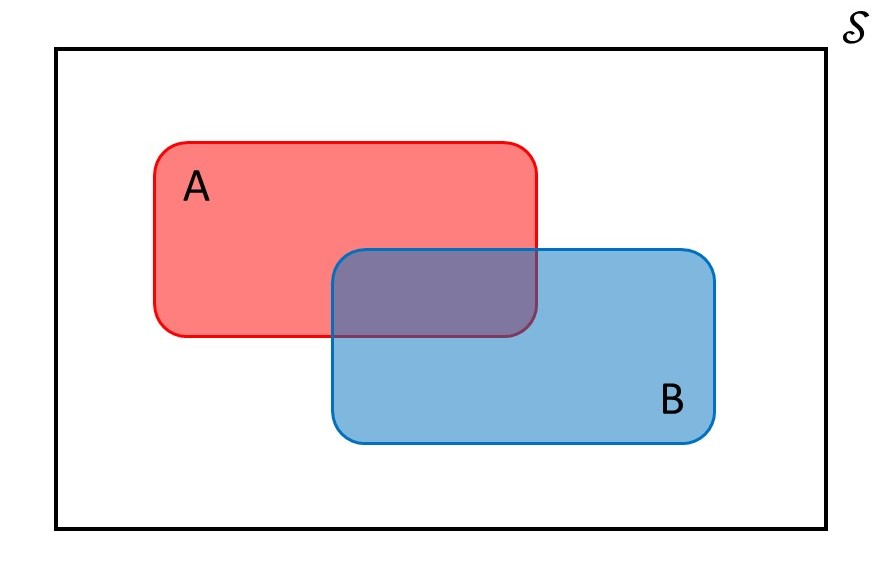
\includegraphics{images/RandomnessVennDiagram.jpg}

}

\caption{\label{fig-fundamentals-venn-diagram}Venn-Diagram illustrating
two events, \(A\) and \(B\), within a sample space \(\mathcal{S}\).}

\end{figure}

\begin{tcolorbox}[enhanced jigsaw, leftrule=.75mm, coltitle=black, left=2mm, title=\textcolor{quarto-callout-tip-color}{\faLightbulb}\hspace{0.5em}{Big Idea}, breakable, toptitle=1mm, bottomtitle=1mm, colback=white, colbacktitle=quarto-callout-tip-color!10!white, titlerule=0mm, opacitybacktitle=0.6, colframe=quarto-callout-tip-color-frame, bottomrule=.15mm, arc=.35mm, opacityback=0, rightrule=.15mm, toprule=.15mm]

Probability represents an area.

\end{tcolorbox}

\hypertarget{essential-results}{%
\section{Essential Results}\label{essential-results}}

While the Axioms of Probability (Definition~\ref{def-axioms}) set the
foundation, we can combine these axioms to form a set of rules which can
be employed to describe a myriad of scenarios. The first rule we review
states that the probability of an event not occurring is equivalent to
subtracting the probability it does occur from 1.

\begin{theorem}[Complement
Rule]\protect\hypertarget{thm-complement-rule}{}\label{thm-complement-rule}

For any event \(A\), the probability of its complement \(A^c\) is given
by

\[Pr\left(A^c\right) = 1 - Pr(A).\]

\end{theorem}

Our interest is not in rigorously developing probability theory; so, we
will offer many results without proof. However, to illustrate the
connection to the axioms, note that the Complement Rule is a result of
the second and third axioms. The second axiom tells us the probability
of the sample space is 1, and the third axiom allows us to consider the
probability of the union of two mutually exclusive events (which an
event and its complement are by definition).

The second rule we consider generalizes the third axiom. The third axiom
considers the union of mutually exclusive events, and the Addition Rule
defines the probability for the union of arbitrary events.

\begin{theorem}[Addition
Rule]\protect\hypertarget{thm-addition-rule}{}\label{thm-addition-rule}

Let \(A\) and \(B\) be arbitrary events, the probability of the union
\(A \cup B\) is given by

\[Pr(A \cup B) = Pr(A) + Pr(B) - Pr(A \cap B)\]

where \(A \cap B\) represents the intersection of the two events.

\end{theorem}

A very helpful technique in mathematical proofs is to ``do nothing.''
This technique will be a recurring theme later in the text and manifests
itself in adding nothing (adding and subtracting the same quantity to an
expression) or multiplying by one (multiplying and dividing an
expression by the same quantity).

\begin{theorem}[Total Probability
Rule]\protect\hypertarget{thm-total-probability-rule}{}\label{thm-total-probability-rule}

Let \(A\) and \(B\) be arbitrary events. Then,

\[Pr(A) = Pr(A \cap B) + Pr\left(A \cap B^c\right).\]

\end{theorem}

Though different than the proof you would likely encounter in a
Probability text, we provide the proof below because it illustrates the
``do nothing'' technique that will be helpful later on.

\begin{proof}

Let \(A\) and \(B\) be arbitrary events. We note that
\(A \cap \mathcal{S}\) is the set \(A\). And, since the intersection of
any set with itself is itself (like multiplying by 1, or ``doing
nothing'' to the set), we have

\[Pr(A) = Pr(A \cap \mathcal{S}).\]

Now, we recognize that an event and its complement together form the
sample space; therefore, we can write

\[Pr(A \cap \mathcal{S}) = Pr\left(A \cap \left(B \cup B^c\right)\right).\]

Using a distributive law from set theory, we write this probability as

\[Pr\left(A \cap \left(B \cup B^c\right)\right) = Pr\left((A \cap B) \cup \left(A \cap B^c\right)\right).\]

We now recognize that the events \((A \cap B)\) and
\(\left(A \cap B^c\right)\) are mutually exclusive. Therefore, applying
the third axiom of probability, we have that

\[Pr\left((A \cap B) \cup \left(A \cap B^c\right)\right) = Pr(A \cap B) + Pr\left(A \cap B^c\right)\]

giving the desired result.

\end{proof}

We have described probability as an ``area,'' and the above results
describe various ways of computing that area. However, occasionally we
are given additional information that changes the likelihood of an
event. Suppose we are interested in the probability an individual makes
a shot from the half-court line on a basketball court. Now, suppose we
are told the individual plays for the NBA; our probability should
reflect this additional knowledge. This is the idea of ``conditional
probability.''

\begin{theorem}[Conditional
Probability]\protect\hypertarget{thm-conditional-probability}{}\label{thm-conditional-probability}

Let \(A\) and \(B\) be arbitrary events. Then, the probability of \(A\)
given that \(B\) will occur is given by

\[Pr(A \mid B) = \frac{Pr(A \cap B)}{Pr(B)},\]

where we read \(A \mid B\) as ``A given B.''

\end{theorem}

Conditional probability assumes \(Pr(B) > 0\); it would not make sense
to condition on an event that will not occur. While there are many other
rules that are interesting and useful in application, the above rules
suffice for our purposes.

\hypertarget{interpretation-of-probability}{%
\section{Interpretation of
Probability}\label{interpretation-of-probability}}

Again, most probability courses are focused on the mathematics of
probability; as a result, rarely is the \emph{interpretation} of
probability discussed. In fact, most individuals rarely think about what
they mean by ``the probability an event occurs.'' From a mathematical
perspective, as long as we obey the Axioms of Probability
(Definition~\ref{def-axioms}), we have a probability; its meaning is
irrelevant. But, for practitioners, the interpretation is critical. As
it turns out, there are multiple interpretations of
probability\footnote{See the
  ``\href{https://plato.stanford.edu/archives/win2012/entries/probability-interpret/\#MaiInt}{Interpretations
  of Probability}'' entry in the Stanford Encyclopedia of Philosophy.}.
Two interpretations are of particular interest to us. To illustrate,
consider the following scenario.

\begin{example}[Sugar
Packets]\protect\hypertarget{exm-sugar}{}\label{exm-sugar}

Restaurants can be sources of anxiety for small children. After placing
their order, they must wait (for what seems like an eternity) for that
food to arrive. This is different from their experience at home where
they typically are not brought to the table until it is time to eat.
Parents spend a lot of effort entertaining their children while waiting
for their food to arrive. For parents who do not want to limit screen
time, the following simple game is surprisingly effective:

\begin{quote}
Take one of the sugar packets that is generally available at the table.
Denote the side with the brand name as the ``top side'' and denote the
side with the ingredient list as the ``bottom side.'' The parent then
takes the sugar packet and, hidden from view, tumbles the packet
randomly in their hands. The packet is then placed on the table under
the cover of the parent's hand. The child then declares which side of
the packet is facing up by saying ``top side'' or ``bottom side.''
\end{quote}

This is similar to flipping a coin, but who carries change with them
these days? Consider one round of the above game; suppose the (covered)
packet has been placed on the table and the child says ``top side.'' The
question we ask is then ``what is the probability the child is
correct?''

\end{example}

This simple example illustrates the two commonly applied interpretations
of probability. Most people will say the probability the child is
correct is 0.5. The reasoning is that there are two possibilities (the
top of the sugar packet is face up; or, the bottom of the sugar packet
is face up), and these two possibilities are equally likely (since it
was randomly shuffled before being placed on the table). Therefore, the
probability the child is correct is 0.5. \textbf{From a classical view
of statistics, this interpretation is incorrect.} The complication here
is what we believe probability is capturing.

From a classical (or ``Frequentist'') perspective, probability is
capturing the likelihood of an event across repeated trials. From a
Bayesian perspective, however, probability is used to quantify our
uncertainty. That is, from the Bayesian perspective the phrase ``the
probability the child is correct is 0.5'' is not actually quantifying
the likelihood the child is correct --- it is quantifying our
uncertainty the child is correct. We are only ``50\% sure'' the child is
correct. This relies on the ``subjective interpretation'' of
probability.

\begin{definition}[Subjective Interpretation of
Probability]\protect\hypertarget{def-subjective-interpretation}{}\label{def-subjective-interpretation}

In this perspective, the probability of \(A\) describes the individual's
uncertainty about event \(A\).

\end{definition}

Because the subjective interpretation is quantifying an individual's
uncertainty, and since each individual may have different
beliefs/information/expertise about the random process, each individual
observing the same process may have a different probability. For
example, consider asking the question ``what is the probability that
Netflix saves the latest television series dropped by ABC?'' A casual
viewer may have little information regarding this process and will rely
solely on what they perceive the popularity of the show was among its
fan base and news reports they have read online; they may quantify their
uncertainty by saying the probability is 0.65. In contrast, an executive
at Netflix who is deeply familiar with both the show, its fan base, its
ratings in various markets, the interest of leadership to invest in a
new series, and the amount they stand to earn by acquiring the property
has a different set of knowledge; they may quantify their uncertainty by
saying the probability is 0.05. The same process is viewed differently
by different observers, leading to different answers.

Statisticians who adhere to the subjective interpretation of probability
are known as Bayesians. Classically, statistical theory was developed
under the frequentist interpretation, and statisticians who adhere to
this perspective are known as Frequentists.

\begin{definition}[Frequentist Interpretation of
Probability]\protect\hypertarget{def-frequentist-interpretation}{}\label{def-frequentist-interpretation}

In this perspective, the probability of \(A\) describes the long-run
behavior of the event. Specifically, consider repeating the random
process \(m\) times, and let \(f(A)\) represent the number of times the
event \(A\) occurs out of those \(m\) replications. Then,

\[Pr(A) = \lim_{m \rightarrow \infty} \frac{f(A)}{m}.\]

\end{definition}

The frequentist interpretation requires repeating a process infinitely
often. When characterizing the probability of an event, the frequentist
perspective leans on the future-oriented nature of probability. When we
are characterizing the probability an event \emph{will} occur
(future-oriented), we are really thinking about repeating that process
infinitely often and determining what fraction of the time the event
occurs; we then apply that to the specific process we are about to
observe. Of course, this does not always make sense in practice. For
example, asking ``what is the probability that Candidate A will win the
upcoming election'' is a one time event. The election cannot be held
infinitely often; it will only be held once. In these cases, the
frequentist interpretation still \emph{imagines} infinitely many of
these elections. For those who are fans of science fiction, you can
think of the frequentist perspective as finding the limit over the
infinitely many instances in the multiverse (the proportion of times
Candidate A wins the election across all instances of the election in
the multiverse). The frequentist perspective is ``objective'' in the
sense that it does not incorporate the observer's personal
beliefs/information/expertise regarding the process.

Returning to Example~\ref{exm-sugar}, since the result has already
occurred, probability does not make sense. Further, since the
frequentist perspective does not quantify our uncertainty about the
result (as the subjective perspective does), we are left saying that the
probability that the child is correct is either 1 (they are correct) or
0 (they are not correct). Admittedly, this is unsatisfying, but we must
remember that the frequentist interpretation is not interested in
quantifying our uncertainty; it is only interested in the proportion of
times the result will occur, and since the result is in the past, it
either has occurred (proportion of 1) or it has not (proportion of 0).

This may seem like arguing over semantics, and admittedly, the
importance of this discussion is not yet clear. But, we will see that
how probability is interpreted impacts how we interpret the results of
our statistical analyses.

\begin{tcolorbox}[enhanced jigsaw, leftrule=.75mm, coltitle=black, left=2mm, title=\textcolor{quarto-callout-tip-color}{\faLightbulb}\hspace{0.5em}{Big Idea}, breakable, toptitle=1mm, bottomtitle=1mm, colback=white, colbacktitle=quarto-callout-tip-color!10!white, titlerule=0mm, opacitybacktitle=0.6, colframe=quarto-callout-tip-color-frame, bottomrule=.15mm, arc=.35mm, opacityback=0, rightrule=.15mm, toprule=.15mm]

The frequentist interpretation of probability quantifies the likelihood
of an event in repeated observation, and the subjective interpretation
quantifies our uncertainty of an event.

\end{tcolorbox}

As this text focuses on the Bayesian perspective, we adopt the
subjective interpretation of probability throughout. Note that this
means that two analysts can approach the same problem in the same way
and end up with a different conclusion if they have different beliefs!

\hypertarget{sec-randomvariables}{%
\chapter{Random Variables and Distributions}\label{sec-randomvariables}}

\providecommand{\norm}[1]{\lVert#1\rVert}
\providecommand{\abs}[1]{\lvert#1\rvert}
\providecommand{\iid}{\stackrel{\text{IID}}{\sim}}
\providecommand{\ind}{\stackrel{\text{Ind}}{\sim}}

\providecommand{\bm}[1]{\mathbf{#1}}
\providecommand{\bs}[1]{\boldsymbol{#1}}
\providecommand{\bbeta}{\bs{\beta}}

\providecommand{\Ell}{\mathcal{L}}
\providecommand{\indep}{\perp\negthickspace\negmedspace\perp}

In Chapter~\ref{sec-fundamentals}, we discussed the probability of an
``event.'' For statisticians, the events of interests center on
measurements, or functions of those measurements, that we plan to take.
In this chapter, we begin to connect probability to data analysis. Our
goal is to reexamine concepts introduced in a probability course,
relating them to their data-centric analogues, which will be discussed
further in the next unit.

\hypertarget{random-variables}{%
\section{Random Variables}\label{random-variables}}

Consider collecting data; before the data is collected, we cannot
predict with certainty what we will observe. Therefore, we can think of
each observation as the result of a random process. These observations
are recorded as variables in our dataset. In probability, a
\textbf{random variable} is used to represent a measurement that results
from a random process.

\begin{definition}[Random
Variable]\protect\hypertarget{def-random-variable}{}\label{def-random-variable}

Let \(\mathcal{S}\) be the sample space corresponding to a random
process; a random variable \(X\) is a function mapping elements of the
sample space to the real line.

Random variables represent a measurement that will be collected during
the course of a study. Random variables are typically represented by a
capital letter.

\end{definition}

While for our purposes, it suffices to think of a random variable as a
measurement, mathematically, it is a \emph{function}. The image (or
range) of this function is used to broadly classify random variables as
\textbf{continuous} or \textbf{discrete}; we refer to this image as the
\textbf{support} of the random variable.

\begin{definition}[Support]\protect\hypertarget{def-support}{}\label{def-support}

The support of a random variable is the set of all possible values the
random variable can take.

\end{definition}

\begin{definition}[Continuous and Discrete Random
Variable]\protect\hypertarget{def-rvtypes}{}\label{def-rvtypes}

The random variable \(X\) is said to be a discrete random variable if
its corresponding support is countable. The random variable \(X\) is
said to be a continuous random variable if the corresponding support is
uncountable (such as an interval or a union of intervals on the real
line).

\end{definition}

Discrete random variables are analogous to categorical (or qualitative)
variables in data analysis; that is, discrete random variables are used
to model the result of a random process which categorizes each unit of
observation into a group. Continuous random variables are analogous to
numeric (or quantitative) variables in data analysis; continuous random
variables are used to model the result of a random process which
produces a number for which arithmetic makes sense.

\begin{tcolorbox}[enhanced jigsaw, leftrule=.75mm, coltitle=black, left=2mm, title=\textcolor{quarto-callout-warning-color}{\faExclamationTriangle}\hspace{0.5em}{Warning}, breakable, toptitle=1mm, bottomtitle=1mm, colback=white, colbacktitle=quarto-callout-warning-color!10!white, titlerule=0mm, opacitybacktitle=0.6, colframe=quarto-callout-warning-color-frame, bottomrule=.15mm, arc=.35mm, opacityback=0, rightrule=.15mm, toprule=.15mm]

Whether we use a continuous or discrete random variable to represent a
measurement is not always obvious. Suppose we consider recording the age
of a student selected from a class at a university that typically
enrolls ``traditional'' students (those coming directly from high
school). Let the random variable \(X\) denote the age of the student.

If we record the student's age in years since birth, \(X\) can take on
only a finite number of values (most likely
\(\{18, 19, 20, 21, 22, 23\}\)), making it a discrete random variable.
However, if we record the student's age as the number of seconds since
birth, we might well consider the support of \(X\) to be a rather large
interval, leading to a continuous random variable.

\end{tcolorbox}

The goal of statistics is to use a sample to say something about the
underlying population. Consider taking a sample of size \(n\) and
measuring a single variable on each unit of observation. Then, we might
represent the measurements we will obtain (note the use of the future
tense) as \(X_1, X_2, \dots, X_n\). While the majority of probability
courses focus on a single, or maybe two, random variables, note that
collecting data on a sample requires that we deal with at least \(n\)
random variables (one measurement for each of the observations in our
sample).

\hypertarget{characterizing-a-distribution}{%
\section{Characterizing a
Distribution}\label{characterizing-a-distribution}}

Again, the goal of statistics is to use a sample to say something about
the underlying population. Consider the following research objective:

\begin{quote}
Estimate the cost (in US dollars) of a diamond for sale in the United
States.
\end{quote}

For this research objective, our population of interest is all diamonds
for sale in the United States. We would not expect every diamond for
sale to have the same price; variability is inherent in any process. As
a result, the sale price of diamonds has a distribution across this
population. This is our primary use of probability theory in a
statistical analysis --- to model distributions.

Consider taking a sample of size 1 from the population; let \(Y\)
represent the cost of the diamond that is selected. Since we have not
yet observed the cost of this diamond, \(Y\) is a random variable. And,
since this diamond is sampled from the population of interest, the
support of \(Y\) is determined by the cost of diamonds in the United
States. Further, the likelihood that \(Y\) falls within any interval is
determined by the distribution of the cost across the population. That
is, the distribution of \(Y\) is the distribution of the population.

\begin{tcolorbox}[enhanced jigsaw, leftrule=.75mm, coltitle=black, left=2mm, title=\textcolor{quarto-callout-tip-color}{\faLightbulb}\hspace{0.5em}{Big Idea}, breakable, toptitle=1mm, bottomtitle=1mm, colback=white, colbacktitle=quarto-callout-tip-color!10!white, titlerule=0mm, opacitybacktitle=0.6, colframe=quarto-callout-tip-color-frame, bottomrule=.15mm, arc=.35mm, opacityback=0, rightrule=.15mm, toprule=.15mm]

If a random variable \(X\) represents a measurement for a single
observation from a population, the distribution of the random variable
corresponds to the distribution of the variable across the population.

\end{tcolorbox}

A key realization in statistical analysis is that we will never fully
observe the distribution of the population; however, we can posit a
model for this distribution. In probability, the most common way to
characterize the distribution of a random variable is through its
density function.

\begin{definition}[Density
Function]\protect\hypertarget{def-density-function}{}\label{def-density-function}

A density function \(f\) relates the values in the support of a random
variable with the probability of observing those values.

Let \(X\) be a continuous random variable, then its density function
\(f\) is the function such that

\[Pr(a \leq X \leq b) = \int_a^b f(x) dx\]

for any real numbers \(a\) and \(b\) in the support.

Let \(X\) be a discrete random variable, then its density function \(f\)
is the function such that

\[Pr(X = u) = f(u)\]

for any real number \(u\) in the support.

\end{definition}

\begin{tcolorbox}[enhanced jigsaw, leftrule=.75mm, coltitle=black, left=2mm, title=\textcolor{quarto-callout-note-color}{\faInfo}\hspace{0.5em}{Properties of a Density Function}, breakable, toptitle=1mm, bottomtitle=1mm, colback=white, colbacktitle=quarto-callout-note-color!10!white, titlerule=0mm, opacitybacktitle=0.6, colframe=quarto-callout-note-color-frame, bottomrule=.15mm, arc=.35mm, opacityback=0, rightrule=.15mm, toprule=.15mm]

Let \(X\) be a random variable with density function \(f\) defined over
support \(\mathcal{S}\). Then,

\begin{enumerate}
\def\labelenumi{\arabic{enumi}.}
\tightlist
\item
  \(f(x) \geq 0\) for all \(x \in \mathcal{S}\). That is, the density is
  non-negative for all values in the support.
\item
  If \(X\) is a continuous random variable, then
  \(\int_{\mathcal{S}} f(x) dx = 1\); similarly, if \(X\) is a discrete
  random variable, then \(\sum_{\mathcal{S}} f(x) = 1\). That is, \(X\)
  must take a value in its support; so, \(Pr(X \in \mathcal{S}) = 1\),
  similar to the second Axiom of Probability
  (Definition~\ref{def-axioms}).
\item
  \(f(x) = 0\) for all values of \(x \notin \mathcal{S}\). The density
  takes the value of 0 for all values outside the support.
\end{enumerate}

\end{tcolorbox}

\begin{tcolorbox}[enhanced jigsaw, leftrule=.75mm, coltitle=black, left=2mm, title=\textcolor{quarto-callout-note-color}{\faInfo}\hspace{0.5em}{Note}, breakable, toptitle=1mm, bottomtitle=1mm, colback=white, colbacktitle=quarto-callout-note-color!10!white, titlerule=0mm, opacitybacktitle=0.6, colframe=quarto-callout-note-color-frame, bottomrule=.15mm, arc=.35mm, opacityback=0, rightrule=.15mm, toprule=.15mm]

In a probability course, there is often a distinction made between
probability ``density'' functions (used for continuous random variables)
and probability ``mass'' functions (used for discrete random variables).
We do not make this distinction and instead rely on the context to
determine whether we are dealing with a continuous or discrete random
variable. Throughout, we will note when the operations differ between
these two types of variables. Measure theory provides a unifying
framework to these issues.

\end{tcolorbox}

When working with a continuous random variable, the density function is
a smooth function over some region, and the actual value of the function
is not interpretable; instead, we get at a probability by considering
the area under the curve. Again, drawing connections to data analysis,
we can think of a density function as a mathematical formula
representing a smooth histogram. The area under the curve for any region
gives the proportion of the population which has a value in that region.
That is, we get the probability that a random variable will be in an
interval by integrating the density function over that interval.

Figure Figure~\ref{fig-randomvariables-density} illustrates this idea;
we have data from a sample of diamonds from the population of interest.
The sample is summarized with a histogram; we have overlayed a posited
density (with the corresponding mathematical function that describes
this density) for the population. The sample (summarized with the
histogram) is approximating the population (modeled using the density
function).

\begin{figure}

{\centering 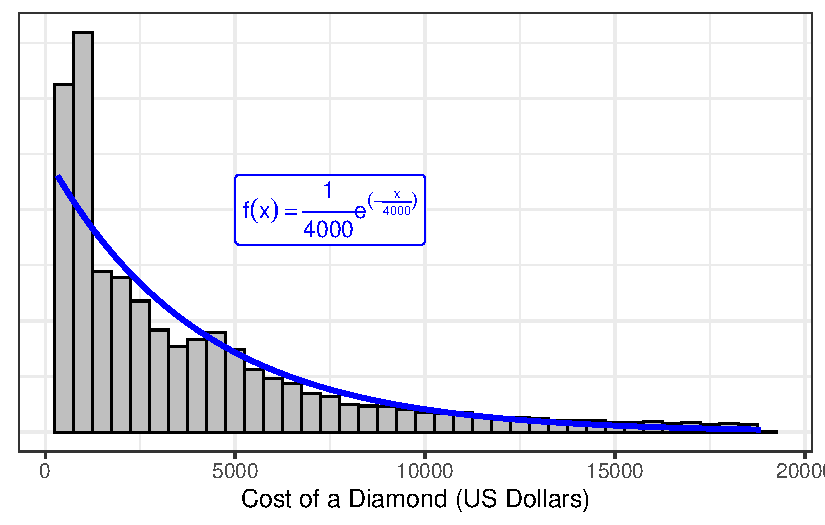
\includegraphics[width=0.8\textwidth,height=\textheight]{./images/fig-randomvariables-density-1.pdf}

}

\caption{\label{fig-randomvariables-density}Illustration of a density
function representing the posited distribution of the population
alongside a histogram summarizing the cost of diamonds using a sample of
53940 diamonds.}

\end{figure}

You may recognize the particular form of the density function in
Figure~\ref{fig-randomvariables-density}. The general form is

\[f(x) = \frac{1}{\sigma} e^{-x / \sigma} \qquad \text{for } x > 0\]

where \(\sigma\) is the \emph{scale} parameter that defines the
distribution (set at 4000 in Figure~\ref{fig-randomvariables-density}).
This is known as the Exponential distribution with scale parameter
\(\sigma\). This illuminates another connection between probability and
statistics.

Note that our research objective describe above is an ill-posed question
as stated. The answer is ``it depends'' since each individual diamond in
the population has a different value. Well-posed questions in statistics
are centered on an appropriately chosen \textbf{parameter}
(Definition~\ref{def-parameter}).

In probability, the parameters are values that are tuned or set within a
problem; we then work forward to compute the probability of an event of
interest. In practice, however, when we posit a functional form for a
density function to describe the distribution of the population, the
parameters are unknown. We plan to use the data to estimate or
characterize the parameter; but, the parameter itself will remain
unknown. In both cases, however, the parameter is a \emph{fixed
quantity}, even if we are ignorant of that value.

\begin{tcolorbox}[enhanced jigsaw, leftrule=.75mm, coltitle=black, left=2mm, title=\textcolor{quarto-callout-tip-color}{\faLightbulb}\hspace{0.5em}{Big Idea}, breakable, toptitle=1mm, bottomtitle=1mm, colback=white, colbacktitle=quarto-callout-tip-color!10!white, titlerule=0mm, opacitybacktitle=0.6, colframe=quarto-callout-tip-color-frame, bottomrule=.15mm, arc=.35mm, opacityback=0, rightrule=.15mm, toprule=.15mm]

When a probability model is specified for a population, it is generally
specified up to some unknown parameter(s). Making inference on the
unknown parameter(s) therefore characterizes the entire distribution.

\end{tcolorbox}

\hypertarget{common-parameters}{%
\subsection{Common Parameters}\label{common-parameters}}

Most scientific questions are focused on the location or spread of a
distribution. For example, we are interested in estimating the average
cost of a diamond sold in the United States. Introductory statistics
introduces summaries of location and spread within the sample (e.g.,
sample mean for location and sample variance for spread). Analogous
summaries exist for density functions. As stated above, parameters are
unknown constants that govern the form of the density function. Because
they govern the form of the density, the parameters are also related to
those summarizing the location or spread of the distribution.

\begin{definition}[Expected Value
(Mean)]\protect\hypertarget{def-mean}{}\label{def-mean}

Let \(X\) be a random variable with density function \(f\) defined over
the support \(\mathcal{S}\). The expected value of a random variable,
also called the mean and denoted \(E(X)\), is given by

\[E(X) = \int_{\mathcal{S}} x f(x) dx\]

for continuous random variables and

\[E(X) = \sum_{\mathcal{S}} x f(x)\]

for discrete random variables.

\end{definition}

Notice the similarity between the form of the sample mean and the
population mean. A sample mean takes the sum of each value in the
sample, weighting each value by \(1/n\) (where \(n\) is the sample
size). Without information about the underlying population, the sample
must treat each value observed as equally likely; values become more
likely if they appear multiple times. In the population, however, when
the form of \(f\) is known, the density provides information about the
likelihood of each value giving us a better weight than \(1/n\). That
is, the population mean is a sum of the values in the support, weighting
each value by the corresponding value of the density function.

\begin{definition}[Variance]\protect\hypertarget{def-variance}{}\label{def-variance}

Let \(X\) be a random variable with density function \(f\) defined over
the support \(\mathcal{S}\). The variance of a random variable, denoted
\(Var(X)\), is given by

\[Var(X) = E\left[X - E(X)\right]^2 = E\left(X^2\right) - E^2(X).\]

If we let \(\mu = E(X)\), then this is equivalent to

\[\int_{\mathcal{S}} (x - \mu)^2 f(x) dx\]

for continuous random variables and

\[\sum_{\mathcal{S}} (x - \mu)^2 f(x)\]

for discrete random variables.

\end{definition}

\begin{tcolorbox}[enhanced jigsaw, leftrule=.75mm, coltitle=black, left=2mm, title=\textcolor{quarto-callout-warning-color}{\faExclamationTriangle}\hspace{0.5em}{Warning}, breakable, toptitle=1mm, bottomtitle=1mm, colback=white, colbacktitle=quarto-callout-warning-color!10!white, titlerule=0mm, opacitybacktitle=0.6, colframe=quarto-callout-warning-color-frame, bottomrule=.15mm, arc=.35mm, opacityback=0, rightrule=.15mm, toprule=.15mm]

Pay careful attention to the notation. \(E^2(X)\) represents the square
of the expected value; that is,

\[E^2(X) = \left[E(X)\right]^2.\]

However, \(E(X)^2\) represents the expected value of the square of
\(X\); that is,

\[E(X)^2 = E\left(X^2\right).\]

\end{tcolorbox}

The variance provides a measure of spread; in particular, it is
capturing distance from the mean. Notice that the form of the variance
involves taking the expectation of a squared term; in general, we will
need to consider expectations of functions.

\begin{definition}[Expectation of a
Function]\protect\hypertarget{def-expectation}{}\label{def-expectation}

Let \(X\) be a random variable with density function \(f\) over the
support \(\mathcal{S}\), and let \(g\) be a real-valued function. Then,

\[E\left[g(X)\right] = \int_{\mathcal{S}} g(x) f(x) dx\]

for continuous random variables and

\[E\left[g(X)\right] = \sum_{\mathcal{S}} g(x) f(x)\]

for discrete random variables.

\end{definition}

\begin{tcolorbox}[enhanced jigsaw, leftrule=.75mm, coltitle=black, left=2mm, title=\textcolor{quarto-callout-note-color}{\faInfo}\hspace{0.5em}{Note}, breakable, toptitle=1mm, bottomtitle=1mm, colback=white, colbacktitle=quarto-callout-note-color!10!white, titlerule=0mm, opacitybacktitle=0.6, colframe=quarto-callout-note-color-frame, bottomrule=.15mm, arc=.35mm, opacityback=0, rightrule=.15mm, toprule=.15mm]

Definition~\ref{def-expectation} is sometimes referred to as the ``Law
of the Unconscious Statistician'' in probability texts. We find the name
somewhat insulting, as it suggests statisticians do not appreciate the
mathematical underpinnings of their field. In reality, the expected
value of a function is such a common operation in statistical theory
that statisticians often present Definition~\ref{def-expectation} as the
definition of an expectation (as we have done) instead of deriving it as
a result of Definition~\ref{def-mean} after applying a variable
transformation (see Example~\ref{exm-transformations} below). It is
possible this is where the slight in the naming convention originated.

\end{tcolorbox}

A result of Definition~\ref{def-expectation} is the following, very
useful theorem, which states that expectations are linear operators.

\begin{theorem}[Expectation of a Linear
Combination]\protect\hypertarget{thm-expectation}{}\label{thm-expectation}

Let \(X\) be a random variable, and let \(a_1, a_2, \dotsc, a_m\) be
real-valued constants and \(g_1, g_2, \dotsc, g_m\) be real-valued
functions; then,

\[E\left[\sum_{i=1}^{m} a_i g_i(X)\right] = \sum_{i=1}^{m} a_i E\left[g_i(X)\right].\]

\end{theorem}

The mean and variance play an important role in characterizing a
distribution, especially within statistical theory (as we will see in
future chapters). However, there is another set of parameters which are
important.

\begin{definition}[Percentile for a Random
Variable]\protect\hypertarget{def-population-percentile}{}\label{def-population-percentile}

Let \(X\) be a random variable with density function \(f\). The \(100k\)
percentile is the value \(q\) such that

\[Pr(X \leq q) = k.\]

\end{definition}

\begin{example}[Parameters of Exponential
Distribution]\protect\hypertarget{exm-parameters}{}\label{exm-parameters}

Let \(X\) be an Exponential distribution with scale parameter
\(\sigma\); that is, the density function \(f\) is given by

\[f(x) = \frac{1}{\sigma} e^{-x/\sigma} \qquad x > 0\]

where \(\sigma > 0.\) Compute the mean, variance, and median of this
distribution, as a function of the unknown scale parameter.

\end{example}

The solution to this problem is particularly important as it illustrates
a very useful technique when working with known distributions in
statistical theory.

\begin{solution}

We note that the function

\[g(y) = \frac{1}{\beta^{\alpha} \Gamma(\alpha)} y^{\alpha - 1} e^{-y/\beta}\]

is a valid density function over the positive real line provided that
\(\alpha,\beta > 0\); in particular, this is known as a Gamma
distribution. Since \(g\) is a valid density function, then we know that

\[\int_{0}^{\infty} g(y) dy = 1\]

for all values of \(\alpha,\beta > 0\).

Now, let \(X\) be an Exponential random random variable with scale
parameter \(\sigma\). Then, the expected value of \(X\) is given by

\[
\begin{aligned}
  E(X)
    &= \int_{0}^{\infty} x \frac{1}{\sigma} e^{-x/\sigma} dx \\
    &= \int_{0}^{\infty} \frac{1}{\sigma} x^{2-1} e^{-x/\sigma} dx
\end{aligned}
\]

where we have simply rewritten the exponent in the second line. Notice
that expression within the integral shares a striking similarity to the
form of the density function of a Gamma distribution; however, they are
not exactly the same. To coerce the expression into that of the Gamma
density function, we ``do nothing'' --- multiplying and dividing the
expression by the quantity \(\sigma\Gamma(2)\). This gives

\[
\begin{aligned}
  E(X)
    &= \int_{0}^{\infty} x \frac{1}{\sigma} e^{-x/\sigma} dx \\
    &= \int_{0}^{\infty} \frac{1}{\sigma} x^{2-1} e^{-x/\sigma} dx \\
    &= \int_{0}^{\infty} \sigma \Gamma(2) \frac{1}{\sigma^2 \Gamma(2)} x^{2-1} e^{-x/\sigma} dx \\
    &= \sigma \Gamma(2) \int_{0}^{\infty} \frac{1}{\sigma^2 \Gamma(2)} x^{2-1} e^{-x/\sigma} dx \\
    &= \sigma \Gamma(2) \\
    &= \sigma.
\end{aligned}
\]

In line 3, we have multiplied and divided by \(\sigma \Gamma(2)\), which
does not change the problem. In line 4, we have pulled out the terms
\(\sigma \Gamma(2)\) since it is a constant with respect to the
integral; what is left inside the integral is the form of the density
function for a Gamma distribution where \(\alpha = 2\) and
\(\beta = \sigma\). In line 5, we make use of the fact that the integral
of any density function over the entire support for which it is defined
must be 1. Finally, in line 6, we recognize that \(\Gamma(k) = (k-1)!\)
if \(k\) is a natural number.

Applying the same process, we also have that

\[
\begin{aligned}
  E\left(X^2\right)
    &= \int_{0}^{\infty} x^2 \frac{1}{\sigma} e^{-x/\sigma} dx \\
    &= \sigma^2 \Gamma(3)\int_{0}^{\infty} \frac{1}{\sigma^3 \Gamma(3)} x^{3-1} e^{-x/\sigma} dx \\
    &= 2\sigma^2.
\end{aligned}
\]

Therefore,

\[Var(X) = E\left(X^2\right) - E^2(X) = 2\sigma^2 - \sigma^2 = \sigma^2.\]

Finally, the median is the value \(q\) such that \(Pr(X \leq q) = 0.5\);
but, we recognize that

\[
\begin{aligned}
  Pr(X \leq q) 
    &= \int_{0}^{q} \frac{1}{\sigma} e^{-x/\sigma} dx \\
    &= \left. -e^{-x/\sigma} \right|_{0}^{q} \\
    &= -e^{-q/\sigma} + 1.
\end{aligned}
\]

Setting this expression equal to 0.5 and solving for \(q\) yields
\(q = -\sigma \log(0.5)\), where \(\log(\cdot)\) represents the
\emph{natural} logarithm.

\end{solution}

\begin{tcolorbox}[enhanced jigsaw, leftrule=.75mm, coltitle=black, left=2mm, title=\textcolor{quarto-callout-tip-color}{\faLightbulb}\hspace{0.5em}{Big Idea}, breakable, toptitle=1mm, bottomtitle=1mm, colback=white, colbacktitle=quarto-callout-tip-color!10!white, titlerule=0mm, opacitybacktitle=0.6, colframe=quarto-callout-tip-color-frame, bottomrule=.15mm, arc=.35mm, opacityback=0, rightrule=.15mm, toprule=.15mm]

Suppose the density \(f\) is a function of the parameters
\(\boldsymbol{\theta}\); then, the mean, variance, and median (as well
as any other parameters of interest in a research objective) will be
functions of \(\boldsymbol{\theta}\).

\end{tcolorbox}

Example~\ref{exm-parameters} highlighted a useful technique for
simplifying integrals in statistical applications, which makes use of
the ``do nothing'' strategy discussed in the previous chapter.

\hypertarget{kernels}{%
\subsection{Kernels}\label{kernels}}

One of the characteristics common to any density function that we noted
above was that if we sum the density across the entire support, we get a
value of 1. That is, if \(X\) is a discrete random variable, then

\[\sum_{x \in \mathcal{S}_X} f(x) = 1,\]

and if \(X\) is a continuous random variable, then

\[\int_{\mathcal{S}_X} f(x) dx = 1.\]

Any density function can be written as

\[f(x) = a k(x)\]

where \(a > 0\) is a constant and \(k(x)\) is a function of \(x\).
Specifically, if \(X\) is a continuous random variable, then

\[a = \frac{1}{\int k(x) dx}\]

since \(\int f(x) dx = 1\). We call \(k(x)\) the \textbf{kernel} of the
distribution. Kernels are helpful for quickly identifying
distributions\footnote{A good
  \href{https://qiangbo-workspace.oss-cn-shanghai.aliyuncs.com/2018-11-11-common-probability-distributions/distab.pdf}{table
  of common distributions} is given in Casella and Berger, a popular
  text for statistical theory at the graduate level.}.

\begin{definition}[Kernel of a
Distribution]\protect\hypertarget{def-kernel}{}\label{def-kernel}

Let \(k(x)\) be a non-negative function of \(x\) over some region
\(\mathcal{S}_X\). Then, a valid density function \(f\) over the support
\(\mathcal{S}_X\) can be constructed by taking

\[f(x) = a k(x)\]

where \(a > 0\) is a suitably chosen scaling constant to ensure the
density integrates (or sums) to 1 over the support. The function \(k\)
is known as the kernel of the distribution, and it can be used to
identify the distributional family for a random variable.

\end{definition}

\begin{example}[Kernel of an Exponential Random
Variable]\protect\hypertarget{exm-kernel}{}\label{exm-kernel}

In Example~\ref{exm-parameters}, we let \(X\) be an Exponential random
variable with scale parameter \(\sigma\). Identify the kernel of this
distribution.

\end{example}

\begin{solution}

Let \(a = \sigma^{-1}\) and

\[k(x) = e^{-x/\sigma};\]

then, we have that \(f(x) = a k(x)\). We note that \(k(x)\) has no
leading constants; therefore, the kernel for an Exponential distribution
is

\[e^{-x/\sigma}.\]

\end{solution}

As Example~\ref{exm-parameters} illustrated, being able to identify a
kernel can help us quickly evaluate an integral. In particular, notice
that we immediately have that

\[\int e^{-x/\sigma} dx = \sigma\]

for any value of \(\sigma > 0\) because we know that

\[
\begin{aligned}
  \int e^{-x / \sigma} dx 
    &= \sigma \int \frac{1}{\sigma} e^{-x / \sigma} dx \\
    &= \sigma.
\end{aligned}
\]

The first line multiplies and divides by the appropriate scaling term so
that the kernel becomes a valid density function. Once we have a valid
density, we know it integrates to 1, simplifying the expression.

In addition to motivating the use of kernels in integration
applications, the solution to Example~\ref{exm-parameters} also shows
that there is more than one way to characterize a distribution.

\hypertarget{distribution-function}{%
\subsection{Distribution Function}\label{distribution-function}}

Especially for visualization, the density function is the most common
way of characterizing a probability model. However, computing the
probability using the density is problematic due to the integration
required. Many software address this by working with the cumulative
distribution function (CDF).

\begin{definition}[Cumulative Distribution Function
(CDF)]\protect\hypertarget{def-cdf}{}\label{def-cdf}

Let \(X\) be a random variable; the cumulative distribution function
(CDF) is defined as

\[F(u) = Pr(X \leq u).\]

For a continuous random variable, we have that

\[F(u) = \int_{-\infty}^{u} f(x) dx\]

implying that the density function is the derivative of the CDF. For a
discrete random variable

\[F(u) = \sum_{x \leq u} f(x).\]

\end{definition}

Working with the CDF improves computation because it avoids the need to
integrate each time; instead, the integral is computed once (and stored
internally in the computer) and we use the result to compute
probabilities directly.

\begin{tcolorbox}[enhanced jigsaw, leftrule=.75mm, coltitle=black, left=2mm, title=\textcolor{quarto-callout-tip-color}{\faLightbulb}\hspace{0.5em}{Big Idea}, breakable, toptitle=1mm, bottomtitle=1mm, colback=white, colbacktitle=quarto-callout-tip-color!10!white, titlerule=0mm, opacitybacktitle=0.6, colframe=quarto-callout-tip-color-frame, bottomrule=.15mm, arc=.35mm, opacityback=0, rightrule=.15mm, toprule=.15mm]

Density functions are the mathematical models for distributions; they
link values of the variable with the likelihood of occurrence. However,
for computational reasons, we often work with the cumulative
distribution function which provides the probability of being less than
or equal to a value.

\end{tcolorbox}

\hypertarget{transformations-of-a-random-variable}{%
\section{Transformations of a Random
Variable}\label{transformations-of-a-random-variable}}

Occasionally, we are interested in a transformation of a particular
characteristic. That is, we have a model for the distribution of \(X\),
but we are interested in \(Y = g(X)\). In this section, we examine one
method for determining the density of \(Y\) from the density of \(X\).
While relationships between many common distributions have been well
studied\footnote{An excellent
  \href{http://www.math.wm.edu/~leemis/chart/UDR/UDR.html}{summary of
  the relationships between Distributions} was developed by faculty at
  the College of William and Mary.}, it is useful to know the process
for addressing transformations.

While there various approaches to this problem, we find this method the
most reliable. Further, it does not require the memorization of a
formula, but instead builds on fundamental ideals. This is known as the
\textbf{Method of Distribution Functions}.

\begin{definition}[Method of Distribution
Functions]\protect\hypertarget{def-method-of-distribution-functions}{}\label{def-method-of-distribution-functions}

Let \(X\) be a continuous random variable with density \(f\) and
cumulative distribution function \(F\). Consider \(Y = h(X)\). The
following process provides the density function \(g\) of \(Y\) by first
finding its cumulative distribution function \(G\).

\begin{enumerate}
\def\labelenumi{\arabic{enumi}.}
\tightlist
\item
  Find the set \(A\) for which \(h(X) \leq t\) if and only if
  \(X \in A\).
\item
  Recognize that
  \(G(y) = Pr(Y \leq y) = Pr\left(h(X) \leq y\right) = Pr(X \in A)\).
\item
  If interested in \(g(y)\), note that
  \(g(y) = \frac{\partial}{\partial y} G(y)\).
\end{enumerate}

\end{definition}

When \(h\) is a strictly monotone function (unique inverse exists), then
step 1-2 is much easier because we can apply \(h^{-1}\). In step 2 of
the above process, the final expression is often left in terms of \(F\),
the CDF of \(X\); then, when we find the density in step 3, we can apply
the chain rule (avoiding the need to actually have an expression for
\(F\)).

\begin{example}[Transformation of a Random
Variable]\protect\hypertarget{exm-transformations}{}\label{exm-transformations}

Previously, we posited the following model for the distribution of the
cost of a diamond sold in the US:

\[f(x) = \frac{1}{\sigma} e^{-x/\sigma} \qquad x > 0\]

for some \(\sigma > 0\). As cost is generally a heavily skewed variable,
we may be interested in taking the (natural) logarithm before proceeding
with an analysis. Find the density of \(Y = \log(X)\); then, write an
expression for \(E(Y)\).

\end{example}

\begin{solution}

We note that \(\log(x)\) is a strictly monotone function. Therefore, we
have that

\[
\begin{aligned}
  G(y) &= Pr(Y \leq y) \\
    &= Pr(\log(X) \leq y) \\
    &= Pr\left(X \leq e^y\right).
\end{aligned}
\]

Just to place this within the method described above, since
\(\log(x) \leq y\) if and only if \(x \leq e^y\), then
\(A = \{t: x \leq e^t\}\). Of course, we didn't really need to identify
this because we were able to apply the inverse of \(\log(x)\) directly
within the probability expression. We now recognize that we have a
probability of the form ``\(X\) less than or equal to something.'' And,
this matches the form of the CDF of \(X\). That is, we have that

\[G(y) = F\left(e^y\right).\]

This completes step 2 of the procedure; we have expressed the CDF of
\(Y\) as a function of the CDF of \(X\). Now, to find the density, we
apply the chain rule.

\[
\begin{aligned}
  g(y) 
    &= \frac{\partial}{\partial y} G(y) \\
    &= \left[\left.\frac{\partial}{\partial x} F(x)\right|_{x = e^y}\right] \frac{\partial}{\partial y} e^y \\
    &= \left[\left. f(x) \right|_{x = e^y}\right] e^y \\
    &= f\left(e^y\right) e^y \\
    &= \frac{1}{\sigma} e^{-e^y/\sigma} e^y
\end{aligned}
\]

which will be valid for all real values of \(y\); that is, the support
of \(Y\) is all real numbers. In line 2 above, we applied the chain rule
to compute the derivative, avoiding the need to explicitly state the CDF
of \(X\).

Given the density of \(Y\), we know (by Definition~\ref{def-mean}) that

\[E(Y) = \int y g(y) dy = \int y \frac{1}{\sigma} e^{-e^{y}/\sigma} e^{y} dy.\]

Letting \(u = e^y\) (and therefore \(du = e^y dy\)) and performing a
u-substitution, we have that

\[
\begin{aligned}
  E(Y)
    &= \int y\frac{1}{\sigma} e^{-e^{y}/\sigma} e^{y} dy \\
    &= \int \log(u) \frac{1}{\sigma} e^{-u / \sigma} du.
\end{aligned}
\]

Since the variable of integration is arbitrary, we recognize that this
integral as what we defined (in Definition~\ref{def-expectation}) as
\(E\left[\log(X)\right]\) where \(X\) has density \(f(x)\) defined in
Example~\ref{exm-transformations}.

\end{solution}

\begin{tcolorbox}[enhanced jigsaw, leftrule=.75mm, coltitle=black, left=2mm, title=\textcolor{quarto-callout-warning-color}{\faExclamationTriangle}\hspace{0.5em}{Warning}, breakable, toptitle=1mm, bottomtitle=1mm, colback=white, colbacktitle=quarto-callout-warning-color!10!white, titlerule=0mm, opacitybacktitle=0.6, colframe=quarto-callout-warning-color-frame, bottomrule=.15mm, arc=.35mm, opacityback=0, rightrule=.15mm, toprule=.15mm]

While mathematicians distinguish between a derivative \(\frac{d}{dx}\)
and a partial derivative \(\frac{\partial}{\partial x}\), we do not make
that distinction.

\end{tcolorbox}

\part{Unit II: Language of Data}

Children learn the alphabet before tackling \emph{The Odyssey}.
Musicians become proficient in scales before playing in a symphony. And,
chefs create world-class culinary experiences because they are experts
at working with their ingredients. Similarly, working with statistical
models benefits from understanding the language of data.

This first unit introduces the key components of any analysis --- asking
well-posed questions, collecting useful data, summarizing your data to
tell a story. Once we are familiar with these ingredients, we can begin
putting them together to address a range of interesting questions.

\hypertarget{sec-basics}{%
\chapter{The Statistical Process}\label{sec-basics}}

\providecommand{\norm}[1]{\lVert#1\rVert}
\providecommand{\abs}[1]{\lvert#1\rvert}
\providecommand{\iid}{\stackrel{\text{IID}}{\sim}}
\providecommand{\ind}{\stackrel{\text{Ind}}{\sim}}

\providecommand{\bm}[1]{\mathbf{#1}}
\providecommand{\bs}[1]{\boldsymbol{#1}}
\providecommand{\bbeta}{\bs{\beta}}

\providecommand{\Ell}{\mathcal{L}}
\providecommand{\indep}{\perp\negthickspace\negmedspace\perp}

Is driving while texting as dangerous as driving while intoxicated? Is
there evidence that my measurement device is calibrated inappropriately?
How much force, on average, can our concrete blocks withstand before
failing? Regardless of your future career path, you will eventually need
to answer a question. The discipline of statistics is about using data
to address questions by converting that data into valuable information.

\begin{tcolorbox}[enhanced jigsaw, leftrule=.75mm, coltitle=black, left=2mm, title=\textcolor{quarto-callout-tip-color}{\faLightbulb}\hspace{0.5em}{Big Idea}, breakable, toptitle=1mm, bottomtitle=1mm, colback=white, colbacktitle=quarto-callout-tip-color!10!white, titlerule=0mm, opacitybacktitle=0.6, colframe=quarto-callout-tip-color-frame, bottomrule=.15mm, arc=.35mm, opacityback=0, rightrule=.15mm, toprule=.15mm]

Statistics is the discipline of converting data into information.

\end{tcolorbox}

It might be natural at this point to ask ``do I really need an entire
class about answering questions with data? Isn't this simple?''
Sometimes, it is simple; other times, it can be far from it. Let's
illustrate with the following example from Tintle et al. (2015).

\begin{example}[Organ
Donation]\protect\hypertarget{exm-basics-organ-donation}{}\label{exm-basics-organ-donation}

Even though organ donations save lives, recruiting organ donors is
difficult. Interestingly, surveys show that about 85\% of Americans
approve of organ donation in principle and many states offer a simple
organ donor registration process when people apply for a driver's
license. However, only about 38\% of licensed drivers in the United
States are registered to be organ donors. Some people prefer not to make
an active decision about organ donation because the topic can be
unpleasant to think about. But perhaps phrasing the question differently
could affect a person's willingness to become a donor.

Johnson and Goldstein (2003) recruited 161 participants for a study,
published in the journal \emph{Science}, to address the question of
organ donor recruitment. The participants were asked to imagine they had
moved to a new state and were applying for a driver's license. As part
of this application, the participants were to decide whether or not to
become an organ donor. Participants were presented with one of three
different default choices:

\begin{itemize}
\tightlist
\item
  Some of the participants were forced to make a choice of becoming a
  donor or not, without being given a default option (the ``neutral''
  group).
\item
  Other participants were told that the default option was not to be a
  donor but that they could choose to become a donor if they wished (the
  ``opt-in'' group).
\item
  The remaining participants were told that the default option was to be
  a donor but that they could choose not to become a donor if they
  wished (the ``opt-out'' group).
\end{itemize}

The study found that 79\% of those in the neutral group, 42\% of those
in the opt-in group, and 82.0\% of those in the opt-out group agreed to
become donors.

\end{example}

The results of the study are presented in
Figure~\ref{fig-basics-organ-plot}. It seems obvious that using the
``opt-in'' strategy results in fewer people agreeing to organ donation.
However, does the ``opt-out'' strategy, in which people are by default
declared organ donors, result in more people agreeing to organ donation
compared to the ``neutral'' strategy? On the one hand, a higher
percentage did agree to organ donation under the ``opt-out'' (82\%
compared to 79\%). However, since this study involved only a subset of
Americans, is this enough evidence to claim the ``opt-out'' strategy is
really superior compared to the ``neutral'' strategy in the broader
population? The discipline of statistics provides a framework for
addressing such ambiguity.

\begin{figure}

{\centering 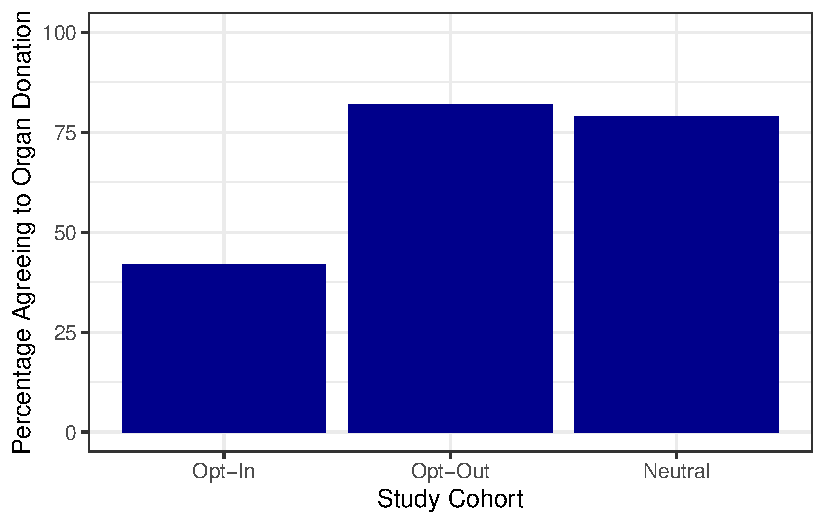
\includegraphics[width=0.8\textwidth,height=\textheight]{./images/fig-basics-organ-plot-1.pdf}

}

\caption{\label{fig-basics-organ-plot}Summary of the responses for the
Organ Donation Study described in
Example~\ref{exm-basics-organ-donation}.}

\end{figure}

\hypertarget{overview-of-drawing-inference}{%
\section{Overview of Drawing
Inference}\label{overview-of-drawing-inference}}

Let's begin by taking a step back and considering the big picture of how
data is turned into information. Every research question we pose, at its
heart, is trying to characterize a \textbf{population}, the group of
subjects of ultimate interest.

\begin{definition}[Population]\protect\hypertarget{def-population}{}\label{def-population}

The collection of subjects we would like to say something about.

\end{definition}

In the Organ Donation study (Example~\ref{exm-basics-organ-donation}),
the researchers would like to say something about Americans who are of
the age to consent to organ donation; in particular, they would like to
quantify how likely it is that someone from this group agrees to organ
donation. Therefore, the population is \emph{all Americans who are of
the age to consent to organ donation}.

In general, the subjects (or units of observation) in a population need
not be people; in some studies, the population could be a collection of
screws, cell phones, sheet metal\ldots whatever characterizes the
objects from which we would \emph{like to} obtain measurements. We use
the phrase ``like to'' because in reality it is often impossible (or
impractical) to observe the entire population. Instead, we make
observations on a subset of the population; this smaller group is known
as the \textbf{sample}.

\begin{definition}[Sample]\protect\hypertarget{def-sample}{}\label{def-sample}

The collection of subjects for which we actually obtain measurements
(data).

\end{definition}

\begin{tcolorbox}[enhanced jigsaw, leftrule=.75mm, coltitle=black, left=2mm, title=\textcolor{quarto-callout-note-color}{\faInfo}\hspace{0.5em}{Note}, breakable, toptitle=1mm, bottomtitle=1mm, colback=white, colbacktitle=quarto-callout-note-color!10!white, titlerule=0mm, opacitybacktitle=0.6, colframe=quarto-callout-note-color-frame, bottomrule=.15mm, arc=.35mm, opacityback=0, rightrule=.15mm, toprule=.15mm]

Some readers may associate ``subjects'' with people; to avoid this
confusion, you may prefer ``unit of observation'' to subject. In this
text, we use subject to mean any unit on which observations could be
taken.

\end{tcolorbox}

For each subject within the sample, we obtain a collection of
measurements forming our set of data. The goal of statistical modeling
is to use the sample (the group we actually observe) to say something
about the population of interest (the group we wish we had observed);
this process is known as \textbf{statistical inference} (illustrated in
Figure~\ref{fig-basics-statistical-process}).

\begin{definition}[Statistical
Inference]\protect\hypertarget{def-inference}{}\label{def-inference}

The process of using a sample to characterize some aspect of the
underlying population.

\end{definition}

\begin{figure}

{\centering 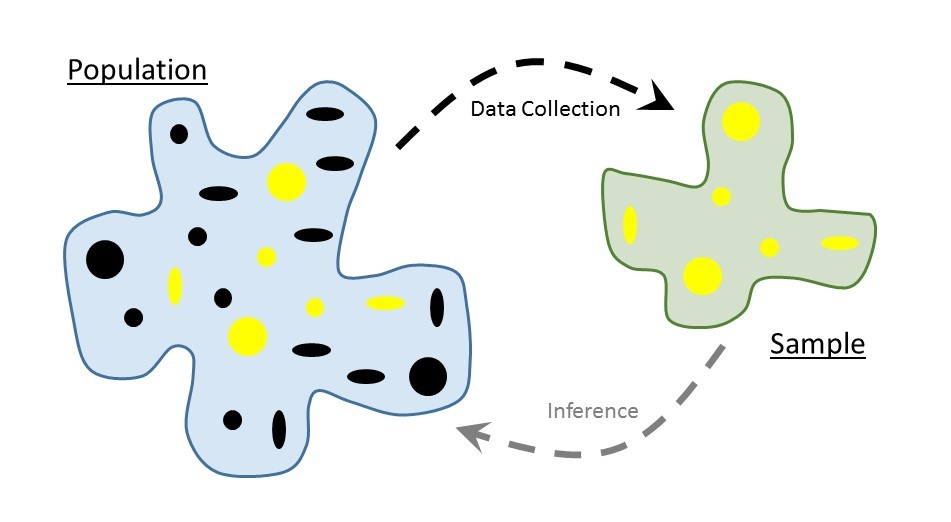
\includegraphics[width=0.8\textwidth,height=\textheight]{images/Basics-Stat-Process.jpg}

}

\caption{\label{fig-basics-statistical-process}Illustration of the
statistical process, using a sample to characterize some aspect of the
underlying population.}

\end{figure}

\hypertarget{anatomy-of-a-dataset}{%
\section{Anatomy of a Dataset}\label{anatomy-of-a-dataset}}

Once we have our sample, we take measurements on each of the subjects
within this sample. These measurements form the data. When we hear the
word ``data,'' most of us envision a large spreadsheet. In reality, data
can take on many forms --- spreadsheets, images, text files,
unstructured text from a social media feed, etc. Regardless of the form,
all datasets contain information for each subject in the sample; this
information, the various measurements, are called \textbf{variables}.

\begin{definition}[Variable]\protect\hypertarget{def-variable}{}\label{def-variable}

A measurement, or category, describing some aspect of the subject.

\end{definition}

Variables come in one of two flavors. \textbf{Categorical} variables are
those which denote a grouping to which the subject belongs. Examples
include marital status, manufacturer, and experimental treatment group.
\textbf{Numeric} variables are those which take on values for which
ordinary arithmetic (e.g., addition and multiplication) makes sense.
Examples include height, age of a product, and diameter. Note that
sometimes numeric values are used to represent the levels of a
categorical variable in a dataset; for example, 0 may indicate ``No''
and 1 may indicate ``Yes'' for a variable capturing whether a person is
a registered organ donor. Therefore, just because a variable has a
numeric value does not make it a numeric variable; the key here is that
numeric variables are those for which arithmetic makes sense.

\begin{definition}[Categorical
Variable]\protect\hypertarget{def-categorical}{}\label{def-categorical}

Also called a ``qualitative variable,'' a measurement on a subject which
denotes a grouping or categorization.

\end{definition}

\begin{definition}[Numeric
Variable]\protect\hypertarget{def-numeric}{}\label{def-numeric}

Also called a ``quantitative variable,'' a measurement on a subject
which takes on a numeric value \emph{and} for which ordinary arithmetic
makes sense.

\end{definition}

While it may be natural to think of a dataset as a spreadsheet, not all
spreadsheets are created equal.

\begin{tcolorbox}[enhanced jigsaw, leftrule=.75mm, coltitle=black, left=2mm, title=\textcolor{quarto-callout-tip-color}{\faLightbulb}\hspace{0.5em}{Characteristics of Well-Structured Data}, breakable, toptitle=1mm, bottomtitle=1mm, colback=white, colbacktitle=quarto-callout-tip-color!10!white, titlerule=0mm, opacitybacktitle=0.6, colframe=quarto-callout-tip-color-frame, bottomrule=.15mm, arc=.35mm, opacityback=0, rightrule=.15mm, toprule=.15mm]

A well-structured dataset should adhere to the following
characteristics:

\begin{itemize}
\tightlist
\item
  Each column contains a unique variable.
\item
  Each record (row in the dataset) corresponds to a different
  observation of the variables.
\item
  If you have multiple datasets, they should include a column in the
  table that allows them to be linked (subject identifier).
\end{itemize}

\end{tcolorbox}

These characteristics ensure the data is properly formatted for an
analysis. Even unstructured data such as images or text files must be
processed prior to performing a statistical analysis.

\begin{tcolorbox}[enhanced jigsaw, leftrule=.75mm, coltitle=black, left=2mm, title=\textcolor{quarto-callout-warning-color}{\faExclamationTriangle}\hspace{0.5em}{Warning}, breakable, toptitle=1mm, bottomtitle=1mm, colback=white, colbacktitle=quarto-callout-warning-color!10!white, titlerule=0mm, opacitybacktitle=0.6, colframe=quarto-callout-warning-color-frame, bottomrule=.15mm, arc=.35mm, opacityback=0, rightrule=.15mm, toprule=.15mm]

We note the above description eliminates a common method of storing data
in engineering and scientific disciplines --- storing each sample in a
different column.

\end{tcolorbox}

To illustrate the above description, suppose we conduct a study
comparing the lifetime (in hours) of two brands of batteries. We measure
the lifetime of five batteries of Brand A and six of Brand B. It is
common to see a dataset like that in
Table~\ref{tbl-basics-poor-dataset}; the problem here is that the first
record of the dataset contains information on two different units of
observation. We have the lifetime from a battery of Brand A in the same
row as the lifetime from a battery of Brand B. This violates the second
characteristic of datasets described above.

\hypertarget{tbl-basics-poor-dataset}{}
\begin{table}
\caption{\label{tbl-basics-poor-dataset}Example of a common data structure which does not correspond to the
characteristics of well-structured data we recommend. The data is from a
hypothetical study comparing battery lifetimes (hours). }\tabularnewline

\centering
\begin{tabular}[t]{cc}
\toprule
Brand A & Brand B\\
\midrule
\cellcolor{gray!6}{8.3} & \cellcolor{gray!6}{8.4}\\
5.1 & 8.6\\
\cellcolor{gray!6}{3.3} & \cellcolor{gray!6}{3.8}\\
5.3 & 4.1\\
\cellcolor{gray!6}{5.7} & \cellcolor{gray!6}{4.5}\\
\addlinespace
 & 4.0\\
\bottomrule
\end{tabular}
\end{table}

In order to adhere to the characteristics of well-structured data
outlined above, we can reformat the data in
Table~\ref{tbl-basics-poor-dataset} to that shown in
Table~\ref{tbl-basics-good-dataset}. Here, each record represents a
unique observation and each column is a different variable. We have also
added a unique identifier.

\hypertarget{tbl-basics-good-dataset}{}
\begin{table}
\caption{\label{tbl-basics-good-dataset}Example of a well-structured dataset. The data is from a hypothetical
study comparing battery lifetimes (hours). }\tabularnewline

\centering
\begin{tabular}[t]{ccc}
\toprule
Battery & Brand & Lifetime\\
\midrule
\cellcolor{gray!6}{1} & \cellcolor{gray!6}{A} & \cellcolor{gray!6}{8.3}\\
2 & A & 5.1\\
\cellcolor{gray!6}{3} & \cellcolor{gray!6}{A} & \cellcolor{gray!6}{3.3}\\
4 & A & 5.3\\
\cellcolor{gray!6}{5} & \cellcolor{gray!6}{A} & \cellcolor{gray!6}{5.7}\\
\addlinespace
6 & B & 8.4\\
\cellcolor{gray!6}{7} & \cellcolor{gray!6}{B} & \cellcolor{gray!6}{8.6}\\
8 & B & 3.8\\
\cellcolor{gray!6}{9} & \cellcolor{gray!6}{B} & \cellcolor{gray!6}{4.1}\\
10 & B & 4.5\\
\addlinespace
\cellcolor{gray!6}{11} & \cellcolor{gray!6}{B} & \cellcolor{gray!6}{4.0}\\
\bottomrule
\end{tabular}
\end{table}

It may take some time to get used to storing data in this format, but it
makes analysis easier and avoids time spent managing the data later.

\hypertarget{a-note-on-codebooks}{%
\section{A Note on Codebooks}\label{a-note-on-codebooks}}

A dataset on its own is meaningless if you cannot understand what the
values represent. \emph{Before} you access a dataset, you should always
review any available \textbf{codebooks}.

\begin{definition}[Codebook]\protect\hypertarget{def-codebook}{}\label{def-codebook}

Also called a ``data dictionary,'' these provide complete information
regarding the variables contained within a dataset.

\end{definition}

Some codebooks are excellent, with detailed descriptions of how the
variables were collected alongside appropriate units for the
measurements. Other codebooks give only an indication of what each
variable represents. Whenever you are working with previously collected
data, reviewing a codebook is the first step; and, you should be
prepared to revisit the codebook often throughout an analysis. When you
are collecting your own dataset, constructing a codebook is essential
for others to make use of your data.

\hypertarget{sec-caseDeepwater}{%
\chapter{Case Study: Health Effects of the Deepwater Horizon Oil
Spill}\label{sec-caseDeepwater}}

\providecommand{\norm}[1]{\lVert#1\rVert}
\providecommand{\abs}[1]{\lvert#1\rvert}
\providecommand{\iid}{\stackrel{\text{IID}}{\sim}}
\providecommand{\ind}{\stackrel{\text{Ind}}{\sim}}

\providecommand{\bm}[1]{\mathbf{#1}}
\providecommand{\bs}[1]{\boldsymbol{#1}}
\providecommand{\bbeta}{\bs{\beta}}

\providecommand{\Ell}{\mathcal{L}}
\providecommand{\indep}{\perp\negthickspace\negmedspace\perp}

On the evening of April 20, 2010, the \emph{Deepwater Horizon}, an oil
drilling platform positioned off the coast of Louisiana, was engulfed in
flames as the result of an explosion. The drilling rig, leased and
operated by BP, had been tasked with drilling an oil well in water
nearly 5000 feet deep. Eleven personnel were killed in the explosion.
The following screenshot is from the initial coverage by the \emph{New
York Times}\footnote{\url{http://www.nytimes.com/2010/04/22/us/22rig.html?rref=collection\%2Ftimestopic\%2FOil\%20Spills\&action=click\&contentCollection=timestopics\&region=stream\&module=stream_unit\&version=search\&contentPlacement=1\&pgtype=collection}}:

\begin{figure}

{\centering 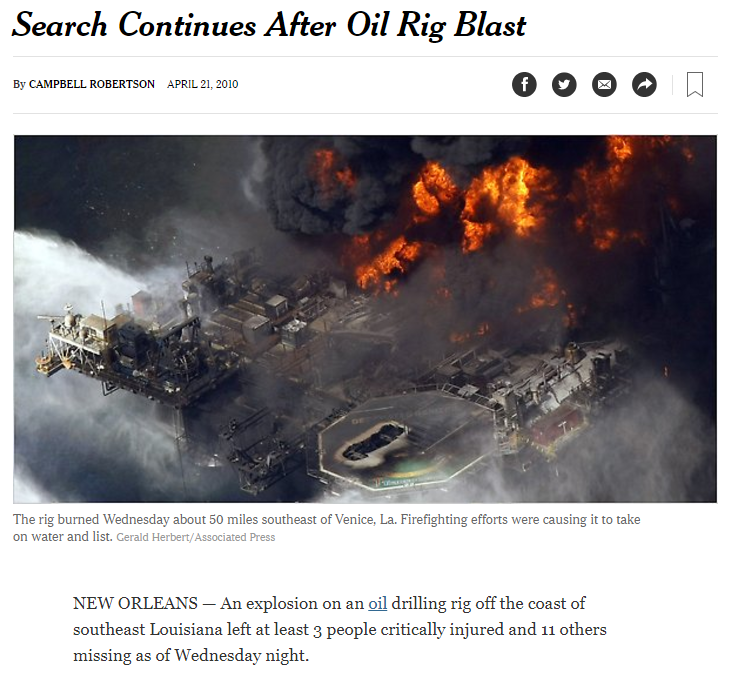
\includegraphics[width=0.8\textwidth,height=\textheight]{./images/Case-Deepwater-NYTclip.png}

}

\caption{\label{fig-casedeepwater-nytclip}\emph{New York Times} coverage
of the \emph{Deepwater Horizon} oil spill.}

\end{figure}

The incident is considered the worst oil spill in US history, creating
an environmental disaster along the Gulf Coast. In addition to studying
the effects on the local environment, researchers have undertaken
studies to examine the short and long-term health effects caused by the
incident. As an example, we might ask whether volunteers who were
directly exposed to oil, such as when cleaning wildlife, are at higher
risk of respiratory irritation compared to those volunteers who were
helping with administrative tasks (and therefore were not directly
exposed to oil). An article appearing in \emph{The New England Journal
of Medicine} (Goldstein, Osofsky, and Lichtveld 2011) reported the
results from a health symptom survey performed in the Spring and Summer
of 2010 by the National Institute for Occupational Safety and Health. Of
54 volunteers assigned to wildlife cleaning and rehabilitation, 15
reported experiencing ``nose irritation, sinus problems, or sore
throat.'' Of 103 volunteers who had no exposure to oil, dispersants,
cleaners, or other chemicals, 16 reported experiencing ``nose
irritation, sinus problems, or sore throat.''

While a larger fraction of volunteers cleaning wildlife \emph{in the
study} reported respiratory symptoms compared to those who were not
directly exposed to irritants, would we expect similar results if we
were able to interview all volunteers? What about during a future oil
spill? Is there evidence that more than 1 in 5 volunteers who clean
wildlife will develop respiratory symptoms? What is a reasonable value
for the increased risk of respiratory symptoms for those volunteers with
direct exposure compared to those without?

In the first part of this text, we use this motivating example as the
context for discussing how research questions should be framed, methods
for data collection, summarizing and presenting data clearly,
quantifying the variability in an estimate, and quantifying the degree
to which the data disagrees with a proposed model. We capture these
ideas in what we call the \emph{Five Fundamental Ideas of Inference}. We
will also see that any statistical analysis moves between the components
of what we call the \emph{Distributional Quartet}. These two frameworks
allow us to describe the language and logic of inference, serving as a
foundation for the statistical thinking and reasoning needed to address
more complex questions encountered later in the text.

\hypertarget{sec-questions}{%
\chapter{Asking the Right Questions}\label{sec-questions}}

\providecommand{\norm}[1]{\lVert#1\rVert}
\providecommand{\abs}[1]{\lvert#1\rvert}
\providecommand{\iid}{\stackrel{\text{IID}}{\sim}}
\providecommand{\ind}{\stackrel{\text{Ind}}{\sim}}

\providecommand{\bm}[1]{\mathbf{#1}}
\providecommand{\bs}[1]{\boldsymbol{#1}}
\providecommand{\bbeta}{\bs{\beta}}

\providecommand{\Ell}{\mathcal{L}}
\providecommand{\indep}{\perp\negthickspace\negmedspace\perp}

The discipline of statistics is about turning data into information in
order to address some question. While there may be no such thing as a
stupid question, there are ill-posed questions --- those which cannot be
answered as stated. Consider the
\protect\hyperlink{sec-caseDeepwater}{Deepwater Horizon Case Study}
(Chapter~\ref{sec-caseDeepwater}). It might seem natural to ask ``if a
volunteer cleans wildlife, will she develop adverse respiratory
symptoms?'' Let's consider the data. Of the 54 volunteers assigned to
wildlife cleaning and rehabilitation, 15 reported experiencing adverse
respiratory symptoms (``nose irritation, sinus problems, or sore
throat''); while some volunteers developed symptoms, others did not. It
seems the answer to our question is then ``it depends'' or ``maybe.''
This is an example of an \emph{ill-posed question}. Such questions exist
because of \textbf{variability}, the fact that every subject in the
population does not behave in exactly the same way; that is, the value
of a variable potentially differs from one observation to the next. In
our example not every volunteer had the same reaction when directly
exposed to oil.

It is variability that creates a need for the discipline of statistics;
in fact, you could think of statistics as the study and characterization
of variability. We must therefore learn to ask the \emph{right}
questions --- those which can be answered in the presence of
variability.

\begin{definition}[Variability]\protect\hypertarget{def-variability}{}\label{def-variability}

The notion that measurements differ from one observation to another.

\end{definition}

\begin{tcolorbox}[enhanced jigsaw, leftrule=.75mm, coltitle=black, left=2mm, title=\textcolor{quarto-callout-tip-color}{\faLightbulb}\hspace{0.5em}{Big Idea}, breakable, toptitle=1mm, bottomtitle=1mm, colback=white, colbacktitle=quarto-callout-tip-color!10!white, titlerule=0mm, opacitybacktitle=0.6, colframe=quarto-callout-tip-color-frame, bottomrule=.15mm, arc=.35mm, opacityback=0, rightrule=.15mm, toprule=.15mm]

The presence of variability makes some questions ill-posed; statistics
concerns itself with how to address questions in the presence of
variability.

\end{tcolorbox}

\hypertarget{characterizing-a-variable}{%
\section{Characterizing a Variable}\label{characterizing-a-variable}}

Recall that the goal of statistical inference is to say something about
the population; as a result, any question we ask should then be about on
this larger group. The first step to constructing a well-posed question
is then to identify the population of interest for the study. For the
\protect\hyperlink{sec-caseDeepwater}{Deepwater Horizon Case Study}, it
is unlikely that we are only interested in these 54 observed volunteers
assigned to wildlife cleaning. In reality, we probably want to say
something about volunteers for any oil spill. The 54 volunteers in our
dataset form the sample, a subset from all volunteers who clean wildlife
following an oil spill. Our population of interest is comprised of all
volunteers who clean wildlife following an oil spill.

\begin{tcolorbox}[enhanced jigsaw, leftrule=.75mm, coltitle=black, left=2mm, title=\textcolor{quarto-callout-note-color}{\faInfo}\hspace{0.5em}{Note}, breakable, toptitle=1mm, bottomtitle=1mm, colback=white, colbacktitle=quarto-callout-note-color!10!white, titlerule=0mm, opacitybacktitle=0.6, colframe=quarto-callout-note-color-frame, bottomrule=.15mm, arc=.35mm, opacityback=0, rightrule=.15mm, toprule=.15mm]

When identifying the population of interest for a research question you
have, be specific! Suppose you are trying to estimate the average height
of trees. Are you really interested in \emph{all} trees? Or, are you
interested in Maple trees within the city limits of Terre Haute,
Indiana?

\end{tcolorbox}

Since we expect that the reaction to oil exposure --- the primary
variable of interest for this study, sometimes called the
\textbf{response} --- to vary from one individual to another, we cannot
ask a question about the \emph{value} of the reaction (whether they
experienced symptoms or not). Instead, we want to characterize the
\textbf{distribution} of the response.

\begin{definition}[Response]\protect\hypertarget{def-response}{}\label{def-response}

The primary variable of interest within a study. This is the variable
you would either like to explain or estimate.

\end{definition}

\begin{definition}[Distribution]\protect\hypertarget{def-distribution}{}\label{def-distribution}

The pattern of variability corresponding to a set of values.

\end{definition}

Notice that in this case, the response is a categorical variable;
describing the distribution of such a variable is equivalent to
describing how individuals are divided among the possible groups. With a
finite number of observations, we could present the number of
observations, the \textbf{frequency}, within each group. For example, of
the 54 volunteers, 15 experienced adverse symptoms and 39 did not. This
works well within the sample; however, as our population is infinitely
large (all volunteers cleaning wildlife following an oil spill),
reporting the frequencies is not appropriate. In this case, we report
the fraction of observations, the \textbf{relative frequency}, falling
within each group; this helps convey information about the distribution
of this variable. That is, the relative frequencies give us a sense of
which values of the variable are more or less common in the sample.

\begin{definition}[Frequency]\protect\hypertarget{def-frequency}{}\label{def-frequency}

The number of observations in a sample falling into a particular group
(level) defined by a categorical variable.

\end{definition}

\begin{definition}[Relative
Frequency]\protect\hypertarget{def-relative-frequency}{}\label{def-relative-frequency}

Also called the ``proportion,'' the fraction of observations falling
into a particular group (level) of a categorical variable.

\end{definition}

Numeric quantities, like the proportion, which summarize the
distribution of a variable within the population are known as
\textbf{parameters}.

\begin{definition}[Parameter]\protect\hypertarget{def-parameter}{}\label{def-parameter}

Numeric quantity which summarizes the distribution of a variable within
the \emph{population} of interest. Generally denoted by Greek letters in
statistical formulas.

\end{definition}

While the \emph{value} of a variable may vary across the population, the
\emph{parameter} is a single fixed constant which summarizes the
variable for that population. For example, the grade received on an exam
varies from one student to another in a class; but, the \emph{average
exam grade} is a fixed number which summarizes the class as a whole.
Well-posed questions can be constructed if we limit ourselves to
questions about the parameter. The second step in constructing
well-posed questions is then to identify the parameter of interest.

The questions we ask generally fall into one of two categories:

\begin{itemize}
\tightlist
\item
  Estimation: what \emph{proportion} of volunteers who clean wildlife
  following an oil spill will experience adverse respiratory symptoms?
\item
  Hypothesis Testing: is it reasonable no more than 1 in 5 volunteers
  who clean wildlife following an oil spill will experience adverse
  respiratory symptoms; or, is there evidence more than 1 in 5
  volunteers who clean wildlife following an oil spill will experience
  adverse respiratory symptoms?
\end{itemize}

\begin{definition}[Estimation]\protect\hypertarget{def-estimation}{}\label{def-estimation}

Using the sample to approximate the value of a parameter from the
underlying population.

\end{definition}

\begin{definition}[Hypothesis
Testing]\protect\hypertarget{def-hypothesis-testing}{}\label{def-hypothesis-testing}

Using a sample to determine if the data is consistent with a working
theory or if there is evidence to suggest the data is not consistent
with the theory.

\end{definition}

Since we do not get to observe the population (we only see the sample),
we cannot observe the value of the parameter. That is, we will never
know the true proportion of volunteers who experience symptoms. However,
we can determine what the data suggests about the population (that is
what inference is all about).

\begin{tcolorbox}[enhanced jigsaw, leftrule=.75mm, coltitle=black, left=2mm, title=\textcolor{quarto-callout-tip-color}{\faLightbulb}\hspace{0.5em}{Big Idea}, breakable, toptitle=1mm, bottomtitle=1mm, colback=white, colbacktitle=quarto-callout-tip-color!10!white, titlerule=0mm, opacitybacktitle=0.6, colframe=quarto-callout-tip-color-frame, bottomrule=.15mm, arc=.35mm, opacityback=0, rightrule=.15mm, toprule=.15mm]

Parameters are unknown values and can never, in general, be known.

\end{tcolorbox}

It turns out, the vast majority of research questions can be framed in
terms of a parameter. This is the first of what we consider the
\emph{Five Fundamental Ideas of Inference}.

\begin{tcolorbox}[enhanced jigsaw, leftrule=.75mm, coltitle=black, left=2mm, title=\textcolor{quarto-callout-important-color}{\faExclamation}\hspace{0.5em}{Fundamental Idea I}, breakable, toptitle=1mm, bottomtitle=1mm, colback=white, colbacktitle=quarto-callout-important-color!10!white, titlerule=0mm, opacitybacktitle=0.6, colframe=quarto-callout-important-color-frame, bottomrule=.15mm, arc=.35mm, opacityback=0, rightrule=.15mm, toprule=.15mm]

A research question can often be framed in terms of a parameter that
characterizes the population. Framing the question should then guide our
analysis.

\end{tcolorbox}

We now have a way of describing a well-posed question, a question which
can be addressed using data. Well posed questions are about the
population and can be framed in terms of a parameter which summarizes
that population. We now describe how these questions are typically
framed.

\hypertarget{framing-the-question}{%
\section{Framing the Question}\label{framing-the-question}}

In engineering and scientific applications, many questions fall under
the second category of \textbf{hypothesis testing}, which is a form of
model comparison in which data is collected to help the researcher
choose between two competing theories for the parameter of interest. In
this section, we consider the terminology surrounding specifying such
questions.

For the \protect\hyperlink{sec-caseDeepwater}{Deepwater Horizon Case
Study} suppose we are interested in addressing the following question:

\begin{quote}
Is there evidence that more than 1 in 5 volunteers who clean wildlife
following an oil spill will develop adverse respiratory symptoms?
\end{quote}

The question itself is about the population (all volunteers assigned to
clean wildlife following an oil spill) and is centered on a parameter
(the proportion who develop adverse respiratory symptoms). That is, this
is a well-posed question that can be answered with appropriate data. The
overall process for addressing these types of questions is similar to
conducting a trial in a court of law. In the United States, a trial has
the following essential steps:

\begin{enumerate}
\def\labelenumi{\arabic{enumi}.}
\tightlist
\item
  Assume the defendant is innocent.
\item
  Present evidence to establish guilt, to the contrary of innocence
  (prosecution's responsibility).
\item
  Consider the weight of the evidence presented (jury's responsibility).
\item
  Make a decision. If the evidence is ``beyond a reasonable doubt,'' the
  jury declares the defendant guilty; otherwise, the jury declares the
  defendant not guilty.
\end{enumerate}

The process of conducting a hypothesis test has similar essential steps:

\begin{enumerate}
\def\labelenumi{\arabic{enumi}.}
\tightlist
\item
  Assume the opposite of what we want the data to show (develop a
  working theory).
\item
  Gather data and compare it to the proposed model from step (1).
\item
  Quantify the likelihood of our data from step (2) under the proposed
  model.
\item
  If the likelihood is small, conclude the data is not consistent with
  the working model (there is evidence for what we want to show);
  otherwise, conclude the data is consistent with the working model
  (there is no evidence for what we want to show).
\end{enumerate}

Notice that a trial focuses not on proving guilt but on disproving
innocence; similarly, in statistics, we are able to establish evidence
\emph{against} a specified theory. This is one of several subtle points
in hypothesis testing. We will discuss these subtleties at various
points throughout the text and revisit the overall concepts often. Here,
we focus solely on that first step --- developing a working theory that
we want to \emph{disprove}.

\begin{tcolorbox}[enhanced jigsaw, leftrule=.75mm, coltitle=black, left=2mm, title=\textcolor{quarto-callout-note-color}{\faInfo}\hspace{0.5em}{Note}, breakable, toptitle=1mm, bottomtitle=1mm, colback=white, colbacktitle=quarto-callout-note-color!10!white, titlerule=0mm, opacitybacktitle=0.6, colframe=quarto-callout-note-color-frame, bottomrule=.15mm, arc=.35mm, opacityback=0, rightrule=.15mm, toprule=.15mm]

This process may seem counter-intuitive; it is natural to ask ``why
can't we prove guilt directly?'' However, when you disprove one
statement, you are proving that statement's opposite --- a technique
known in mathematics as ``proof by contradiction.'' So, our approach to
proving a statement is to disprove all other possibilities. It is
similar to the technique of the fictional detective Sherlock Holmes
(Doyle 1890, pg. 92): ``Eliminate all other factors, and the one which
remains must be the truth.''

\end{tcolorbox}

Consider the above question for the
\protect\hyperlink{sec-caseDeepwater}{Deepwater Horizon Case Study}. We
want to find evidence that the proportion experiencing adverse symptoms
exceeds 0.20 (1 in 5). Therefore, we would like to \emph{disprove} (or
provide evidence \emph{against}) the statement that the proportion
experiencing adverse symptoms is no more than 0.20. This statement that
we would like to disprove is known as the \textbf{null hypothesis}; the
opposite of this statement, called the \textbf{alternative hypothesis},
captures what we as the researchers would like to establish.

\begin{definition}[Null
Hypothesis]\protect\hypertarget{def-null-hypothesis}{}\label{def-null-hypothesis}

The statement (or theory) about the parameter that we would like to
\emph{disprove}. This is denoted \(H_0\), read ``H-naught'' or
``H-zero''.

\end{definition}

\begin{definition}[Alternative
Hypothesis]\protect\hypertarget{def-alternative-hypothesis}{}\label{def-alternative-hypothesis}

The statement (or theory) about the parameter capturing what we would
like to provide evidence \emph{for}; this is the opposite of the null
hypothesis. This is denoted \(H_1\) or \(H_a\), read ``H-one'' and
``H-A'' respectively.

\end{definition}

For the \protect\hyperlink{sec-caseDeepwater}{Deepwater Horizon Case
Study}, we write:

\begin{quote}
\(H_0:\) The proportion of volunteers assigned to clean wildlife
following an oil spill who experience adverse respiratory symptoms is no
more than 0.20.\\
\(H_1:\) The proportion of volunteers assigned to clean wildlife
following an oil spill who experience adverse respiratory symptoms
exceeds 0.20.
\end{quote}

Each hypothesis is a well-posed statement (about a parameter
characterizing the entire population), and the two statements are
exactly opposite of one another meaning only one can be a true
statement.

\begin{tcolorbox}[enhanced jigsaw, leftrule=.75mm, coltitle=black, left=2mm, title=\textcolor{quarto-callout-note-color}{\faInfo}\hspace{0.5em}{Note}, breakable, toptitle=1mm, bottomtitle=1mm, colback=white, colbacktitle=quarto-callout-note-color!10!white, titlerule=0mm, opacitybacktitle=0.6, colframe=quarto-callout-note-color-frame, bottomrule=.15mm, arc=.35mm, opacityback=0, rightrule=.15mm, toprule=.15mm]

When framing your questions, be sure your null hypothesis and
alternative hypothesis are exact opposites of one another, and ensure
the ``equality'' component \emph{always} goes in the null hypothesis.

\end{tcolorbox}

We can now collect data and determine if it is \emph{consistent} with
the null hypothesis (a statement similar to ``not guilty'') or if the
data provides \emph{evidence} against the null hypothesis and in favor
of the alternative (a statement similar to ``guilty'').

\begin{tcolorbox}[enhanced jigsaw, leftrule=.75mm, coltitle=black, left=2mm, title=\textcolor{quarto-callout-warning-color}{\faExclamationTriangle}\hspace{0.5em}{Consistent vs.~Evidence}, breakable, toptitle=1mm, bottomtitle=1mm, colback=white, colbacktitle=quarto-callout-warning-color!10!white, titlerule=0mm, opacitybacktitle=0.6, colframe=quarto-callout-warning-color-frame, bottomrule=.15mm, arc=.35mm, opacityback=0, rightrule=.15mm, toprule=.15mm]

The term ``consistent'' and ``reasonable'' will be used interchangeably
throughout the text; however, these terms differ substantially from the
term ``evidence,'' particularly in the Frequentist perspective The data
is said to be consistent with a statement if the data is aligned with
that statement. In general, evidence is a stronger statement.

\end{tcolorbox}

Often these statements are written in a bit more of a mathematical
structure in which a Greek letter is used to represent the parameter of
interest. For example, we might write

\begin{quote}
Let \(\theta\) represent the proportion of volunteers (assigned to clean
wildlife following an oil spill) who experience adverse respiratory
symptoms.\\
\(H_0: \theta \leq 0.20\)\\
\(H_1: \theta > 0.20\)
\end{quote}

In the above statements, \(\theta\) represents the parameter of
interest; the value 0.20 is known as the \textbf{null value}.

\begin{definition}[Null
Value]\protect\hypertarget{def-null-value}{}\label{def-null-value}

The value associated with the equality component of the null hypothesis;
it forms the threshold or boundary between the hypotheses. Note: not all
questions of interest require a null value be specified.

\end{definition}

\begin{tcolorbox}[enhanced jigsaw, leftrule=.75mm, coltitle=black, left=2mm, title=\textcolor{quarto-callout-tip-color}{\faLightbulb}\hspace{0.5em}{Big Idea}, breakable, toptitle=1mm, bottomtitle=1mm, colback=white, colbacktitle=quarto-callout-tip-color!10!white, titlerule=0mm, opacitybacktitle=0.6, colframe=quarto-callout-tip-color-frame, bottomrule=.15mm, arc=.35mm, opacityback=0, rightrule=.15mm, toprule=.15mm]

Hypothesis testing is a form of statistical inference in which we
quantify the evidence \emph{against} a working theory (captured by the
null hypothesis). We essentially argue that the data supports the
alternative if it is not consistent with the working theory.

\end{tcolorbox}

This section has focused on developing the null and alternative
hypothesis when our question of interest is best characterized as one of
comparing models or evaluating a particular statement. If our goal is
estimation, a null and alternative hypothesis are not applicable. For
example, we might have the following goal:

\begin{quote}
Estimate the proportion of volunteers (assigned to clean wildlife
following an oil spill) who experience adverse respiratory symptoms.
\end{quote}

In this version of our research ``question'' there is no statement which
needs to be evaluated. We are interested in estimation, not hypothesis
testing and thus there is no corresponding null and alternative
hypothesis.

\begin{tcolorbox}[enhanced jigsaw, leftrule=.75mm, coltitle=black, left=2mm, title=\textcolor{quarto-callout-note-color}{\faInfo}\hspace{0.5em}{Process for Framing a Question}, breakable, toptitle=1mm, bottomtitle=1mm, colback=white, colbacktitle=quarto-callout-note-color!10!white, titlerule=0mm, opacitybacktitle=0.6, colframe=quarto-callout-note-color-frame, bottomrule=.15mm, arc=.35mm, opacityback=0, rightrule=.15mm, toprule=.15mm]

In order to frame a research question, consider the following steps:

\begin{enumerate}
\def\labelenumi{\arabic{enumi}.}
\tightlist
\item
  Identify the population of interest.\\
\item
  Identify the parameter(s) of interest.
\item
  Determine if you are interested in estimating the parameter(s) or
  quantifying the evidence against some working theory.\\
\item
  If you are interested in testing a working theory, make the null
  hypothesis the working theory and the alternative hypothesis the exact
  opposite statement (capturing what you want to provide evidence for).
\end{enumerate}

\end{tcolorbox}

\hypertarget{sec-data}{%
\chapter{Gathering the Evidence (Data Collection)}\label{sec-data}}

\providecommand{\norm}[1]{\lVert#1\rVert}
\providecommand{\abs}[1]{\lvert#1\rvert}
\providecommand{\iid}{\stackrel{\text{IID}}{\sim}}
\providecommand{\ind}{\stackrel{\text{Ind}}{\sim}}

\providecommand{\bm}[1]{\mathbf{#1}}
\providecommand{\bs}[1]{\boldsymbol{#1}}
\providecommand{\bbeta}{\bs{\beta}}

\providecommand{\Ell}{\mathcal{L}}
\providecommand{\indep}{\perp\negthickspace\negmedspace\perp}

Consider again the goal of statistical inference --- to use a sample as
a snapshot to say something about the underlying population (see
Figure~\ref{fig-data-statistical-process}). This generally provokes
unease in people, leading to a distrust of statistical results. In this
section we attack that distrust head on.

\begin{figure}

{\centering 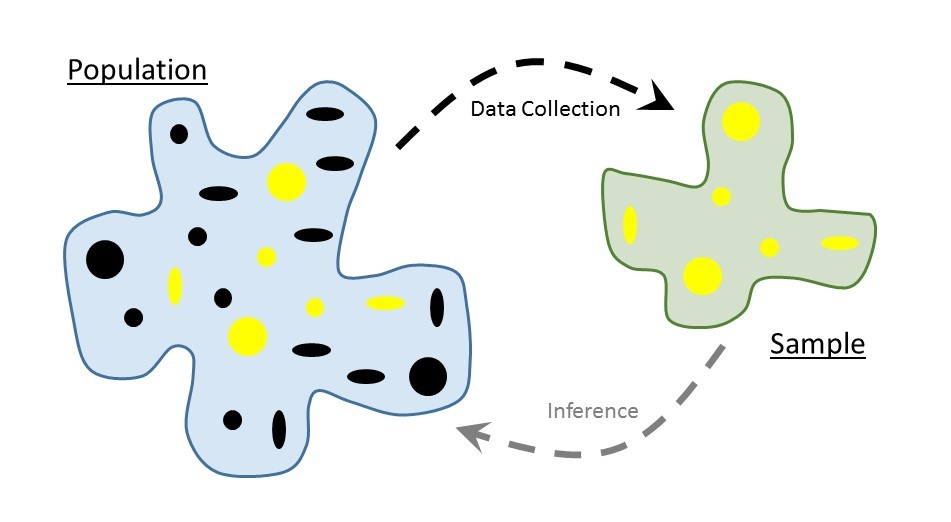
\includegraphics[width=0.8\textwidth,height=\textheight]{images/Basics-Stat-Process.jpg}

}

\caption{\label{fig-data-statistical-process}Illustration of the
statistical process (reprint of
Figure~\ref{fig-basics-statistical-process}).}

\end{figure}

\hypertarget{what-makes-a-sample-reliable}{%
\section{What Makes a Sample
Reliable}\label{what-makes-a-sample-reliable}}

If we are going to have some amount of faith in the statistical results
we produce, we must have data in which we can place our trust. \emph{The
Treachery of Images} (Figure~\ref{fig-data-pipe-img}) is a canvas
painting depicting a pipe, below which the artist wrote the French
phrase ``This is not a pipe.'' Regarding the painting, the artist said

\begin{quote}
The famous pipe. How people reproached me for it! And yet, could you
stuff my pipe? No, it's just a representation, is it not? So if I had
written on my picture ``This is a pipe,'' I'd have been lying!
\end{quote}

\begin{figure}

{\centering 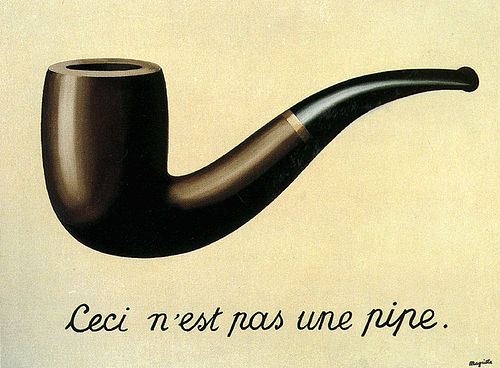
\includegraphics[width=0.8\textwidth,height=\textheight]{./images/Data-Pipe.jpg}

}

\caption{\label{fig-data-pipe-img}\emph{The Treachery of Images} by René
Magritte.}

\end{figure}

Just as a painting is a representation of the object it depicts, so a
sample should be a representation of the population under study. This is
the primary requirement if we are to rely on the resulting data.

\begin{tcolorbox}[enhanced jigsaw, leftrule=.75mm, coltitle=black, left=2mm, title=\textcolor{quarto-callout-tip-color}{\faLightbulb}\hspace{0.5em}{Big Idea}, breakable, toptitle=1mm, bottomtitle=1mm, colback=white, colbacktitle=quarto-callout-tip-color!10!white, titlerule=0mm, opacitybacktitle=0.6, colframe=quarto-callout-tip-color-frame, bottomrule=.15mm, arc=.35mm, opacityback=0, rightrule=.15mm, toprule=.15mm]

In order for a statistical analysis to be reliable, the sample must be
\emph{representative} of the population under study.

\end{tcolorbox}

We need to be careful to not get carried away in our expectations. What
constitutes ``representative'' really depends on the question, just as
an artist chooses their depiction based on how they want to represent
the object. Let's consider the following example.

\begin{example}[School
Debt]\protect\hypertarget{exm-data-school-debt}{}\label{exm-data-school-debt}

In addition to a degree, college graduates also tend to leave with a
large amount of debt due to college loans. In 2012, a graduate with a
student loan had an average debt of \$29,400; for graduates from private
non-profit institutions, the average debt was \$32,300\footnote{http://ticas.org/sites/default/files/pub\_files/Debt\_Facts\_and\_Sources.pdf}.

Suppose we are interested in determining the average amount of debt in
student loans carried by a graduating senior from Rose-Hulman Institute
of Technology, a small private non-profit engineering school. There are
many faculty at Rose-Hulman who choose to send their children to the
institute. Suppose we were to ask 25 such faculty members who have a
child that attended the institute to report the amount of student loans
their children carried upon graduation from Rose-Hulman. Further,
suppose we compile the responses and compute the average amount of debt.
Using the data, we might report that based on our study, there is
significant evidence the average debt carried by a graduate of
Rose-Hulman is far below the \$32,300 reported above (great news for
this year's graduating class)!

Why should we be hesitant to trust the results from our study?

\end{example}

Many objections to statistical results stem from a distrust of whether
the data (the sample) is really representative of the population of
interest. Rose-Hulman, like many other universities, has a policy that
the children of faculty may attend their university (assuming
admittance) tuition-free. We would therefore expect their children to
carry much less debt than the typical graduating senior. There is a
mismatch between the group we would like to study and the data we have
collected.

This example provides a nice backdrop for discussing what it means to be
representative. First, let's define our population; in this case, we are
interested in graduating seniors from Rose-Hulman. The variable of
interest is the amount of debt carried in student loans; the parameter
of interest is then the \emph{average} amount of debt in student loans
carried by graduating seniors of Rose-Hulman. However, the sample
consists of only graduating seniors of Rose-Hulman \emph{who have a
parent employed by the institute}.

With regard to grade point average, the students in our sample are
probably similar to all graduating seniors; the starting salary of the
students in our sample is probably similar to all graduating seniors;
the fraction of mechanical engineering majors versus math majors is
probably similar. So, in many regards the sample is representative of
the population; however, it fails to be representative with regard to
the variable of interest. This is our concern. The amount of debt
carried by students in our sample is not representative of that debt
carried by all graduating seniors from the university.

\begin{tcolorbox}[enhanced jigsaw, leftrule=.75mm, coltitle=black, left=2mm, title=\textcolor{quarto-callout-note-color}{\faInfo}\hspace{0.5em}{Note}, breakable, toptitle=1mm, bottomtitle=1mm, colback=white, colbacktitle=quarto-callout-note-color!10!white, titlerule=0mm, opacitybacktitle=0.6, colframe=quarto-callout-note-color-frame, bottomrule=.15mm, arc=.35mm, opacityback=0, rightrule=.15mm, toprule=.15mm]

When thinking about whether a sample is representative, focus your
attention to the characteristics specific to your research question or
with regard to how you intend to generalize the results.

\end{tcolorbox}

Does that mean the sample we collected in
Example~\ref{exm-data-school-debt} is useless? Yes and no. The sample
collected cannot be used to answer our initial question of interest
since it is not representative of our population. No statistical method
can fix bad data; statistics adheres to the ``garbage-in, garbage-out''
phenomena. If the data is bad, no analysis will undo that. However,
while the sample cannot be used to answer our initial question, it could
be used to address a different question:

\begin{quote}
What is the average amount of debt in student loans carried by
graduating seniors from Rose-Hulman whose parent is a faculty member at
the institute?
\end{quote}

For this revised question, the sample may indeed be representative. If
we are working with previously collected data, we must consider the
population to which our results will generalize. That is, for what
population is the given sample representative? If we are collecting our
data, we need to be sure we collect data in such a way that the data is
representative of our target population. Let's first look at what
\emph{not} to do.

\hypertarget{poor-methods-of-data-collection}{%
\section{Poor Methods of Data
Collection}\label{poor-methods-of-data-collection}}

Example~\ref{exm-data-school-debt} is an example of a ``convenience
sample,'' when the subjects in the sample are chosen simply due to ease
of collection. Examples include surveying students only in your sorority
when you are interested in all students who are part of a sorority on
campus; taking soil samples from only your city when you are interested
in the soil for the entire state; and, obtaining measurements from only
one brand of phone, because it was the only one you could afford on your
budget, when you are interested in studying all cell phones on the
market. A convenience sample is unlikely to be representative if there
is a relationship between the ease of collection and the variable under
study. This was true in the School Debt example; the relationship of a
student to a faculty member, which is what increased the ease of
collection, was directly related to the amount of debt they carried. As
a result, the resulting sample was not representative of the population.

When conducting a survey with human subjects, it is common to only
illicit responses from volunteers. Such ``volunteer samples'' tend to
draw in those with extreme opinions. Consider product ratings on Amazon.
Individual ratings tend to cluster around 5's and 1's. This is because
those customers who take time to submit a review (which is voluntary)
tend to be those who are really thrilled with their product (and want to
encourage others to purchase it) and those who are really disappointed
with their purchase (and want to encourage others to avoid it). Such
surveys often fail to capture those individuals in the population who
have ``middle of the road'' opinions.

We could not possibly name all the poor methods for collecting a sample;
but, poor methods all share something in common --- it is much more
likely the resulting sample is not representative. Failing to be
representative results in \textbf{biased} estimates of the parameter.

\begin{definition}[Bias]\protect\hypertarget{def-bias}{}\label{def-bias}

A set of measurements is said to be biased if they are
\emph{consistently} too high (or too low). Similarly, an estimate of a
parameter is said to be biased if it is \emph{consistently} too high (or
too low).

\end{definition}

To illustrate the concept of bias, consider shooting at a target as in
Figure~\ref{fig-data-bias}. We can consider the center of our target to
be the parameter we would like to estimate within the population; in
this case, some measure of center. The values in our sample (the strikes
on the target) will vary around the parameter; while we do not expect
any one value to hit the target precisely, a ``representative'' sample
is one in which the values tend to be clustered about the parameter
(unbiased). When the sample is not representative, the values in the
sample tend to cluster off the mark (biased). Notice that to be
unbiased, it may be that not a single value in the sample is perfect,
but aggregated together, they point in the right direction. So, bias is
not about an individual measurement being an ``outlier,'' (more on those
in Chapter~\ref{sec-summaries}) but about \emph{consistently} shooting
in the wrong direction.

\begin{figure}

{\centering 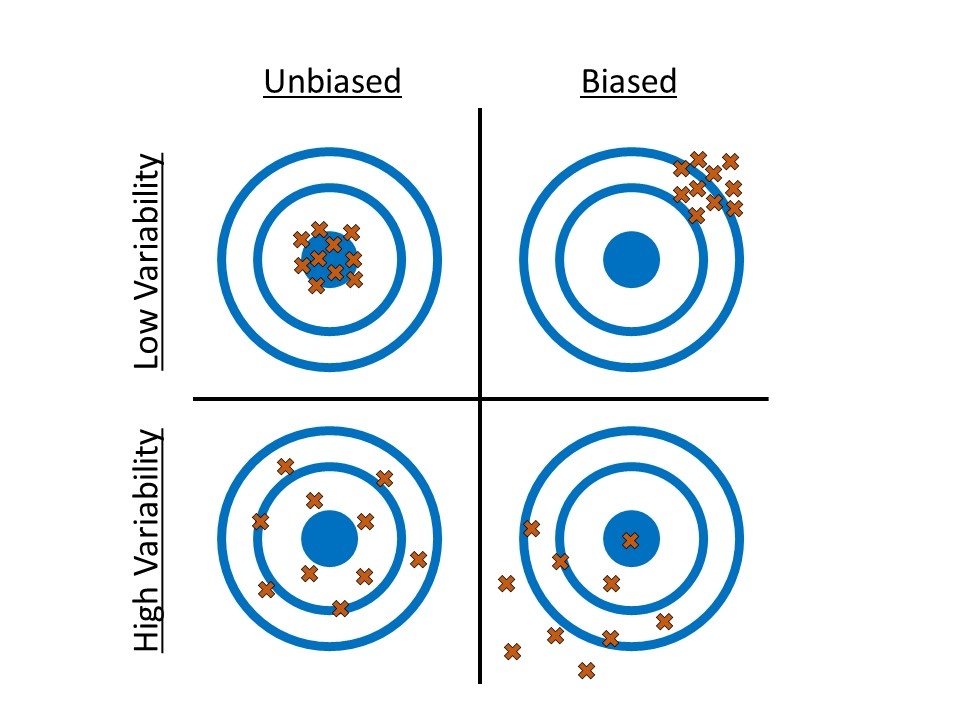
\includegraphics[width=0.8\textwidth,height=\textheight]{./images/Data-Bias.jpg}

}

\caption{\label{fig-data-bias}Illustration of bias and precision.}

\end{figure}

\begin{tcolorbox}[enhanced jigsaw, leftrule=.75mm, coltitle=black, left=2mm, title=\textcolor{quarto-callout-warning-color}{\faExclamationTriangle}\hspace{0.5em}{Accuracy vs.~Precision}, breakable, toptitle=1mm, bottomtitle=1mm, colback=white, colbacktitle=quarto-callout-warning-color!10!white, titlerule=0mm, opacitybacktitle=0.6, colframe=quarto-callout-warning-color-frame, bottomrule=.15mm, arc=.35mm, opacityback=0, rightrule=.15mm, toprule=.15mm]

There is a difference between \emph{accuracy} and \emph{precision}.
Generally, \emph{accuracy} refers to location (and therefore relates to
bias); we say a process is accurate when it is unbiased.
\emph{Precision} refers to the variability; data which is more precise
has less variability.

\end{tcolorbox}

\begin{tcolorbox}[enhanced jigsaw, leftrule=.75mm, coltitle=black, left=2mm, title=\textcolor{quarto-callout-tip-color}{\faLightbulb}\hspace{0.5em}{Big Idea}, breakable, toptitle=1mm, bottomtitle=1mm, colback=white, colbacktitle=quarto-callout-tip-color!10!white, titlerule=0mm, opacitybacktitle=0.6, colframe=quarto-callout-tip-color-frame, bottomrule=.15mm, arc=.35mm, opacityback=0, rightrule=.15mm, toprule=.15mm]

Biased results are typically due to poor sampling methods that result in
a sample which is not representative of the population of interest.

\end{tcolorbox}

The catch (there is always a catch) is that we will never \emph{know}
with certainty if a sample is actually representative or not. In
practice, we critically examine the method in which the sample was
collected, and we use summaries of the sample to make educated decisions
on whether to generalize the results. Better, however, is to employ
methods of data collection that help to minimize the bias in the sample.

\hypertarget{preferred-methods-of-sampling}{%
\section{Preferred Methods of
Sampling}\label{preferred-methods-of-sampling}}

No method guarantees a perfectly representative sample; but, we can take
measures to reduce or eliminate bias. A useful strategy is to employ
\emph{randomization}. This is summarized in our second Fundamental Idea.

\begin{tcolorbox}[enhanced jigsaw, leftrule=.75mm, coltitle=black, left=2mm, title=\textcolor{quarto-callout-important-color}{\faExclamation}\hspace{0.5em}{Fundamental Idea II}, breakable, toptitle=1mm, bottomtitle=1mm, colback=white, colbacktitle=quarto-callout-important-color!10!white, titlerule=0mm, opacitybacktitle=0.6, colframe=quarto-callout-important-color-frame, bottomrule=.15mm, arc=.35mm, opacityback=0, rightrule=.15mm, toprule=.15mm]

If data is to be useful for making conclusions about the population, a
process referred to as drawing inference, proper data collection is
crucial. Randomization can play an important role ensuring a sample is
representative and that inferential conclusions are appropriate.

\end{tcolorbox}

Consider the School Debt example (Example~\ref{exm-data-school-debt})
again. Suppose instead of the data collection strategy described there,
we had done the following:

\begin{quote}
We constructed a list of all graduating seniors from the institute. We
placed the name of each student on an index card; then, we thoroughly
shuffled the cards and chose the top 25 cards. For these 25 individuals,
we recorded the amount of debt in student loans each carried.
\end{quote}

This essentially describes using a lottery to select the sample. This
popular method is known as taking a \textbf{simple random sample}. By
conducting a lottery, we make it very unlikely that our sample consists
of only students with a very small amount of student debt (as occurred
when we used a convenience sample).

\begin{definition}[Simple Random
Sample]\protect\hypertarget{def-simple-random-sample}{}\label{def-simple-random-sample}

Often abbreviated SRS, this is a sample of size \(n\) such that
\emph{every} collection of size \(n\) is equally likely to be the
resulting sample. This is equivalent to a lottery.

\end{definition}

\begin{tcolorbox}[enhanced jigsaw, leftrule=.75mm, coltitle=black, left=2mm, title=\textcolor{quarto-callout-note-color}{\faInfo}\hspace{0.5em}{Note}, breakable, toptitle=1mm, bottomtitle=1mm, colback=white, colbacktitle=quarto-callout-note-color!10!white, titlerule=0mm, opacitybacktitle=0.6, colframe=quarto-callout-note-color-frame, bottomrule=.15mm, arc=.35mm, opacityback=0, rightrule=.15mm, toprule=.15mm]

It is convention to use \(n\) to represent the sample size.

\end{tcolorbox}

The primary benefit of a simple random sample is that it removes bias.
More specifically, the \emph{process} of simple random sampling is
unbiased; that is, this process does \emph{not} produce values which are
\emph{consistently} too high or low.

There are situations in which a simple random sample does not suffice.
Again, consider our School Debt example. The Rose-Hulman student body is
predominantly domestic, with only about 3\% of the student body being
international students. But, suppose we are interested in comparing the
average debt carried between international and domestic students. It is
very likely, by chance alone, that in a simple random sample of 25
students none will be international. Instead of a simple random sample,
we might consider taking a sample of 13 domestic students and a sample
of 12 international students; this is an example of a \textbf{stratified
random sample}. This approach is useful when there is a natural grouping
of interest within the population.

\begin{definition}[Stratified Random
Sample]\protect\hypertarget{def-stratified-random-sample}{}\label{def-stratified-random-sample}

A sample in which the population is first divided into groups, or
strata, based on a characteristic of interest; a simple random sample is
then taken within each group.

\end{definition}

\begin{tcolorbox}[enhanced jigsaw, leftrule=.75mm, coltitle=black, left=2mm, title=\textcolor{quarto-callout-warning-color}{\faExclamationTriangle}\hspace{0.5em}{Warning}, breakable, toptitle=1mm, bottomtitle=1mm, colback=white, colbacktitle=quarto-callout-warning-color!10!white, titlerule=0mm, opacitybacktitle=0.6, colframe=quarto-callout-warning-color-frame, bottomrule=.15mm, arc=.35mm, opacityback=0, rightrule=.15mm, toprule=.15mm]

Note that a stratified random sample essentially results in a
representative sample \emph{within} each strata. However, the combined
sample may not be representative of the population. If there is interest
in using the sample in its entirety, instead of comparing the strata in
some way, advanced statistical methodology is required. See texts on
analyzing ``complex survey design'' for a more thorough discussion. Our
text will not consider such cases.

\end{tcolorbox}

There are countless sampling techniques used in practice. The two
described above can be very useful starting points for developing a
custom method suitable for a particular application. Their benefit stems
from their use of randomization as it limits researcher influence on the
composition of the sample and therefore minimizes bias.

This section is entitled ``Preferred Methods'' because while these
methods are ideal, they are not always practical. Consider the Deepwater
Horizon Case Study described in Chapter~\ref{sec-caseDeepwater};
conceptually, we can take a simple random sample of the volunteers for
our study. However, as with any study involving human subjects,
researchers would be required to obtain consent from each subject in the
study. That is, any individual has the right to refuse to participate in
the study. Therefore, it is unlikely that a simple random sample as
described above could be obtained. While random selection is a nice
tool, the goal is a sample which is \emph{representative} of the
population. While random sampling is helpful for accomplishing this, we
may need to appeal to the composition of the sample itself to justify
its use. \emph{Based on the characteristics of those willing to
participate in the study, do we feel the study participants form a
representative group of all volunteers?} That is the essential question.
This is often why studies report a table summarizing participant
demographics such as age, gender, etc. It is also why it is extremely
important for researchers to describe how observations were obtained so
that readers may make the judgement for themselves whether the sample is
representative.

\hypertarget{sec-summaries}{%
\chapter{Presenting the Evidence (Summarizing
Data)}\label{sec-summaries}}

\providecommand{\norm}[1]{\lVert#1\rVert}
\providecommand{\abs}[1]{\lvert#1\rvert}
\providecommand{\iid}{\stackrel{\text{IID}}{\sim}}
\providecommand{\ind}{\stackrel{\text{Ind}}{\sim}}

\providecommand{\bm}[1]{\mathbf{#1}}
\providecommand{\bs}[1]{\boldsymbol{#1}}
\providecommand{\bbeta}{\bs{\beta}}

\providecommand{\Ell}{\mathcal{L}}
\providecommand{\indep}{\perp\negthickspace\negmedspace\perp}

If you open any search engine and look up ``data visualization,'' you
will quickly be overwhelmed by a host of pages, texts, and software
filled with tools for summarizing your data. Here is the bottom line: a
good visualization is one that helps you answer your question of
interest. It is both that simple and that complicated.

\begin{tcolorbox}[enhanced jigsaw, leftrule=.75mm, coltitle=black, left=2mm, title=\textcolor{quarto-callout-important-color}{\faExclamation}\hspace{0.5em}{Fundamental Idea III}, breakable, toptitle=1mm, bottomtitle=1mm, colback=white, colbacktitle=quarto-callout-important-color!10!white, titlerule=0mm, opacitybacktitle=0.6, colframe=quarto-callout-important-color-frame, bottomrule=.15mm, arc=.35mm, opacityback=0, rightrule=.15mm, toprule=.15mm]

The use of data for decision making requires that the data be summarized
and presented in ways that address the question of interest and
represent the variability present.

\end{tcolorbox}

Whether simple or complex, all graphical and numerical summaries should
help turn the data into usable information. Pretty pictures for the sake
of pretty pictures are not helpful. In this chapter, we will consider
various simple graphical and numerical summaries to help build a case
for addressing the question of interest. The majority of the chapter is
focused on summarizing a single variable; more complex graphics are
presented in future chapters within a context that requires them.

\hypertarget{characteristics-of-a-distribution-summarizing-a-single-variable}{%
\section{Characteristics of a Distribution (Summarizing a Single
Variable)}\label{characteristics-of-a-distribution-summarizing-a-single-variable}}

Remember that because of \emph{variability}, the key to asking good
questions is to not ask questions about individual values but to
characterize the underlying \emph{distribution} (see
Definition~\ref{def-distribution}). Therefore, characterizing the
underlying distribution is also the key to a good visualization or
numeric summary. For the Deepwater Horizon Case Study described in
Chapter~\ref{sec-caseDeepwater}, the response (whether a volunteer
experienced adverse respiratory symptoms) is categorical. As we stated
previously, summarizing the distribution of a categorical variable
reduces to showing the proportion of individual subjects that fall into
each of the various groups defined by the categorical variable.
Figure~\ref{fig-summaries-deepwater-barchart}) displays a \emph{bar
chart} summarizing the rate of respiratory symptoms for volunteers
cleaning wildlife.

\begin{figure}

{\centering 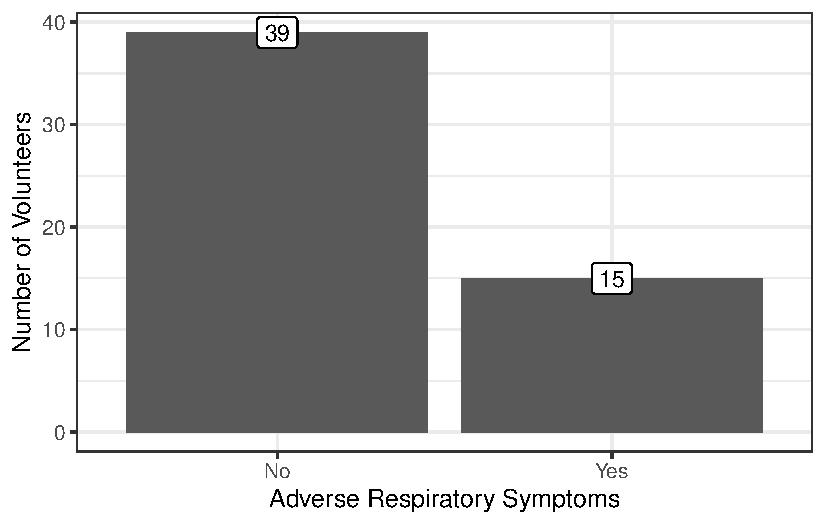
\includegraphics[width=0.8\textwidth,height=\textheight]{./images/fig-summaries-deepwater-barchart-1.pdf}

}

\caption{\label{fig-summaries-deepwater-barchart}Frequency of adverse
respiratory symptoms for volunteers cleaning wildlife following the
Deepwater Horizon oil spill.}

\end{figure}

In general, it does not matter whether the frequency or the relative
frequencies are reported; however, if the relative frequencies are
plotted, some indication of the sample size should be provided with the
figure, either as an annotation or within the caption. From the above
graphic, we see that nearly 28\% of volunteers assigned to wildlife
experienced adverse respiratory symptoms; the graphic helps address our
question, even if not definitively.

\begin{tcolorbox}[enhanced jigsaw, leftrule=.75mm, coltitle=black, left=2mm, title=\textcolor{quarto-callout-note-color}{\faInfo}\hspace{0.5em}{Note}, breakable, toptitle=1mm, bottomtitle=1mm, colback=white, colbacktitle=quarto-callout-note-color!10!white, titlerule=0mm, opacitybacktitle=0.6, colframe=quarto-callout-note-color-frame, bottomrule=.15mm, arc=.35mm, opacityback=0, rightrule=.15mm, toprule=.15mm]

When you are summarizing only categorical variables, a bar chart is
sufficient. Statisticians tend to agree that bar charts are preferable
to pie charts (see
\href{https://www.perceptualedge.com/articles/visual_business_intelligence/save_the_pies_for_dessert.pdf}{this
whitepaper} and
\href{http://www.storytellingwithdata.com/blog/2014/06/alternatives-to-pies}{this
blog} for further explanation).

\end{tcolorbox}

While a single type of graphic (bar charts) are helpful for looking at
categorical data, summarizing the distribution of a numeric variable
requires a bit more thought. Consider the following example.

\begin{example}[Paper
Strength]\protect\hypertarget{exm-summaries-paper}{}\label{exm-summaries-paper}

While electronic records have become the predominant means of storing
information, we do not yet live in a paperless society. Paper products
are still used in a variety of applications ranging from printing
reports and photography to packaging and bathroom tissue. In
manufacturing paper for a particular application, the strength of the
resulting paper product is a key characteristic.

There are several metrics for the strength of paper. A conventional
metric for assessing the inherent (not dependent upon the physical
characteristics, such as the weight of the paper, which might have an
effect) strength of paper is the \emph{breaking length}. This is the
length of a paper strip, if suspended vertically from one end, that
would break under its own weight. Typically reported in kilometers, the
breaking length is computed from other common measurements. For more
information on paper strength measurements and standards, see the
following website: \url{http://www.paperonweb.com}

A study was conducted at the University of Toronto to investigate the
relationship between pulp fiber properties and the resulting paper
properties (Lee 1992). The breaking length was obtained for each of the
62 paper specimens, the first 5 measurements of which are shown in
Table~\ref{tbl-summaries-paper-table}. The complete dataset is available
online at the following website:
\url{https://vincentarelbundock.github.io/Rdatasets/doc/robustbase/pulpfiber.html}

While there are several questions one might ask with the available data,
here we are primarily interested in characterizing the breaking length
of these paper specimens.

\end{example}

\hypertarget{tbl-summaries-paper-table}{}
\begin{table}
\caption{\label{tbl-summaries-paper-table}Breaking length (km) for first 5 specimens in the Paper Strength study. }\tabularnewline

\centering
\begin{tabular}[t]{rr}
\toprule
Specimen & Breaking Length\\
\midrule
\cellcolor{gray!6}{1} & \cellcolor{gray!6}{21.312}\\
2 & 21.206\\
\cellcolor{gray!6}{3} & \cellcolor{gray!6}{20.709}\\
4 & 19.542\\
\cellcolor{gray!6}{5} & \cellcolor{gray!6}{20.449}\\
\bottomrule
\end{tabular}
\end{table}

Figure~\ref{fig-summaries-paper-dotplot} presents the breaking length
for all 62 paper specimens in the sample through a \emph{dot plot} in
which the breaking length for each observed specimen is represented on a
number line using a single dot.

\begin{figure}

{\centering 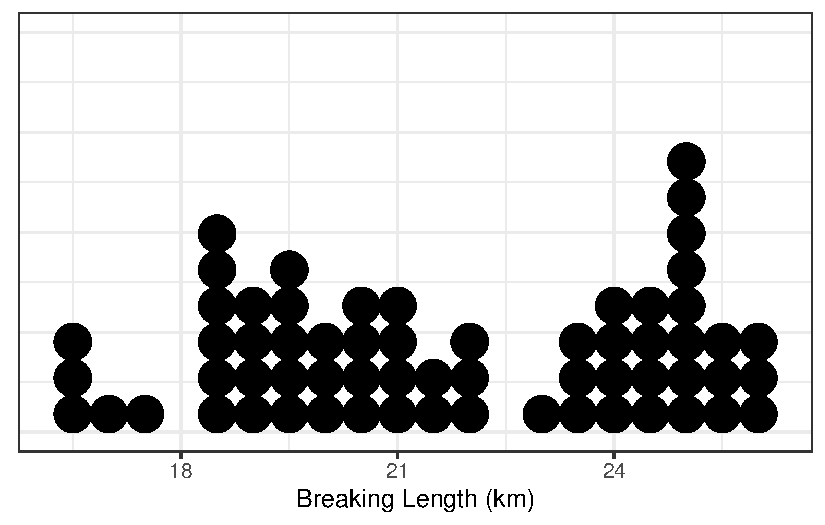
\includegraphics[width=0.8\textwidth,height=\textheight]{./images/fig-summaries-paper-dotplot-1.pdf}

}

\caption{\label{fig-summaries-paper-dotplot}Breaking Length (km) for 62
paper specimens.}

\end{figure}

With any graphic, we tend to be drawn to three components:

\begin{itemize}
\tightlist
\item
  \emph{where} the values tend to be,
\item
  \emph{how tightly} the values tend to be clustered there, and
\item
  \emph{the way} the values tend to cluster.
\end{itemize}

Notice that about half of the paper specimens in the sample had a
breaking length longer than 21.26 km. Only about 25\% of paper specimens
had a breaking length less than 19.33 km. These are measures of
\emph{location}. In particular, these are known as \textbf{percentiles},
of which the \textbf{median}, \textbf{first quartile} and \textbf{third
quartile} are commonly used examples.

\begin{definition}[Percentile]\protect\hypertarget{def-percentile}{}\label{def-percentile}

The \(k\)-th percentile is the value \(q\) such that \(k\)\% of the
values in the distribution are less than or equal to \(q\). For example,

\begin{itemize}
\tightlist
\item
  25\% of values in a distribution are less than or equal to the 25-th
  percentile (known as the ``first quartile'' and denoted \(Q_1\)).
\item
  50\% of values in a distribution are less than or equal to the 50-th
  percentile (known as the ``median'').
\item
  75\% of values in a distribution are less than or equal to the 75-th
  percentile (known as the ``third quartile'' and denoted \(Q_3\)).
\end{itemize}

\end{definition}

The \textbf{average} is also a common measure of location. The breaking
length of a paper specimen is 21.72 km, on average. In this case, the
average breaking length and median breaking length are very close; this
need not be the case. The average is not describing the ``center'' of
the data in the same way as the median; they capture different
properties.

\begin{definition}[Average]\protect\hypertarget{def-average}{}\label{def-average}

Also known as the ``mean,'' this measure of location represents the
balance point for the distribution. If \(x_i\) represents the \(i\)-th
value of the variable \(x\) in the sample, the sample mean is typically
denoted by \(\bar{x}\).

For a sample of size \(n\), it is computed by
\[\bar{x} = \frac{1}{n}\sum_{i=1}^{n} x_i.\]

When referencing the average for a population, the mean is also called
the ``Expected Value,'' and is often denoted by \(\mu\).

\end{definition}

Clearly, the breaking length is not equivalent for all paper specimens;
that is, there is variability in the measurements. Measures of
\emph{spread} quantify the variability of values within a distribution.
Common examples include the \textbf{standard deviation} (related to
\textbf{variance}) and \textbf{interquartile range}. For the Paper
Strength example, the breaking length varies with a standard deviation
of 2.88 km; the interquartile range for the breaking length is 5.2 km.

The standard deviation is often reported more often than the variance
since it is on the same scale as the original data; however, as we will
see later, the variance is useful from a mathematical perspective for
derivations. Neither of these values has a natural interpretation;
instead, larger values of these measures simply indicate a higher degree
of variability in the data.

\begin{definition}[Variance]\protect\hypertarget{def-variance}{}\label{def-variance}

A measure of spread, this roughly captures the average distance values
in the distribution are from the mean.

For a sample of size \(n\), it is computed by
\[s^2 = \frac{1}{n-1}\sum_{i=1}^{n} \left(x_i - \bar{x}\right)^2\]

where \(\bar{x}\) is the sample mean and \(x_i\) is the \(i\)-th value
in the sample. The division by \(n-1\) instead of \(n\) removes bias in
the statistic.

The symbol \(\sigma^2\) is often used to denote the variance in the
population.

\end{definition}

\begin{definition}[Standard
Deviation]\protect\hypertarget{def-standard-deviation}{}\label{def-standard-deviation}

A measure of spread, this is the square root of the variance.

\end{definition}

\begin{definition}[Interquartile
Range]\protect\hypertarget{def-interquartile-range}{}\label{def-interquartile-range}

Often abbreviated as IQR, this is the distance between the first and
third quartiles. This measure of spread indicates the range over which
the middle 50\% of the data is spread.

\end{definition}

\begin{tcolorbox}[enhanced jigsaw, leftrule=.75mm, coltitle=black, left=2mm, title=\textcolor{quarto-callout-note-color}{\faInfo}\hspace{0.5em}{Note}, breakable, toptitle=1mm, bottomtitle=1mm, colback=white, colbacktitle=quarto-callout-note-color!10!white, titlerule=0mm, opacitybacktitle=0.6, colframe=quarto-callout-note-color-frame, bottomrule=.15mm, arc=.35mm, opacityback=0, rightrule=.15mm, toprule=.15mm]

The IQR is often incorrectly reported as the interval
\(\left(Q_1, Q_3\right)\). The IQR is actually the width of this
interval, not the interval itself.

\end{tcolorbox}

The measures we have discussed so far are illustrated in
Figure~\ref{fig-summaries-summaries}. While some authors suggest the
summaries you choose to report depend on the shape of the distribution,
we argue that it is best to report the values that align with the
question of interest. It is the question that should be shaped by the
beliefs about the underlying distribution.

\begin{figure}

{\centering 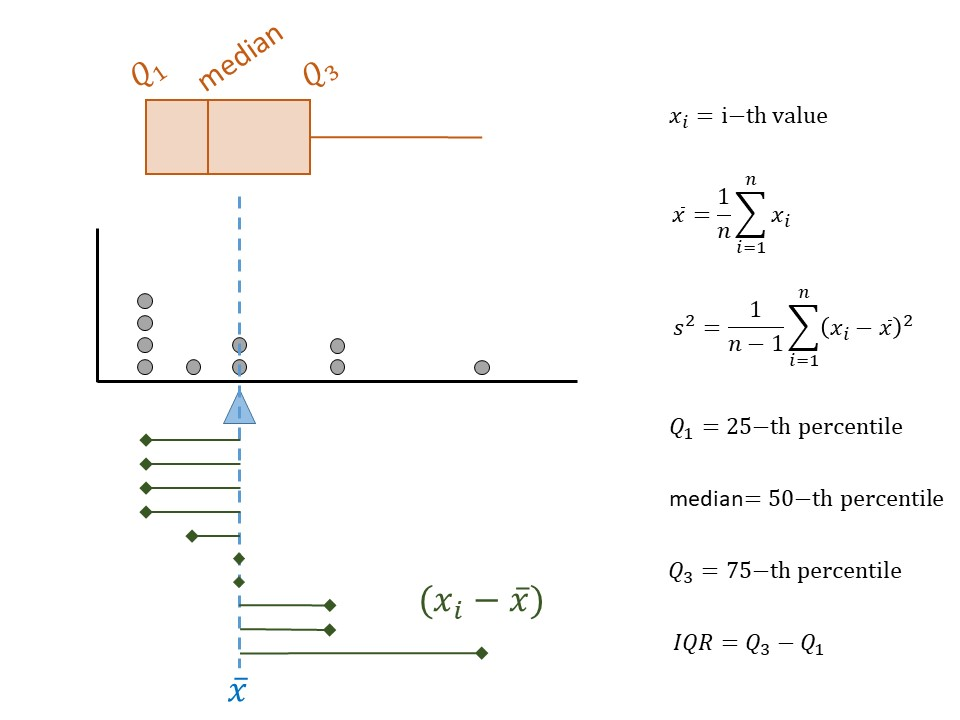
\includegraphics[width=0.8\textwidth,height=\textheight]{./images/Summaries-Summaries.jpg}

}

\caption{\label{fig-summaries-summaries}Illustration of measures of
location and spread for a distribution of values.}

\end{figure}

Finally, consider the \emph{shape} of the distribution of breaking
length we have observed. The breaking length tends to be clustered in
two locations; we call this \emph{bimodal} (each mode is a ``hump'' in
the distribution). Other terms used to describe the shape of a
distribution are \emph{symmetric} and \emph{skewed}. Symmetry refers to
cutting a distribution in half (at the median) and the lower half being
a mirror image of the upper half; skewed distributions are those which
are not symmetric.

Observe that the dot plot above gives us some idea of the location,
spread, and shape of the distribution, in a way that the table of values
could not. This makes it a useful graphic as it is characterizing the
\textbf{distribution of the sample} we have observed. This is one of the
four components of what we call the \emph{Distributional Quartet}.

\begin{definition}[Distribution of the
Sample]\protect\hypertarget{def-distribution-sample}{}\label{def-distribution-sample}

The pattern of variability in the observed values of a variable.

\end{definition}

When the sample is not large, a dot plot is reasonable. Other common
visualizations for a single numeric variable include:

\begin{itemize}
\tightlist
\item
  \emph{jitter plot}: similar to a dot plot, each value observed is
  represented by a dot; the dots are ``jittered'' (shifted randomly) in
  order to avoid over-plotting when many subjects share the same value
  of the response.
\item
  \emph{box plot}: a visual depiction of five key percentiles; the plot
  includes the minimum, first quartile, median, third quartile, and
  maximum value observed. The quartiles are connected with a box, the
  median cuts the box into two components. Occasionally,
  \textbf{outliers} are denoted on the graphic.
\item
  \emph{histogram}: can be thought of as a grouped dot plot in which
  subjects are ``binned'' into groups of similar values. The height of
  each bin represents the number of subjects falling into that bin.
\item
  \emph{density plot}: a smoothed histogram in which the y-axis has been
  standardized so that the area under the curve has value 1. The y-axis
  is not interpretable directly, but higher values along the y-axis
  indicate that the corresponding values on along the x-axis are more
  likely to occur.
\end{itemize}

\begin{definition}[Outlier]\protect\hypertarget{def-outlier}{}\label{def-outlier}

An individual observation which is so extreme, relative to the rest of
the observations in the sample, that it does not appear to conform to
the same distribution.

\end{definition}

To illustrate these graphics, the breaking length for the Paper Strength
example is summarized using various methods in
Figure~\ref{fig-summaries-univariate}. The latter three visualizations
are more helpful when the dataset is very large and plotting the raw
values actually hides the distribution. There is no right or wrong
graphic; it is about choosing the graphic which addresses the question
and adequately portrays the distribution.

\begin{figure}

{\centering 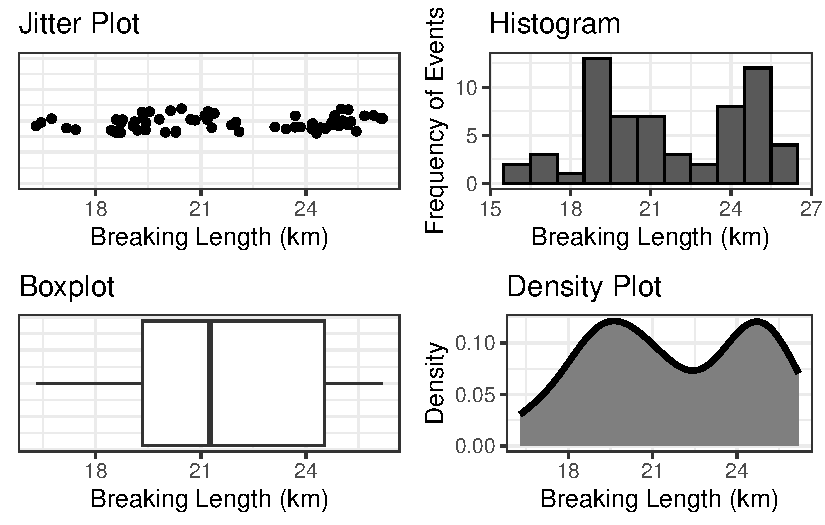
\includegraphics[width=0.8\textwidth,height=\textheight]{./images/fig-summaries-univariate-1.pdf}

}

\caption{\label{fig-summaries-univariate}Four graphical summaries of the
breaking length for the Paper Strength example.}

\end{figure}

The numeric summaries of a distribution are known as
\textbf{statistics}. While parameters characterize a variable at the
population level, statistics characterize a variable at the sample
level.

\begin{definition}[Statistic]\protect\hypertarget{def-statistic}{}\label{def-statistic}

Numeric quantity which summarizes the distribution of a variable within
a \emph{sample}.

\end{definition}

Why would we compute numerical summaries in the sample if we are
interested in the population? Remember the goal of this discipline is to
use the sample to say something about the underlying population. As long
as the sample is representative, the distribution of the sample should
reflect the \textbf{distribution of the population}; therefore,
summaries of the sample should be close to the analogous summaries of
the population (statistics estimate their corresponding parameters). Now
we see the real importance of having a representative sample; it allows
us to say that what we observe in the sample is a good proxy for what is
happening in the population.

\begin{definition}[Distribution of the
Population]\protect\hypertarget{def-distribution-population}{}\label{def-distribution-population}

The pattern of variability in values of a variable at the population
level. Generally, this is impossible to know, but we might model it.

\end{definition}

Statistics being a proxy for the corresponding parameter implies the
mean in the sample should approximate (estimate) the mean in the
population; the standard deviation of the sample should estimate the
standard deviation in the population; and, the shape of the sample
should approximate the shape of the population, etc. The sample is
acting as a representation in all possible ways of the population.

\begin{tcolorbox}[enhanced jigsaw, leftrule=.75mm, coltitle=black, left=2mm, title=\textcolor{quarto-callout-tip-color}{\faLightbulb}\hspace{0.5em}{Big Idea}, breakable, toptitle=1mm, bottomtitle=1mm, colback=white, colbacktitle=quarto-callout-tip-color!10!white, titlerule=0mm, opacitybacktitle=0.6, colframe=quarto-callout-tip-color-frame, bottomrule=.15mm, arc=.35mm, opacityback=0, rightrule=.15mm, toprule=.15mm]

A representative sample reflects the population; therefore, we can use
statistics as estimates of the population parameters.

\end{tcolorbox}

\begin{tcolorbox}[enhanced jigsaw, leftrule=.75mm, coltitle=black, left=2mm, title=\textcolor{quarto-callout-note-color}{\faInfo}\hspace{0.5em}{Note}, breakable, toptitle=1mm, bottomtitle=1mm, colback=white, colbacktitle=quarto-callout-note-color!10!white, titlerule=0mm, opacitybacktitle=0.6, colframe=quarto-callout-note-color-frame, bottomrule=.15mm, arc=.35mm, opacityback=0, rightrule=.15mm, toprule=.15mm]

Notation in any discipline is both important and somewhat arbitrary. We
can choose any symbol we want to represent the sample mean. However, it
is convention that we never use \(\bar{x}\) to represent a parameter
like the mean of the population. The symbol \(\bar{x}\) (or \(\bar{y}\),
etc.) represents observed values being averaged together. Since the
values are observed, we must be talking about the sample, and therefore
\(\bar{x}\) represents a statistic. A similar statement could be made
for \(s^2\) (sample variance) compared to \(\sigma^2\) (population
variance).

Again, in reality, the symbols themselves are not important. The
importance is on their representation. Statistics are observed while
parameters are not.

\end{tcolorbox}

\hypertarget{summarizing-relationships}{%
\section{Summarizing Relationships}\label{summarizing-relationships}}

The summaries discussed above are nice for examining a single variable.
In general, however, research questions of interest typically involve
the relationship between two or more variables. Most graphics are
two-dimensional (though 3-dimensional graphics and even virtual reality
are being utilized now); therefore, summarizing a rich set of
relationships may require the use of both axes as well as color, shape,
size, and even multiple plots in order to tell the right story. We will
explore these various features in upcoming units of the text. Here, we
focus on the need to tell a story that answers the question of interest
instead of getting lost in making a graphic. Consider the following
question from the Deepwater Horizon Case Study described in
\#sec-caseDeepwater:

\begin{quote}
What is the increased risk of developing adverse respiratory symptoms
for volunteers cleaning wildlife compared to those volunteers who do not
have direct exposure to oil?
\end{quote}

Consider the graphic in Figure~\ref{fig-summaries-bad-barchart}; this is
\emph{not} a useful graphic. While it compares the number of volunteers
with symptoms in each group, we cannot adequately address the question
because the research question involves comparing the rates for the two
groups; that is, we are lacking a sense of how many volunteers in each
group did not report symptoms.

\begin{figure}

{\centering 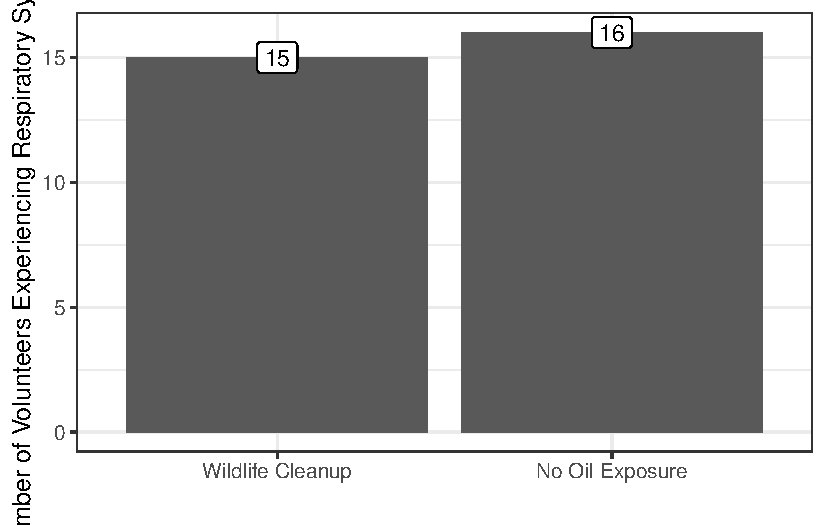
\includegraphics[width=0.8\textwidth,height=\textheight]{./images/fig-summaries-bad-barchart-1.pdf}

}

\caption{\label{fig-summaries-bad-barchart}Illustration of a poor
graphic; the graphic does not give us a sense of the rate within each
group at which volunteers reported symptoms.}

\end{figure}

Instead, Figure~\ref{fig-summaries-good-barchart} compares the rates
within each group. Note that the graphic is still reporting frequency
along the y-axis; that was not the primary problem with
Figure~\ref{fig-summaries-bad-barchart}. However, by reporting
frequencies for both those with respiratory symptoms and those without,
we get a sense of the relative frequency with which respiratory symptoms
occur.

\begin{figure}

{\centering 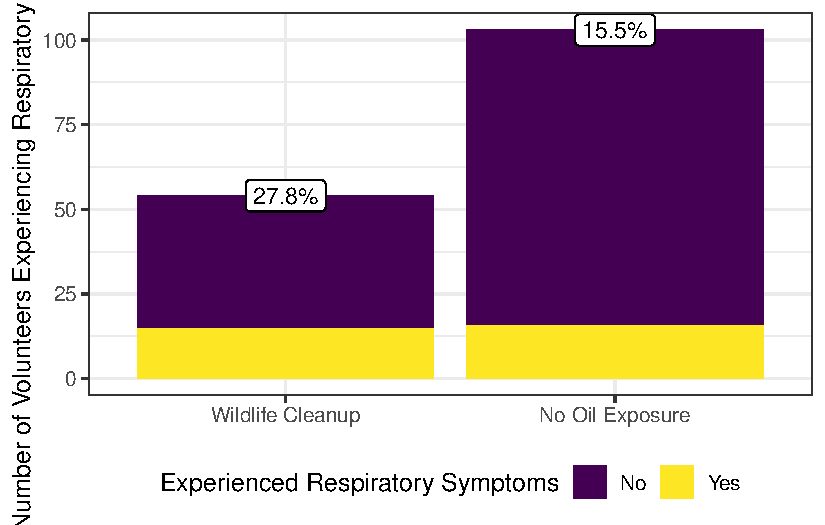
\includegraphics[width=0.8\textwidth,height=\textheight]{./images/fig-summaries-good-barchart-1.pdf}

}

\caption{\label{fig-summaries-good-barchart}Comparison of the rate of
adverse respiratory symptoms among volunteers assigned to different
tasks.}

\end{figure}

From the graphic, it becomes clear that within the sample a higher
fraction of volunteers cleaning wildlife experienced adverse symptoms
compared with those without oil exposure. In fact, volunteers cleaning
wildlife were 1.79 times more likely to experience adverse respiratory
symptoms.

The key to a good summary is understanding the question of interest and
addressing this question through a useful characterization of the
variability.

\part{Unit III: Fundamentals of Bayesian Inference}

Once we have data, we want to use it to say something about the
underlying population. This is the process of ``drawing inference.''
There are two large paradigms in the statistical community for defining
the framework under which inference occurs. This unit introduces the
fundamental components of the Bayesian paradigm. We focus on the
mechanics in scenarios for which the process is analytically tractable
by hand. The remainder of the text merely illustrates these principles
in more complex scenarios.

\hypertarget{sec-bayesrule}{%
\chapter{Bayes Rule}\label{sec-bayesrule}}

\providecommand{\norm}[1]{\lVert#1\rVert}
\providecommand{\abs}[1]{\lvert#1\rvert}
\providecommand{\iid}{\stackrel{\text{IID}}{\sim}}
\providecommand{\ind}{\stackrel{\text{Ind}}{\sim}}

\providecommand{\bm}[1]{\mathbf{#1}}
\providecommand{\bs}[1]{\boldsymbol{#1}}
\providecommand{\bbeta}{\bs{\beta}}

\providecommand{\Ell}{\mathcal{L}}
\providecommand{\indep}{\perp\negthickspace\negmedspace\perp}

In a probability course, Bayes' Rule is often presented as a neat trick
for solving a particular type of problem involving two events. While
this simple class of problems understates its true potential, it does
serve as a way of highlighting the key idea behind the method.

\begin{example}[Disease
Testing]\protect\hypertarget{exm-disease}{}\label{exm-disease}

An enzyme-linked immunosorbent assay (ELISA) test is performed to
determine if the human immunodeficiency virus (HIV) is present in the
blood of individuals. Suppose that the ELISA test correctly indicates
HIV 99\% of the time, and it correctly indicates being HIV-free in
99.5\% of cases. Finally, suppose that the prevalence of HIV among blood
donors is known to be 1/10000. What is the probability an individual who
testes positive is actually infected with HIV?

\end{example}

In this example, we are interested in the probability of an individual
being infected with HIV \emph{given} their test is positive. Recalling
the definition of conditional probability
(Theorem~\ref{thm-conditional-probability}), we consider

\[Pr(\text{Infected with HIV} \mid \text{Tests Positive}) = \frac{Pr(\text{Infected with HIV} \cap \text{Tests Positive})}{Pr(\text{Tests Positive})};\]

however, these probabilities are not provided in the problem. What we
actually have are the probability of testing positive given the patient
is infected with HIV (0.99), the probability of testing negative given
the patient is not infected with HIV (0.95), and the probability of
having HIV (1/10000). This is the power of Bayes' Rule --- it allows you
to address problems by reversing the conditioning. That is, we can make
a statement about the likelihood of \(A\) given \(B\) using information
about the likelihood of \(B\) given \(A\)! As we state Bayes Rule, we
keep in mind that it is not the rule itself which is innovative but (a)
what the rule implies and (b) how we apply it to solve problems in
statistical inference, that make it valuable.

\begin{theorem}[Bayes Theorem for Two
Events]\protect\hypertarget{thm-simple-bayes-rule}{}\label{thm-simple-bayes-rule}

Given events \(A\) and \(B\) such that \(Pr(A), Pr(B) \neq 0\), then we
have that

\[Pr(A \mid B) = \frac{Pr(B \mid A)Pr(A)}{Pr(B \mid A)Pr(A) + Pr(B \mid A^\mathsf{c}) Pr(A^\mathsf{c})}\]

\end{theorem}

Bayes' Rule is actually a convenient wrapper for an application of
several other basic probability results combined:

\begin{itemize}
\tightlist
\item
  The numerator is an application of the definition of conditional
  probability; we can always write a joint probability (``and
  statement'') as the product of a conditional probability and a
  marginal probability.
\item
  The denominator is the result of the total probability rule; a
  marginal probability is computed by summing over mutually exclusive
  joint probabilities, which again are rewritten similarly to the
  numerator.
\end{itemize}

\begin{tcolorbox}[enhanced jigsaw, leftrule=.75mm, coltitle=black, left=2mm, title=\textcolor{quarto-callout-tip-color}{\faLightbulb}\hspace{0.5em}{Big Idea}, breakable, toptitle=1mm, bottomtitle=1mm, colback=white, colbacktitle=quarto-callout-tip-color!10!white, titlerule=0mm, opacitybacktitle=0.6, colframe=quarto-callout-tip-color-frame, bottomrule=.15mm, arc=.35mm, opacityback=0, rightrule=.15mm, toprule=.15mm]

Bayes' Rule says that our information about \(A\), \emph{after}
observing \(B\), can be stated in terms of what we know about \(B\)
after observing \(A\) and our belief about \(A\) \emph{prior} to seeing
\(B\).

\end{tcolorbox}

The above is useful when talking about two events, but the majority of
applications address random variables, not specific events. That is, we
are interested in characterizing entire distributions, not just
probabilities for specific events. Following the same logic as above, we
are able to extend (from a total probability rule and from the
definition of conditional probability) the above result to two random
variables.

\begin{theorem}[Bayes Theorem for Two Random
Variables]\protect\hypertarget{thm-rv-bayes-rule}{}\label{thm-rv-bayes-rule}

Let \(X\) and \(Y\) be two random variables; then, we have that

\[f_{Y \mid X}(y \mid x) = \frac{f_{X \mid Y}(x \mid y) f_Y(y)}{\int_{\mathcal{S}_Y} f_{X \mid Y}(x \mid y) f_Y(y) dy},\]

where the integration is replaced by summation when necessary to account
for a discrete random variable.

\end{theorem}

\begin{tcolorbox}[enhanced jigsaw, leftrule=.75mm, coltitle=black, left=2mm, title=\textcolor{quarto-callout-note-color}{\faInfo}\hspace{0.5em}{Note}, breakable, toptitle=1mm, bottomtitle=1mm, colback=white, colbacktitle=quarto-callout-note-color!10!white, titlerule=0mm, opacitybacktitle=0.6, colframe=quarto-callout-note-color-frame, bottomrule=.15mm, arc=.35mm, opacityback=0, rightrule=.15mm, toprule=.15mm]

We will not distinguish between continuous and discrete random
variables. For compactness, all results are presented assuming
continuous random variables. When necessary, replace integration with
summation (as summation is really just integration with respect to a
specific measure).

\end{tcolorbox}

As stated above, this result is really the application of basic
definitions covered in a probability course. But, they are worth
revisiting.

\begin{definition}[Conditional
Density]\protect\hypertarget{def-conditional-density}{}\label{def-conditional-density}

Let \(X\) and \(Y\) be two random variables; the conditional density of
\(X\) given \(Y\) is

\[f_{X \mid Y}(y \mid x) = \frac{f_{X, Y}(x, y)}{f_Y(y)}\]

\end{definition}

\begin{tcolorbox}[enhanced jigsaw, leftrule=.75mm, coltitle=black, left=2mm, title=\textcolor{quarto-callout-note-color}{\faInfo}\hspace{0.5em}{Note}, breakable, toptitle=1mm, bottomtitle=1mm, colback=white, colbacktitle=quarto-callout-note-color!10!white, titlerule=0mm, opacitybacktitle=0.6, colframe=quarto-callout-note-color-frame, bottomrule=.15mm, arc=.35mm, opacityback=0, rightrule=.15mm, toprule=.15mm]

Subscripts are to denote which random variable is being discussed; so,
\(f_X(x)\) refers to the density function of the random variable \(X\)
evaluated at \(x\). We suppress the subscripts when the context makes it
clear which random variable is being referenced.

\end{tcolorbox}

Rearranging the terms in Definition~\ref{def-conditional-density}, we
are able to see that any joint density function \(f_{X, Y}(x, y)\) can
be written as the product of a conditional density and a marginal
density. Similarly, we can write any marginal density by integrating
over a joint density.

\begin{theorem}[Total Probability Rule for Random
Variables]\protect\hypertarget{thm-total-probability-rule}{}\label{thm-total-probability-rule}

Let \(X\) and \(Y\) be two random variables with joint density
\(f_{X,Y}(x,y)\); then, the marginal density of \(X\) is given by

\[f_X(x) = \int_{\mathcal{S}_Y} f_{X,Y}(x, y) dy,\]

where \(\mathcal{S}_Y\) is the support of \(Y\).

\end{theorem}

To add a little more intuition to this result, let \(X\) represent the
grade in this course, and suppose we are interested in the event that
\(X\) takes the value ``A.'' Well, this course is most certainly
impacted by your other courses; so, let \(Y\) take the value of the
grade in the hardest class remaining on your schedule. Then, there are
only a certain number of options:

\begin{itemize}
\tightlist
\item
  \(X\) takes the value ``A'' while \(Y\) takes the value ``A'' (whoo
  hoo!);
\item
  \(X\) takes the value ``A'' while \(Y\) takes the value ``B'';
\item
  \(X\) takes the value ``A'' while \(Y\) takes the value ``C'';
\item
  \(X\) takes the value ``A'' while \(Y\) takes the value ``D''; and,
\item
  \(X\) takes the value ``A'' while \(Y\) takes the value ``F'' (let's
  hope not).
\end{itemize}

Each of these has some probability of occurring. Since this exhausts all
possibilities for \(Y\), then we can determine the probability of \(X\)
by summing the probability of each of these mutually exclusive events.
The above lemma captures that we can do this for all values in the
support of \(X\) simultaneously. Essentially, we have a partition across
the support of \(X\) based on the value of \(Y\); then, we compute the
probability of \(X\) by summing over the partition.

The above definition is sufficient for several applications. However, it
is worth stating the theorem from the most general of perspectives. To
do so, we need to define the concept of a random vector.

\begin{definition}[Random
Vector]\protect\hypertarget{def-random-vector}{}\label{def-random-vector}

Let \(X_1, X_2, \dots, X_n\) be \(n\) random variables. Then, the vector
\(\mathbf{X} = \left(X_1, X_2, \dots, X_n\right)^\top\) is a random
vector of length \(n\).

\end{definition}

A random vector is essentially a vector comprised of random components.
This will be necessary moving forward because we typically have samples
of size \(n > 1\).

\begin{theorem}[Bayes
Theorem]\protect\hypertarget{thm-bayes-rule}{}\label{thm-bayes-rule}

Let \(\mathbf{X}\) and \(\mathbf{Y}\) be two random \emph{vectors}.
Then, we have that

\[f_{\mathbf{Y} \mid \mathbf{X}}(\mathbf{y} \mid \mathbf{x}) = \frac{f_{\mathbf{X} \mid \mathbf{Y}}(\mathbf{x} \mid \mathbf{y}) f_{\mathbf{Y}}(\mathbf{y})}{\int_{\mathcal{S}_\mathbf{Y}} f_{\mathbf{X} \mid \mathbf{Y}}(\mathbf{x} \mid \mathbf{y}) f_{\mathbf{Y}}(\mathbf{y}) d\mathbf{y}}\]

where the integral is now a multi-dimensional integral. Integration for
any component is replaced by summation when needed.

\end{theorem}

\hypertarget{tenants-of-the-bayesian-approach-to-inference}{%
\section{Tenants of the Bayesian Approach to
Inference}\label{tenants-of-the-bayesian-approach-to-inference}}

The above results on their own may be interesting in a probability
course. However, we are interested primarily in their application when
we have observed a sample from a population which is not fully known.
Before we delve into the mechanics, let's pause to reflect on how we
intend to apply these results.

Recall that statistics is about using a sample to make inference on the
population. Specifically, we will posit a model for the distribution of
a response within the population; however, that model will be specified
only up to some unknown parameters. There are two general statistical
paradigms for performing inference, and these stem from two different
questions we might ask:

\begin{itemize}
\tightlist
\item
  Given a hypothesis about the parameters is true, how likely is the
  observed data?
\item
  Given the observed data, how likely is a particular hypothesis about
  the parameters?
\end{itemize}

The first question results in the classical Frequentist perspective
(most statistical courses) and a frequentist interpretation of
probability. The second results in the Bayesian perspective and a
subjective interpretation of probability.

Prior to collecting data, we might have some belief about the the
unknown parameters that govern our model for the population. Then, we
collect a sample from the population; since this data is representative
of the population, it must contain information about those parameters.
Therefore, we want to update our belief about the parameters in light of
this data. That is the Bayesian process in a nutshell.

\begin{tcolorbox}[enhanced jigsaw, leftrule=.75mm, coltitle=black, left=2mm, title=\textcolor{quarto-callout-important-color}{\faExclamation}\hspace{0.5em}{Tenants of the Bayesian Approach to Inference}, breakable, toptitle=1mm, bottomtitle=1mm, colback=white, colbacktitle=quarto-callout-important-color!10!white, titlerule=0mm, opacitybacktitle=0.6, colframe=quarto-callout-important-color-frame, bottomrule=.15mm, arc=.35mm, opacityback=0, rightrule=.15mm, toprule=.15mm]

Every analysis in this course is built on the following three tenants:

\begin{enumerate}
\def\labelenumi{\arabic{enumi}.}
\tightlist
\item
  The Bayesian approach takes into account \emph{prior} knowledge when
  making inference.
\item
  The Bayesian approach uses probability models to \emph{quantify
  uncertainty} in the parameters.
\item
  The Bayesian approach \emph{updates} our prior knowledge conditional
  on the observed data.
\end{enumerate}

\end{tcolorbox}

Throughout, we will rely on a subjective view of probability. That is,
probability characterizes how sure you are of something. So, it does not
make sense to say ``how likely is it to rain tomorrow?'' There is no one
probability that answers this question. Instead, we will always have
(even if not explicitly stated) a ``how likely \emph{do you
believe}\ldots'\,' element to our question. That is, we are always
bringing in our personal (subjective) opinion. This can be very
uncomfortable for some of us --- the idea of there not being a
single''right'' answer. We will save this discussion for a future
chapter.

\hypertarget{sec-modelingsamples}{%
\chapter{Modeling Samples}\label{sec-modelingsamples}}

\providecommand{\norm}[1]{\lVert#1\rVert}
\providecommand{\abs}[1]{\lvert#1\rvert}
\providecommand{\iid}{\stackrel{\text{IID}}{\sim}}
\providecommand{\ind}{\stackrel{\text{Ind}}{\sim}}

\providecommand{\bm}[1]{\mathbf{#1}}
\providecommand{\bs}[1]{\boldsymbol{#1}}
\providecommand{\bbeta}{\bs{\beta}}

\providecommand{\Ell}{\mathcal{L}}
\providecommand{\indep}{\perp\negthickspace\negmedspace\perp}

Rarely is our data a single observation. Instead, we collect a sample of
observations. As a result, we must be able to comfortably model a
\emph{collection} of random variables.

In a probability course, we are generally concerned with modeling a
single random variable. The course may build into modeling the joint
distribution of two random variables, but generally not further.
However, if each random variable represents a single measurement taken
on a unit observation, then taking measurements on a sample of \(n\)
observations is actually a collection of \(n\) random variables. Part of
quantifying our uncertainty in a parameter is first modeling the process
that generated the data as a function of that parameter; that means, we
need to model the distribution of the responses.

\begin{tcolorbox}[enhanced jigsaw, leftrule=.75mm, coltitle=black, left=2mm, title=\textcolor{quarto-callout-note-color}{\faInfo}\hspace{0.5em}{Note}, breakable, toptitle=1mm, bottomtitle=1mm, colback=white, colbacktitle=quarto-callout-note-color!10!white, titlerule=0mm, opacitybacktitle=0.6, colframe=quarto-callout-note-color-frame, bottomrule=.15mm, arc=.35mm, opacityback=0, rightrule=.15mm, toprule=.15mm]

We often talk about ``modeling the data,'' but that is not precise
language. The \emph{data} is fixed; it is not modeled. We are modeling
the \emph{process} which generated that data --- it is this process that
produces random values which are then observed.

\end{tcolorbox}

Let \(X_1, X_2, \dotsc, X_n\) represent \(n\) observations of the same
variable we intend to make (note the future tense). We group these in a
random vector \(\mathbf{X}\) of length \(n\). Not only are we interested
in how each \emph{element} in \(\mathbf{X}\) is distributed, we are also
interested in modeling how they are interrelated.

\begin{definition}[Joint
Density]\protect\hypertarget{def-joint-density}{}\label{def-joint-density}

For a random vector \(\mathbf{X}\), the function
\(f_{\mathbf{X}}(\mathbf{x})\) such that for any set
\(A \in \mathbb{R}^n\), we have

\[Pr(\mathbf{X} \in A) = \int \dotsi \int_{A} f_{\mathbf{X}}(\mathbf{x}) dx_1 \dotsb dx_n\]

is called the joint density function; this is also referred to as the
\emph{likelihood}. Integrals are replaced by sums when appropriate.

\end{definition}

\begin{tcolorbox}[enhanced jigsaw, leftrule=.75mm, coltitle=black, left=2mm, title=\textcolor{quarto-callout-tip-color}{\faLightbulb}\hspace{0.5em}{Big Idea}, breakable, toptitle=1mm, bottomtitle=1mm, colback=white, colbacktitle=quarto-callout-tip-color!10!white, titlerule=0mm, opacitybacktitle=0.6, colframe=quarto-callout-tip-color-frame, bottomrule=.15mm, arc=.35mm, opacityback=0, rightrule=.15mm, toprule=.15mm]

Probabilities involving multiple random variables involve integration
over the joint density.

\end{tcolorbox}

The joint density describes how the elements move together; if we are
interested in only a single element, we consider the marginal density,
which is accomplished by integrating (or summing) over all possible
values for the \emph{other} elements.

\begin{definition}[Marginal
Density]\protect\hypertarget{def-marginal-density}{}\label{def-marginal-density}

For a random vector \(\mathbf{X}\), the marginal density of the first
component \(X_1\) (without loss of generality) is

\[f_{X_1}(u) = \int \dotsi \int f_{\mathbf{X}}(\mathbf{x}) dx_2 \dotsb dx_n.\]

\end{definition}

Bayes Theorem, and therefore Bayesian data analysis, is primarily
concerned with conditional densities, which also generalize to random
vectors.

\begin{definition}[Conditional
Density]\protect\hypertarget{def-conditional-density}{}\label{def-conditional-density}

Let \(\mathbf{X}\) be a random vector; without loss of generality,
partition \(\mathbf{X}\) such that

\[\mathbf{X} = \begin{pmatrix} \mathbf{X}_1 \\ \mathbf{X}_2 \end{pmatrix}\]

where \(\mathbf{X}_1\) represents the first \(k\) components and
\(\mathbf{X}_2\) represents the remaining \(n-k\) components. Then, the
conditional density of \(\mathbf{X}_1\) given \(\mathbf{X}_2\) is

\[f_{\mathbf{X}_1 \mid \mathbf{X}_2}(\mathbf{x}_1 \mid \mathbf{x}_2) = \frac{f_{\mathbf{X}}(\mathbf{x})}{f_{\mathbf{X}_2}(\mathbf{x}_2)}.\]

\end{definition}

It is worth noting that with respect to the components of interest
\(\mathbf{X}_1\), the denominator in the conditional density is just a
constant scaling factor to ensure the density integrates/sums to 1; that
is, \emph{with respect to the variables of interest}, the denominator is
a constant.

\begin{tcolorbox}[enhanced jigsaw, leftrule=.75mm, coltitle=black, left=2mm, title=\textcolor{quarto-callout-note-color}{\faInfo}\hspace{0.5em}{Note}, breakable, toptitle=1mm, bottomtitle=1mm, colback=white, colbacktitle=quarto-callout-note-color!10!white, titlerule=0mm, opacitybacktitle=0.6, colframe=quarto-callout-note-color-frame, bottomrule=.15mm, arc=.35mm, opacityback=0, rightrule=.15mm, toprule=.15mm]

When we are working with named distributions, using statistical software
to compute probabilities is often superior to generic calculus software.
This is because the algorithms for computing these probabilities are
more stable for known distributions than general all-purpose numerical
integration methods.

\end{tcolorbox}

\hypertarget{independent-and-identically-distributed}{%
\section{Independent and Identically
Distributed}\label{independent-and-identically-distributed}}

The above discussion, while accurate, is unrealistic in that it begins
with a completely formed likelihood. In reality, we must posit models
which correspond to the data generating process. Positing a model for
the distribution of an individual observation (element of
\(\mathbf{X}\)) often means choosing from among well-known named
probability models. Regardless of whether a named model is used or a
custom model constructed, the process always involves examining the
context to determine an appropriate structure --- the shape and support
--- of the distribution. We then allow the parameters of this
distribution to remain unknown. This is where we turn from probability
to statistics --- suddenly, our models are only partly known, and there
are some aspects (the parameters governing the behavior of the model)
which are unknown. We will use data to make some statements about these
parameters to address questions of interest which are framed in terms of
these parameters.

Instead of trying to model the joint distribution of the observed data
directly, we often model the variability in the individual observations.
We then place additional conditions on the relationship between the
observations in order to develop the joint distribution. One of the most
popular conditions is that of independence.

\begin{definition}[Independence]\protect\hypertarget{def-independence}{}\label{def-independence}

Random variables \(X_1, X_2, \dotsc, X_n\) are said to be mutually
independent (or just ``independent'') if and only if

\[Pr\left(X_1 \in A_1, X_2 \in A_2, \dotsb, X_n \in A_n\right) = \prod_{i=1}^{n} Pr\left(X_i \in A_i\right),\]

where \(A_1, A_2, \dotsc, A_n\) are arbitrary sets. Perhaps more
helpful, \(X_1, X_2, \dotsc, X_n\) are said to be mutually independent
if and only if

\[f_{\mathbf{X}}(\mathbf{x}) = \prod_{i=1}^{n} f_{X_i}\left(x_i\right).\]

\end{definition}

\begin{tcolorbox}[enhanced jigsaw, leftrule=.75mm, coltitle=black, left=2mm, title=\textcolor{quarto-callout-note-color}{\faInfo}\hspace{0.5em}{Note}, breakable, toptitle=1mm, bottomtitle=1mm, colback=white, colbacktitle=quarto-callout-note-color!10!white, titlerule=0mm, opacitybacktitle=0.6, colframe=quarto-callout-note-color-frame, bottomrule=.15mm, arc=.35mm, opacityback=0, rightrule=.15mm, toprule=.15mm]

For those not familiar, \(\prod_{i=1}^n a_i\) is the \emph{product
operator}. It is analogous to \(\sum_{i=1}^{n} a_i\), but uses products
instead of sums.

\end{tcolorbox}

Essentially, a random variable \(X\) is said to be independent of \(Y\)
if the likelihood that \(X\) takes a particular value is the same
regardless of the value \(Y\) takes.

Assuming independence allows us to easily construct joint densities by
taking the product of the marginal density for each observation.
Independence is a powerful condition when constructing likelihoods.
However, it cannot be blindly enforced; we should take caution when
assuming independence. This requires considering the method in which the
data was obtained to determine if it is reasonable that the value of one
observation does not affect the likelihood of any other observation.

Ideally, when we take a sample, each observation is representative of
the same process. This is what allows us to use all observations in a
sample in order to make inference --- we believe that each observation
is able to contribute information about the unknown parameter. Believing
that each observation is representative of the same process is
essentially assume that each corresponding random variable (prior to
observing the data) has the same distribution.

\begin{definition}[Identically
Distributed]\protect\hypertarget{def-identically-distributed}{}\label{def-identically-distributed}

We say that random variables \(X\) and \(Y\) are identically distributed
if \(F_X(u) = F_Y(u)\) for all \(u\). This is equivalent to saying the
two random variables have the same density function \(f\).

\end{definition}

\begin{tcolorbox}[enhanced jigsaw, leftrule=.75mm, coltitle=black, left=2mm, title=\textcolor{quarto-callout-warning-color}{\faExclamationTriangle}\hspace{0.5em}{Warning}, breakable, toptitle=1mm, bottomtitle=1mm, colback=white, colbacktitle=quarto-callout-warning-color!10!white, titlerule=0mm, opacitybacktitle=0.6, colframe=quarto-callout-warning-color-frame, bottomrule=.15mm, arc=.35mm, opacityback=0, rightrule=.15mm, toprule=.15mm]

Let \(X\) and \(Y\) be identically distributed random variables. This
does not mean that \(X = Y\). ``Identically distributed'' says the two
random variables have the same distribution, not the same value. As a
result, they share the same mean, variance, etc.

\end{tcolorbox}

When the observations in our sample are both independent and identically
distributed, we say we have a ``random sample.''

\begin{definition}[Random
Sample]\protect\hypertarget{def-random-sample}{}\label{def-random-sample}

A random sample of size \(n\) refers to a collection of \(n\) random
variables \(X_1, X_2, \dotsc, X_n\) such that the random variables are
mutually independent, and the distribution of each random variable is
identical.

\end{definition}

\begin{example}[Delivery by Cesarean Section
(C-section)]\protect\hypertarget{exm-csec}{}\label{exm-csec}

It is sometimes necessary for babies to be delivered through a surgical
procedure known as a Cesarean Section (C-section). As surgical
procedures carry risk, a C-section is typically performed when a vaginal
delivery would place the infant or mother in undue risk of
complications. Suppose we are interested in characterizing the hospital
experiences of mothers who have undergone a C-section at Union Hospital
in Terre Haute, Indiana.

For this community health project, we would like to survey \(n = 15\)
mothers who have undergone a C-section. Of course, not every delivery is
a C-section; let \(X_i\) represent the number of vaginal deliveries that
occur \emph{between} the \(i\)-th C-section and the previous C-section
we observe.

Suppose we are willing to believe that (absent any additional
information on the pregnancy) each patient in the labor and delivery
ward has the same probability of undergoing a C-section; further,
whether one patient undergoes a C-section is independent of any other
patient undergoing a C-section. Develop a model for the likelihood of
the data to be observed.

\end{example}

\begin{solution}

We begin by thinking about the specific context. Note, for example, that
\(X_i\) is a non-negative integer; that is,
\(X_i \in \{0, 1, 2, \dotsc \}\). Let \(\theta\) represent the
probability that a patient undergoes a C-section (and therefore
\(1 - \theta\) represents the probability of a vaginal birth). Since we
believe the method of delivery for one patient is independent of the
method of delivery for all other patients, and that each probability of
a delivery by C-section is the same for each patient, then it is
reasonable to state that

\[Pr\left(X_i = x\right) = \theta (1 - \theta)^x \qquad x = 0, 1, 2, \dotsc.\]

That is, \(X_i\) follows a Geometric distribution with parameter
\(\theta\). This distribution captures the idea that \(x\) vaginal
deliveries occur (each with probability \(1 - \theta\)) before we see
the \(i\)-th C-section (which occurs with probability \(\theta\)).

Further, since each birth is independent, we can consider
\(X_1, X_2, \dotsc, X_n\) to be a random sample. Letting
\(\mathbf{X} = \left(X_1, X_2, \dotsc, X_n\right)^\top\) be the random
vector of observations, the likelihood is given by

\begin{equation}\protect\hypertarget{eq-csec-likelihood}{}{
\begin{aligned}
  f(\mathbf{x} \mid \theta)
    &= \prod_{i=1}^{n} f_{X_i}\left(x_i \mid \theta\right) \\
    &= \prod_{i=1}^{n} \theta (1 - \theta)^{x_i} \\
    &= \theta^n (1 - \theta)^{\sum_{i=1}^{n} x_i} \\
    &= \theta^n (1 - \theta)^{n\bar{x}}.
\end{aligned}
}\label{eq-csec-likelihood}\end{equation}

Note that line (1) makes use of the independence to say the likelihood
is the product of the marginal density functions of each observation.
Line (2) makes use of that each observation is identically distributed;
this means that each observation has the same functional family for the
density and is governed by the same parameter. This still allows \(x_i\)
to differ from \(x_j\), but the distribution is the same. Line (3)
brings the product through the expression, with the product of
exponentials with the same base resulting in adding the exponents. Line
(4) simplifies the expression; for notational simplicity, we prefer
\(n\bar{x}\) to \(\sum_{i=1}^{n} x_i\), though the two are equivalent.

We also note that the likelihood expressly acknowledges the dependence
on the parameter \(\theta\) by using \(f(\mathbf{x} \mid \theta)\)
instead of just \(f(\mathbf{x})\).

\end{solution}

\begin{tcolorbox}[enhanced jigsaw, leftrule=.75mm, coltitle=black, left=2mm, title=\textcolor{quarto-callout-note-color}{\faInfo}\hspace{0.5em}{Note}, breakable, toptitle=1mm, bottomtitle=1mm, colback=white, colbacktitle=quarto-callout-note-color!10!white, titlerule=0mm, opacitybacktitle=0.6, colframe=quarto-callout-note-color-frame, bottomrule=.15mm, arc=.35mm, opacityback=0, rightrule=.15mm, toprule=.15mm]

It is helpful to be in the habit acknowledging the dependence of the
likelihood on the parameter.

\end{tcolorbox}

\begin{tcolorbox}[enhanced jigsaw, leftrule=.75mm, coltitle=black, left=2mm, title=\textcolor{quarto-callout-tip-color}{\faLightbulb}\hspace{0.5em}{Big Idea}, breakable, toptitle=1mm, bottomtitle=1mm, colback=white, colbacktitle=quarto-callout-tip-color!10!white, titlerule=0mm, opacitybacktitle=0.6, colframe=quarto-callout-tip-color-frame, bottomrule=.15mm, arc=.35mm, opacityback=0, rightrule=.15mm, toprule=.15mm]

By placing conditions on how the data is generated, we are able to model
the joint distribution of the responses. This is sometimes referred to
as the \emph{likelihood} of the unknown parameters; we also refer to it
as the model for the data generating process, as it explains the
variability in the observed data.

\end{tcolorbox}

\hypertarget{sec-priors}{%
\chapter{Quantifying/Modeling Prior Information}\label{sec-priors}}

\providecommand{\norm}[1]{\lVert#1\rVert}
\providecommand{\abs}[1]{\lvert#1\rvert}
\providecommand{\iid}{\stackrel{\text{IID}}{\sim}}
\providecommand{\ind}{\stackrel{\text{Ind}}{\sim}}

\providecommand{\bm}[1]{\mathbf{#1}}
\providecommand{\bs}[1]{\boldsymbol{#1}}
\providecommand{\bbeta}{\bs{\beta}}

\providecommand{\Ell}{\mathcal{L}}
\providecommand{\indep}{\perp\negthickspace\negmedspace\perp}

Data contributes information to, and therefore impacts, our beliefs.
But, prior to beginning a study, we generally have some established
beliefs --- based on previous studies, expert opinions, personal
experience, etc. The Bayesian framework explicitly incorporates these
established \emph{prior} beliefs in the analysis. The beliefs just need
to be quantified.

\begin{tcolorbox}[enhanced jigsaw, leftrule=.75mm, coltitle=black, left=2mm, title=\textcolor{quarto-callout-tip-color}{\faLightbulb}\hspace{0.5em}{Big Idea}, breakable, toptitle=1mm, bottomtitle=1mm, colback=white, colbacktitle=quarto-callout-tip-color!10!white, titlerule=0mm, opacitybacktitle=0.6, colframe=quarto-callout-tip-color-frame, bottomrule=.15mm, arc=.35mm, opacityback=0, rightrule=.15mm, toprule=.15mm]

The Bayesian framework encodes any uncertainty through probability
distributions.

\end{tcolorbox}

Before we examine the technical aspects of quantifying the beliefs we
have prior to the start of a study, we need to consider how this fits
into the larger scope of performing inference. Recall that our primary
aim is to make some statement about the population using a corresponding
sample. Further, we have some model for the data generating process up
to some unknown parameters (this was the focus of the previous chapter).
When we collect data, it provides additional information about these
unknown parameters. That is, the data impacts the beliefs we have about
these unknown parameters. Similarly, any beliefs we have entering the
study must relate to these unknown parameters.

Prior to beginning the study, we generally have some notion about the
parameters that govern the data generating process. What is a typical
GPA for a college student? How much does a member of the mathematics
faculty earn each year, on average? While we use data to inform these
beliefs (topic of the next chapter), even without data available, we
have some idea of where we think the answer lies. Bayesians encode these
beliefs into probability distributions. The beliefs we have prior to
seeing the data are described by a ``prior'' distribution, since the
beliefs were those we had \emph{a priori}.

\begin{definition}[Prior
Distribution]\protect\hypertarget{def-prior-distribution}{}\label{def-prior-distribution}

A distribution quantifying our beliefs about uncertainty in the
\emph{parameter(s)} of the underlying sampling distribution \emph{prior
to} observing any data. This is often denoted by
\(\pi(\boldsymbol{\theta})\) where \(\boldsymbol{\theta}\) is the
parameter vector.

\begin{itemize}
\tightlist
\item
  This relies on a \emph{subjective} view of probability.
\item
  As prior beliefs are subjective, there is no ``one'' prior, but each
  individual may have a unique prior.
\end{itemize}

\end{definition}

Constructing a prior distribution is not all that different from
constructing the likelihood. There are several aspects involved, but it
is all about understanding the structure of the beliefs.

\begin{tcolorbox}[enhanced jigsaw, leftrule=.75mm, coltitle=black, left=2mm, title=\textcolor{quarto-callout-note-color}{\faInfo}\hspace{0.5em}{Tips for Constructing a Prior}, breakable, toptitle=1mm, bottomtitle=1mm, colback=white, colbacktitle=quarto-callout-note-color!10!white, titlerule=0mm, opacitybacktitle=0.6, colframe=quarto-callout-note-color-frame, bottomrule=.15mm, arc=.35mm, opacityback=0, rightrule=.15mm, toprule=.15mm]

The following considerations should be kept in mind when constructing
the prior distribution.

\begin{itemize}
\tightlist
\item
  Identify the unknown parameter(s). That is, on what unknown value(s)
  does the \emph{likelihood} (model for the data generating process)
  depend?
\item
  Describe the support for the parameter(s).
\item
  Use clear statements about our beliefs of the parameters to determine
  the \textbf{hyperparameters}.
\end{itemize}

\end{tcolorbox}

\begin{definition}[Hyperparameter]\protect\hypertarget{def-hyperparameter}{}\label{def-hyperparameter}

A constant term of a prior distribution that characterizes the family we
are considering.

\end{definition}

\begin{tcolorbox}[enhanced jigsaw, leftrule=.75mm, coltitle=black, left=2mm, title=\textcolor{quarto-callout-note-color}{\faInfo}\hspace{0.5em}{Note}, breakable, toptitle=1mm, bottomtitle=1mm, colback=white, colbacktitle=quarto-callout-note-color!10!white, titlerule=0mm, opacitybacktitle=0.6, colframe=quarto-callout-note-color-frame, bottomrule=.15mm, arc=.35mm, opacityback=0, rightrule=.15mm, toprule=.15mm]

It is sometimes said that a hyperparameter is a ``parameter'' of the
prior distribution. You want to distinguish between ``parameters''
(constant terms that characterize the likelihood), which are unknown,
and hyperparameters (constant terms that characterize a prior), which
are known values chosen such that the prior distribution reflects our
prior beliefs.

\end{tcolorbox}

\begin{example}[A Naive Classification of College
Students]\protect\hypertarget{exm-naive}{}\label{exm-naive}

Rose-Hulman Institute of Technology (RHIT) and Indiana State University
(ISU) are located in Terre Haute, IN. While both colleges cater to
undergraduate students, they have different profiles. For the 2021-2022
academic year,
\href{https://irt2.indstate.edu/cms7/ir/assets/File/CDS22.pdf}{Indiana
State University reported} having 5738 full-time undergraduate students,
3232 (56.3\%) of which identified as female. For the same year,
\href{https://www.rose-hulman.edu/academics/academic-affairs/irpa/reports/CDS_AY_2021-22.pdf}{Rose-Hulman
reported} having 2058 full-time undergraduate students, 507 (24.6\%) of
which identified as female.

Suppose an individual sees a group of 10 college students hanging out at
a coffee shop in Terre Haute; they are interested in determining which
college the students attend. If the students attend ISU, then we would
expect 56.3\% to identify as female; if the students attend RHIT, then
we would expect 24.6\% to identify as female. However, since the coffee
shop is located in downtown Terre Haute (which is near the ISU campus),
the individual believes there is a 60\% chance the students are from
ISU.

\end{example}

Notice that in this example, no data has been collected --- we have no
information on how the students within the group identify. The belief
about how likely the students are to attend ISU is stated \emph{prior}
to seeing any data, and this belief can therefore be used to form a
prior distribution. Again, notice the use of ``a'' when describing the
prior instead of ``the.'' While this prior will reflect the beliefs of
this particular individual, if someone had a different set of beliefs,
we would arrive at a different prior.

Let \(Y\) represent the number of students who identify as female. Then,
\(Y \sim Bin(10, \theta)\), where \(\theta\) is the probability that a
student identifies as female. Notice we are modeling the data that we
have not yet collected; that is, this represents the probability model
for the likelihood. This likelihood depends on the unknown parameter
\(\theta\), which represents the probability a randomly selected student
identifies as female. This is the first step in constructing a prior ---
constructing the likelihood and identifying any unknown parameters.

Now, we describe the support for \(\theta\). Ordinarily, we might think
that \(\theta\) could be any value between 0 and 1 since it represents a
probability. However, notice that the context we have here suggests
there are really only two possible values: either \(\theta = 0.563\),
representing the gender diversity of ISU students; or \(\theta = 0.246\)
representing the gender diversity of RHIT students. Therefore, the
support of \(\theta\) in this particular context is the set
\(\{0.563, 0.246\}\). Since the support is countable, we will need a
discrete distribution for \(\theta\).

We are now ready to write a distribution that captures the individual's
beliefs prior to observing the data. In this example, the individual is
60\% sure the students are from ISU; we write this as

\begin{equation}\protect\hypertarget{eq-naive-prior-1}{}{
Pr(\theta = u) = \begin{cases}
  0.4 & u = 0.246 \\
  0.6 & u = 0.563. \end{cases}
}\label{eq-naive-prior-1}\end{equation}

This says the individual is 60\% sure that \(\theta\) takes the value
0.563, and they are 40\% sure that \(\theta\) takes the value 0.246; the
0.6 is the \emph{hyperparameter} that governs this distribution. It was
chosen to correspond with the prior beliefs stated by the individual.

This is a completely acceptable way of writing the prior distribution.
However, as we will later see, the prior distribution is much easier to
work with when written in a compact form instead of piecewise notation.
For example, we can rewrite Equation~\ref{eq-naive-prior-1} as

\begin{equation}\protect\hypertarget{eq-naive-prior}{}{\pi(\theta) = 0.4\delta(\theta - 0.246) + 0.6\delta(\theta - 0.563)}\label{eq-naive-prior}\end{equation}

where \(\delta(x)\) is the Dirac delta function.

\begin{definition}[Dirac Delta
Function]\protect\hypertarget{def-dirac-delta}{}\label{def-dirac-delta}

The Dirac delta function is the function (not in a rigorous sense)
\(\delta\) such that

\[\int_{-\infty}^{\infty} \delta(x) dx = 1\]

and

\[\int_{-\infty}^{\infty} f(x) \delta(x) dx = f(0)\]

for any real-valued function \(f\).

The Dirac delta function allows us to describe a discrete distribution,
which places mass at a single point, as a continuous function on the
real line.

\end{definition}

The above example offers a rather simplistic view of constructing a
prior. In practice, nearly every problem will involve some numerical
computation at some point. Rarely, perhaps never, are we simply provided
with a complete prior distribution and asked to perform an analysis.
Generally, we must convert statements from researchers into some type of
distribution.

\begin{example}[C-Section Deliveries
Continued]\protect\hypertarget{exm-csec-prior}{}\label{exm-csec-prior}

Example~\ref{exm-csec} introduced a study, a component of which includes
estimating the probability of a mother undergoing a C-section delivery
at a particular hospital.

While we do not know the probability of a C-section, we do have some
external information (even before collecting data). Specifically, the
\href{https://www.marchofdimes.org/peristats/data?reg=99\&top=8\&stop=87\&lev=1\&slev=4\&obj=18\&sreg=18}{March
of Dimes} has reported that in 2021, 30.4\% of live births in Indiana
were C-section deliveries. Suppose we have the following beliefs:

\begin{itemize}
\tightlist
\item
  On average, the rate of C-sections at Union Hospital equals the rate
  of C-sections in the state of Indiana.
\item
  We feel fairly confident (90\% sure) the rate of C-sections at Union
  Hospital is between 20\% and 40\%.
\end{itemize}

Develop a suitable prior distribution which captures these beliefs.

\end{example}

\begin{solution}

As is typical, the prior beliefs that have been provided to us are
limited; that is, they do not come pre-packaged in the form of a prior
distribution. So, we must develop a prior distribution that aligns with
these beliefs. Let's begin by converting the above beliefs into
statements about the unknown parameter.

The first belief specifies the average value of the parameter;
specifically,

\[E(\theta) = 0.304.\]

The second belief conveys information about where the parameter is
located; specifically,

\[Pr(0.2 < \theta < 0.4) = \int_{0.2}^{0.4} \pi(\theta) d\theta = 0.9.\]

Notice the use of the subjective interpretation of probability in
capturing this belief. Unfortunately, these two statements alone do not
define a unique distribution; this is extremely common as discipline
experts do not typically think in probability distributions. Therefore,
there is no one unique prior distribution (even for this set of
beliefs); instead, we must make some decisions.

Notice that the unknown parameter \(\theta\) is a probability;
therefore, we know that \(\pi(\theta)\) must have a support on the
interval \((0, 1)\) since those are the only possible values for
\(\theta\). Without further guidance, it seems reasonable to select a
common distributional family that shares this support; we suggest the
Beta distribution. Therefore, we suggest that
\(\theta \sim Beta(a, b)\). We now must select the values of the
hyperparameters \(a\) and \(b\) so that the prior distribution captures
the above statements. That is, we want to choose the hyperparameters to
satisfy the following system of equations:

\[
\begin{aligned}
  0.304 &= E(\theta) = \frac{a}{a+b} \\
  0.90 &= \int_{0.2}^{0.4} \frac{\Gamma(a + b)}{\Gamma(a)\Gamma(b)} \theta^{a-1} (1 - \theta)^{b-1} d\theta.
\end{aligned}
\]

As we have two equations and two unknowns, this system can be solved
(numerically). Solving this system results in \(a = 17\) and \(b = 39\)
(approximately). Note that the choice of hyperparameters need not carry
a lot of precision; these values get us extremely close to the prior
beliefs. Therefore, we propose representing our prior beliefs with the
prior distribution

\begin{equation}\protect\hypertarget{eq-csec-prior}{}{\pi(\theta) = \frac{\Gamma(17 + 39)}{\Gamma(17)\Gamma(39)} \theta^{17-1} (1 - \theta)^{39-1}}\label{eq-csec-prior}\end{equation}

or equivalently \(\theta \sim Beta(17, 39)\).

\end{solution}

\begin{tcolorbox}[enhanced jigsaw, leftrule=.75mm, coltitle=black, left=2mm, title=\textcolor{quarto-callout-tip-color}{\faLightbulb}\hspace{0.5em}{Big Idea}, breakable, toptitle=1mm, bottomtitle=1mm, colback=white, colbacktitle=quarto-callout-tip-color!10!white, titlerule=0mm, opacitybacktitle=0.6, colframe=quarto-callout-tip-color-frame, bottomrule=.15mm, arc=.35mm, opacityback=0, rightrule=.15mm, toprule=.15mm]

A prior distribution quantifies the uncertainty we have about a
parameter prior to observing data.

\end{tcolorbox}

\hypertarget{sec-posteriors}{%
\chapter{Updating Prior Beliefs (Posterior
Distributions)}\label{sec-posteriors}}

\providecommand{\norm}[1]{\lVert#1\rVert}
\providecommand{\abs}[1]{\lvert#1\rvert}
\providecommand{\iid}{\stackrel{\text{IID}}{\sim}}
\providecommand{\ind}{\stackrel{\text{Ind}}{\sim}}

\providecommand{\bm}[1]{\mathbf{#1}}
\providecommand{\bs}[1]{\boldsymbol{#1}}
\providecommand{\bbeta}{\bs{\beta}}

\providecommand{\Ell}{\mathcal{L}}
\providecommand{\indep}{\perp\negthickspace\negmedspace\perp}

The previous chapter addressed the construction of a prior distribution,
a distribution which captures the uncertainty we have in the unknown
parameters governing the data generating process prior to observing any
data. Once we observe data, however, the data should update our beliefs
about the parameters. Through an application of Bayes' Theorem, we
derive the distribution of the parameters after observing the data,
incorporating our prior beliefs. This is known as the posterior
distribution.

\begin{definition}[Posterior
Distribution]\protect\hypertarget{def-posterior-distribution}{}\label{def-posterior-distribution}

A distribution quantifying our beliefs about the uncertainty in the
parameter(s) of the underlying sampling distribution \emph{after}
observing data. This is often denoted by
\(\pi(\boldsymbol{\theta} \mid \mathbf{y})\) where
\(\boldsymbol{\theta}\) is the parameter vector and \(\mathbf{y}\) the
observe data.

Given the likelihood \(f(\mathbf{y} \mid \boldsymbol{\theta})\) and a
prior distribution on the parameters \(\pi(\boldsymbol{\theta})\), the
posterior distribution is computed using Bayes Theorem:

\[\pi(\boldsymbol{\theta} \mid \mathbf{y}) = \frac{f(\mathbf{y} \mid \boldsymbol{\theta}) \pi(\theta)}{\int f(\mathbf{y} \mid \boldsymbol{\theta}) \pi(\boldsymbol{\theta}) d\boldsymbol{\theta}}.\]

\end{definition}

A posterior distribution is the conditional distribution of the
parameters given the observed data. This allows us to make statements
like ``given the data, how likely is it that the parameter is between
\(a\) and \(b\).'' Just as a prior distribution depends on a subjective
interpretation of probability, so too does a posterior distribution.
With a posterior distribution, we have a way of quantifying our
uncertainty in the parameters given the observed data!

\begin{tcolorbox}[enhanced jigsaw, leftrule=.75mm, coltitle=black, left=2mm, title=\textcolor{quarto-callout-note-color}{\faInfo}\hspace{0.5em}{Note}, breakable, toptitle=1mm, bottomtitle=1mm, colback=white, colbacktitle=quarto-callout-note-color!10!white, titlerule=0mm, opacitybacktitle=0.6, colframe=quarto-callout-note-color-frame, bottomrule=.15mm, arc=.35mm, opacityback=0, rightrule=.15mm, toprule=.15mm]

Recall that there is no ``one'' prior distribution but instead a
different prior distribution for each set of prior beliefs. Similarly,
there is no ``one'' posterior distribution. When we say ``the''
posterior, we are referring to the posterior distribution corresponding
to the chosen prior distribution and the data observed.

\end{tcolorbox}

\begin{example}[Naive Classification of College Students,
Cont.]\protect\hypertarget{exm-naive-posterior}{}\label{exm-naive-posterior}

Consider Example~\ref{exm-naive} introduced in the previous chapter.
Suppose that out of the 10 students, 3 identify as female.

Given this data, how sure is the individual that the college students
are from ISU? How has the data observed impacted the individual's prior
beliefs?

\end{example}

Recall that we had previously said that the likelihood could be modeled
as a Binomial distribution. Specifically, letting \(Y\) represent the
number of college students in the group that identify as female, then
\(Y \sim Bin(10, \theta)\). That is,

\begin{equation}\protect\hypertarget{eq-naive-likelihood}{}{
f(y \mid \theta) = \binom{n}{y} \theta^y (1 - \theta)^{n-y}.
}\label{eq-naive-likelihood}\end{equation}

Further, based on our prior beliefs, we defined a prior distribution in
Equation~\ref{eq-naive-prior}:

\[\pi(\theta) = 0.4\delta(\theta - 0.246) + 0.6\delta(\theta - 0.563).\]

For this likelihood and prior distribution, applying Bayes Theorem
provides the corresponding posterior distribution. Specifically,

\begin{equation}\protect\hypertarget{eq-naive-posterior-1}{}{\pi(\theta \mid y) = \frac{\binom{10}{3} \theta^{3} (1 - \theta)^{10 - 3} \left[0.4\delta(\theta - 0.246) + 0.6\delta(\theta - 0.563)\right]}{\int_{0}^{1} \binom{10}{3} \theta^{3} (1 - \theta)^{10 - 3} \left[0.4\delta(\theta - 0.246) + 0.6\delta(\theta - 0.563)\right] d\theta}.}\label{eq-naive-posterior-1}\end{equation}

Equation~\ref{eq-naive-posterior-1} is accurate, but it is not extremely
useful in its current form; in particular, the form is daunting and
makes it difficult to interpret directly. We can begin simplifying the
expression by first simplifying the denominator. Note that

\[
\begin{aligned}
  \text{denom} 
    &= \int_{0}^{1} \binom{10}{3} \theta^{3} (1 - \theta)^{10 - 3} (0.4) \delta(\theta - 0.246) \\
    &\qquad + \int_{0}^{1} \binom{10}{3} \theta^{3} (1 - \theta)^{10 - 3} (0.6) \delta(\theta - 0.563) d\theta \\
    &= \binom{10}{3} (0.246)^{3} (0.754)^{7} (0.4) + \binom{10}{3} (0.563)^{3} (0.437)^{7} (0.6).
\end{aligned}
\]

Notice that this denominator does not depend on the parameter (as the
parameter was integrated out). The denominator is function only of the
observed data.

\begin{tcolorbox}[enhanced jigsaw, leftrule=.75mm, coltitle=black, left=2mm, title=\textcolor{quarto-callout-important-color}{\faExclamation}\hspace{0.5em}{Important}, breakable, toptitle=1mm, bottomtitle=1mm, colback=white, colbacktitle=quarto-callout-important-color!10!white, titlerule=0mm, opacitybacktitle=0.6, colframe=quarto-callout-important-color-frame, bottomrule=.15mm, arc=.35mm, opacityback=0, rightrule=.15mm, toprule=.15mm]

Once the data is observed, the denominator in the posterior distribution
is a constant.

\end{tcolorbox}

We now use this computed denominator to simplify
Equation~\ref{eq-naive-posterior-1}. Plugging in, we have

\[
\begin{aligned}
  \pi(\theta \mid y)
    &= \frac{\binom{10}{3} \theta^{3} (1 - \theta)^{10 - 3} \left[0.4\delta(\theta - 0.246) + 0.6\delta(\theta - 0.563)\right]}{\binom{10}{3} (0.246)^{3} (0.754)^{7} (0.4) + \binom{10}{3} (0.563)^{3} (0.437)^{7} (0.6)} \\
    &= \theta^{3} (1 - \theta)^{10 - 3} \left[\frac{\delta(\theta - 0.246)}{(0.246)^3 (0.754)^7 + (0.563)^3 (0.437)^7 (3/2)} \right. \\
    &\qquad + \left.\frac{\delta(\theta - 0.563)}{(0.246)^3 (0.754)^7 (2/3) + (0.563)^3 (0.437)^7}\right],\\
\end{aligned}
\]

which simplifies to

\begin{equation}\protect\hypertarget{eq-naive-posterior}{}{\pi(\theta \mid y) = (0.7169)\delta(\theta - 0.246) + (0.2831)\delta(\theta - 0.563).}\label{eq-naive-posterior}\end{equation}

Given the data, the individual can be 71.69\% sure the students attend
RHIT. Notice that the data has reversed the individual's prior beliefs.
Where they were 60\% sure the students were from ISU, once they observed
the data, they are now more than 70\% sure the students are from RHIT.
The data observed (3 out of 10 students identifying as female) could
easily have come from either school; that is, it is entirely possible
that we could sample 10 students at random from ISU and 3 identify as
female. However, such a sample is more likely to occur if we sample our
10 students from the RHIT student body. Therefore, the individual's
belief about where the students attend school was updated based on the
data.

This example illustrates how Bayes Theorem can be used to update our
beliefs given observed data. However, there are some additional
observations that are worth noting. First, note that the support of the
posterior matches the support of the prior.

\begin{tcolorbox}[enhanced jigsaw, leftrule=.75mm, coltitle=black, left=2mm, title=\textcolor{quarto-callout-note-color}{\faInfo}\hspace{0.5em}{Note}, breakable, toptitle=1mm, bottomtitle=1mm, colback=white, colbacktitle=quarto-callout-note-color!10!white, titlerule=0mm, opacitybacktitle=0.6, colframe=quarto-callout-note-color-frame, bottomrule=.15mm, arc=.35mm, opacityback=0, rightrule=.15mm, toprule=.15mm]

If the support of the likelihood does not depend on the parameter, then
the support of the posterior matches the support of the chosen prior.

If the support of the likelihood depends on the parameter, the data will
further refine the support of the posterior.

\end{tcolorbox}

If you go into a problem wholeheartedly believing something is not
possible, then no amount of data will convince you otherwise; think of
this as a core belief that is unshakable. That is, any parameter value
that is excluded by the prior distribution will be excluded in the
posterior distribution automatically. Data can only convince those who
are open to believing something different!

Second, notice the hardest computational aspect of the above example was
computing the integral in the denominator and then carrying the algebra
through in order to determine a simplified form of the posterior
distribution. While we could rely on a computer algebra system in order
to perform these computations in simple settings, relying on these tools
tends to fail in more complex problems encountered in practice. Moving
forward, we will want a way of overcoming the integral in the
denominator, especially in cases when the parameter vector grows to be
high-dimensional. To begin emphasizing the need to find alternatives,
consider the following observation: the denominator in the computation
of the posterior is constant with respect to the parameter. Careful
consideration of this observation allows us to move through computations
more quickly.

\begin{tcolorbox}[enhanced jigsaw, leftrule=.75mm, coltitle=black, left=2mm, title=\textcolor{quarto-callout-important-color}{\faExclamation}\hspace{0.5em}{Applying Bayes Theorem in Practice:}, breakable, toptitle=1mm, bottomtitle=1mm, colback=white, colbacktitle=quarto-callout-important-color!10!white, titlerule=0mm, opacitybacktitle=0.6, colframe=quarto-callout-important-color-frame, bottomrule=.15mm, arc=.35mm, opacityback=0, rightrule=.15mm, toprule=.15mm]

The denominator in Bayes rule exists to ensure the distribution
integrates to 1; it is just a scaling constant. That is,

\[\pi(\boldsymbol{\theta} \mid \mathbf{y}) \propto f(\mathbf{y} \mid \boldsymbol{\theta}) \pi(\boldsymbol{\theta}).\]

This recognition allows us to quickly compute the \emph{kernel} of the
posterior, which in many cases is sufficient for identifying the
posterior distribution.

\end{tcolorbox}

Finally, we emphasize that the posterior distribution does \emph{not}
tell you the value of the unknown parameter --- a parameter is unknown
and will always remain so! The posterior distribution only tells you the
beliefs you have about that parameter given the data you have observed
\emph{and} your prior beliefs.

\begin{example}[C-section Deliveries
Continued]\protect\hypertarget{exm-csec-posterior}{}\label{exm-csec-posterior}

Example~\ref{exm-csec} introduced a study, a component of which includes
estimating the probability of a mother undergoing a C-section delivery
at a particular hospital.

Using the likelihood developed in Example~\ref{exm-csec} and the prior
developed in Example~\ref{exm-csec-prior}, derive the form of the
posterior distribution given a sample of data \(X_1, X_2, \dotsc, X_n\).
Then, suppose we observed the following data, how does it update our
beliefs?

\hypertarget{tbl-csec-data}{}
\begin{table}
\caption{\label{tbl-csec-data}Hypothetical data representing the number of vaginal deliveries between
consecutive C-sections. }\tabularnewline

\centering
\begin{tabular}[t]{rrrrr}
\toprule
\cellcolor{gray!6}{3} & \cellcolor{gray!6}{1} & \cellcolor{gray!6}{0} & \cellcolor{gray!6}{0} & \cellcolor{gray!6}{0}\\
2 & 5 & 6 & 9 & 0\\
\cellcolor{gray!6}{5} & \cellcolor{gray!6}{1} & \cellcolor{gray!6}{0} & \cellcolor{gray!6}{1} & \cellcolor{gray!6}{0}\\
\bottomrule
\end{tabular}
\end{table}

\end{example}

\begin{solution}

We first develop a general solution before substituting in the observed
data. Recall that the likelihood (Equation~\ref{eq-csec-likelihood}) was
given by

\[f(\mathbf{x} \mid \theta) = \theta^n (1 - \theta)^{n \bar{x}},\]

and the prior (Equation~\ref{eq-csec-prior}) was given by

\[\pi(\theta) = \frac{\Gamma(a+b)}{\Gamma(a) \Gamma(b)} \theta^{a-1} (1 - \theta)^{b-1},\]

where we have written the prior in its general form (not with the
specific choices of the hyperparameter). Applying Bayes Theorem, we know
that the posterior is proportional to the product of the likelihood and
prior; that is,

\[
\begin{aligned}
  \pi(\theta \mid \mathbf{x}) 
    &\propto f(\mathbf{x} \mid \theta) \pi(\theta) \\
    &= \theta^n (1 - \theta)^{n \bar{x}} \frac{\Gamma(a + b)}{\Gamma(a) \Gamma(b)} \theta^{a-1} (1 - \theta)^{b - 1} \\
    &\propto \theta^{n + a - 1} (1 - \theta)^{n\bar{x} + b - 1}.
\end{aligned}
\]

Observe that since we are simply trying to determine what the posterior
is proportional to, we can drop any scaling constants (with respect to
the parameter); doing this in line (3) allows us to drop the gamma
terms, simplifying the expression greatly. In fact, we now note that our
posterior distribution is proportional to the form
\(\theta^{\text{something} - 1} (1 - \theta)^{\text{something else} - 1}\),
which we recognize as the kernel of a Beta distribution. That is, the
appropriate scaling term to ensure that the posterior integrates to 1
(and is therefore a valid density function) is

\[\frac{\Gamma(n + a + n\bar{x} + b)}{\Gamma(n + a)\Gamma(n\bar{x} + b)},\]

giving a posterior distribution of

\begin{equation}\protect\hypertarget{eq-csec-posterior}{}{\pi(\theta \mid \mathbf{x}) = \frac{\Gamma(n + a + n\bar{x} + b)}{\Gamma(n + a)\Gamma(n\bar{x} + b)} \theta^{n + a - 1} (1 - \theta)^{n\bar{x} + b - 1},}\label{eq-csec-posterior}\end{equation}

or \(\theta \mid \mathbf{x} \sim Beta(n + a, n\bar{x} + b)\). Of course,
\(a\) and \(b\) are known values (chosen in the derivation of the
prior), and once we observe the data, \(n\), \(\bar{x}\) are also known.
Therefore, the posterior distribution is fully specified. Specifically,
substituting in these known values given the data observed, we have that
\(\theta \mid \mathbf{x} \sim Beta(32, 72)\).

\end{solution}

Figure~\ref{fig-csec-comparison} compares the prior and posterior
densities given the data in Example~\ref{exm-csec-posterior}. Notice the
two distributions are similar. Both have the same support (the interval
\((0, 1)\)), and both tend to have a mode (peak) at roughly the same
location. However, the posterior distribution has less variability
(notice most of its mass is condensed around a tighter interval). This
suggests that the data has increased our confidence in the value of the
unknown parameter. However, notice that we did not ``solve'' for the
value of \(\theta\); in fact, the posterior distribution highlights that
we are not certain about the value of \(\theta\). Instead, the posterior
is simply telling us how likely we feel the parameter is within any
particular interval given the observed data.

For example, since

\[\int_{0.2}^{0.4} \pi(\theta \mid \mathbf{x}) d\theta = \int_{0.2}^{0.4} \frac{\Gamma(32 + 72)}{\Gamma(32)\Gamma(72)} \theta^{32 - 1} (1 - \theta)^{72 - 1} d\theta = 0.971,\]

given the data observed, we are now 97.1\% sure that the rate of
C-sections at the hospital is between 20\% and 40\%; this is an increase
from what we believed prior to observing the data.

\begin{figure}

{\centering 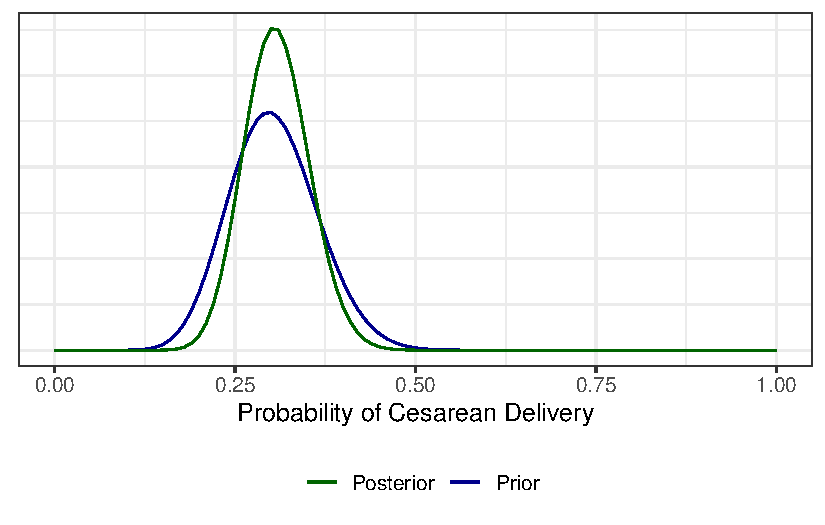
\includegraphics[width=0.8\textwidth,height=\textheight]{./images/fig-csec-comparison-1.pdf}

}

\caption{\label{fig-csec-comparison}Comparison of the prior distribution
and posterior distribution for the C-section Deliveries example given
the observed data.}

\end{figure}

\hypertarget{sec-point-estimation}{%
\chapter{Point Estimation}\label{sec-point-estimation}}

\providecommand{\norm}[1]{\lVert#1\rVert}
\providecommand{\abs}[1]{\lvert#1\rvert}
\providecommand{\iid}{\stackrel{\text{IID}}{\sim}}
\providecommand{\ind}{\stackrel{\text{Ind}}{\sim}}

\providecommand{\bm}[1]{\mathbf{#1}}
\providecommand{\bs}[1]{\boldsymbol{#1}}
\providecommand{\bbeta}{\bs{\beta}}

\providecommand{\Ell}{\mathcal{L}}
\providecommand{\indep}{\perp\negthickspace\negmedspace\perp}

Everything we could ever want to know about a parameter, given the data
we have observed, is contained in the posterior distribution. For those
very comfortable with probability theory, we may not shy away from
having an entire distribution presented to us as a way of summarizing
the information available about the parameter. However, we know there
are ways of summarizing a distribution, and often practitioners prefer
to be presented with a summary of the posterior distribution. In this
chapter, we examine methods for estimating the parameter of interest
using the posterior distribution.

\begin{tcolorbox}[enhanced jigsaw, leftrule=.75mm, coltitle=black, left=2mm, title=\textcolor{quarto-callout-tip-color}{\faLightbulb}\hspace{0.5em}{Big Idea}, breakable, toptitle=1mm, bottomtitle=1mm, colback=white, colbacktitle=quarto-callout-tip-color!10!white, titlerule=0mm, opacitybacktitle=0.6, colframe=quarto-callout-tip-color-frame, bottomrule=.15mm, arc=.35mm, opacityback=0, rightrule=.15mm, toprule=.15mm]

Estimating the parameter of interest is typically done by summarizing
the \emph{location} of the posterior distribution.

\end{tcolorbox}

A course in probability introduces us to the idea of using the mean, the
median, and/or the mode in order summarize the location of a
distribution. We can apply the same techniques to summarize the location
of the posterior distribution. The three common point estimates for a
parameter in the Bayesian framework are the posterior mean, the
posterior median, and posterior mode.

\begin{definition}[Posterior
Mean]\protect\hypertarget{def-posterior-mean}{}\label{def-posterior-mean}

The posterior mean is the average value of the parameter, given the
data:

\[E\left[\boldsymbol{\theta} \mid \mathbf{y}\right] = \int \boldsymbol{\theta} \pi(\theta \mid \mathbf{y}) d\boldsymbol{\theta}.\]

\end{definition}

We note that as the dimension of the parameter vector increases, this
could be a very difficult integral to compute. We will address this
issue in the next unit. For now, we will typically work with known
distributions and therefore known expressions for the posterior mean.

\begin{definition}[Posterior
Median]\protect\hypertarget{def-posterior-median}{}\label{def-posterior-median}

We are 50\% sure, given the data, the parameter falls below the
posterior median. Formally, the posterior median is the value \(q\) such
that

\[0.5 = \int_{-\infty}^{q} \pi(\theta \mid \mathbf{y}) d\theta.\]

\end{definition}

While closed-form solutions may exist for the posterior mean, even with
known distributions the posterior median must often be computed
numerically. This is not problematic; we are simply acknowledging that
in statistics, numerical solutions are common and are not viewed as
inferior.

\begin{definition}[Posterior
Mode]\protect\hypertarget{def-posterior-mode}{}\label{def-posterior-mode}

We think of the posterior mode as the most likely value of the
parameter, given the data. If the posterior distribution is continuous,
the posterior mode is the value of the parameter that maximizes the
posterior distribution. Formally, the posterior mode is given by

\[\arg \max_{\theta} \pi(\theta \mid \mathbf{y}).\]

\end{definition}

\begin{tcolorbox}[enhanced jigsaw, leftrule=.75mm, coltitle=black, left=2mm, title=\textcolor{quarto-callout-note-color}{\faInfo}\hspace{0.5em}{Note}, breakable, toptitle=1mm, bottomtitle=1mm, colback=white, colbacktitle=quarto-callout-note-color!10!white, titlerule=0mm, opacitybacktitle=0.6, colframe=quarto-callout-note-color-frame, bottomrule=.15mm, arc=.35mm, opacityback=0, rightrule=.15mm, toprule=.15mm]

The posterior mode only makes sense as an estimate if the posterior
distribution is unimodal.

\end{tcolorbox}

One might ask which of the three estimates is ``best.'' It depends. The
mean and median may not be representative of a ``typical'' value. The
mean is more sensitive to extreme values; the median tends to be more
stable. However, many software packages default to reporting the
posterior mean, making it a popular choice out of simplicity. Again,
regardless of which value we choose to report, we should not neglect
that we have access to the entire posterior distribution; therefore, we
are not limited by a single estimate but can provide a much richer
summary of the posterior distribution.

\begin{tcolorbox}[enhanced jigsaw, leftrule=.75mm, coltitle=black, left=2mm, title=\textcolor{quarto-callout-warning-color}{\faExclamationTriangle}\hspace{0.5em}{Warning}, breakable, toptitle=1mm, bottomtitle=1mm, colback=white, colbacktitle=quarto-callout-warning-color!10!white, titlerule=0mm, opacitybacktitle=0.6, colframe=quarto-callout-warning-color-frame, bottomrule=.15mm, arc=.35mm, opacityback=0, rightrule=.15mm, toprule=.15mm]

It is common for those first learning the Bayesian framework to confuse
the parameter being estimated with the method of estimation used. We can
use the posterior mode to estimate the mean response. We can use the
posterior mean to estimate the variance of the response. The method of
estimation (posterior mean, posterior median, or posterior mode) is
\emph{not} linked to the parameter (mean response, variance of the
response, etc.).

\end{tcolorbox}

We close this chapter by considering two examples. First, consider
Example~\ref{exm-naive-posterior}. Since the support of the posterior
includes only two values (0.246 and 0.563), the posterior mean would
necessarily take a value not in the support. The posterior median
suffers from the same limitation. The posterior mode is 0.246, since it
is the more likely value, given the data and the individual's prior
beliefs. Note, however, that we lose information by only reporting the
point estimate; we have a much richer conclusion when we report the
entire posterior distribution: we are 71.69\% sure the students are from
RHIT and 28.31\% sure the students are from ISU.

\begin{example}[C-section Deliveries
Continued]\protect\hypertarget{exm-csec-point-estimate}{}\label{exm-csec-point-estimate}

Example~\ref{exm-csec} introduced a study, a component of which includes
estimating the probability of a mother undergoing a C-section delivery
at a particular hospital.

Example~\ref{exm-csec-posterior} found the posterior distribution to be

\[\theta \mid \mathbf{x} \sim Beta\left(n + a, n\bar{x} + b\right)\]

where \(a = 17, b = 39, n = 15\) and \(n\bar{x} = 33\) given the
observed data. Estimate the rate of C-sections at the hospital given the
observed data.

\end{example}

\begin{solution}

While it may seem obvious, our estimate is based on the \emph{observed
data}; different data would lead to a different estimate. Hidden in that
statement is that our estimate is also based (at least partially) on our
prior beliefs; different prior beliefs may also lead to a different
estimate.

Since the distributional family of the posterior is well-studied (a Beta
distribution), we can make use of established properties in computing
our point estimate. In particular, we immediately have that

\[
\begin{aligned}
  E\left(\theta \mid \mathbf{x}\right)
    &= \frac{n + a}{n + a + n\bar{x} + b} = 0.308 \\
  \text{Posterior Mode} 
    &= \frac{n + a - 1}{n + a + n\bar{x} + b - 2} = 0.304.
\end{aligned}
\]

While we must compute it numerically, the posterior median is also
readily available and is given by 0.306. All three estimates are
extremely similar. Given the data, we estimate the C-section rate at the
hospital to be just over 30\% (very near the rate in the state of
Indiana).

\end{solution}

\hypertarget{sec-interval-estimation}{%
\chapter{Interval Estimation}\label{sec-interval-estimation}}

\providecommand{\norm}[1]{\lVert#1\rVert}
\providecommand{\abs}[1]{\lvert#1\rvert}
\providecommand{\iid}{\stackrel{\text{IID}}{\sim}}
\providecommand{\ind}{\stackrel{\text{Ind}}{\sim}}

\providecommand{\bm}[1]{\mathbf{#1}}
\providecommand{\bs}[1]{\boldsymbol{#1}}
\providecommand{\bbeta}{\bs{\beta}}

\providecommand{\Ell}{\mathcal{L}}
\providecommand{\indep}{\perp\negthickspace\negmedspace\perp}

The previous chapter considered a single point estimate for the
parameter of interest. However, this ignores the fact that there is
variability in these estimates. The distribution itself tells us the
parameter is more likely to fall in some regions than others. In
response, we consider providing a range of plausible values for the
parameter and quantifying our belief that the parameter falls in that
range. This is the contrast between point and interval estimation.

\begin{definition}[Point
Estimation]\protect\hypertarget{def-point-estimation}{}\label{def-point-estimation}

Point estimation is the process of estimating a parameter with a single
statistic. This is like trying to hit an infinitesimally small target
with a dart.

\end{definition}

\begin{definition}[Interval
Estimation]\protect\hypertarget{def-interval-estimation}{}\label{def-interval-estimation}

Interval estimation is the process of estimating a parameter with a
range of values. This is like trying to capture a target with a ring.

\end{definition}

Regardless of which method we use, both are estimates, and both depend
on the posterior distribution. That is, both are statements about the
parameter given the observed data and our prior beliefs. As there were
various techniques for constructing a point estimate, there are various
techniques for an interval estimate; the most common of these is the
credible interval.

\begin{definition}[Credible
Interval]\protect\hypertarget{def-credible-interval}{}\label{def-credible-interval}

A \(100c\)\% credible interval is an interval \((a, b)\) such that

\[Pr(a \leq \theta \leq b \mid \mathbf{y}) = \int_{a}^{b} \pi(\theta \mid \mathbf{y})d\theta = c.\]

\end{definition}

\begin{tcolorbox}[enhanced jigsaw, leftrule=.75mm, coltitle=black, left=2mm, title=\textcolor{quarto-callout-warning-color}{\faExclamationTriangle}\hspace{0.5em}{Warning}, breakable, toptitle=1mm, bottomtitle=1mm, colback=white, colbacktitle=quarto-callout-warning-color!10!white, titlerule=0mm, opacitybacktitle=0.6, colframe=quarto-callout-warning-color-frame, bottomrule=.15mm, arc=.35mm, opacityback=0, rightrule=.15mm, toprule=.15mm]

For those who have had a previous statistics course taught from the
classical Frequentist perspective, this seems to mirror a confidence
interval, but the interpretation is completely different. Since
probability is used to quantify subjective beliefs, notice that the
credible interval allows us to say that we are \(100c\)\% sure the
parameter falls in this range, given the data.

Since we are working from a subjective interpretation of probability, we
do not need to appeal to repeated sampling (like a Frequentist would).
In fact, since a parameter is a fixed, unknown quantity, any probability
statement is illogical from a Frequentist perspective. However, from the
Bayesian perspective, the posterior quantifies our uncertainty about the
parameter, and therefore the credible interval is simply summarizing
this uncertainty. We can now say, based on the data observed (however
much or little we have), we are \(100c\)\% sure the parameter falls in
this interval.

\end{tcolorbox}

\begin{tcolorbox}[enhanced jigsaw, leftrule=.75mm, coltitle=black, left=2mm, title=\textcolor{quarto-callout-note-color}{\faInfo}\hspace{0.5em}{Note}, breakable, toptitle=1mm, bottomtitle=1mm, colback=white, colbacktitle=quarto-callout-note-color!10!white, titlerule=0mm, opacitybacktitle=0.6, colframe=quarto-callout-note-color-frame, bottomrule=.15mm, arc=.35mm, opacityback=0, rightrule=.15mm, toprule=.15mm]

There is no one unique credible interval for a parameter.

\end{tcolorbox}

Since there are infinitely many regions which contain \(100c\)\% of the
posterior distribution, there are infinitely many credible intervals we
could provide. In order to provide some level of continuity between
applications, we tend to gravitate to one of two types of intervals
which have nice properties.

\begin{definition}[Equal-Tailed Credible
Interval]\protect\hypertarget{def-equal-tail-interval}{}\label{def-equal-tail-interval}

The equal-tailed credible interval, which is probably the most commonly
used in practice, chooses endpoints such that

\[Pr(\theta < a \mid \mathbf{y}) = \frac{1-c}{2} = Pr(\theta > b \mid \mathbf{y}).\]

\end{definition}

As the name implies, an equal-tailed credible interval places the same
probability in each tail; we are taking the middle \(100c\)\% of the
posterior distribution.

An equal-tailed interval is easy, but it may not always be the most
intuitive interval.
Figure~\ref{fig-interval-estimation-compare-intervals} compares two
potential 90\% credible intervals for a hypothetical posterior
distribution. Observe that the equal-tailed interval removes the bottom
5\% of the distribution; while this band is narrow, it represents values
which correspond to the highest posterior density values. It seems
intuitive that we would want to choose the narrowest credible interval
which still retains the same area under the curve, as illustrated in the
second panel of Figure~\ref{fig-interval-estimation-compare-intervals}.

\begin{figure}

{\centering 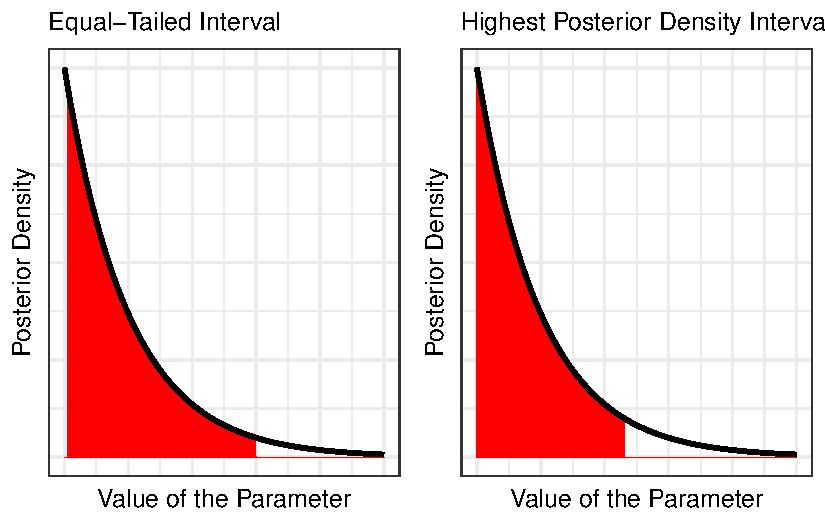
\includegraphics[width=0.8\textwidth,height=\textheight]{./images/fig-interval-estimation-compare-intervals-1.pdf}

}

\caption{\label{fig-interval-estimation-compare-intervals}Comparison of
two 90\% credible intervals for a hypothetical posterior distribution.}

\end{figure}

\begin{definition}[Highest Density
Interval]\protect\hypertarget{def-hdi}{}\label{def-hdi}

The highest density interval, often called an HDI or HPD (for highest
posterior density), chooses the endpoints such that the interval is as
short as possible.

When the density is unimodal, this can be accomplished by choosing the
endpoints \(a\) and \(b\) such that

\[\pi(\theta \mid \mathbf{y}) \mid_{\theta = a} = \pi(\theta \mid \mathbf{y}) \mid_{\theta = b}\]

and

\[\int_{a}^{b} \pi(\theta \mid \mathbf{y} d\theta = c.\]

\end{definition}

\begin{tcolorbox}[enhanced jigsaw, leftrule=.75mm, coltitle=black, left=2mm, title=\textcolor{quarto-callout-note-color}{\faInfo}\hspace{0.5em}{Note}, breakable, toptitle=1mm, bottomtitle=1mm, colback=white, colbacktitle=quarto-callout-note-color!10!white, titlerule=0mm, opacitybacktitle=0.6, colframe=quarto-callout-note-color-frame, bottomrule=.15mm, arc=.35mm, opacityback=0, rightrule=.15mm, toprule=.15mm]

If the posterior distribution is multimodal, then the highest density
interval is actually a \emph{region} as it will likely involve two
disjoint intervals.

\end{tcolorbox}

\begin{tcolorbox}[enhanced jigsaw, leftrule=.75mm, coltitle=black, left=2mm, title=\textcolor{quarto-callout-warning-color}{\faExclamationTriangle}\hspace{0.5em}{Warning}, breakable, toptitle=1mm, bottomtitle=1mm, colback=white, colbacktitle=quarto-callout-warning-color!10!white, titlerule=0mm, opacitybacktitle=0.6, colframe=quarto-callout-warning-color-frame, bottomrule=.15mm, arc=.35mm, opacityback=0, rightrule=.15mm, toprule=.15mm]

Most software that computes an HDI assumes the poterior distribution is
unimodal.

\end{tcolorbox}

Suppose we have a \(100c\)\% credible interval \((a, b)\) for some
parameter \(\theta\), but we are interested in a transformation of the
parameter \(\eta = g(\theta)\). We can develop a \(100c\)\% credible
interval for \(\eta\) by applying the same transformation to each
endpoint of the interval for \(\theta\). That is,
\(\left(g(a), g(b)\right)\) will be a \(100c\)\% credible interval for
the parameter \(\eta\) given the data.

While we can guarantee that \(\left(g(a), g(b)\right)\) is a \(100c\)\%
credible interval, it will in general \textbf{not} be the HDI for
\(\eta\), even if \((a, b)\) is the HDI for \(\theta\).

\begin{example}[C-section Deliveries
Continued]\protect\hypertarget{exm-csec-interval-estimate}{}\label{exm-csec-interval-estimate}

Example~\ref{exm-csec} introduced a study, a component of which includes
estimating the probability of a mother undergoing a C-section delivery
at a particular hospital.

Example~\ref{exm-csec-posterior} found the posterior distribution to be

\[\theta \mid \mathbf{x} \sim Beta\left(n + a, n\bar{x} + b\right)\]

where \(a = 17, b = 39, n = 15\) and \(n\bar{x} = 33\) given the
observed data. Estimate the rate of C-sections at the hospital given the
observed data.

\end{example}

\begin{solution}

Example~\ref{exm-csec-point-estimate} developed point estimates of the
unknown parameter given the observed data (and prior beliefs). Here, we
consider an interval estimate. To compute an equal-tailed interval, we
must choose the values of \(s\) and \(t\) such that

\[
\begin{aligned}
  0.025 &= \int_{0}^{s} \frac{\Gamma(32 + 72)}{\Gamma(32) \Gamma(72)} \theta^{32 - 1} (1 - \theta)^{72 - 1} d\theta \\
  0.025 &= \int_{t}^{1} \frac{\Gamma(32 + 72)}{\Gamma(32) \Gamma(72)} \theta^{32 - 1} (1 - \theta)^{72 - 1} d\theta. \\
\end{aligned}
\]

Solving this system numerical gives the interval \((0.223, 0.399)\). We
are 95\% sure, given the data, the rate of C-sections at the hospital is
between 22.3\% and 39.9\%. Given that the posterior distribution is
unimodal and nearly symmetric, we would expect the HDI to be very
similar to the equal-tailed interval.

\end{solution}

\hypertarget{sec-prediction}{%
\chapter{Prediction}\label{sec-prediction}}

\providecommand{\norm}[1]{\lVert#1\rVert}
\providecommand{\abs}[1]{\lvert#1\rvert}
\providecommand{\iid}{\stackrel{\text{IID}}{\sim}}
\providecommand{\ind}{\stackrel{\text{Ind}}{\sim}}

\providecommand{\bm}[1]{\mathbf{#1}}
\providecommand{\bs}[1]{\boldsymbol{#1}}
\providecommand{\bbeta}{\bs{\beta}}

\providecommand{\Ell}{\mathcal{L}}
\providecommand{\indep}{\perp\negthickspace\negmedspace\perp}

Previous chapters have focused on making a statement about the parameter
given the data. However, researchers are often interested in using the
data to predict what might occur in the future. Hopefully, by now you
realize that within the Bayesian framework, we are never interested
\emph{solely} in a point estimate. So, when we say we are interested in
``prediction,'' we mean we are interested in characterizing our
uncertainty in a future value given the data we have observed. As this
statement is not directly about the parameter, the posterior
distribution does \textbf{not} contain the relevant information; but, it
can be used to derive the distribution that is relevant.

Imagine we have not yet collected data. Given only our prior beliefs,
how might we characterize a future observation (one not yet observed)?
We may not know what value a future observation will take, but we have
some sense of the process that will generate it if we have posited a
likelihood to describe the data generating process.

In probability, we routinely use the distribution to characterize future
values each time we answered a question like ``what is the probability
we will observe a value between \(a\) and \(b\)?'' It is therefore
intuitive that we might turn toward the likelihood
\(f(\mathbf{y} \mid \theta)\) to describe the variability in data that
has not yet been observed. Of course, this highlights the difference
between probability and statistics --- in probability, we always knew
the value of \(\theta\), but in statistics, we do not. Without a value
of \(\theta\) to plug into the density, we are unable to use it to
compute probabilities about future observations (or, more precisely, any
probabilities we computed would be a function of the unknown parameter).

This is where our prior beliefs come into play. While we do not know the
value of \(\theta\), we do have some prior beliefs about it, and these
are captured in the prior distribution. The Bayesian framework proposes
marginalizing out the parameter --- essentially taking a weighted
average over all possible values it could be. What results is not a
single value, but a distribution of values known as the prior predictive
distribution.

\begin{definition}[Prior Predictive
Distribution]\protect\hypertarget{def-prior-predictive-distribution}{}\label{def-prior-predictive-distribution}

The prior predictive distribution is the marginal distribution of the
response(s) prior to observing any data:

\[m(\mathbf{y}) = \int f(\mathbf{y} \mid \theta) \pi(\theta) d\theta.\]

The distribution marginalizes the parameter out of the likelihood using
the beliefs from the prior distribution.

\end{definition}

\begin{tcolorbox}[enhanced jigsaw, leftrule=.75mm, coltitle=black, left=2mm, title=\textcolor{quarto-callout-note-color}{\faInfo}\hspace{0.5em}{Note}, breakable, toptitle=1mm, bottomtitle=1mm, colback=white, colbacktitle=quarto-callout-note-color!10!white, titlerule=0mm, opacitybacktitle=0.6, colframe=quarto-callout-note-color-frame, bottomrule=.15mm, arc=.35mm, opacityback=0, rightrule=.15mm, toprule=.15mm]

The prior predictive distribution is the denominator in Bayes Theorem.

\end{tcolorbox}

While rarely used directly, the prior predictive distribution provides a
way of characterizing our uncertainty in future observations based
solely on our beliefs about \(\theta\) prior to observing any data.

\begin{tcolorbox}[enhanced jigsaw, leftrule=.75mm, coltitle=black, left=2mm, title=\textcolor{quarto-callout-tip-color}{\faLightbulb}\hspace{0.5em}{Big Idea}, breakable, toptitle=1mm, bottomtitle=1mm, colback=white, colbacktitle=quarto-callout-tip-color!10!white, titlerule=0mm, opacitybacktitle=0.6, colframe=quarto-callout-tip-color-frame, bottomrule=.15mm, arc=.35mm, opacityback=0, rightrule=.15mm, toprule=.15mm]

We can describe our beliefs about future values of the response by
marginalizing the parameter out of the likelihood.

\end{tcolorbox}

Of course, we will eventually collect data, and we would like to take
this knowledge into account. After observing the data, the parameter
remains unknown; however, our beliefs about the parameter are updated
(and are captured in the posterior distribution). We want to marginalize
the parameter out of the likelihood while accounting for these updated
beliefs.

We consider swapping out the role of the prior distribution in
Definition~\ref{def-prior-predictive-distribution} with the posterior
distribution. The result is the posterior predictive distribution.

\begin{definition}[Posterior Predictive
Distribution]\protect\hypertarget{def-posterior-predictive-distribution}{}\label{def-posterior-predictive-distribution}

Let \(\mathbf{Y}^*\) represent a collection of \(m\) \emph{future}
observations. The distribution of these future observations given the
observed data \(\mathbf{Y}\) (of length \(n\)), called the posterior
predictive distribution, is given by

\[\pi\left(\mathbf{y}^* \mid \mathbf{y}\right) = \int f\left(\mathbf{y}^* \mid \theta\right) \pi(\theta \mid \mathbf{y}) d\theta.\]

\end{definition}

While this definition is correct, its derivation requires some
additional constraints on the data generating process. We present the
derivation below primarily to combat any misconceptions about what is
happening in the integration above.

\hypertarget{derivation-of-the-posterior-predictive}{%
\section{Derivation of the Posterior
Predictive}\label{derivation-of-the-posterior-predictive}}

Let \(\mathbf{Y}^*\) denote a collection of \(m\) future (or new)
observations not yet observed. This is distinguished from the collection
of \(n\) observations we have already made \(\mathbf{Y}\). We impose the
following two conditions/assumptions on the data generating process:

\begin{itemize}
\tightlist
\item
  Given the value of the parameter, the likelihood of \(\mathbf{Y}^*\)
  has the same form as the likelihood of of the observed data
  \(\mathbf{Y}\).
\item
  Given the value of the parameter, the observed data \(\mathbf{Y}\) is
  \emph{independent} of the new observations \(\mathbf{Y}^*\).
\end{itemize}

The first condition essentially states the data generated under one
process should only be used to predict data generated from the same
process. Intuitively, when we collect data, it can only inform us about
the process from which it was generated. Therefore, our future
observations are always related in some way to the likelihood, as that
models the data generating process of interest.

The second condition extends the concept of independence presented in a
typical probability course. This is \emph{conditional independence}.

\begin{definition}[Conditional
Independence]\protect\hypertarget{def-conditional-independence}{}\label{def-conditional-independence}

Two random variables \(X\) and \(Y\) are said to be independent,
conditional on (or ``given'') \(Z\) if, and only if,

\[f_{(X,Y) \mid Z} (x, y \mid z) = f_{X \mid Z}(x \mid z) f_{Y \mid Z}(y \mid z).\]

\end{definition}

Conditional independence is common in statistical theory. Two random
quantities are somehow related, but given an additional piece of
information become independent. That is, all the information about the
relationship between \(X\) and \(Y\) is contained in the random variable
\(Z\).

Returning to the stated condition, we are saying that the only thing the
new and old observations have in common is the data generating process;
once we know the quantities that govern this process (the parameters),
then we can gain no further knowledge about the new observations from
the old observations. That is, if someone told you what the parameters
were, there would be no need to collect data --- you would know
everything possible for predicting a future observation. So, the data
observed is only useful in that it informs our beliefs about the unknown
parameters.

\begin{tcolorbox}[enhanced jigsaw, leftrule=.75mm, coltitle=black, left=2mm, title=\textcolor{quarto-callout-tip-color}{\faLightbulb}\hspace{0.5em}{Big Idea}, breakable, toptitle=1mm, bottomtitle=1mm, colback=white, colbacktitle=quarto-callout-tip-color!10!white, titlerule=0mm, opacitybacktitle=0.6, colframe=quarto-callout-tip-color-frame, bottomrule=.15mm, arc=.35mm, opacityback=0, rightrule=.15mm, toprule=.15mm]

The data observed informs our beliefs about the parameters in the data
generating process. It is only through what the data tells us about the
parameters that the data is useful in predicting a future observation.

\end{tcolorbox}

We are now prepared to derive the posterior predictive distribution.
Recall that a marginal distribution can be constructed by integrating
over the other elements of a joint distribution. For example,

\[f\left(\mathbf{y}^*\right) = \int f\left(\mathbf{y}^*, \theta\right) d\theta.\]

Here, we have considered the joint distribution of the new data
\(\mathbf{Y}^*\) and the parameter \(\theta\), then integrated over
\(\theta\). This strategy works even when we are carrying a conditional
term through. That is, we have that

\begin{equation}\protect\hypertarget{eq-post-pred-step1}{}{\pi\left(\mathbf{y}^* \mid \mathbf{y}\right) = \int f\left(\mathbf{y}^*, \theta \mid \mathbf{y}\right) d\theta.}\label{eq-post-pred-step1}\end{equation}

Here, we have considered the joint distribution of the new data
\(\mathbf{Y}^*\) and the parameter \(\theta\) (conditional on the
observed data), then integrated over \(\theta\). This statement would
have been true for any choice of random variable, but using the
parameter allows us to make use of the information we have collected
through the observed data.

We now recall that any joint distribution can be written as the product
of a conditional distribution and a marginal distribution; this is true
even if we are already conditioning on another random variable. This
gives

\begin{equation}\protect\hypertarget{eq-post-pred-step2}{}{f(\mathbf{y}^*, \theta \mid \mathbf{y}) = f(\mathbf{y}^* \mid \mathbf{y}, \theta) \pi(\theta \mid \mathbf{y}).}\label{eq-post-pred-step2}\end{equation}

Substituting Equation~\ref{eq-post-pred-step2} into
Equation~\ref{eq-post-pred-step1}, we now have that the posterior
predictive distribution is given by

\begin{equation}\protect\hypertarget{eq-post-pred-step3}{}{\pi\left(\mathbf{y}^* \mid \mathbf{y}\right) = \int f(\mathbf{y}^* \mid \mathbf{y}, \theta) \pi(\theta \mid \mathbf{y}) d\theta.}\label{eq-post-pred-step3}\end{equation}

We now make use of conditional independence. We now consider the term
\(f(\mathbf{y}^* \mid \mathbf{y}, \theta)\) inside the integral. By the
definition of a conditional density, we have

\[f(\mathbf{y}^* \mid \mathbf{y}, \theta) = \frac{f(\mathbf{y}^*, \mathbf{y} \mid \theta)}{f(\mathbf{y} \mid \theta)}.\]

However, if we are willing to assume that \(\mathbf{Y}^*\) is
independent of \(\mathbf{Y}\) given \(\theta\), then the numerator
becomes the product of \(f(\mathbf{y}^* \mid \theta)\) and
\(f(\mathbf{y} \mid \theta)\), meaning we have that
\(f(\mathbf{y}^* \mid \mathbf{y}, \theta) = f(\mathbf{y}^* \mid \theta)\)
under conditional independence. Substituting in this expression into
Equation~\ref{eq-post-pred-step3} gives the posterior predictive
distribution in Definition~\ref{def-posterior-predictive-distribution}.

\hypertarget{summary}{%
\section{Summary}\label{summary}}

Once you have the posterior predictive distribution, you have everything
there is to know about future observations given the data observed.
Further, the posterior predictive distribution can be summarized just
like any other distribution. Summarizing the location (mean, median,
mode) would result in point estimates for future observations.
Alternatively, we can construct interval estimates by defining a range
for which the future observations would fall with some known
probability.

\begin{tcolorbox}[enhanced jigsaw, leftrule=.75mm, coltitle=black, left=2mm, title=\textcolor{quarto-callout-warning-color}{\faExclamationTriangle}\hspace{0.5em}{Warning}, breakable, toptitle=1mm, bottomtitle=1mm, colback=white, colbacktitle=quarto-callout-warning-color!10!white, titlerule=0mm, opacitybacktitle=0.6, colframe=quarto-callout-warning-color-frame, bottomrule=.15mm, arc=.35mm, opacityback=0, rightrule=.15mm, toprule=.15mm]

Keep in mind that we have switched our focus. We are now focused on a
possible data point, not a parameter. Therefore, the support of the
posterior predictive need not be the same as the support of the
posterior distribution.

\end{tcolorbox}

\begin{example}[C-section Deliveries
Continued]\protect\hypertarget{exm-csec-prediction}{}\label{exm-csec-prediction}

Example~\ref{exm-csec} introduced a study, a component of which includes
estimating the probability of a mother undergoing a C-section delivery
at a particular hospital.

Example~\ref{exm-csec-posterior} found the posterior distribution to be

\[\theta \mid \mathbf{x} \sim Beta\left(n + a, n\bar{x} + b\right)\]

where \(a = 17, b = 39, n = 15\) and \(n\bar{x} = 33\) given the
observed data. Suppose we are interested in adding a 16-th patient to
our survey; predict the number of vaginal deliveries we should expect
before we observe a C-section.

\end{example}

\begin{solution}

We are interested in predicting a new \emph{response} given the observed
data. Following the discussion in the derivation of the posterior
predictive distribution, it makes sense that we would assume the density
of this new response follows the same distribution as the observed data.
In particular, if \(Y\) represents the future observation, then

\[f(y \mid \theta) = \theta (1 - \theta)^y\]

since each observed value (previously denoted by \(X_i\)) was modeled as
a random variate from a Geometric distribution. Applying
Definition~\ref{def-posterior-predictive-distribution}, we have that the
posterior predictive distribution is given by

\[
\begin{aligned}
  \pi(y \mid \mathbf{x})
    &= \int f\left(y \mid \theta\right) \pi(\theta \mid \mathbf{x}) d\theta \\
    &= \int \theta (1 - \theta)^y \frac{\Gamma(n + a + n\bar{x} + b)}{\Gamma(n + a) \Gamma(n\bar{x} + b)} \theta^{n + a - 1} (1 - \theta)^{n\bar{x} + b - 1} d\theta \\
    &= \frac{\Gamma(n + a + n\bar{x} + b)}{\Gamma(n + a) \Gamma(n\bar{x} + b)} \int \theta^{n + a + 1 - 1} (1 - \theta)^{n\bar{x} + b + y - 1} d\theta. 
\end{aligned}
\]

Notice that the integrand is the kernel of a Beta distribution;
therefore, we can multiply and divide by the appropriate scaling terms.
This gives

\[
\begin{aligned}
  \pi(y \mid \mathbf{x})
    &= \frac{\Gamma(n + a + n\bar{x} + b)}{\Gamma(n + a) \Gamma(n\bar{x} + b)} \int \theta^{n + a + 1 - 1} (1 - \theta)^{n\bar{x} + b + y - 1} d\theta \\
    &= \frac{\Gamma(n + a + n\bar{x} + b)}{\Gamma(n + a) \Gamma(n\bar{x} + b)} \frac{\Gamma(n + a + 1) \Gamma(n\bar{x} + b + y)}{\Gamma(n + a + n\bar{x} + b + 1 + y)} \\
    &\qquad \cdot \int \frac{\Gamma(n + a + n\bar{x} + b + 1 + y)}{\Gamma(n + a + 1) \Gamma(n\bar{x} + b + y)} \theta^{n + a + 1 - 1} (1 - \theta)^{n\bar{x} + b + y - 1} d\theta \\
    &= \frac{\Gamma(n + a + n\bar{x} + b)}{\Gamma(n + a) \Gamma(n\bar{x} + b)} \frac{\Gamma(n + a + 1) \Gamma(n\bar{x} + b + y)}{\Gamma(n + a + n\bar{x} + b + 1 + y)}.
\end{aligned}
\]

We are not meant to recognize this distribution. However, we can work
with it. We must keep in mind the warning, however, given just prior to
this example --- the support of this distribution is non-negative
integers, not the interval \((0, 1)\).

Again, prediction is not about saying how many vaginal births we
\emph{will} see before the next C-section; it is really about
quantifying our uncertainty in the various possibilities. For example,
given the data observed, we are 30.8\% sure that the very next birth
will be a C-section, since

\[Pr(Y = 1 \mid \mathbf{x}) = \frac{\Gamma(32 + 72)}{\Gamma(32) \Gamma(72)} \frac{\Gamma(32 + 1) \Gamma(72 + 0)}{\Gamma(32 + 72 + 1 + 0)} = 0.308.\]

Similarly, we are 88.3\% sure that we will not experience more than 5
vaginal births before the next C-section, since

\[Pr(Y \leq 5 \mid \mathbf{x}) \sum_{u=0}^{5} Pr(Y = u \mid \mathbf{x}) = 1 - \sum_{u=0}^{5} \frac{\Gamma(32 + 72)}{\Gamma(32) \Gamma(72)} \frac{\Gamma(32 + 1) \Gamma(72 + u)}{\Gamma(32 + 72 + 1 + u)} = 0.883.\]

However, if we would like to provide a single point estimate instead of
probabilities of specific responses, we might report that, given the
data, \emph{on average}, we expect to see 2.32 vaginal deliveries before
the next C-section since

\[E\left(Y \mid \mathbf{x}\right) = \sum_{u=0}^{\infty} u Pr(Y = u \mid \mathbf{x}) = 2.32.\]

\end{solution}

\hypertarget{sec-hypothesis-testing}{%
\chapter{Hypothesis Testing}\label{sec-hypothesis-testing}}

\providecommand{\norm}[1]{\lVert#1\rVert}
\providecommand{\abs}[1]{\lvert#1\rvert}
\providecommand{\iid}{\stackrel{\text{IID}}{\sim}}
\providecommand{\ind}{\stackrel{\text{Ind}}{\sim}}

\providecommand{\bm}[1]{\mathbf{#1}}
\providecommand{\bs}[1]{\boldsymbol{#1}}
\providecommand{\bbeta}{\bs{\beta}}

\providecommand{\Ell}{\mathcal{L}}
\providecommand{\indep}{\perp\negthickspace\negmedspace\perp}

We have considered both estimation and prediction at this point. The
third type of question often asked by researchers is which model (out of
some pre-defined set) is most supported by the data. As with previous
estimation and prediction, the Bayesian framework seeks to characterize
the evidence for each model, given the data.

\begin{tcolorbox}[enhanced jigsaw, leftrule=.75mm, coltitle=black, left=2mm, title=\textcolor{quarto-callout-warning-color}{\faExclamationTriangle}\hspace{0.5em}{Warning}, breakable, toptitle=1mm, bottomtitle=1mm, colback=white, colbacktitle=quarto-callout-warning-color!10!white, titlerule=0mm, opacitybacktitle=0.6, colframe=quarto-callout-warning-color-frame, bottomrule=.15mm, arc=.35mm, opacityback=0, rightrule=.15mm, toprule=.15mm]

For those who are familiar with a classical Frequentist approach to
hypothesis testing, you will note that the above language is
fundamentally different than the Frequentist perspective. The
Frequentist perspective does not allow us to characterize the
``evidence'' for the null hypothesis, and it would certainly never allow
us to quantify the probability of a hypothesis being true.

\end{tcolorbox}

You may recall that for the Naive Classification of College Students
example (Example~\ref{exm-naive}), we derived the following posterior
distribution (see Equation~\ref{eq-naive-posterior}):

\[\pi(\theta \mid y) = (0.7169)\delta(\theta - 0.246) + (0.2831)\delta(\theta - 0.563).\]

This posterior distribution followed from learning 3 of the 10 students
identify as female combined with the prior belief that there was a 60\%
chance the students were from ISU.

This example is nice for illustrating hypothesis testing because baked
into the problem were essentially two hypotheses:

\[H_0: \theta = 0.246 \qquad \text{vs.} \qquad H_1: \theta = 0.563\]

where the null hypothesis represents the belief that the students are
from Rose-Hulman (where 24.6\% of students identify as female) and the
alterntative hypothesis represents the belief that the students are from
ISU (where 56.3\% of students identify as female). In this example, each
hypothesis specifies a single value for the parameter; in general, each
hypothesis could specify a region for the parameter. That is, we are
generally interested in testing

\[H_0: \theta \in \Theta_0 \qquad \text{vs.} \qquad H_1: \theta \in \Theta_1.\]

While not a requirement, in practice \(\Theta_0\) and \(\Theta_1\) are
typically mutually exclusive sets which form a partition of the
parameter space.

\begin{tcolorbox}[enhanced jigsaw, leftrule=.75mm, coltitle=black, left=2mm, title=\textcolor{quarto-callout-note-color}{\faInfo}\hspace{0.5em}{Note}, breakable, toptitle=1mm, bottomtitle=1mm, colback=white, colbacktitle=quarto-callout-note-color!10!white, titlerule=0mm, opacitybacktitle=0.6, colframe=quarto-callout-note-color-frame, bottomrule=.15mm, arc=.35mm, opacityback=0, rightrule=.15mm, toprule=.15mm]

Nothing prohibits us from having more than two hypotheses in this
framework, and nothing requires the hypotheses form a partition of the
parameter space.

\end{tcolorbox}

Under the Bayesian framework, it is straightforward to compute
probabilities of the form ``the probability \(H_j\) is true given the
data observed.''

\begin{tcolorbox}[enhanced jigsaw, leftrule=.75mm, coltitle=black, left=2mm, title=\textcolor{quarto-callout-note-color}{\faInfo}\hspace{0.5em}{Note}, breakable, toptitle=1mm, bottomtitle=1mm, colback=white, colbacktitle=quarto-callout-note-color!10!white, titlerule=0mm, opacitybacktitle=0.6, colframe=quarto-callout-note-color-frame, bottomrule=.15mm, arc=.35mm, opacityback=0, rightrule=.15mm, toprule=.15mm]

Under the classical Frequentist perspective, the probability a
hypothesis is true is nonsensical; however, under the Bayesian approach,
we are using probability simply to characterize our uncertainty about
the statement.

\end{tcolorbox}

For the Naive Classification of College Students, the posterior
naturally allows us to address the hypothesis. Notice that

\[
\begin{aligned}
  Pr\left(H_0 \mid y\right) &= Pr(\theta = 0.246 \mid y) = 0.7169 \\
  Pr\left(H_1 \mid y\right) &= Pr(\theta = 0.563 \mid y) = 0.2831.
\end{aligned}
\]

That is, after observing the data, we believe it is much more likely the
the students are from Rose-Hulman than from ISU.

\begin{tcolorbox}[enhanced jigsaw, leftrule=.75mm, coltitle=black, left=2mm, title=\textcolor{quarto-callout-note-color}{\faInfo}\hspace{0.5em}{Note}, breakable, toptitle=1mm, bottomtitle=1mm, colback=white, colbacktitle=quarto-callout-note-color!10!white, titlerule=0mm, opacitybacktitle=0.6, colframe=quarto-callout-note-color-frame, bottomrule=.15mm, arc=.35mm, opacityback=0, rightrule=.15mm, toprule=.15mm]

Again, contrasting the conclusion in the Bayesian framework with a
classical Frequentist framework, we are saying that the data is
convincing us to believe the null hypothesis over the alternative. The
idea of ``accepting'' the null hypothesis in the classical Frequentist
framework is heretical.

\end{tcolorbox}

In addition to computing the probability of each hypothesis, we can
compute how much more likely we are to believe the students are from
Rose-Hulman compared to believing they are from ISU:

\[\frac{Pr\left(H_0 \mid y\right)}{Pr\left(H_1 \mid y\right)} = 2.53;\]

that is, given the data, we believe it is 2.53 times more likely that
the students are from Rose-Hulman than from ISU. This is known as the
posterior odds.

\begin{definition}[Posterior
Odds]\protect\hypertarget{def-posterior-odds}{}\label{def-posterior-odds}

Let \(H_j\) denote the hypothesis that \(\theta \in \Theta_j\) for some
region \(\Theta_j\). Then, the posterior odds \emph{in favor of} \(H_j\)
is given by

\[\frac{Pr\left(\theta \in \Theta_j \mid \mathbf{y}\right)}{Pr\left(\theta \notin \Theta_j \mid \mathbf{y}\right)}.\]

\end{definition}

\begin{tcolorbox}[enhanced jigsaw, leftrule=.75mm, coltitle=black, left=2mm, title=\textcolor{quarto-callout-note-color}{\faInfo}\hspace{0.5em}{Note}, breakable, toptitle=1mm, bottomtitle=1mm, colback=white, colbacktitle=quarto-callout-note-color!10!white, titlerule=0mm, opacitybacktitle=0.6, colframe=quarto-callout-note-color-frame, bottomrule=.15mm, arc=.35mm, opacityback=0, rightrule=.15mm, toprule=.15mm]

When there are only two hypotheses, and they partition the parameter
space, then the posterior odds captures how strongly we favor one
hypothesis over the other given the data.

\end{tcolorbox}

The posterior odds is useful, but it only suggests how we feel after we
have observed the data. We may be more interested in how much the data
\emph{impacted} our prior beliefs. For example, if the data simply
confirmed our beliefs, that is not nearly as extraordinary as the data
completely reversing our beliefs. The Bayes Factor captures this impact.

\begin{definition}[Bayes
Factor]\protect\hypertarget{def-bayes-factor}{}\label{def-bayes-factor}

A measure of how the observed data \emph{alters} your prior beliefs
about a hypothesis. Let \(H_j\) denote the hypothesis that
\(\theta \in \Theta_j\) for some region \(\Theta_j\). The Bayes Factor
\emph{in favor of} \(H_j\) is the ratio of the posterior odds in favor
of \(H_j\) to the prior odds in favor of \(H_j\):

\[BF_j = \left(\frac{Pr\left(\theta \in \Theta_j \mid \mathbf{y}\right)}{Pr\left(\theta \notin \Theta_j \mid \mathbf{y}\right)}\right)\left(\frac{Pr\left(\theta \notin \Theta_j\right)}{Pr\left(\theta \in \Theta_j\right)}\right).\]

\end{definition}

\begin{tcolorbox}[enhanced jigsaw, leftrule=.75mm, coltitle=black, left=2mm, title=\textcolor{quarto-callout-note-color}{\faInfo}\hspace{0.5em}{Note}, breakable, toptitle=1mm, bottomtitle=1mm, colback=white, colbacktitle=quarto-callout-note-color!10!white, titlerule=0mm, opacitybacktitle=0.6, colframe=quarto-callout-note-color-frame, bottomrule=.15mm, arc=.35mm, opacityback=0, rightrule=.15mm, toprule=.15mm]

Some prefer to report the logarithm of the Bayes Factor, as it is a
quantity that is easier to work with in theoretical derivations.

\end{tcolorbox}

Keep in mind, the Bayesian framework is about quantifying our
uncertainty about the unknown parameters. The Bayes Factor measures how
that uncertainty has been impacted by the observed data. Two independent
papers made recommendations for how to interpret a Bayes Factor;
however, we should remember that these are simply ``rules of thumb.''

\hypertarget{tbl-bayes-factor}{}
\begin{longtable}[]{@{}lcc@{}}
\caption{\label{tbl-bayes-factor}Rules of thumb for interpreting the
Bayes Factor as suggested by Jeffreys and Kass and
Raftery.}\tabularnewline
\toprule\noalign{}
Strength of Evidence & Jeffreys' Scale & Kass and Raftery Scale \\
\midrule\noalign{}
\endfirsthead
\toprule\noalign{}
Strength of Evidence & Jeffreys' Scale & Kass and Raftery Scale \\
\midrule\noalign{}
\endhead
\bottomrule\noalign{}
\endlastfoot
Weak & \(0 \leq \log_{10}(BF) < 0.5\) & \(0 \leq \log(BF) < 1\) \\
Substantial & \(0.5 \leq \log_{10}(BF) < 1\) &
\(1 \leq \log(BF) < 3\) \\
Strong & \(1 \leq \log_{10}(BF) < 2\) & \(3 \leq \log(BF) < 5\) \\
Decisive & \(2 \leq \log_{10}(BF)\) & \(5 \leq \log(BF)\) \\
\end{longtable}

\begin{tcolorbox}[enhanced jigsaw, leftrule=.75mm, coltitle=black, left=2mm, title=\textcolor{quarto-callout-warning-color}{\faExclamationTriangle}\hspace{0.5em}{Warning}, breakable, toptitle=1mm, bottomtitle=1mm, colback=white, colbacktitle=quarto-callout-warning-color!10!white, titlerule=0mm, opacitybacktitle=0.6, colframe=quarto-callout-warning-color-frame, bottomrule=.15mm, arc=.35mm, opacityback=0, rightrule=.15mm, toprule=.15mm]

Take caution when interpreting a Bayes Factor; it quantifies the degree
to which the data altered your prior beliefs. It is possible to have a
really small Bayes Factor in favor of a hypothesis and yet
simultaneously believe overwhelmingly in that hypothesis given the data;
the small Bayes Factor simply implies that you believed in that
hypothesis before collecting the data as well. Conversely, it is
possible to have a really large Bayes Factor in favor of a hypothesis
and yet simultaneously not distinguish between that hypothesis and
another given the data; the large Bayes Factor simply implies that your
beliefs about that hypothesis have dramatically changed.

\end{tcolorbox}

For the Classification of College Students example
(Example~\ref{exm-naive}), our Bayes Factor, in favor of students being
from Rose-Hulman, is given by

\[BF_{0} = \left(\frac{0.7169}{0.2831}\right)\left(\frac{0.6}{0.4}\right) = 3.80.\]

The log-Bayes Factor is then 1.33, which falls under the ``substantial
evidence'' category in the Kass and Raftery scale. This Bayes Factor is
capturing the idea that we are still somewhat divided on the issue, but
we have switched from favoring that the students are from ISU to
favoring that the students are from Rose-Hulman. The data led to a shift
in our beliefs.

\hypertarget{point-null-hypotheses}{%
\section{Point-Null Hypotheses}\label{point-null-hypotheses}}

Technically speaking, hypothesis testing in the Bayesian framework
requires little; the posterior distribution allows us to quantify our
uncertainty about parameters (or corresponding hypotheses) given the
data. However, there is a common scenario which has a potential pitfall
worth discussion. Consider testing the following hypotheses:

\[H_0: \theta = \theta_0 \qquad \text{vs.} \qquad H_1: \theta \neq \theta_0\]

where here \(\Theta_0 = \{\theta_0\}\) is a singleton set. This is known
as a ``point-null hypothesis,'' and it poses a problem for many prior
distributions. To illustrate, consider computing the prior odds in favor
of \(H_1\):

\begin{equation}\protect\hypertarget{eq-hyp-post-odds}{}{\frac{Pr\left(\theta \neq \theta_0\right)}{Pr\left(\theta = \theta_0\right)} = \frac{\int_{\theta \neq \theta_0}^{} \pi(\theta) d\theta}{\int_{\theta = \theta_0}^{} \pi(\theta) d\theta}.}\label{eq-hyp-post-odds}\end{equation}

For any continuous prior distribution, the numerator in
Equation~\ref{eq-hyp-post-odds} will be 1 and the denominator will be 0!
For any continuous distribution, the probability the random variable
takes a specific value is 0; therefore, a continuous prior distribution
is incompatible with a point-null hypothesis. The continuous prior
distribution communicates you are infinitely more likely to believe the
parameter takes any value other than \(\theta_0\). There is a
misalignment of beliefs; if you are truly interested in testing a
point-null hypothesis, you must believe the null hypothesis has some
probability of describing reality. Therefore, the prior distribution
must incorporate the belief that \[Pr\left(H_0\right) > 0\].

\begin{tcolorbox}[enhanced jigsaw, leftrule=.75mm, coltitle=black, left=2mm, title=\textcolor{quarto-callout-tip-color}{\faLightbulb}\hspace{0.5em}{Big Idea}, breakable, toptitle=1mm, bottomtitle=1mm, colback=white, colbacktitle=quarto-callout-tip-color!10!white, titlerule=0mm, opacitybacktitle=0.6, colframe=quarto-callout-tip-color-frame, bottomrule=.15mm, arc=.35mm, opacityback=0, rightrule=.15mm, toprule=.15mm]

We can only test a hypothesis if, a priori, we believe there is some
chance the hypothesis is true. If we go into a study believing something
is impossible, no amount of data will convince us otherwise.

\end{tcolorbox}

One way of incorporating our prior beliefs about a point-null hypothesis
is specifying a mixture distribution.

\begin{definition}[Mixture
Distribution]\protect\hypertarget{def-mixture-distribution}{}\label{def-mixture-distribution}

Let \(X\) be a random variable and \(f(x)\) and \(g(x)\) be valid
density functions defined on a common support. Then,

\[h(x) = wf(x) + (1 - w) g(x),\]

where \(0 < w < 1\), is known as a mixture distribution.

\end{definition}

Appropriately applied, a mixture distribution allows us to place mass on
the value of \(\theta_0\) in a point-null hypothesis and spread out the
remaining probability along the support.

\begin{tcolorbox}[enhanced jigsaw, leftrule=.75mm, coltitle=black, left=2mm, title=\textcolor{quarto-callout-tip-color}{\faLightbulb}\hspace{0.5em}{Mixture Prior for Point-Null Hypotheses}, breakable, toptitle=1mm, bottomtitle=1mm, colback=white, colbacktitle=quarto-callout-tip-color!10!white, titlerule=0mm, opacitybacktitle=0.6, colframe=quarto-callout-tip-color-frame, bottomrule=.15mm, arc=.35mm, opacityback=0, rightrule=.15mm, toprule=.15mm]

Let \(\theta\) be a parameter which has support \(\Theta\), and consider
testing the hypotheses

\[H_0: \theta = \theta_0 \qquad \text{vs.} \qquad H_1: \theta \neq \theta_0\]

for some \(\theta_0 \in \Theta\). Suppose, a priori, we believe
\(Pr\left(\theta = \theta_0\right) = u\) for some \(0 < u < 1\). Then,

\[\pi(\theta) = u \delta\left(\theta - \theta_0\right) + (1 - u) \pi_0(\theta)\]

is a suitable family of prior distributions, where \(\pi_0(\theta)\) is
any continuous distribution on the support \(\Theta\).

\end{tcolorbox}

\begin{tcolorbox}[enhanced jigsaw, leftrule=.75mm, coltitle=black, left=2mm, title=\textcolor{quarto-callout-note-color}{\faInfo}\hspace{0.5em}{Note}, breakable, toptitle=1mm, bottomtitle=1mm, colback=white, colbacktitle=quarto-callout-note-color!10!white, titlerule=0mm, opacitybacktitle=0.6, colframe=quarto-callout-note-color-frame, bottomrule=.15mm, arc=.35mm, opacityback=0, rightrule=.15mm, toprule=.15mm]

A mixture prior with a point mass is not a continuous distribution, nor
is it a discrete distribution.

\end{tcolorbox}

\begin{example}[C-section Deliveries
Continued]\protect\hypertarget{exm-csec-hypotheses}{}\label{exm-csec-hypotheses}

Example~\ref{exm-csec} introduced a study, a component of which includes
estimating the probability of a mother undergoing a C-section delivery
at a particular hospital.

Suppose the hospital is interested in testing

\[H_0: \theta = 0.304 \qquad \text{vs.} \qquad H_1: \theta \neq 0.304.\]

The null hypothesis represents the C-section rate at the hospital being
equivalent to the rate across the state of Indiana. Suppose we believe,
prior to observing any data, either hypothesis is equally likely.
Combining this belief with those expressed in
Example~\ref{exm-csec-prior}, a reasonable prior distribution has the
form

\[\pi(\theta) = 0.5 \delta(\theta - 0.304) + 0.5 \frac{\Gamma(a + b)}{\Gamma(a)\Gamma(b)}\theta^{a-1}(1-\theta)^{b-1},\]

where \(a = 10.3\) and \(b = 23.6\). Note that the mass at
\(\theta_0 = 0.304\) led to different values of hyperparameters in
\(\pi_0(\theta)\) compared to Example~\ref{exm-csec-prior}. The
resulting posterior will have the form

\[\pi(\theta \mid \mathbf{x}) = w \delta(\theta - 0.304) + (1 - w) \frac{\Gamma(a + b + n + n\bar{x})}{\Gamma(a + n)\Gamma(b + n\bar{x})} \theta^{a + n - 1} (1 - \theta)^{b + n\bar{x} - 1},\]

where

\[w = \frac{(0.5)(0.304)^n (1 - 0.304)^{n\bar{x}}}{(0.5)(0.304)^n(1-0.304)^{n\bar{x}} + (0.5) \frac{\Gamma(a+b)}{\Gamma(a)\Gamma(b)}\frac{\Gamma(a + n)\Gamma(b + n\bar{x})}{\Gamma(a + b + n + n\bar{x})}},\]

the sample size \(n\) and sample mean \(\bar{x}\) are given by the data,
and the hyperparameters \(a\) and \(b\) were defined above.

Using this posterior distribution, describe our belief about the
hypotheses.

\end{example}

\begin{solution}

Notice that the form of the posterior distribution directly encodes our
belief about the null hypothesis given the data. Specifically,

\[Pr\left(\theta = \theta_0 \mid \mathbf{x}\right) = w = 0.6098.\]

The posterior odds in favor of the null hypothesis is

\[\frac{Pr\left(\theta = \theta_0 \mid \mathbf{x}\right)}{Pr\left(\theta \neq \theta_0 \mid \mathbf{x}\right)} = 1.56,\]

and the Bayes Factor is the same (since the prior odds were 1). The data
strengthened our belief in the null hypothesis, but not by much.

\end{solution}

\hypertarget{model-comparison}{%
\section{Model Comparison}\label{model-comparison}}

Hypothesis testing is a special case of model comparison, where in the
Bayesian framework the ``model'' consists of \emph{both} the likelihood
and the prior.

\begin{tcolorbox}[enhanced jigsaw, leftrule=.75mm, coltitle=black, left=2mm, title=\textcolor{quarto-callout-tip-color}{\faLightbulb}\hspace{0.5em}{Big Idea}, breakable, toptitle=1mm, bottomtitle=1mm, colback=white, colbacktitle=quarto-callout-tip-color!10!white, titlerule=0mm, opacitybacktitle=0.6, colframe=quarto-callout-tip-color-frame, bottomrule=.15mm, arc=.35mm, opacityback=0, rightrule=.15mm, toprule=.15mm]

A Bayesian model consists of the choice for the likelihood as well as
the choice for the prior.

\end{tcolorbox}

Consider the Naive Classification of College Students
(Example~\ref{exm-naive}); we can reframe the problem as a choice
between two models:

\[
\begin{aligned}
  \text{Model 0}:& \quad \pi(\theta) = \delta(\theta - 0.246) \\
    &\quad f(y \mid \theta) = \binom{n}{\theta} \theta^y (1-\theta)^{n-y} \\
  \text{Model 1}:& \quad \pi(\theta) = \delta(\theta - 0.563) \\
    &\quad f(y \mid \theta) = \binom{n}{\theta} \theta^y (1-\theta)^{n-y},
\end{aligned}
\]

where we believed, a priori, that \(Pr(\text{Model 1}) = 0.4\) and
\(Pr(\text{Model 2}) = 0.6\). In this case, the models differed only in
their choice of prior (which here simplifies further to which value of
the parameter to select). This simplification allowed us to choose
between these two models by working only with the posterior
distribution.

We would like to generalize this process to allow the model to alter
both the likelihood and the prior distribution, and for us to place some
prior probability on the entirety of the model. We are then interested
in using the data to quantify the evidence for each model. To do this,
we essentially consider the model \(\mathcal{M}\) to be a parameter.
This is known as a \emph{hierarchical model} because the priors on the
parameter are conditional on the model, and then a further prior is
placed on the model itself (it is a multi-level model).

\begin{tcolorbox}[enhanced jigsaw, leftrule=.75mm, coltitle=black, left=2mm, title=\textcolor{quarto-callout-important-color}{\faExclamation}\hspace{0.5em}{Model Comparison}, breakable, toptitle=1mm, bottomtitle=1mm, colback=white, colbacktitle=quarto-callout-important-color!10!white, titlerule=0mm, opacitybacktitle=0.6, colframe=quarto-callout-important-color-frame, bottomrule=.15mm, arc=.35mm, opacityback=0, rightrule=.15mm, toprule=.15mm]

Let \(\mathcal{M}_j\) represent the \(j\)-th potential model for a data
generating process. Reflect the likelihood and prior as a function of
the model. For example, write

\[
\begin{aligned}
  \text{Model 0}:& \quad f_0(\mathbf{y} \mid \theta_0, \mathcal{M}_0) \\
    & \quad \pi_0(\theta_0 \mid \mathcal{M}_0) \\
    & \quad \pi(\mathcal{M}_0) = Pr(\mathcal{M}_0) \\
  \text{Model 1}:& \quad f_1(\mathbf{y} \mid \theta_1, \mathcal{M}_1) \\
    & \quad \pi_1(\theta_1 \mid \mathcal{M}_1) \\
    & \quad \pi(\mathcal{M}_1) = Pr(\mathcal{M}_1). \\
\end{aligned}
\]

Notice we (potentially) allow the form of the likelihood, the parameters
governing that likelihood, and the form of the prior to differ for each
model. Our prior beliefs about the parameter are captured within each
prior, but we also have prior beliefs about the model itself --- how
likely each model is. We are interested in determining
\(Pr(\mathcal{M}_j \mid \mathbf{Y})\) for each \(j\).

\end{tcolorbox}

An iterated application of Bayes Theorem allows us to write the
likelihood of each model, given the data, as

\[
\begin{aligned}
  Pr\left(\mathcal{M}_j \mid \mathbf{Y}\right) 
    &= \frac{f_j(\mathbf{y} \mid \mathcal{M}_j) Pr(\mathcal{M}_j)}{\sum_{j} f_j(\mathbf{y} \mid \mathcal{M}_j) Pr(\mathcal{M}_j)} \\
  f_j(\mathbf{y} \mid \mathcal{M}_j) 
    &= \int f_j(\mathbf{y} \mid \theta_j, \mathcal{M}_j) \pi_j(\theta_j \mid \mathcal{M}_j) d\theta_j.
\end{aligned}
\]

\begin{definition}[Evidence for a
Model]\protect\hypertarget{def-evidence}{}\label{def-evidence}

Under the Model Comparison framework defined above, the evidence for
model \(\mathcal{M}_j\) is defined as

\[f_j(\mathbf{y} \mid \mathcal{M}_j) = \int f_j(\mathbf{y} \mid \theta_j, \mathcal{M}_j) \pi_j(\theta_j \mid \mathcal{M}_j) d\theta_j.\]

\end{definition}

The evidence for a model is a number; since it is a function only of
observed data, once we observe the data, the evidence is a constant. We
can also think of the evidence as the prior predictive distribution
under a particular model evaluated at the observed data.

\begin{tcolorbox}[enhanced jigsaw, leftrule=.75mm, coltitle=black, left=2mm, title=\textcolor{quarto-callout-warning-color}{\faExclamationTriangle}\hspace{0.5em}{Warning}, breakable, toptitle=1mm, bottomtitle=1mm, colback=white, colbacktitle=quarto-callout-warning-color!10!white, titlerule=0mm, opacitybacktitle=0.6, colframe=quarto-callout-warning-color-frame, bottomrule=.15mm, arc=.35mm, opacityback=0, rightrule=.15mm, toprule=.15mm]

It may seem strange to use the prior predictive distribution when
defining the evidence instead of the posterior predictive, but keep in
mind that within model comparison, the \emph{model itself} is the
parameter of interest. Changing either the likelihood or the prior will
impact the evidence.

\end{tcolorbox}

The evidence can also be used to compute the Bayes Factor for one model
over another.

\begin{definition}[Bayes Factor for Model
Comparison]\protect\hypertarget{def-bayes-factor-models}{}\label{def-bayes-factor-models}

The Bayes Factor, in favor of Model 1, is

\[
\begin{aligned}
  BF_{1} &= \left(\frac{Pr(\mathcal{M}_1 \mid \mathbf{y})}{Pr(\mathcal{M}_0 \mid \mathbf{y})}\right)\left(\frac{Pr(\mathcal{M}_0)}{Pr(\mathcal{M}_1)}\right) \\
    &= \left(\frac{f_1(\mathbf{y} \mid \mathcal{M}_1) Pr(\mathcal{M}_1)}{f_0(\mathbf{y} \mid \mathcal{M}_0) Pr(\mathcal{M}_0)}\right)\left(\frac{Pr(\mathcal{M}_0)}{Pr(\mathcal{M}_1)}\right) \\
    &= \frac{f_1(\mathbf{y} \mid \mathcal{M}_1)}{f_0(\mathbf{y} \mid \mathcal{M}_0)}.
\end{aligned}
\]

That is, the Bayes Factor is a ratio of the evidence for each model.

\end{definition}

Model comparison simply extends our framework by the inclusion of
another parameter. That parameter, the model itself, just happens to be
discrete. Our goal is to use our machinery to quantify the uncertainty
in each model given the data observed.

\hypertarget{sec-constructing-priors}{%
\chapter{Constructing Prior
Distributions}\label{sec-constructing-priors}}

\providecommand{\norm}[1]{\lVert#1\rVert}
\providecommand{\abs}[1]{\lvert#1\rvert}
\providecommand{\iid}{\stackrel{\text{IID}}{\sim}}
\providecommand{\ind}{\stackrel{\text{Ind}}{\sim}}

\providecommand{\bm}[1]{\mathbf{#1}}
\providecommand{\bs}[1]{\boldsymbol{#1}}
\providecommand{\bbeta}{\bs{\beta}}

\providecommand{\Ell}{\mathcal{L}}
\providecommand{\indep}{\perp\negthickspace\negmedspace\perp}

The selection of a prior distribution is integral to the Bayesian
framework; it is also the most criticized component. There is rarely
sufficient prior information to determine an exact prior distribution;
that is, rarely do we know for certain the family which represents the
distribution as well as the exact parameters. Instead, we make some
modeling assumptions, as with any analysis. In this chapter, we examine
some common paths when constructing prior distributions and the
implications of allowing the prior distribution to vary across analysts.

\hypertarget{elicitation-from-experts}{%
\section{Elicitation from Experts}\label{elicitation-from-experts}}

Ideally, the prior distribution would not be arbitrary but guided by
experts. Example~\ref{exm-csec-prior}, for example, illustrated the use
of statements from experts to form a parametric approximation to the
prior information. We elicited information about the uncertainty in
order to determine values for the hyperparameters --- those values that
determine the specific shape of the prior distribution.

For Example~\ref{exm-csec-prior}, the prior distribution chosen was a
conjugate prior.

\begin{definition}[Conjugate
Prior]\protect\hypertarget{def-conjugate-prior}{}\label{def-conjugate-prior}

A prior distribution chosen such that the posterior distribution belongs
to the same family as the prior distribution, with the (hyper)parameters
that govern the family updated based on the observed data.

\end{definition}

In Example~\ref{exm-csec-prior}, we chose a Beta distribution to
represent the prior, and we found in Example~\ref{exm-csec-posterior},
the posterior distribution also belonged to the Beta family. The choice
to use a conjugate prior was often done historically in order to
simplify computation in an era where computing power was limited. In the
era of higher-speed computing, this is no longer necessary.

One argument for the use of conjugate priors is that the form is
invariant to the data; that is, the data is restricted in what it can
say about the unknown parameter. The data can update our beliefs, but it
cannot update the family which encodes those beliefs.

While we will not go into details here, it is \emph{almost} always
possible to construct a conjugate prior. And, if chosen carefully, that
prior can approximate nearly any prior information given.

\begin{tcolorbox}[enhanced jigsaw, leftrule=.75mm, coltitle=black, left=2mm, title=\textcolor{quarto-callout-note-color}{\faInfo}\hspace{0.5em}{Note}, breakable, toptitle=1mm, bottomtitle=1mm, colback=white, colbacktitle=quarto-callout-note-color!10!white, titlerule=0mm, opacitybacktitle=0.6, colframe=quarto-callout-note-color-frame, bottomrule=.15mm, arc=.35mm, opacityback=0, rightrule=.15mm, toprule=.15mm]

The posterior distribution is always a combination of the prior
distribution and the likelihood. Conjugate priors make that very clear.
As the sample gets large, the prior distribution is swamped by the data;
and, as the sample size increases, Bayesian inference agrees with
Frequentist inference.

\end{tcolorbox}

Again, Example~\ref{exm-csec-prior} illustrated combining the expert
opinions provided with a parametric family in order to construct a prior
distribution. When we are unable to determine a suitable parametric
approximation for the prior beliefs provided, a ``histogram approach''
is possible.

\begin{definition}[Histogram Approach to Constructing a
Prior]\protect\hypertarget{def-histogram-prior}{}\label{def-histogram-prior}

Using expert information, attach probability to various intervals for
the parameter. Specifically,

\begin{itemize}
\tightlist
\item
  Define \(m\) intervals \(\left(\theta_{j-1}, \theta_j\right)\) for
  \(j = 1, 2, \dotsc, m\) that partition the parameter space; define
  \(\theta_0\) as the lower bound of the support for the parameter, and
  define \(\theta_m\) as the upper bound of the support for the
  parameter.
\item
  Eliciting expert opinions, assign probability \(\pi_j\) to each
  interval: \(\pi_j = Pr\left(\theta_{j-1} < \theta < \theta_j\right)\)
  for each \(j = 1, 2, \dotsc, m\).
\item
  Set the prior \(\pi(\theta)\) to be the piecewise distribution over
  this interval where \(\sum_{j=1}^{m} \pi_j = 1\).
\end{itemize}

\end{definition}

There have been critiques of eliciting information from experts.
Estimates given may be biased, due to the current availability of data
on which the experts are making their informed decisions. We tend to be
overconfident in our opinions or go with our initial reaction instead of
allowing our beliefs to be updated. We also tend to want to create the
prior only after observing the data, despite the fact that the prior
should capture our beliefs prior to observing the data.

The experts may not actually represent a reasonable sample to capture
widespread prior belief. How does one determine who is expertly
qualified to speak on a particular topic? How do you rank levels of
expertise?

We mention these critiques because more important than the choices we
make is that those choices be clearly documented. It is okay to
construct work that others critique; that is how science develops. No
study is perfect, and being able to identify and own the limitations of
our study and analysis is critical to the development of knowledge.

\hypertarget{mixture-priors}{%
\section{Mixture Priors}\label{mixture-priors}}

Chapter~\ref{sec-hypothesis-testing} introduced the idea of a mixture
distribution (Definition~\ref{def-mixture-distribution}) for
constructing a prior. While we discussed its use for a particular case,
mixture distributions have wider applicability. Suppose we would like to
work with a parametric approximation, but we cannot find a parametric
family which captures the structure suggested by the prior information.
In these cases, combining multiple distributions may be appropriate.

As an example, suppose we have a parameter on the support \((0, 1)\).
For such a parameter, it is natural to consider the Beta distribution
for a prior. However, suppose our prior beliefs suggest a multimodal
distribution similar to that in Figure~\ref{fig-mixture-prior}; it is
impossible to choose hyperparameters for a Beta distribution that would
result in such a prior. Instead, we could achieve such a prior by mixing
two Beta distributions.

\begin{figure}

{\centering 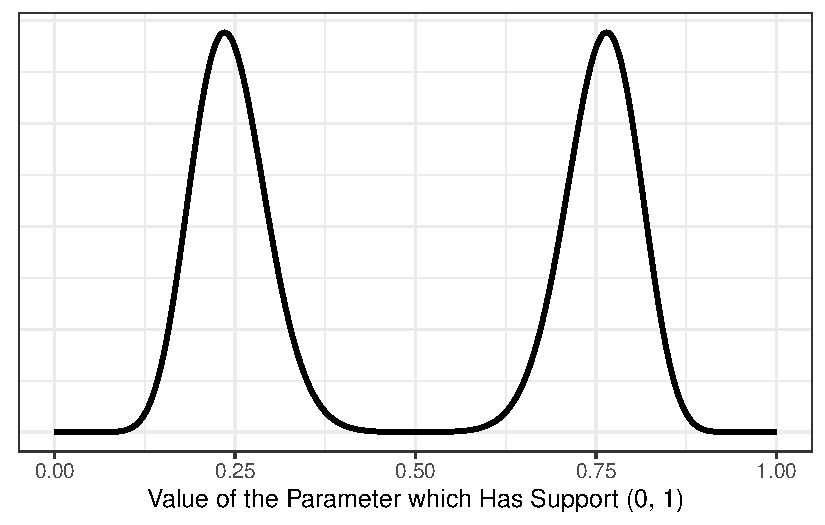
\includegraphics[width=0.8\textwidth,height=\textheight]{./images/fig-mixture-prior-1.pdf}

}

\caption{\label{fig-mixture-prior}Illustration of a mixture prior for a
parameter on the interval (0, 1).}

\end{figure}

\begin{definition}[General Mixture
Distribution]\protect\hypertarget{def-general-mixture-distribution}{}\label{def-general-mixture-distribution}

Let \(\theta\) be a parameter with support \(\Theta\), and let
\(\pi_k(\theta)\) be a valid distribution on the support, for
\(k = 1, 2, \dotsc, K\). Then,

\[\pi(\theta) = \sum_{k=1}^{K} w_k \pi_k(\theta)\]

is a valid prior distribution provided \(\sum_{k=1}^{K} w_k = 1\).

\end{definition}

It turns out that if each component of the mixture distribution
\(\pi_k(\theta)\) is a member of the conjugate family, the entire prior
will be conjugate (a weighted average of distributions). This was
illustrated in Example~\ref{exm-csec-hypotheses}.

Nothing requires that the individual components of a mixture
distribution be of the same family. For example, we might choose to mix
a Normal distribution with a t-distribution in order to capture the
presence of some outliers.

\begin{tcolorbox}[enhanced jigsaw, leftrule=.75mm, coltitle=black, left=2mm, title=\textcolor{quarto-callout-note-color}{\faInfo}\hspace{0.5em}{Note}, breakable, toptitle=1mm, bottomtitle=1mm, colback=white, colbacktitle=quarto-callout-note-color!10!white, titlerule=0mm, opacitybacktitle=0.6, colframe=quarto-callout-note-color-frame, bottomrule=.15mm, arc=.35mm, opacityback=0, rightrule=.15mm, toprule=.15mm]

While we have described the use of a mixture distribution for the prior
distribution, nothing prevents the use from using a mixture distribution
for the likelihood.

\end{tcolorbox}

It has been shown that any distribution can be approximated by some
mixture distribution. That is, if we choose \(K\) to be large enough, we
can approximate any distributional shape with a mixture distribution.

\hypertarget{chains}{%
\section{Chains}\label{chains}}

Within this unit, we have developed the fundamental concepts of Bayesian
inference in a general setting. We have avoided a litany of examples and
instead opted to illustrate the concepts with a single unifying example
throughout the text (Example~\ref{exm-csec}). In both this example and
the exposition in the text, we have acted as though there is a single
parameter \(\theta\) governing the likelihood. Many interesting
questions, however, involve models for the data that depend upon
multiple parameters. These types of problems often necessitate the need
for numerical solutions, which we address in the next unit. Here, we
simply discuss a common tool for constructing priors over multiple
parameters.

When \(\theta\) is a parameter \emph{vector}, then \(\pi(\theta)\) is
actually a \emph{joint} density across all parameters. Therefore, one
key decision that must be made is whether, a priori, we believe these
parameters to be independent of one another.

\begin{example}[Heights of
Children]\protect\hypertarget{exm-heights}{}\label{exm-heights}

During early development, children are regularly benchmarked against
national growth charts. One such chart traces a child's height as they
grow. However, these charts were developed using the entire population
of ``healthy'' children. Suppose I am interested in developing a growth
chart for children with Hispanic parents, as I believe they tend to be a
bit shorter, on average. It is typical to model heights using a Normal
distribution, which has two unknown parameters (which govern the
location and spread of the distribution).

We consider developing a likelihood and prior for this process.

\end{example}

The likelihood for the above example is readily available if we are
willing to assume a random sample of \(n\) children (of the same age)
born to Hispanic parents:

\[
\begin{aligned}
  f(\mathbf{y} \mid \mu, \tau) 
    &= \prod_{i=1}^{n} \frac{\tau^{1/2}}{\sqrt{2\pi}} e^{-\tau/2 (y_i - \mu)^2} \\
    &= \frac{\tau^{n/2}}{(2\pi)^{n/2}} e^{-(\tau/2)\sum_{i=1}^{n}(y_i - \mu)^2}
\end{aligned}
\]

where we have defined the likelihood in terms of the mean \(\mu\) and
the \emph{precision} \(\tau\), which is the inverse of the variance. The
likelihood was simplified by assuming the height of one child is
independent of the height of any other child. Suppose we are further
willing to believe the \emph{parameters} are independent of one another;
then, it is reasonable to propose the prior distributions independently.
Choosing a Normal prior for \(\mu\) and a Gamma prior for \(\tau\), we
could then propose

\[
\begin{aligned}
  \pi(\mu) &= \frac{\sqrt{b}}{\sqrt{2\pi}} e^{-b/2 (\mu - a)^2} \\
  \pi(\tau) &= \frac{s^r}{\Gamma(r)} \tau^{r - 1} e^{-s\tau} \\
  \Rightarrow \pi(\mu, \tau) &= \pi(\mu) \pi(\tau).
\end{aligned}
\]

The joint prior across the parameters is easy to specify because of the
independence assumption. Of course, nothing requires we assume the
parameters are independent of one another; this was a modeling
assumption. A different set of beliefs would lead to a different
structure for the prior. For example, the prior given by

\[
\begin{aligned}
  \pi(\tau) &= \frac{s^2}{\Gamma(r)} \tau^{r - 1} e^{-s\tau} \\
  \pi(\mu \mid \tau) &= \frac{\sqrt{\tau}}{\sqrt{2\pi}} e^{-\tau/2 (\mu - a)^2} \\
  \Rightarrow \pi(\mu, \tau) &= \pi(\mu \mid \tau) \pi(\tau)
\end{aligned}
\]

suggests a Gamma prior for \(\tau\) and a Normal prior for \(\mu\)
\emph{conditional} on the value of \(\tau\). This hierarchical structure
allows the mean \(\mu\) to depend on the precision \(\tau\). The joint
distribution of the parameters (prior to seeing the data) is then the
product of the marginal distribution of \(\tau\) and the conditional
distribution of \(\mu \mid \tau\).

This process of defining a prior in stages, each stage conditioning on
parameters for which a prior distribution is specified, is known as
``chaining.''

Regardless of whether we form a prior through assuming independence or
through chaining, the prior predictive distribution (the denominator in
Bayes Theorem) will have the form

\[\int \int f(\mathbf{y} \mid \mu, \tau) \pi(\mu, \tau) d\mu d\tau.\]

The more parameters we have, the more complex the integration in the
denominator; this is what motivates the computational methods we examine
in the next unit.

\hypertarget{non-informative-priors}{%
\section{Non-Informative Priors}\label{non-informative-priors}}

Each of the above sections assumes that we have prior information that
needs to be encoded into a distribution; we now consider the case when
we have very little (or no) prior information. In such a setting, we
must determine how we encode ``ignorance.''

\begin{definition}[Laplace
Prior]\protect\hypertarget{def-laplace-prior}{}\label{def-laplace-prior}

The Laplace prior, also known as a ``flat'' prior, considers the form

\[\pi(\theta) = 1 \qquad \forall \theta \in \Theta.\]

\end{definition}

\begin{tcolorbox}[enhanced jigsaw, leftrule=.75mm, coltitle=black, left=2mm, title=\textcolor{quarto-callout-warning-color}{\faExclamationTriangle}\hspace{0.5em}{Warning}, breakable, toptitle=1mm, bottomtitle=1mm, colback=white, colbacktitle=quarto-callout-warning-color!10!white, titlerule=0mm, opacitybacktitle=0.6, colframe=quarto-callout-warning-color-frame, bottomrule=.15mm, arc=.35mm, opacityback=0, rightrule=.15mm, toprule=.15mm]

For any unbounded support \(\Theta\), the Laplace prior will be
\emph{improper}; that is,

\[\int \pi(\theta) d\theta = \infty.\]

In such settings the Laplace prior is not actually a valid density
function. This seems like it is breaking all the rules, and to some
degree it is, but it is still commonly used.

\end{tcolorbox}

\begin{tcolorbox}[enhanced jigsaw, leftrule=.75mm, coltitle=black, left=2mm, title=\textcolor{quarto-callout-warning-color}{\faExclamationTriangle}\hspace{0.5em}{Warning}, breakable, toptitle=1mm, bottomtitle=1mm, colback=white, colbacktitle=quarto-callout-warning-color!10!white, titlerule=0mm, opacitybacktitle=0.6, colframe=quarto-callout-warning-color-frame, bottomrule=.15mm, arc=.35mm, opacityback=0, rightrule=.15mm, toprule=.15mm]

The Bayes Factor should never be computed when you have an improper
prior as the prior odds are not defined since there is no valid
probability of each hypothesis a priori.

\end{tcolorbox}

The Laplace prior is a common default prior when no (or little) prior
information is available. However, a flat prior cannot represent total
ignorance. When the parameter space is unbounded, notice that a flat
prior essentially says that no matter how large of a value \(q\) you
imagine, \(Pr\left(\theta > q\right) = \infty\) --- that is, there is
always infinite probability that \(\theta\) is larger than you can
imagine.

\begin{tcolorbox}[enhanced jigsaw, leftrule=.75mm, coltitle=black, left=2mm, title=\textcolor{quarto-callout-tip-color}{\faLightbulb}\hspace{0.5em}{Big Idea}, breakable, toptitle=1mm, bottomtitle=1mm, colback=white, colbacktitle=quarto-callout-tip-color!10!white, titlerule=0mm, opacitybacktitle=0.6, colframe=quarto-callout-tip-color-frame, bottomrule=.15mm, arc=.35mm, opacityback=0, rightrule=.15mm, toprule=.15mm]

Flat priors are chosen because they are easily overwhelmed by the
observed data.

\end{tcolorbox}

The benefit of a flat prior is that the posterior distribution is
proportional to the likelihood. The idea here is to make the Bayesian
framework dependent solely on the data, similar to a Frequentist
approach (though the two are still not guaranteed to give the same
results).

Flat priors are a subset of a larger class of priors that continues to
be an active area of research; this larger class of priors is determined
solely by the form of the likelihood.

\begin{definition}[Noninformative
Prior]\protect\hypertarget{def-noninformative-prior}{}\label{def-noninformative-prior}

A prior distribution which is derived solely based on the form of the
likelihood.

\end{definition}

A noninformative prior seems like a compromise between Bayesians and
those who dislike the subjective nature of a prior distribution. So, why
is this not the standard? On the one hand, true Bayesians argue that we
should make use of prior information; we should not seek to make use of
only the data available in that single study. This allows the
information from one study to become the prior information for a
follow-up study instead of beginning from scratch. Second, there is a
potential pitfall when using noninformative priors when they are
improper --- it is possible for the posterior distribution to be
improper (which is a nice way of saying it is not a distribution at
all)! If the posterior distribution is improper, it cannot yield any
valid inference on the parameters.

\begin{tcolorbox}[enhanced jigsaw, leftrule=.75mm, coltitle=black, left=2mm, title=\textcolor{quarto-callout-warning-color}{\faExclamationTriangle}\hspace{0.5em}{Warning}, breakable, toptitle=1mm, bottomtitle=1mm, colback=white, colbacktitle=quarto-callout-warning-color!10!white, titlerule=0mm, opacitybacktitle=0.6, colframe=quarto-callout-warning-color-frame, bottomrule=.15mm, arc=.35mm, opacityback=0, rightrule=.15mm, toprule=.15mm]

Valid inference cannot be made when the posterior distribution is
improper.

\end{tcolorbox}

An improper prior \emph{can} lead to an improper posterior; however, a
proper prior will \emph{always} lead to a proper posterior. The danger
is that software which automates Bayesian analyses currently have no way
of checking if a posterior is proper; so, this must be done manually. As
computing the posterior can be difficult (the entire reason for the next
unit), this often involves bounding the integral in some way --- a job
for true mathematicians.

Fear around improper priors often leads to what are known as vague
priors. This is taking a parametric family and choosing the
hyperparameters to result in a massive variance so that the prior
distribution, while proper, appears flat over the parameter space. The
idea here is to allow the data to easily overwhelm any prior
information.

\begin{tcolorbox}[enhanced jigsaw, leftrule=.75mm, coltitle=black, left=2mm, title=\textcolor{quarto-callout-tip-color}{\faLightbulb}\hspace{0.5em}{Big Idea}, breakable, toptitle=1mm, bottomtitle=1mm, colback=white, colbacktitle=quarto-callout-tip-color!10!white, titlerule=0mm, opacitybacktitle=0.6, colframe=quarto-callout-tip-color-frame, bottomrule=.15mm, arc=.35mm, opacityback=0, rightrule=.15mm, toprule=.15mm]

Noninformative priors try to make it easy for the likelihood to dominate
the prior distribution in the computation of the posterior distribution.

\end{tcolorbox}

\part{Unit IV: Numerical Approaches to Bayesian Computations}

\providecommand{\norm}[1]{\lVert#1\rVert}
\providecommand{\abs}[1]{\lvert#1\rvert}
\providecommand{\iid}{\stackrel{\text{IID}}{\sim}}
\providecommand{\ind}{\stackrel{\text{Ind}}{\sim}}

\providecommand{\bm}[1]{\mathbf{#1}}
\providecommand{\bs}[1]{\boldsymbol{#1}}
\providecommand{\bbeta}{\bs{\beta}}

\providecommand{\Ell}{\mathcal{L}}
\providecommand{\indep}{\perp\negthickspace\negmedspace\perp}

The previous unit discussed the fundamental components of the Bayesian
paradigm. We began by specifying the likelihood, a model describing the
data generating process as a function of unknown parameters, and a prior
distribution, which captures our beliefs about the unknown parameters
prior to observing data. Using Bayes Theorem, we were able to
characterize our beliefs about the unknown parameter after observing the
data in the posterior distribution. We know that the posterior
distribution is proportional to the product of the likelihood and the
prior; that is,

\[\pi(\boldsymbol{\theta} \mid \mathbf{x}) \propto f(\mathbf{x} \mid \boldsymbol{\theta}) \pi(\boldsymbol{\theta}).\]

However, to determine the exact form of the posterior distribution, we
need to determine the scaling constant given by

\[\frac{1}{\int f(\mathbf{x} \mid \boldsymbol{\theta}) \pi(\boldsymbol{\theta}) d\boldsymbol{\theta}}.\]

Unfortunately, this integral can be intractable, especially as the
dimension of \(\boldsymbol{\theta}\) grows. In this unit, we consider
numerical approaches for common Bayesian quantities, such as point and
interval estimation. With these techniques, we can address more
intricate problems.

\hypertarget{sec-mc-integration}{%
\chapter{Monte Carlo Integration}\label{sec-mc-integration}}

\providecommand{\norm}[1]{\lVert#1\rVert}
\providecommand{\abs}[1]{\lvert#1\rvert}
\providecommand{\iid}{\stackrel{\text{IID}}{\sim}}
\providecommand{\ind}{\stackrel{\text{Ind}}{\sim}}

\providecommand{\bm}[1]{\mathbf{#1}}
\providecommand{\bs}[1]{\boldsymbol{#1}}
\providecommand{\bbeta}{\bs{\beta}}

\providecommand{\Ell}{\mathcal{L}}
\providecommand{\indep}{\perp\negthickspace\negmedspace\perp}

Integration plays an integral part (pun completely intended) in Bayesian
inference. Integration is necessary to determine the scaling term for
the posterior distribution; it is necessary to perform point and
interval estimation; it is necessary for computing posterior
probabilities needed for hypotheses testing; integration is at center of
all Bayesian computations. The integrals we need to compute are also
typically analytically intractable. This chapter introduces a numerical
integration technique popular within the statistical community that
serves as the foundation for modern Bayesian computational approaches we
will consider in the remainder of this unit.

Example~\ref{exm-integration} illustrates the need for numerical
integration techniques in practice.

\begin{example}[Pharmacokinetics]\protect\hypertarget{exm-integration}{}\label{exm-integration}

When modeling the rate at which a drug is broken down by the body (known
as pharmacokinetics), it is often of interest to know the logarithm of
the ED50 value (the time at which 50\% of the drug has been metabolized
by the body). Suppose it is known that for a particular drug, the ED50
value \(T\) for the patient population can be modeled using a Gamma
distribution with a shape parameter \(a = 4\) and a rate parameter of
\(b = 2\). That is, the density of \(T\) is given by

\[f(t) = \frac{b^a}{\Gamma(a)} t^{a-1} e^{-bt}\]

on the interval \(t > 0\), where \(a = 4\) and \(b = 2\). We are
interested in the average logarithm of the ED50 value, which is given by

\[\int \log(t) f(t) dt.\]

\end{example}

While this example is contrived (the parameters governing the
distribution of the ED50 value are known explicitly), integrals like
this arise in practice regularly. The integral of interest does not
yield an analytical solution; a numerical procedure must be used. While
there are several numerical methods for integration which are developed
and studied in mathematics, many are restricted to low dimensional
problems. We need a technique which is applicable in high dimensions. As
a foundation, consider the following suggested procedure:

\begin{itemize}
\tightlist
\item
  Let \(T_1, T_2, \dots, T_n\) be a random sample such that
  \(T_i \sim f(t)\) for all \(i\).
\item
  Define \(Y_i = \log\left(T_i\right)\) for all \(i\).
\item
  Compute \(\bar{Y}\).
\end{itemize}

The value of \(\bar{Y}\) will estimate the integral! As an initial
justification, observe that on average, the estimate is correct. That
is, consider taking the expected value of \(\bar{Y}\); specifically,

\begin{equation}\protect\hypertarget{eq-mc-step1}{}{
\begin{aligned}
  E\left(\bar{Y}\right) &= E\left(n^{-1} \sum_{i=1}^{n} Y_i\right) \\
    &= E\left(n^{-1} \sum_{i=1}^{n} \log\left(T_i\right)\right) \\
    &= n^{-1} \sum_{i=1}^{n} E\left(\log\left(T_i\right)\right), \\
\end{aligned}
}\label{eq-mc-step1}\end{equation}

where the last line is a result of the expectation being a linear
operator. Since each \(T_i\) is identically distributed (we have a
random sample from the population), the expectation is the same for each
\(i\); specifically, we have (see Definition~\ref{def-expectation})

\[E\left(\log\left(T_i\right)\right) = \int \log(t) f(t) dt.\]

Since the right-hand side is not indexed by \(i\), substituting back
into Equation~\ref{eq-mc-step1}, we have that

\[E\left(\bar{Y}\right) = \int \log(t) f(t) dt.\]

That is, the expected value of \(\bar{Y}\) is the desired integral. Of
course, this just states that the distribution of \(\bar{Y}\) (across
many samples of size \(n\)) will center on the true value of the
integral; it does not guarantee the average we compute for any specific
\(n\) will be accurate. However, the Law of Large numbers gives a
stronger result.

\hypertarget{law-of-large-numbers}{%
\section{Law of Large Numbers}\label{law-of-large-numbers}}

Let \(X_1, X_2,\dotsc, X_n\) be independent and identically distributed
random variables with density \(f(x)\). Consider a real valued function
\(g\). Then, for any \(\epsilon > 0\) we have that

\[Pr\left(\lvert\frac{1}{n}\sum_{i=1}^n g\left(X_i\right) - E\left[g(X)\right]\rvert > \epsilon\right) \rightarrow 0\]

as \(n \rightarrow \infty\), assuming \(E\left[g(X)\right]\) exists.

The Law of Large Numbers essentially says that the sample mean can be
made arbitrarily close to the expectation it approximates given a large
enough sample size. That is, as the sample size increases, the sample
mean is really close to the true mean. Using mathematical notation, this
means

\[\frac{1}{n} \sum_{i=1}^{n} g\left(X_i\right) \approx \int g(x) f(x) dx.\]

\begin{tcolorbox}[enhanced jigsaw, leftrule=.75mm, coltitle=black, left=2mm, title=\textcolor{quarto-callout-tip-color}{\faLightbulb}\hspace{0.5em}{Big Idea}, breakable, toptitle=1mm, bottomtitle=1mm, colback=white, colbacktitle=quarto-callout-tip-color!10!white, titlerule=0mm, opacitybacktitle=0.6, colframe=quarto-callout-tip-color-frame, bottomrule=.15mm, arc=.35mm, opacityback=0, rightrule=.15mm, toprule=.15mm]

The Law of Large Numbers allows us to approximate integrals, in the form
of expectations of random variables, using a corresponding sample mean.

\end{tcolorbox}

In practice, limited resources (namely, time and money) limit the size
of the sample we can consider in our study, which in turn limits the
applicability of the Law of Large Numbers. However, numerical
integration makes use of a computational study (all the ``data'' is
generated within the computer), where speed and cost are greatly
reduced. Therefore, the Law of Large Numbers is more applicable to such
computational studies.

The following pseudo-code illustrates the use of the Law of Large
Numbers in order to compute the integral that corresponds to the average
logarithm of the ED50 value in Example~\ref{exm-integration}:

\begin{verbatim}
let m = 10000;

for i from 1 to m do;
  x[i] = random_gamma(shape = 4, rate = 2);
  y[i] = log(x[i]);
end;
  
ybar = mean(y[1:m]);
\end{verbatim}

Since we have a large sample size, we know that the sample mean computed
in the last step will be a good approximation to the integral of
interest.

Upon first inspection, it may seem that the Law of Large Numbers is
limited to estimating means. However, nearly every quantity of interest
can be written in terms of an integral and therefore approximated using
this technique. This includes probabilities, means, quantiles (and
therefore credible intervals), variances, and even the evidence in favor
of a model. That is, the Law of Large Numbers provides a technique for
performing integration numerically, allowing us to compute summaries for
the posterior distribution. Because of its dependence on random
processes, this integration technique is known as Monte Carlo (or MC)
Integration.

\begin{definition}[Monte Carlo
Integration]\protect\hypertarget{def-mc-integration}{}\label{def-mc-integration}

Consider an integral of the form

\[\int_{\mathcal{S}} g(x) f(x) dx\]

where \(f(x)\) is a valid density function for a random variable \(X\)
with support \(\mathcal{S}\). Then, the following algorithm, known as
Monte Carlo (or MC) Integration, gives a numerical approximation to the
integral:

\begin{enumerate}
\def\labelenumi{\arabic{enumi}.}
\tightlist
\item
  Take a random sample \(X_1, X_2, \dotsc, X_m\) such that
  \(X_i \sim f(x)\) for all \(i\), where \(m\) is large.
\item
  Compute \(m^{-1} \sum_{i=1}^{m} g\left(X_i\right)\).
\end{enumerate}

By the Law of Large Numbers,

\[\frac{1}{m} \sum_{i=1}^{m} g\left(X_i\right) \approx \int_{\mathcal{S}} g(x) f(x) dx.\]

\end{definition}

\begin{tcolorbox}[enhanced jigsaw, leftrule=.75mm, coltitle=black, left=2mm, title=\textcolor{quarto-callout-tip-color}{\faLightbulb}\hspace{0.5em}{Big Idea}, breakable, toptitle=1mm, bottomtitle=1mm, colback=white, colbacktitle=quarto-callout-tip-color!10!white, titlerule=0mm, opacitybacktitle=0.6, colframe=quarto-callout-tip-color-frame, bottomrule=.15mm, arc=.35mm, opacityback=0, rightrule=.15mm, toprule=.15mm]

We can construct Bayesian estimators using only a random sample from the
posterior distribution.

\end{tcolorbox}

\begin{example}[Estimating a Posterior
Probability]\protect\hypertarget{exm-probability-integration}{}\label{exm-probability-integration}

Assume that our beliefs about an unknown parameter \(\theta\) (with
support on the real line), given an observed sample \(\mathbf{x}\), is
characterized by the posterior distribution
\(\pi(\theta \mid \mathbf{x})\). Derive a Monte Carlo Integration
technique for estimating the probability

\[Pr(\theta > q \mid \mathbf{x}) = \int_{q}^{\infty} \pi(\theta \mid \mathbf{x}) d\theta.\]

\end{example}

\begin{solution}

First, we recognize that the probability of interest is naturally an
integral. As currently written, however, the integral is not over the
entire support of \(\theta\). Note, however, that we can rewrite the
integral to be over the entire support. Specifically, observe that

\[
\begin{aligned}
  Pr(\theta > q \mid \mathbf{x})
    &= \int_{q}^{\infty} \pi(\theta \mid \mathbf{x}) d\theta \\
    &= \int_{-\infty}^{q} 0 \cdot \pi(\theta \mid \mathbf{x}) d\theta + \int_{q}^{\infty} 1 \cdot \pi(\theta \mid \mathbf{x}) d\theta \\
    &= \int_{-\infty}^{\infty} \mathbb{I}(\theta > q) \pi(\theta \mid \mathbf{x}) d\theta,
\end{aligned}
\]

where \(\mathbb{I}(u)\) is the ``indicator function'' taking the value 1
if \(u\) occurs and 0 otherwise. Specifically, in this case

\[\mathbb{I}(q < \theta) = \begin{cases} 1 & \text{if } \theta > q \\ 0 & \text{if } \theta \leq q. \end{cases}\]

Having rewritten the integral of interest, we now recognize that

\[Pr(\theta > q \mid \mathbf{x}) = E\left[\mathbb{I}(\theta > q) \mid \mathbf{x}\right].\]

That is, the posterior probability of interest is the posterior mean of
the quantity \(\mathbb{I}(\theta > q)\).

Applying the Law of Large Numbers, our MC Integration technique is
defined by the following algorithm:

\begin{enumerate}
\def\labelenumi{\arabic{enumi}.}
\tightlist
\item
  Take a random sample \(\theta^*_1, \theta^*_2, \dotsc, \theta^*_m\)
  from the posterior distribution,
  \(\theta^*_i \sim \pi(\theta \mid \mathbf{x})\) for all \(i\) where
  \(m\) is large.
\item
  Compute
  \(m^{-1} \sum_{i=1}^{m} \mathbb{I}\left(\theta^*_i > q\right)\).
\end{enumerate}

This sample mean (which essentially computes the proportion of the
\(\theta^*\) values which exceed \(q\)) approximates the integral of
interest. Further, according to the Law of Large Numbers, \(m\) can be
chosen to make the approximation as precise as desired.

\end{solution}

In practice, there are multiple unknown parameters; therefore, the
posterior distribution is a \emph{joint density}. As a result, when
applying MC Integration in practice, we must often generate random
variates from a joint distribution. In general, such generation is
difficult to perform directly; however, the process is much simpler if
we can create a set of chained expressions to guide the generation.
Suppose \((X, Y)\) is a vector of two random variables with joint
density \(f(x, y)\); recall that

\[f(x, y) = f(x \mid y) f(y);\]

that is, the joint distribution is the product of a conditional
distribution and a marginal distribution. This suggests a procedure for
generating from a joint distribution.

\begin{tcolorbox}[enhanced jigsaw, leftrule=.75mm, coltitle=black, left=2mm, title=\textcolor{quarto-callout-tip-color}{\faLightbulb}\hspace{0.5em}{Simulating from a Joint Distribution}, breakable, toptitle=1mm, bottomtitle=1mm, colback=white, colbacktitle=quarto-callout-tip-color!10!white, titlerule=0mm, opacitybacktitle=0.6, colframe=quarto-callout-tip-color-frame, bottomrule=.15mm, arc=.35mm, opacityback=0, rightrule=.15mm, toprule=.15mm]

Let the random vector \((X, Y)\) be distributed according to the joint
density \(f(x,y)\). The following procedure can be used to simulate
observations
\(\left(X_1, Y_1\right), \left(X_2, Y_2\right), \dotsc, \left(X_m, Y_m\right)\)
from the joint density:

\begin{enumerate}
\def\labelenumi{\arabic{enumi}.}
\tightlist
\item
  Generate \(m\) variates \(Y_1, Y_2, \dotsc, Y_m\) from \(f(y)\), the
  marginal distribution of \(Y\).
\item
  For each \(Y_i\), generate a single \(X_i\) from \(f(x \mid y)\), the
  conditional distribution of \(X\) given \(Y\).
\end{enumerate}

The resulting pairs will have the desired joint distribution. Further,
the column of \(X\)'s will behave according to the density \(f(x)\), the
marginal distribution of \(X\).

\end{tcolorbox}

The Law of Large Numbers guarantees that we can obtain approximations of
Bayesian estimators; further, it guarantees these approximations can be
made arbitrarily good by choosing a large enough sample size \(m\). Of
course, in practice we will specify the value of \(m\); and, since MC
Integration relies on random processes, it is reasonable to ask how good
the resulting approximation is. Similarly, it is natural to ask how many
random samples are needed for an approximation with a specific amount of
precision. This is addressed via a version of the Central Limit Theorem.

\begin{theorem}[Central Limit
Theorem]\protect\hypertarget{thm-clt}{}\label{thm-clt}

Let \(X_1, X_2, \dotsc, X_m\) be independent and identically distributed
random variables. Consider a real-valued function \(g\) such that
\(E\left[g(X)\right]\) and \(Var\left[g(X)\right]\) exist. Then, we have
that the quantity

\[\frac{\sqrt{m} \left[m^{-1} \sum_{i=1}^{m} g\left(X_i\right) - E\left[g(X)\right]\right]}{\sqrt{\widehat{Var}\left[g(X)\right]}}\]

behaves like a standard normal random variable as
\(m \rightarrow \infty\).

\end{theorem}

The Central Limit Theorem provides a way of quantifying the error in the
Monte Carlo approximation.

\begin{definition}[Monte Carlo
Error]\protect\hypertarget{def-mc-error}{}\label{def-mc-error}

Also called the standard error for an approximation of the form
\(m^{-1} \sum\limits_{k=1}^{m} g\left(X_k\right)\), the MC error is
given by

\[\sqrt{\frac{1}{m(m-1)} \sum_{k=1}^{m} \left[g\left(X_k\right) - \frac{1}{m} \sum_{j=1}^{m} g\left(X_j\right)\right]^2}\]

which is the sample standard deviation of the generated variates divided
by the square root of the number of replications.

\end{definition}

We close this chapter by revisiting
Example~\ref{exm-csec-point-estimate}; instead of an analytical
solution, we apply the techniques discussed in this chapter to provide a
numeric solution to estimating the unknown parameter.

\begin{example}[C-section Deliveries
Continued]\protect\hypertarget{exm-csec-mc-integration}{}\label{exm-csec-mc-integration}

Example~\ref{exm-csec} introduced a study, a component of which includes
estimating the probability of a mother undergoing a C-section delivery
at a particular hospital.

Example~\ref{exm-csec-posterior} found the posterior distribution to be

\[\theta \mid \mathbf{x} \sim Beta\left(n + a, n\bar{x} + b\right)\]

where \(a = 17, b = 39, n = 15\) and \(n\bar{x} = 33\) given the
observed data.\\
Example~\ref{exm-csec-point-estimate} showed that the posterior mean,
estimating the rate of C-sections at the hospital given the observed
data, is given by 0.308. First, use MC Integration to compute this
estimate, and then estimate the \emph{odds} of a C-section at the
hospital given the observed data.

\end{example}

\begin{solution}

The posterior mean is given by

\[E\left(\theta \mid \mathbf{x}\right) = \int \theta \pi(\theta \mid \mathbf{x}) d\theta.\]

Now, as seen in Example~\ref{exm-csec-point-estimate}, there is a
closed-form expression for this quantity. However, here, we rely on MC
Integration technique. The following pseudo-code illustrates the
process:

\begin{verbatim}
let m = 10000;

for i from 1 to m do;
  x[i] = random_beta(shape1 = (15 + 17), shape2 = (33 + 39));
end;
  
xbar = mean(x[1:m]);
\end{verbatim}

The quantity \texttt{xbar} is an estimate of the posterior mean. This
code requires we have access to a function \texttt{random\_beta()} which
generates a (pseudo) random variate from a Beta distribution with
specified shape parameters. Given a function
\texttt{standard\_deviation()} which computes the sample standard
deviation of a vector of values, we can compute the MC error in the
approximation with

\begin{verbatim}
MCerrorx = sqrt(standard_deviation(x[1:m]) / m);
\end{verbatim}

One implementation of this algorithm gave an estimate of 0.308 with an
MC error of 0.0021. While this computation simply illustrated the
process, the next is computation greatly simplifies our burden of work.

We now consider estimating the odds of a C-section at this hospital,
given the data. The odds of an event with rate \(\theta\) are defined as
\(\theta / (1 - \theta)\). Appealing to
Definition~\ref{def-expectation}, the posterior mean of the odds is then

\[E\left[\frac{\theta}{1 - \theta} \mid \mathbf{x}\right] = \int \frac{\theta}{1-\theta} \pi(\theta \mid \mathbf{x}) d\theta.\]

A closed-form solution for this integral is not readily available;
however, a slight modification of our previous pseudo-code allows us to
numerically compute this integral:

\begin{verbatim}
let m = 10000;

for i from 1 to m do;
  x[i] = random_beta(shape1 = (15 + 17), shape2 = (33 + 39));
  y[i] = x[i] / (1 - x[i]);
end;
  
ybar = mean(y[1:m]);
MCerrory = sqrt(standard_deviation(y[1:m] / m));
\end{verbatim}

The quantity \texttt{ybar} is an estimate of the posterior mean for the
odds of interest. One implementation of this algorithm gave an estimate
of 0.451 with an MC error of 0.0031.

\end{solution}

\begin{tcolorbox}[enhanced jigsaw, leftrule=.75mm, coltitle=black, left=2mm, title=\textcolor{quarto-callout-tip-color}{\faLightbulb}\hspace{0.5em}{Big Idea}, breakable, toptitle=1mm, bottomtitle=1mm, colback=white, colbacktitle=quarto-callout-tip-color!10!white, titlerule=0mm, opacitybacktitle=0.6, colframe=quarto-callout-tip-color-frame, bottomrule=.15mm, arc=.35mm, opacityback=0, rightrule=.15mm, toprule=.15mm]

Given a large random sample from the posterior distribution, we
approximate posterior quantities of interest using the corresponding
sample statistic.

\end{tcolorbox}

\hypertarget{sec-mcmc}{%
\chapter{Markov Chain Monte Carlo (MCMC)}\label{sec-mcmc}}

\providecommand{\norm}[1]{\lVert#1\rVert}
\providecommand{\abs}[1]{\lvert#1\rvert}
\providecommand{\iid}{\stackrel{\text{IID}}{\sim}}
\providecommand{\ind}{\stackrel{\text{Ind}}{\sim}}

\providecommand{\bm}[1]{\mathbf{#1}}
\providecommand{\bs}[1]{\boldsymbol{#1}}
\providecommand{\bbeta}{\bs{\beta}}

\providecommand{\Ell}{\mathcal{L}}
\providecommand{\indep}{\perp\negthickspace\negmedspace\perp}

The previous chapter laid the foundation for Bayesian computations:
given a random sample from the posterior distribution, we can
approximate any Bayesian estimator, and the level of approximation is
only limited by the size of the sample we can take. When the posterior
distribution has the form of a known distribution, there are often
built-in functions for obtaining a (pseudo) random sample. The majority
of applications, however, involve posterior distributions which cannot
be derived analytically. In such cases, Markov Chain Monte Carlo (MCMC)
techniques are used to sample from the posterior distribution. Once we
have a sample from the posterior distribution, we apply the MC
Integration techniques from the previous chapter for computing
estimates. In this chapter, we give a brief overview of MCMC techniques.

The technical details of MCMC can be overwhelming; we begin by
discussing the conceptual goal of the algorithm, and we do that through
Example~\ref{exm-mcmc-concepts}.

\begin{example}[Relative Wealth (MCMC
Concepts)]\protect\hypertarget{exm-mcmc-concepts}{}\label{exm-mcmc-concepts}

Suppose you are attending a large gathering of your relatives. Given
your current status as a student (without no income), you would like to
network with these relatives in hopes that they will write you into
their will, ensuring you a sizable inheritance. Naturally, you would
like to be strategic about how much time you spend with each person,
dividing your time with each person proportionally according to their
wealth (spend more time with wealthier individuals). However, you face a
couple of problems.

\begin{itemize}
\tightlist
\item
  Problem 1: you are uncertain about how many people are actually
  attending the party.\\
\item
  Problem 2: you have no way of determining the wealth of each person.
\end{itemize}

However, while no one is willing to share their actual wealth, each
person is willing to share a bit of information with you. If you show
interest in speaking with them, the individual will let you know their
wealth relative to that of the person you are currently speaking with
(``I am half as rich as the person you are speaking with,'' for
example).

We want an algorithm for determining who to speak with, and for how long
to speak with them.

\end{example}

While Example~\ref{exm-mcmc-concepts} is a toy problem, it illustrates
the obstacles we are trying to overcome with MCMC methods. We want to
take a sample from the posterior distribution, but we do not have the
form of the posterior distribution. Instead, we only know the kernel:

\[\pi(\theta \mid \mathbf{y}) \propto f(\mathbf{y} \mid \theta) \pi(\theta).\]

The first ``problem'' in Example~\ref{exm-mcmc-concepts} reflects our
uncertainty about where we should focus our attention within the
posterior. We have a sense of the support of the posterior, but there
may be large areas of the posterior which have essentially probability 0
of occurring. The second ``problem'' is that we do not have the value of
the posterior; instead, we are only able to compute the posterior up to
some scalar constant. Therefore, while we are not able to compute the
value of the posterior, we can accurately determine the ratio of the
posterior between two points. Observe that

\[\pi(\theta \mid \mathbf{y}) = \frac{f(\mathbf{y} \mid \theta) \pi(\theta)}{m(\mathbf{y})},\]

where \(m(\mathbf{y})\) represents the prior predictive distribution
(see Definition~\ref{def-prior-predictive-distribution}). Now, we have
that the ratio of the posterior evaluated at \(\theta = a\), relative to
the posterior evaluated at \(\theta = b\) is given by

\[
\begin{aligned}
  \frac{\pi(\theta = a \mid \mathbf{y})}{\pi(\theta = b \mid \mathbf{y})} 
    &= \frac{(1/m(\mathbf{y})) f(\mathbf{y} \mid \theta = a) \pi(\theta = a)}{(1/m(\mathbf{y})) f(\mathbf{y} \mid \theta = b)\pi(\theta b)} \\
    &= \frac{f(\mathbf{y} \mid \theta = a) \pi(\theta = a)}{f(\mathbf{y} \mid \theta = b)\pi(\theta = b)}.
\end{aligned}
\]

That is, the ratio of the posterior evaluated at two points can be
determined using only the kernel of the distribution. We now consider an
algorithm for talking to your relatives that addresses
Example~\ref{exm-mcmc-concepts}.

\begin{solution}

Consider the following scheme. You randomly choose a person to begin
speaking with (your ``partner''). After a fixed period of time, you will
flip a coin. If the coin is ``heads up,'' you will consider speaking
with the person to your partner's right; if the coin is ``tails up,''
you will consider speaking with the person to your partner's left. This
determines your ``candidate.''

You ask the candidate about their wealth relative to your current
partner. If your candidate is wealthier than your partner, you will
definitely move to them and make them your new partner. If your
candidate is less wealthy than your partner, however, you will only move
to them with a probability equivalent to the candidate's wealth relative
to your current partner's. That is, if the candidate is half as wealthy
as your current partner, you will move to the candidate with probability
0.5.

You then repeat this process many times.

\end{solution}

This process summarizes the idea behind MCMC methods. We generate a
candidate value of the parameter; if the value of the posterior at the
candidate value is higher than our current position, then we choose to
move to the candidate point. Otherwise, we move to the candidate point
with a probability equal to the ratio of the posterior for the candidate
relative to our current position. We move through the parameter space in
this fashion until we have generated a large sample from the posterior
(say 3000 replicates).

The above thought exercise illustrates one of the simplest algorithms
for generating from an unknown density, known as the Metropolis
Algorithm. While in practice this algorithm is rarely implemented
directly, it forms the basis of several more complex algorithms, and it
illustrates the basic properties of all MCMC methods.

\begin{definition}[Metropolis
Algorithm]\protect\hypertarget{def-metropolis-algorithm}{}\label{def-metropolis-algorithm}

Suppose we want to generate random variates from the density
\(\pi(\theta \mid \mathbf{y})\). We perform the following steps:

\begin{enumerate}
\def\labelenumi{\arabic{enumi}.}
\tightlist
\item
  Generate an initial value \(\theta^{(0)}\).\\
\item
  At the \(k\)-th step, generate \(\theta^*\) (a candidate) according to
  a symmetric proposal density
  \(q\left(\theta \mid \theta^{(k-1)}\right)\).\\
\item
  Compute \(A\left(\theta^*, \theta^{(k-1)}\right)\) where
  \[A\left(\theta^*, \theta^{(k-1)}\right) = \frac{\pi\left(\theta^* \mid \mathbf{y}\right)}{\pi\left(\theta^{(k-1)} \mid \mathbf{y}\right)} = \frac{f\left(\mathbf{y} \mid \theta^*\right) \pi\left(\theta^*\right)}{f\left(\mathbf{y} \mid \theta^{(k-1)}\right) \pi\left(\theta^{(k-1)}\right)}.\]
\item
  Generate \(U \sim Unif(0,1)\). If
  \(U \leq A\left(\theta^*, \theta^{(k-1)}\right)\), then set
  \(\theta^{(k)} = \theta^*\); else, set
  \(\theta^{(k)} = \theta^{(k-1)}\).
\item
  Repeat Steps 2-4 \(m\) times, for some large \(m\).
\end{enumerate}

When generating an initial value, \(\theta^{(0)}\), we could choose
\(\theta^{(0)} \sim \pi(\theta)\) if the prior is easy to generate from.
While it is common to choose \(q(\cdot)\) to be a Normal distribution
with mean \(\theta^{(k-1)}\), it is not a requirement to do so; when a
Normal distribution is used, it can be difficult to determine a
reasonable variance (too large, and you drift too far away; too small,
and you do not move at all).

\end{definition}

The Metropolis Algorithm is typically run several thousand times,
resulting in what is known as a Markov Chain.

\begin{definition}[Markov
Chain]\protect\hypertarget{def-markov-chain}{}\label{def-markov-chain}

A sequence of random vectors
\(\theta^{(0)}, \theta^{(1)}, \theta^{(2)}, \dotsc, \theta^{(n)}\) is a
Markov Chain with stationary transition probabilities if for any set
\(A\) and any \(k \leq n\)

\[
\begin{aligned}
  Pr\left(\theta^{(k)} \in A \mid \theta^{(1)}, \theta^{(2)}, \dotsc, \theta^{(k-1)}\right)
    &= Pr\left(\theta^{(k)} \in A \mid \theta^{(k-1)}\right) \\
    &= \int_{A} q\left(\theta^{(k)} \mid \theta^{(k-1)}\right) d\theta^{(k)}
\end{aligned}
\]

where \(q\) is called the transition kernel.

\end{definition}

In general, Markov chains are not required to have stationary transition
probabilities, but it is a nice simplifying assumption that is applied
in Bayesian computing methods. Markov chains are a topic of interest in
and of themselves in probability theory and are beyond the scope of this
text. We primarily focus on the fact that the probability that a value
is in some region depends \emph{only} on the previous state; the
remaining ``history'' (previous states in the chain) is unimportant.

The Markov Chain is essentially a sample; of course, for it to be
useful, we need to establish that the chain is also representative of
the appropriate target distribution. That is, we need to know the Markov
Chain represents the posterior distribution. This target distribution
has a name in Markov Chain literature --- the ``stationary
distribution.''

\begin{definition}[Stationary
Distribution]\protect\hypertarget{def-stationary-distribution}{}\label{def-stationary-distribution}

Let \(\theta^{(0)}, \theta^{(1)}, \theta^{(2)}, \dotsc, \theta^{(n)}\)
be a Markov Chain. The stationary distribution of the Markov Chain is
the distribution \(p(\theta)\) such that

\[Pr\left(\theta^{(k)} \in A\right) = \int_{A} p(\theta) d\theta.\]

\end{definition}

The stationary distribution is where the Markov Chain settles down so
that the probability that any variate is in some region is computed
using that same distribution \(p\) (as opposed to the transition
kernel). You can think of it as the limit of the transition kernel as
\(k\) gets large.

The idea is to choose a proposal density \(q\) in the Metropolis
Algorithm such that the stationary distribution of the resulting Markov
Chain, if one exists, will be the posterior distribution of interest.
So, we want to pick a proposal density \(q\) that is easy to generate
from, is symmetric, and so that eventually, the values we are generating
behave as if they were drawn from the posterior distribution. The
machinery needed to prove such results is beyond the scope of our text,
but it can be shown that the Metropolis Algorithm produces a Markov
Chain for which the stationary distribution is the same as the posterior
distribution, provided that the proposal density is symmetric. That is,
as \(k\) increases, the values generated by this algorithm behave as if
they were drawn from the posterior distribution. More, we can show that
this is true regardless of the choice of the starting value
\(\theta^{(0)}\).

\begin{tcolorbox}[enhanced jigsaw, leftrule=.75mm, coltitle=black, left=2mm, title=\textcolor{quarto-callout-note-color}{\faInfo}\hspace{0.5em}{Note}, breakable, toptitle=1mm, bottomtitle=1mm, colback=white, colbacktitle=quarto-callout-note-color!10!white, titlerule=0mm, opacitybacktitle=0.6, colframe=quarto-callout-note-color-frame, bottomrule=.15mm, arc=.35mm, opacityback=0, rightrule=.15mm, toprule=.15mm]

It can be shown that the the Metropolis Algorithm has the posterior
distribution as the stationary distribution of the Markov Chain, but the
Metropolis Algorithm is not always the most efficient algorithm for
generating from the posterior distribution. In practice, other
algorithms, such as the Gibbs sampler or Hamiltonian Monte Carlo,
improve on the efficiency by implementing modifications to the above
Metropolis Algorithm.

\end{tcolorbox}

We now have a way of generating values which have properties similar to
random variates drawn from the posterior distribution. The language here
is chosen with care because, as always, there is a catch: \textbf{the
values generated in the Markov Chain are identically distributed, but
are not independent.}

In practice, analysts often state that they have obtained a random
sample from the posterior using MCMC methods; and, we can often proceed
as if that were true. However, when we use MCMC methods, the resulting
sample is not truly a ``random sample'' in the sense of being IID. The
points are identically distributed, but since each variate in the sample
was generated based on the value of the previous variate, there is a
dependence between the variates. Fortunately, this dependence between
values generated consecutively (known as autocorrelation) is often
negligible in practice.

The real issue is that the theory introduced in
Chapter~\ref{sec-mc-integration} relied on having a random sample (IID
variates). Therefore, the fact that the Markov Chain generated by the
Metropolis Algorithm does not result in independent observations seems
to imply that we are unable to rely on MC Integration. Fortunately,
however, there is a Law of Large Numbers-type result for Markov Chains
which says

\[\lim\limits_{m \rightarrow \infty} \frac{1}{m} \sum_{k=1}^{m} g\left(\theta^{(k)}\right) = \int g(\theta) p(\theta) d\theta\]

where \(g(\cdot)\) is some real-valued function and \(p(\theta)\) is the
stationary distribution of the Markov Chain, if it exists. This result
says that even though the points are related, as we take a large number
of them, we can approximate integrals (therefore, Bayesian estimators)
using sample averages. That is, we can apply MC Integration techniques
to Markov Chains.

\begin{tcolorbox}[enhanced jigsaw, leftrule=.75mm, coltitle=black, left=2mm, title=\textcolor{quarto-callout-tip-color}{\faLightbulb}\hspace{0.5em}{Big Idea}, breakable, toptitle=1mm, bottomtitle=1mm, colback=white, colbacktitle=quarto-callout-tip-color!10!white, titlerule=0mm, opacitybacktitle=0.6, colframe=quarto-callout-tip-color-frame, bottomrule=.15mm, arc=.35mm, opacityback=0, rightrule=.15mm, toprule=.15mm]

For a sufficiently large number of replications, the Markov Chain
resulting from an MCMC algorithm will behave as a random sample from the
posterior distribution.

\end{tcolorbox}

\hypertarget{hamiltonian-monte-carlo}{%
\section{Hamiltonian Monte Carlo}\label{hamiltonian-monte-carlo}}

The trick to MCMC methods is to choose a transition kernel that is
efficient and can handle the myriad of situations encountered in
practice. The Metropolis Algorithm, while simplistic, is not very
efficient, and can be quite difficult to implement when the dimension of
the parameter vector increases. A commonly implemented alternative is
known as the Gibbs sampler. This is implemented in the popular Bayesian
software packages
\href{https://www.mrc-bsu.cam.ac.uk/software/bugs/}{BUGS} (Bayesian
inference Using Gibbs Sampling) and
\href{https://mcmc-jags.sourceforge.io/}{JAGS} (Just Another Gibbs
Sampler). BUGS is a standalone software package while JAGS is
implemented in other computing languages (like R and Python). These
software packages provide a myriad of algorithms based on the Gibbs
sampler which address hierarchical models in a nice way. However, in
some complex models, these algorithms can be inefficient or fail to
produce variates from the posterior. \href{https://mc-stan.org/}{Stan}
implements a Hamiltonian Monte Carlo (HMC) algorithm which can succeed
in these situations. While the details of the algorithm are beyond the
scope of this text, we discuss the ways in which HMC improves upon the
Metropolis Algorithm discussed above.

The Metropolis Algorithm can be summarized in the following two
statements:

\begin{itemize}
\tightlist
\item
  Choose the candidate point using a symmetric proposal distribution
  centered on the current point.
\item
  Favor points with a larger corresponding posterior density, moving to
  candidate points with lower posterior density probabilistically.
\end{itemize}

The key distinction between the Metropolis Algorithm and HMC is to allow
the proposal distribution to be dependent upon our current location.

\begin{tcolorbox}[enhanced jigsaw, leftrule=.75mm, coltitle=black, left=2mm, title=\textcolor{quarto-callout-tip-color}{\faLightbulb}\hspace{0.5em}{Big Idea}, breakable, toptitle=1mm, bottomtitle=1mm, colback=white, colbacktitle=quarto-callout-tip-color!10!white, titlerule=0mm, opacitybacktitle=0.6, colframe=quarto-callout-tip-color-frame, bottomrule=.15mm, arc=.35mm, opacityback=0, rightrule=.15mm, toprule=.15mm]

HMC uses proposal distributions which favor moving toward the posterior
mode.

\end{tcolorbox}

The idea is illustrated in Figure~\ref{fig-mcmc-p1}, created by John
Kruschke (Kruschke 2015), which shows how proposals are generated for
two different initial values. Note, the end result in this graphic is
not a sample from the posterior but the distribution of potential next
steps.

\begin{figure}

{\centering 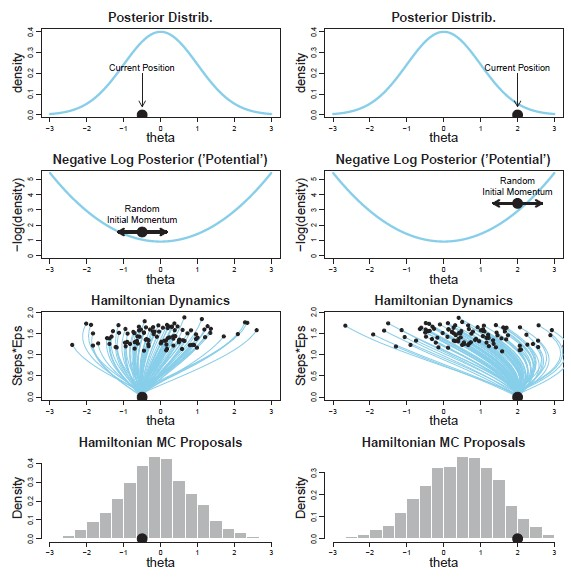
\includegraphics{images/Kruschke-Fig1.jpg}

}

\caption{\label{fig-mcmc-p1}Examples of Hamiltonian Monte Carlo proposal
distributions. Two columns show two different current parameter values,
marked by a large dot. The first row shows the posterior distribution.
The second row shows the potential energy, with a random impulse given
to the dot. The third row shows trajectories, which are the theta value
(x-axis) as a function of time (y-axis marked Steps*Eps). The fourth row
shows histograms of the proposals.}

\end{figure}

To illustrate how this works, consider two different current positions
within a posterior distribution. The Metropolis Algorithm would simply
say to generate proposals which are symmetric about the current
position. HMC generates proposals that are closer to the posterior mode
(as evidenced by the bottom part of the figure where the majority of
proposals are near the mode). In order to determine where to move from
the current position, the HMC algorithm considers the \emph{potential}
of the position, defined through the negative log-density. The potential
gives an idea of how far we might want to travel (the potential of the
position to change).

\begin{definition}[Potential]\protect\hypertarget{def-potential}{}\label{def-potential}

The potential of a value \(\theta\) is the negative logarithm of the
posterior evaluated at \(\theta\). In practice, we need only know the
potential up to a constant. That is, it suffices to define the potential
as

\[\text{Potential}(\theta) = -\log\left[f(\mathbf{y} \mid \theta) \pi(\theta)\right].\]

\end{definition}

While we have described the potential as a value, since it exists for
all \(\theta\) in the support, we can think of the potential as a
function (row 2 of Figure~\ref{fig-mcmc-p1}). Now, imagine the current
position is a ball on the potential; the proposed position is determined
by flicking the ball randomly. This random ``flick'' is done by
selecting a random variable from a Standard Normal distribution, which
determines both the magnitude and direction of the flick (negative
values move the ball to the left, and positive values move the ball to
the right). We then watch the ball roll around for a while. Wherever the
ball stops is the proposed position. This is illustrated in the third
row of graphics in Figure~\ref{fig-mcmc-p1} that show how the ball moves
over time to the proposed position.

\begin{tcolorbox}[enhanced jigsaw, leftrule=.75mm, coltitle=black, left=2mm, title=\textcolor{quarto-callout-note-color}{\faInfo}\hspace{0.5em}{Note}, breakable, toptitle=1mm, bottomtitle=1mm, colback=white, colbacktitle=quarto-callout-note-color!10!white, titlerule=0mm, opacitybacktitle=0.6, colframe=quarto-callout-note-color-frame, bottomrule=.15mm, arc=.35mm, opacityback=0, rightrule=.15mm, toprule=.15mm]

The sum of potential and kinetic energy is known as the Hamiltonian
(hence the name of this procedure). The total energy should be conserved
at each point in the algorithm.

\end{tcolorbox}

As the ball rolls around on the potential, it will naturally be drawn to
lower points on this surface. That is, candidate points will tend to be
drawn from regions with lower potential, corresponding to regions with a
higher posterior density. Notice that when the current position is near
the posterior mode, the potential positions are nearly symmetric about
the current location as in the Metropolis Algorithm. But, if the current
position is far from the posterior mode, the potential positions are
drawn from regions closer to the posterior mode and the potential
positions are far from the current position.

\begin{tcolorbox}[enhanced jigsaw, leftrule=.75mm, coltitle=black, left=2mm, title=\textcolor{quarto-callout-tip-color}{\faLightbulb}\hspace{0.5em}{Big Idea}, breakable, toptitle=1mm, bottomtitle=1mm, colback=white, colbacktitle=quarto-callout-tip-color!10!white, titlerule=0mm, opacitybacktitle=0.6, colframe=quarto-callout-tip-color-frame, bottomrule=.15mm, arc=.35mm, opacityback=0, rightrule=.15mm, toprule=.15mm]

The HMC algorithm generates proposals which tend to have lower
potential.

\end{tcolorbox}

We emphasize that these are just \emph{candidate} positions. Once a
candidate position is identified, we must decide whether to move there
or remain in the current position, just as we do in the Metropolis
Algorithm.

\begin{tcolorbox}[enhanced jigsaw, leftrule=.75mm, coltitle=black, left=2mm, title=\textcolor{quarto-callout-important-color}{\faExclamation}\hspace{0.5em}{Decision Rule for HMC:}, breakable, toptitle=1mm, bottomtitle=1mm, colback=white, colbacktitle=quarto-callout-important-color!10!white, titlerule=0mm, opacitybacktitle=0.6, colframe=quarto-callout-important-color-frame, bottomrule=.15mm, arc=.35mm, opacityback=0, rightrule=.15mm, toprule=.15mm]

Generate \(U \sim Unif(0,1)\) and
\(A\left(\theta^*, \theta^{(k-1)}\right)\) where

\[A\left(\theta^*, \theta^{(k-1)}\right) = \frac{f\left(\mathbf{y} \mid \theta^*\right) \pi\left(\theta^*\right) \omega\left(\theta^*\right)}{f\left(\mathbf{y} \mid \theta^{(k-1)}\right) \pi\left(\theta^{(k-1)}\right) \omega\left(\theta^{(k-1)}\right)}\]

and \(\omega(\cdot)\) is the momentum. If
\(U \leq A\left(\theta^*, \theta^{(k-1)}\right)\), then we move to the
new position; otherwise, we remain in the same position.

\end{tcolorbox}

The momentum can be thought of as how much speed the ball has when you
reach the candidate position (remember, we stop the ball not when it
comes to rest but after some fixed amount of time). Recall that we apply
a random momentum to the current location of the ball. The aspect we
want to emphasize here is that the decision rule is quite similar to the
Metropolis Algorithm.

We have described this process as letting the ``ball roll around'' for
some fixed set of time. In practice, we emulate this by taking some
predefined number of steps of a certain size based on the gradient (much
like numeric function minimization). Both the step size and number of
steps require some tuning. The step size is tuned to balance how far
away from the current position we move and the degree of approximation.
If we take small steps, we approximate the curve quite nicely, but we do
not get anywhere. If we take large steps, we move away from our current
position, but the approximation suffers. The total duration (the number
of steps taken) is tuned to ensure we do not overshoot or make a u-turn.
If we let the ball roll for too long, it could overshoot the posterior
mode by a large degree; or, we may end up stopping the ball when it has
rolled back to where it started. Figure~\ref{fig-mcmc-p2}, created by
John Kruschke (Kruschke 2015), illustrates the impact of allowing the
``time'' (number of steps and length of step size) to be too large;
notice the difference in the distribution of candidate points in
Figure~\ref{fig-mcmc-p2} compared to Figure~\ref{fig-mcmc-p1}.

\begin{figure}

{\centering 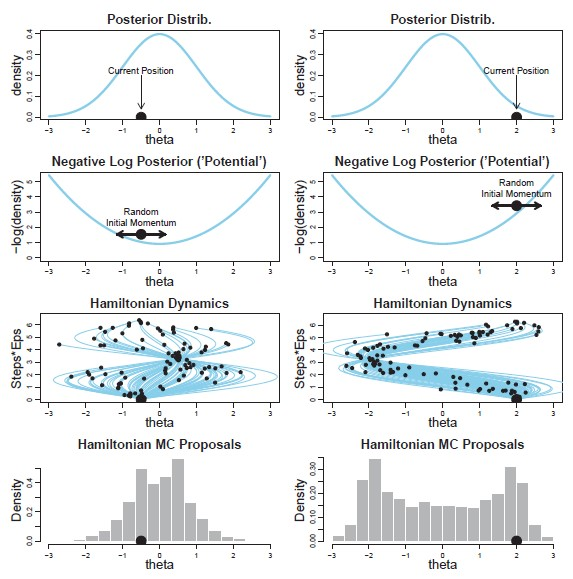
\includegraphics{images/Kruschke-Fig2.jpg}

}

\caption{\label{fig-mcmc-p2}Examples of Hamiltonian Monte Carlo proposal
distributions for two different current parameter values, marked by the
large dots, in the two columns. For this figure, a large range of random
trajectory lengths (Steps*Eps) is sampled.}

\end{figure}

In addition to these tuning parameters, we must determine the standard
deviation of the symmetric distribution used to apply the momentum to
the current position. This choice needs to balance variety with
accuracy. Too small of a standard deviation (like nudging the ball)
means it will not roll far from where it started, and every candidate is
essentially the same (leading to a higher likelihood of
acceptance/rejection). Too large of a standard deviation, and a high
degree of candidates will be rejected. Figure~\ref{fig-mcmc-p3}, created
by John Kruschke (Kruschke 2015), illustrates the impact of standard
deviation in the proposal distribution; notice the difference in the
distribution of candidate points between the two columns in
Figure~\ref{fig-mcmc-p3}.

\begin{figure}

{\centering 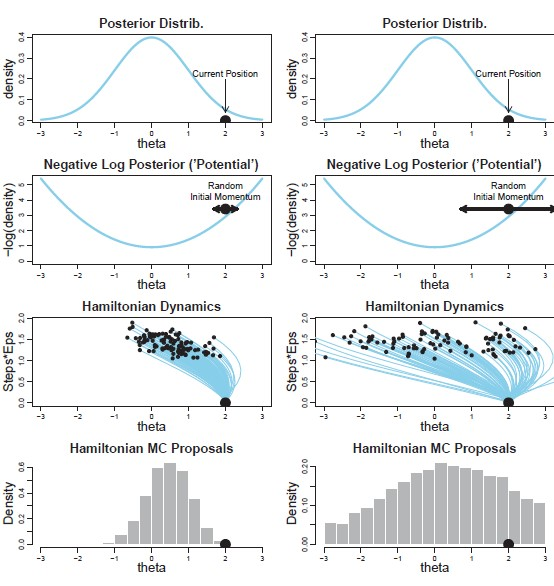
\includegraphics{images/Kruschke-Fig3.jpg}

}

\caption{\label{fig-mcmc-p3}Examples of a Hamiltonian Monte Carlo
proposal distributions for two different variances of the initial random
momentum, indicated in the second row.}

\end{figure}

Proper tuning ensures that the algorithm is efficient and a majority of
the variates are useful in representing the posterior. These are handled
internally by the software, but it is important to have an understanding
of what is happening in the background.

With MCMC methods, we can address a multitude of more complex problems.
We do note the one limitation of Stan is that it does not currently
support discrete parameters directly. This is because the HMC algorithm
needs a smooth function in order to compute the gradient. Not supporting
discrete parameters is not as limiting as it might seem, but it does
prohibit automatic model comparison within Stan and eliminates the
ability to put a point mass in the prior distribution.

\begin{tcolorbox}[enhanced jigsaw, leftrule=.75mm, coltitle=black, left=2mm, title=\textcolor{quarto-callout-warning-color}{\faExclamationTriangle}\hspace{0.5em}{Warning}, breakable, toptitle=1mm, bottomtitle=1mm, colback=white, colbacktitle=quarto-callout-warning-color!10!white, titlerule=0mm, opacitybacktitle=0.6, colframe=quarto-callout-warning-color-frame, bottomrule=.15mm, arc=.35mm, opacityback=0, rightrule=.15mm, toprule=.15mm]

While you could write custom implementations of the HMC (or any MCMC)
algorithm, software like Stan does the hard work for you. However, in
order to make use of those tools, you must specify the Bayesian model
(the likelihood and the prior) in addition to providing the data. This
can require your learning a new ``probability language'' (as opposed to
a computing language) for specifying such models. Some software packages
have pre-built functions/interfaces for commonly specified models
allowing you to get started more quickly.

\end{tcolorbox}

\hypertarget{sec-mcmc-assessment}{%
\chapter{Assessing MCMC Samples}\label{sec-mcmc-assessment}}

\providecommand{\norm}[1]{\lVert#1\rVert}
\providecommand{\abs}[1]{\lvert#1\rvert}
\providecommand{\iid}{\stackrel{\text{IID}}{\sim}}
\providecommand{\ind}{\stackrel{\text{Ind}}{\sim}}

\providecommand{\bm}[1]{\mathbf{#1}}
\providecommand{\bs}[1]{\boldsymbol{#1}}
\providecommand{\bbeta}{\bs{\beta}}

\providecommand{\Ell}{\mathcal{L}}
\providecommand{\indep}{\perp\negthickspace\negmedspace\perp}

The reliability of any statistical analysis depends on the quality of
the data obtained; as a result, any good analysis requires that we give
some thought to the data we have obtained. Similarly, we must consider
the derivation of our prior distribution and the reasonableness of our
model for the likelihood. When our analysis also includes the use of an
MCMC algorithm, we should, at a minimum, also investigate that certain
assumptions about the resulting sample are reasonable before proceeding.
This chapter briefly discusses some checks that are done on the
posterior sample to determine its suitability for answering questions.

There are essentially four considerations when examining the output of
any MCMC algorithm.

\begin{tcolorbox}[enhanced jigsaw, leftrule=.75mm, coltitle=black, left=2mm, title=\textcolor{quarto-callout-important-color}{\faExclamation}\hspace{0.5em}{Assessment of an MCMC Algorithm}, breakable, toptitle=1mm, bottomtitle=1mm, colback=white, colbacktitle=quarto-callout-important-color!10!white, titlerule=0mm, opacitybacktitle=0.6, colframe=quarto-callout-important-color-frame, bottomrule=.15mm, arc=.35mm, opacityback=0, rightrule=.15mm, toprule=.15mm]

Before using a sample from an MCMC algorithm, the following should be
considered:

\begin{enumerate}
\def\labelenumi{\arabic{enumi}.}
\tightlist
\item
  The posterior distribution is proper.
\item
  The resulting Markov Chains converged.
\item
  Sensitivity of the algorithm to starting values.
\item
  The correlation between generated variates is negligible.
\end{enumerate}

\end{tcolorbox}

Software which implements MCMC algorithms typically generate output for
assessing the reliability of the resulting sample. In this chapter, we
focus on navigating this output for assessment.

An improper posterior distribution cannot provide valid inference.
Unfortunately, an MCMC algorithm will generate a sequence of values,
even if the target distribution is improper. If the combination of the
likelihood and prior specified would result in an improper posterior,
the resulting sample from the MCMC algorithm is useless. In general,
software is unable to determine if the target distribution is improper;
therefore, it is up to the analyst to analytically determine if the
posterior distribution is proper. The simplest way to ensure that we
have a proper posterior distribution is to use a proper prior
distribution.

\begin{tcolorbox}[enhanced jigsaw, leftrule=.75mm, coltitle=black, left=2mm, title=\textcolor{quarto-callout-note-color}{\faInfo}\hspace{0.5em}{Ensuring a Proper Posterior}, breakable, toptitle=1mm, bottomtitle=1mm, colback=white, colbacktitle=quarto-callout-note-color!10!white, titlerule=0mm, opacitybacktitle=0.6, colframe=quarto-callout-note-color-frame, bottomrule=.15mm, arc=.35mm, opacityback=0, rightrule=.15mm, toprule=.15mm]

If we use a proper prior, we are guaranteed a proper posterior.

\end{tcolorbox}

\begin{example}[C-section Deliveries
Continued]\protect\hypertarget{exm-csec-check1}{}\label{exm-csec-check1}

Example~\ref{exm-csec} introduced a study, a component of which includes
estimating the probability of a mother undergoing a C-section delivery
at a particular hospital.

While MCMC methods are not required for this example, as
Example~\ref{exm-csec-posterior} illustrates, it is possible to use and
MCMC algorithm to address this question. Before even writing MCMC code,
explain why we can be confident that the posterior is proper in this
case.

\end{example}

\begin{solution}

Our prior information was represented using a Beta distribution, which
is a proper distribution. Therefore, we know the posterior will also be
proper.

\end{solution}

Recall that we ``seed'' an MCMC algorithm with an initial value. Only
after a large number of iterations is the algorithm generated values
from the stationary distribution --- the distribution to which the
process essentially converges. Therefore, we must ensure we have allowed
the algorithm to run long enough that the process has converged to the
stationary distribution --- that the variates generate behave as if they
are drawn from the posterior distribution. A \emph{trace plot} showing
the value of the generated variates at each step of the algorithm can be
used to visually assess convergence.

You are essentially looking for whether the chain eventually settles in
a particular region of the parameter space; this should not be confused
with the chain reaching a specific value. As we are looking for a
stationary distribution, we expect the variates generated to bounce
around (according to the stationary distribution); however, if the chain
has some signal to it (trending in location or spread), that is
unexpected. It should eventually look like noise around some central
point.

Often, we eliminate the early part of a chain, the discarded portion
known as the ``warm-up'' (or ``burn-in'') period. That is, we might
remove the first 1000 variates from the resulting Markov chain because
we expect the chain is still moving toward the stationary distribution
during this time period. The variates after the burn-in period behave
more like a sample from the stationary distribution and are retained for
analysis.

\begin{tcolorbox}[enhanced jigsaw, leftrule=.75mm, coltitle=black, left=2mm, title=\textcolor{quarto-callout-note-color}{\faInfo}\hspace{0.5em}{Graphically Assessing Convergence of MCMC Chains}, breakable, toptitle=1mm, bottomtitle=1mm, colback=white, colbacktitle=quarto-callout-note-color!10!white, titlerule=0mm, opacitybacktitle=0.6, colframe=quarto-callout-note-color-frame, bottomrule=.15mm, arc=.35mm, opacityback=0, rightrule=.15mm, toprule=.15mm]

Create a plot of the values generated (after eliminated the values from
the burn-in period) against the order in which they were generated. This
is known as a ``trace plot.'' If the chain has converged, the plot
should not have any trends in the location or spread over time.

\end{tcolorbox}

\begin{example}[C-section Deliveries
Continued]\protect\hypertarget{exm-csec-check2}{}\label{exm-csec-check2}

Example~\ref{exm-csec} introduced a study, a component of which includes
estimating the probability of a mother undergoing a C-section delivery
at a particular hospital.

We used Stan to implement a Hamiltonian Monte Carlo to obtain a sample
from the posterior distribution. We generated three chains (each seeded
with a different initial value); each chain had 5000 iterations, with
the first 2000 representing a burn-in. This provided a sample of size
9000 from the posterior distribution after combining the three chains.

Table~\ref{tbl-csec-mcmc} summarizes the sample generated by the MCMC
algorithm. Figure~\ref{fig-csec-traceplot} is a trace plot for each of
the three chains. Comment on the convergence of each chain.

\end{example}

\hypertarget{tbl-csec-mcmc}{}
\begin{table}
\caption{\label{tbl-csec-mcmc}Summary of results from MCMC algorithm used to estimate the rate of
C-sections at a hospital. The model was fit with Stan; 3 chains were
generated, each with 5000 iterations and a burn-in of 2000 for a total
of 9000 post-burn-in variates. The 95\% credible interval reported is an
equal-tailed interval. }\tabularnewline

\centering
\begin{tabular}[t]{rrrrr}
\toprule
Posterior Mean & Posterior Median & 95\% Credible Interval & ESS & Shrink Ratio\\
\midrule
\cellcolor{gray!6}{0.307} & \cellcolor{gray!6}{0.306} & \cellcolor{gray!6}{(0.224, 0.397)} & \cellcolor{gray!6}{3495.544} & \cellcolor{gray!6}{1.001}\\
\bottomrule
\end{tabular}
\end{table}

\begin{figure}

{\centering 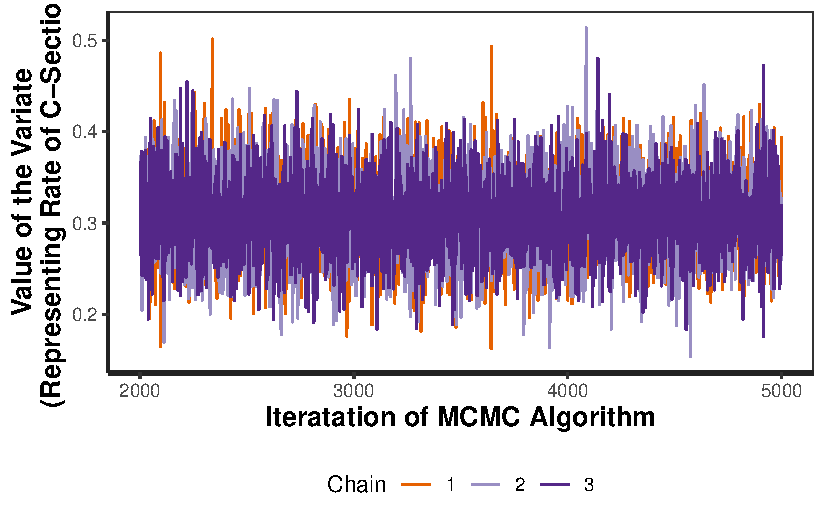
\includegraphics[width=0.8\textwidth,height=\textheight]{./images/fig-csec-traceplot-1.pdf}

}

\caption{\label{fig-csec-traceplot}Traceplot from an example estimating
the rate of C-sections at a hospital. The burn-in of 2000 iterates is
removed from the graphic.}

\end{figure}

\begin{solution}

We do not notice any trends in the location or spread of any of the
three chains after the burn-in period. Each of the chains seems to
bounce around the value 0.3, and the spread stays relatively constant
(values generated tend to be between 0.2 and 0.4).

As there are no trends in the location or spread, the samples generated
by the algorithm are consistent with what we would expect if they had
reached the stationary distribution.

\end{solution}

In theory, the stationary distribution is the posterior distribution, we
just need to run the algorithm long enough to get there. Practically,
however, the distribution to which the algorithm converges could depend
on the value used to seed the process. If that happens, then any results
based on the sample are potentially biased. Therefore, we want to
determine if the MCMC algorithm is sensitive to the chosen starting
(initial) value. To do so, we seed the algorithm with multiple starting
values, resulting in multiple chains. It is generally sufficient to
consider three chains. Overlaying the trace plot from each chain allows
us to assess whether the chains ``mix'' well. If the various chains are
distinct, this suggests that the stationary distribution suggested by
the algorithm varies according to the starting value, which means a
stationary distribution was not really obtained.

In addition to the visual check, we can compute the ``shrink factor.''
Also known as the ``potential scale reduction factor,'' this is the
ratio of the between-chain variability to the within-chain variability.
If the chains are well mixed, this ratio should be near 1. If the ratio
gets much larger than 1.1, it indicates a serious problem with the
mixing.

\begin{tcolorbox}[enhanced jigsaw, leftrule=.75mm, coltitle=black, left=2mm, title=\textcolor{quarto-callout-note-color}{\faInfo}\hspace{0.5em}{Assessing Sensitivity of MCMC Algorithm to Starting Value}, breakable, toptitle=1mm, bottomtitle=1mm, colback=white, colbacktitle=quarto-callout-note-color!10!white, titlerule=0mm, opacitybacktitle=0.6, colframe=quarto-callout-note-color-frame, bottomrule=.15mm, arc=.35mm, opacityback=0, rightrule=.15mm, toprule=.15mm]

Seed the algorithm with three initial values. If the trace plots of the
resulting chains are distinct --- occupy different aspects of the
parameter space --- then your results are sensitive to the starting
value. If the chains mix well, the chains are then combined to form a
single sample for estimation.

Alternatively, a shrink factor above 1.1 indicates sensitivity to the
starting value.

\end{tcolorbox}

\begin{example}[C-section Deliveries
Continued]\protect\hypertarget{exm-csec-check3}{}\label{exm-csec-check3}

Example~\ref{exm-csec} introduced a study, a component of which includes
estimating the probability of a mother undergoing a C-section delivery
at a particular hospital.

Revisiting Example~\ref{exm-csec-check2} above, assess the sensitivity
of the algorithm to the initial value.

\end{example}

\begin{solution}

Notice that in Figure~\ref{fig-csec-traceplot}, the three chains overlap
completely; in fact, it is difficult to distinguish one chain from
another. This suggests the chains are mixing well as they occupy the
same part of the parameter space.

Reported in Table~\ref{tbl-csec-mcmc}, the shrink factor was estimated
to be 1, which is consistent with our observations in the graphic above.
There is no evidence the algorithm is sensitive to the initial value,
and it seems reasonable to combine the variates from the three chains.

\end{solution}

Recall that we expect our Markov chain to result in correlated variates.
As a result, each variate does not contain as much unique information as
we may believe. The ``effective sample size'' gives a crude measure of
how much \emph{independent} information there is within the chain. For
example, we may generate 5000 iterates, but if the variates are highly
dependent, the effective sample size may suggest we act as if only 100
iterates were generated.

\begin{definition}[Effective Sample
Size]\protect\hypertarget{def-ess}{}\label{def-ess}

The effective sample size (ESS) is given by

\[ESS = \frac{N}{1 + 2\sum_{k=1}^{\infty} ACF(k)}\]

where ACF is the auto-correlation function of degree \(k\).

\end{definition}

\begin{tcolorbox}[enhanced jigsaw, leftrule=.75mm, coltitle=black, left=2mm, title=\textcolor{quarto-callout-warning-color}{\faExclamationTriangle}\hspace{0.5em}{Warning}, breakable, toptitle=1mm, bottomtitle=1mm, colback=white, colbacktitle=quarto-callout-warning-color!10!white, titlerule=0mm, opacitybacktitle=0.6, colframe=quarto-callout-warning-color-frame, bottomrule=.15mm, arc=.35mm, opacityback=0, rightrule=.15mm, toprule=.15mm]

When discussing MCMC procedures, it is common to use ``sample size'' to
actually refer to the number of variates generated during the MCMC
algorithm. We should not confuse the number of variates generated from
the posterior with the number of observations in our data set.

\end{tcolorbox}

If you want to measure something that is toward the center of the
distribution (mean/median), the ESS need not be large. But, if you want
to compute a tail probability (such as for a credible interval), you
need a much larger ESS. Some texts recommend near 10000 variates from
the posterior in order to reliably compute a highest posterior density
interval, for example.

\begin{tcolorbox}[enhanced jigsaw, leftrule=.75mm, coltitle=black, left=2mm, title=\textcolor{quarto-callout-note-color}{\faInfo}\hspace{0.5em}{Assessing Independence of Variates}, breakable, toptitle=1mm, bottomtitle=1mm, colback=white, colbacktitle=quarto-callout-note-color!10!white, titlerule=0mm, opacitybacktitle=0.6, colframe=quarto-callout-note-color-frame, bottomrule=.15mm, arc=.35mm, opacityback=0, rightrule=.15mm, toprule=.15mm]

The effective sample size (ESS) takes into account the correlation
between the variates and gives you an indication of how precise your
results are. A small ESS suggests high correlation between the variates
and indicates that your results are less reliable.

\end{tcolorbox}

\begin{example}[C-section Deliveries
Continued]\protect\hypertarget{exm-csec-check4}{}\label{exm-csec-check4}

Example~\ref{exm-csec} introduced a study, a component of which includes
estimating the probability of a mother undergoing a C-section delivery
at a particular hospital.

Revisiting Example~\ref{exm-csec-check2}, assess the independence of the
variates.

\end{example}

\begin{solution}

We see that while we generated 9000 (post burn-in) variates, the
effective sample size is estimated to be just under 3500. This suggests
that there is a relatively strong correlation between the observations;
only every third variate generated is independent. However, the
effective sample size still remains fairly large; so, we are confident
in both our point estimates and any credible intervals generated.

\end{solution}

While these four checks are somewhat universal, there is an additional
check that can be helpful when using a Hamiltonian Monte Carlo (HMC)
algorithm. Recall that the total energy should be conserved during the
HMC procedure. A \emph{divergent transition} occurs when the simulated
Hamiltonian departs from the true value (as measured at the initial
point). Divergent transitions (after warm-up) indicate the results will
be biased. A ``pairs plot'' allows us to visualize when this occurs. If
the amount of error (divergence) is larger than the median, it can often
be fixed by increasing the target acceptance rate. If not, then this
indicates that the posterior may be very difficult to sample from for
this algorithm.

\begin{tcolorbox}[enhanced jigsaw, leftrule=.75mm, coltitle=black, left=2mm, title=\textcolor{quarto-callout-note-color}{\faInfo}\hspace{0.5em}{Assessing Divergent Transitions}, breakable, toptitle=1mm, bottomtitle=1mm, colback=white, colbacktitle=quarto-callout-note-color!10!white, titlerule=0mm, opacitybacktitle=0.6, colframe=quarto-callout-note-color-frame, bottomrule=.15mm, arc=.35mm, opacityback=0, rightrule=.15mm, toprule=.15mm]

For the HMC algorithm only, a pairs plot allows us to determine if the
amount of divergence is larger than expected. If there are issues, try
increasing the target acceptance rate.

\end{tcolorbox}

With regard to Example~\ref{exm-csec-check2}, no divergent iterations
were noted among the 9000 variates generated.

Posterior checks of the MCMC samples are necessary in order to prevent
making conclusions that are unreasonable. We have only discussed how to
identify problems. Fixing the problems is often dependent upon the
specific application. There are several subtleties with each model that
take time to learn in order to understand where the algorithm might get
hung-up. The fix is often a clever reparameterization of the likelihood
or prior in order to help the algorithm. With enough computation, we can
overcome many of the problems faced.

\part{Unit V: Hierarchical Models for Comparing Groups}

Unit III introduced the fundamentals of the Bayesian framework. While
the text introduced these ideas in a general setting, the running
example through that unit considered modeling a single response
variable. In this unit, we consider comparing a response across groups.
While the framework remains the same, we discuss additional
considerations to be made in these settings.

\hypertarget{sec-study-design}{%
\chapter{Elements of Good Study Design}\label{sec-study-design}}

\providecommand{\norm}[1]{\lVert#1\rVert}
\providecommand{\abs}[1]{\lvert#1\rvert}
\providecommand{\iid}{\stackrel{\text{IID}}{\sim}}
\providecommand{\ind}{\stackrel{\text{Ind}}{\sim}}

\providecommand{\bm}[1]{\mathbf{#1}}
\providecommand{\bs}[1]{\boldsymbol{#1}}
\providecommand{\bbeta}{\bs{\beta}}

\providecommand{\Ell}{\mathcal{L}}
\providecommand{\indep}{\perp\negthickspace\negmedspace\perp}

Thinking about how the data was collected helps us determine how the
results generalize beyond the sample itself (to what population the
results apply). When our question of interest is about the relationship
between two variables (as most questions are), we must also carefully
consider the study design. Too often separated from the statistical
analysis that follows, keeping the study design in mind should guide the
analysis as well as inform us about the conclusions we can draw.

\hypertarget{two-types-of-studies}{%
\section{Two Types of Studies}\label{two-types-of-studies}}

In order to illustrate how study design can impact the results, consider
the following example.

\begin{example}[Kangaroo
Care]\protect\hypertarget{exm-data-kangaroo}{}\label{exm-data-kangaroo}

At birth, infants have low levels of Vitamin K, a vitamin needed in
order to form blood clots. Though rare, without the ability for her
blood to clot, an infant could develop a serious bleed. In order to
prevent this, the American Academy of Pediatrics recommends that all
infants be given a Vitamin K shot shortly after birth in order to raise
Vitamin K levels. As with any shot, there is typically discomfort to the
infant, which can be very discomforting to new parents.

Kangaroo Care is a method of holding a baby which emphasizes
skin-to-skin contact. The child, who is dressed only in a diaper, is
placed upright on the parent's bare chest; a light blanket is draped
over the child. Suppose we are interested in determining if utilizing
the method while giving the child a Vitamin K shot reduces the
discomfort in the infant, as measured by the total amount of time the
child cries following the shot.

Within this context, contrast the following two potential study designs:

\begin{enumerate}
\def\labelenumi{(\Alph{enumi})}
\tightlist
\item
  We allow the attending nurse to determine whether Kangaroo Care is
  initiated prior to giving the Vitamin K shot. Following the shot, we
  record the total time (in seconds) the child cries.\\
\item
  We flip a coin. If it comes up heads, the nurse should have the
  parents implement Kangaroo Care prior to giving the Vitamin K shot; if
  it comes up tails, the nurse should give the Vitamin K shot without
  implementing Kangaroo Care. Following the shot, we record the total
  time (in seconds) the child cries.
\end{enumerate}

Note, in both study designs (A) and (B), we only consider term births
which have no complications to avoid situations that might alter the
timing of the Vitamin K shot or the ability to implement Kangaroo Care.

\end{example}

Note that there are some similarities in the two study designs:

\begin{itemize}
\tightlist
\item
  The underlying population is the same for both designs: infants born
  at term with no complications.
\item
  There are two groups being compared in both designs: the ``Kangaroo
  Care'' group and the ``no Kangaroo Care'' group.
\item
  The response (variable of interest) is the same in both designs: the
  time (in seconds) the infant cries.
\item
  There is action taken by the researcher in both designs: a Vitamin K
  shot is given to the child.
\end{itemize}

There is one prominent difference between the two study designs:

\begin{itemize}
\tightlist
\item
  For design (A), the choice of Kangaroo Care is left up to the nurse
  (self-selected); for design (B), the choice of Kangaroo is
  \emph{assigned} to the nurse by the researcher, and this selection is
  made \emph{at random}.
\end{itemize}

Design (A) is an example of an \textbf{observational study}; design (B)
is a an example of a \textbf{controlled experiment}.

\begin{definition}[Observational
Study]\protect\hypertarget{def-observational-study}{}\label{def-observational-study}

A study in which each subject ``self-selects'' into one of groups being
compared in the study. The phrase ``self-selects'' is used very loosely
here and can include studies for which the groups are defined by an
inherent characteristic or are chosen haphazardly.

\end{definition}

\begin{definition}[Controlled
Experiment]\protect\hypertarget{def-controlled-experiment}{}\label{def-controlled-experiment}

A study in which each subject is \emph{randomly} assigned to one of the
groups being compared in the study.

\end{definition}

It is common to think that anytime the environment is ``controlled'' by
the researcher that a controlled experiment is taking place, but the
defining characteristic is the random assignment to groups (sometimes
referred to as the \emph{factor} under study or \emph{treatment}
groups). In the example above, both study designs involved a controlled
setting (the delivery room of a hospital) in which trained staff (the
nurse) deliver the shot. However, only design (B) is a controlled
experiment because the researchers randomly determined which treatment
the infant would receive.

To understand the impact of random allocation, suppose that we had
conducted a study using design (A); further, the results of the study
suggest that those infants who were given a shot while using Kangaroo
Care cried for a shorter time period, on average. Can we conclude that
it was the Kangaroo Care that led to the shorter crying time? Maybe.
Consider the following two potential explanations for the resulting
data:

\begin{enumerate}
\def\labelenumi{(\arabic{enumi})}
\tightlist
\item
  Kangaroo Care is very effective; as a result, those children who are
  given Kangaroo Care cry for less time, on average, following the
  Vitamin K shot.\\
\item
  It turns out that those nurses who choose to implement Kangaroo Care
  (remember, they have a choice under design (A) whether they implement
  the method) are also the nurses with a gentler bedside manner.
  Therefore, these nurses tend to be very gentle when giving the Vitamin
  K shot whereas the nurses who choose not to implement Kangaroo Care
  tend to jab the needle when giving the shot. The reduced crying time
  is not a result of the Kangaroo Care but the manner in which the shot
  was given.
\end{enumerate}

The problem is that we are unable to determine which of the explanations
is correct under study design (A). Given the data we have collected, we
are unable to tease out the effect of the Kangaroo Care from that of the
nurse's bedside manner. As a result, we are able to say we observed an
\emph{association} between the use of Kangaroo Care and reduced crying
time, but we are unable to conclude that Kangaroo Care \emph{caused} a
reduction in the crying time (that is, the reduced crying time may be
due to something else, like the bedside manner of the nurse). In this
hypothetical scenario, the nurse's bedside manner is called a
\textbf{confounder}.

\begin{definition}[Confounding]\protect\hypertarget{def-confounding}{}\label{def-confounding}

When the effect of a variable on the response is mis-represented due to
the presence of a third, potentially unobserved, variable known as a
confounder.

\end{definition}

\begin{tcolorbox}[enhanced jigsaw, leftrule=.75mm, coltitle=black, left=2mm, title=\textcolor{quarto-callout-note-color}{\faInfo}\hspace{0.5em}{Note}, breakable, toptitle=1mm, bottomtitle=1mm, colback=white, colbacktitle=quarto-callout-note-color!10!white, titlerule=0mm, opacitybacktitle=0.6, colframe=quarto-callout-note-color-frame, bottomrule=.15mm, arc=.35mm, opacityback=0, rightrule=.15mm, toprule=.15mm]

While both result in estimates we may not trust, confounding is not
equivalent to a biased sample.

\end{tcolorbox}

Confounders can mask the relationship between the factor under study and
the response. Did you know there is a documented association between ice
cream sales and the risk of shark attacks? As ice cream sales increase,
the risk of a shark attack also tends to increase. This does not mean
that if a small city in the Midwest increases its ice cream sales that
the citizens are at higher risk of being attacked by a shark. As
Figure~\ref{fig-data-confounding} illustrates, there is a confounder ---
temperature. As the temperatures increase, people tend to buy more ice
cream; as the temperature increases, people tend to go to the beach,
thereby increasing the risk of a shark attack. The two variables, ice
cream sales and shark attacks, appear to be related as a result of the
confounder of temperature.

\begin{figure}

{\centering 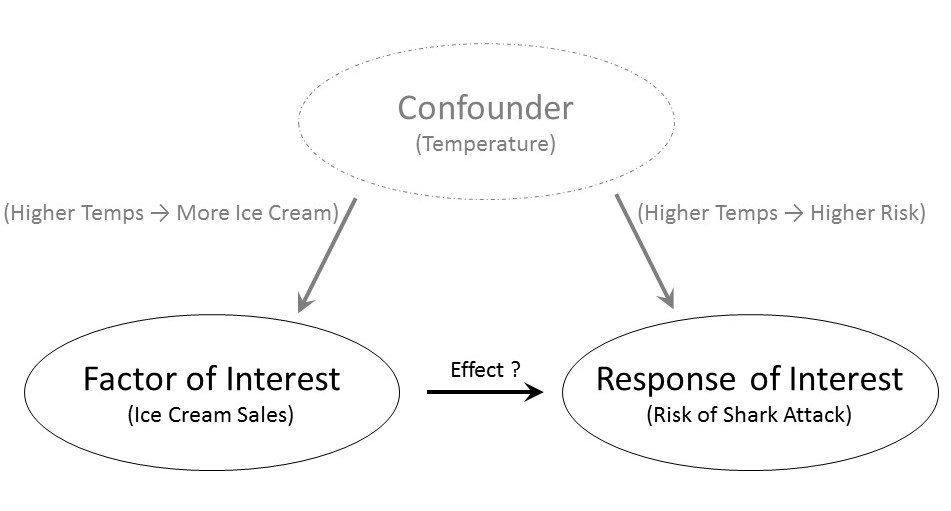
\includegraphics[width=0.8\textwidth,height=\textheight]{./images/Data-Confounding.jpg}

}

\caption{\label{fig-data-confounding}Illustration of a confounding
variable. The confounder, related to both the response and the factor of
interest (or treatment) can make it appear as though there is a causal
relationship when none exists.}

\end{figure}

\begin{tcolorbox}[enhanced jigsaw, leftrule=.75mm, coltitle=black, left=2mm, title=\textcolor{quarto-callout-tip-color}{\faLightbulb}\hspace{0.5em}{Big Idea}, breakable, toptitle=1mm, bottomtitle=1mm, colback=white, colbacktitle=quarto-callout-tip-color!10!white, titlerule=0mm, opacitybacktitle=0.6, colframe=quarto-callout-tip-color-frame, bottomrule=.15mm, arc=.35mm, opacityback=0, rightrule=.15mm, toprule=.15mm]

Confounders are variables that influence \emph{both} the factor of
interest and the response.

\end{tcolorbox}

Observational studies are subject to confounding; thus, controlled
experiments are often considered the gold standard in research because
they allow us to infer cause-and-effect relationships from the data.
Controlled experiments allow for causal interpretations because the
random allocation to the levels of the factor removes the impact of
confounders. Let's return to the hypothetical Vitamin-K study in
Example~\ref{exm-data-kangaroo}. Suppose there are nurses with a gentle
bedside manner and those who are a little less gentle. If we randomly
determine which infants receive Kangaroo Care, then for every gentle
nurse who is told to implement Kangaroo Care while giving the shot,
there tends to be a gentle nurse who is told to not implement Kangaroo
Care. Similarly, for every less-gentle nurse who is told to implement
Kangaroo Care while giving a shot, there tends to be a less-gentle nurse
who is told to not implement Kangaroo Care. This is illustrated in
Figure~\ref{fig-data-randomization}. For an observational study, the
treatment groups can be unbalanced; for example,
Figure~\ref{fig-data-randomization} illustrates a case in which there is
a higher fraction (11/12 compared to 1/4) of friendly nurses in the
Kangaroo Care group compared to the No Kangaroo Care group. For the
controlled experiment however, the treatment groups tend to be balanced
with respect to this confounder; there is approximately the same
fraction of friendly nurses in both groups. Random assignment is the
great equalizer. It tends to result in groups which are similar in all
respects; therefore, since we have eliminated all other differences
between the groups (other than the treatment they receive), any
differences we observe between the groups \emph{must} be due to the
grouping and not an underlying confounding variable.

\begin{figure}

{\centering 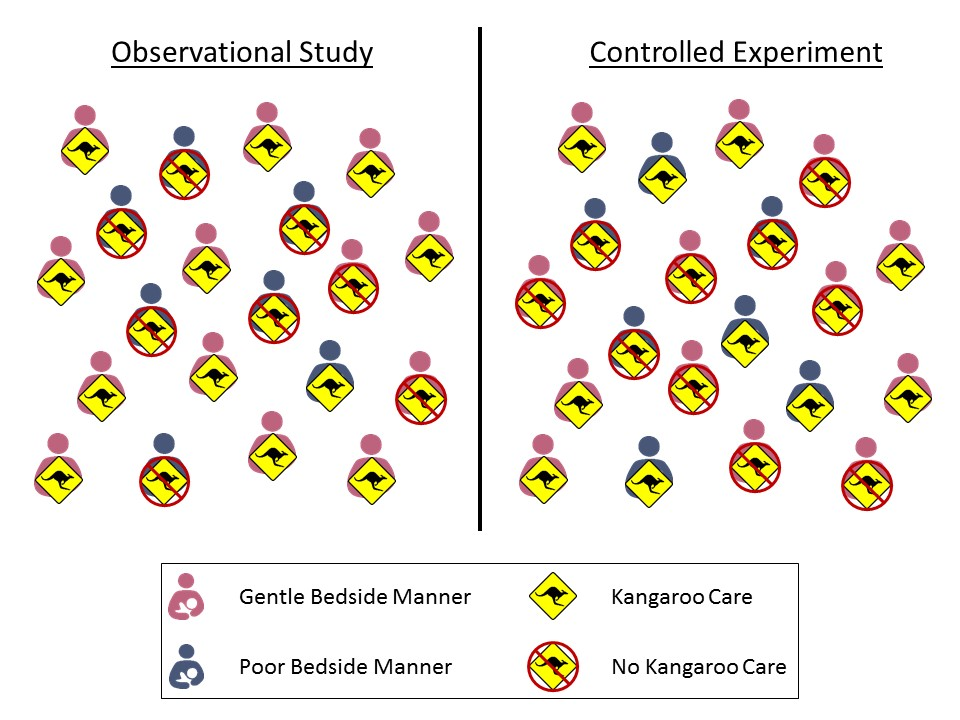
\includegraphics[width=0.8\textwidth,height=\textheight]{./images/Data-Randomization.jpg}

}

\caption{\label{fig-data-randomization}Illustration of the impact of
random assignment in study design. For the observational study, the
treatment groups are unbalanced. For the controlled experiment, the
treatment groups are balanced.}

\end{figure}

\begin{tcolorbox}[enhanced jigsaw, leftrule=.75mm, coltitle=black, left=2mm, title=\textcolor{quarto-callout-tip-color}{\faLightbulb}\hspace{0.5em}{Big Idea}, breakable, toptitle=1mm, bottomtitle=1mm, colback=white, colbacktitle=quarto-callout-tip-color!10!white, titlerule=0mm, opacitybacktitle=0.6, colframe=quarto-callout-tip-color-frame, bottomrule=.15mm, arc=.35mm, opacityback=0, rightrule=.15mm, toprule=.15mm]

Randomly assigning subjects to groups balances the groups with respect
to any confounders; that is, the groups being compared are similar.
Therefore, any differences between the two groups can be attributed to
the grouping itself, leading to cause-and-effect conclusions.

\end{tcolorbox}

While controlled experiments are a fantastic study design, we should not
discount the use of observational studies. Consider the Deepwater
Horizon Case Study described in Chapter~\ref{sec-caseDeepwater}; suppose
we are interested in the following question:

\begin{quote}
Is there evidence that volunteers who are directly exposed to oil have
an increased risk of developing adverse respiratory symptoms compared to
those who are not directly exposed to oil?
\end{quote}

The response is whether a volunteer develops adverse respiratory
symptoms; the factor of interest is whether the volunteer has direct
exposure to oil. We could conduct a controlled experiment by randomly
determining which volunteers are assigned to wildlife clean up and which
are assigned to administrative tasks, for example. However, it may be
that volunteer tasks need to be determined by skillset or by greatest
need at the time the person volunteers. It may not be feasible to
randomly assign volunteers to specific positions. Or, it could be that
the data was obtained after the fact; that is, the data is not the
result of a planned study in which case random assignment is not
possible because volunteers self-selected into positions in the past. If
random assignment is not possible, it does not mean the data is useless.
But, it does mean we will need to be sure we acknowledge, and
potentially address, the potential confounding when performing the
analysis and discussing the results.

The big idea is that in order to make causal conclusions, we must be
able to state that the groups being compared are balanced with respect
to any potential confounders; random assignment is one technique for
accomplishing this.

\hypertarget{aspects-of-a-well-designed-study}{%
\section{Aspects of a Well-Designed
Study}\label{aspects-of-a-well-designed-study}}

While controlled experiments are a useful tool, there are many aspects
to consider when designing a study. Generally speaking, there are three
components to a well-designed study: replication, randomization, and
reduction of extraneous noise.

\begin{tcolorbox}[enhanced jigsaw, leftrule=.75mm, coltitle=black, left=2mm, title=\textcolor{quarto-callout-warning-color}{\faExclamationTriangle}\hspace{0.5em}{Warning}, breakable, toptitle=1mm, bottomtitle=1mm, colback=white, colbacktitle=quarto-callout-warning-color!10!white, titlerule=0mm, opacitybacktitle=0.6, colframe=quarto-callout-warning-color-frame, bottomrule=.15mm, arc=.35mm, opacityback=0, rightrule=.15mm, toprule=.15mm]

A study is not poor just because it lacks one of these elements. That
is, a study can provide meaningful insights even if it did not make use
of each of these elements; every study is unique and should be designed
to address the research objective. These elements are simply helpful in
creating study designs.

\end{tcolorbox}

Variability is inherit in any process. We know there is variability in
the population; not every subject will respond exactly the same to each
treatment. Therefore, our questions do not seek to answer statements
about individuals but about general trends in the population. In order
to establish these general trends, we must allow that subject-to-subject
variability be present within the study itself. This is accomplished
through \textbf{replication}, obtaining data on multiple subjects from
each group. Each subject's response would be expected to be similar,
with variability within the group due to the inherent variability in the
data generating process.

\begin{definition}[Replication]\protect\hypertarget{def-replication}{}\label{def-replication}

Replication results from taking measurements on different units (or
subjects), for which you expect the results to be similar. That is, any
variability across the units is due to natural variability within the
population.

\end{definition}

\begin{tcolorbox}[enhanced jigsaw, leftrule=.75mm, coltitle=black, left=2mm, title=\textcolor{quarto-callout-warning-color}{\faExclamationTriangle}\hspace{0.5em}{Warning}, breakable, toptitle=1mm, bottomtitle=1mm, colback=white, colbacktitle=quarto-callout-warning-color!10!white, titlerule=0mm, opacitybacktitle=0.6, colframe=quarto-callout-warning-color-frame, bottomrule=.15mm, arc=.35mm, opacityback=0, rightrule=.15mm, toprule=.15mm]

The term ``replication'' is also used in the context of discussing
whether the results of a study are replicable. While our use of the term
is about replicating a measurement process within a study, this does not
downplay the importance of replicating an entire study.

\end{tcolorbox}

When we talk about gathering ``more data,'' we typically mean obtaining
a larger number of replicates. Ideally, replicates will be obtained
through \emph{random selection} from the underlying population to ensure
they are representative. The subjects are then \emph{randomly allocated}
to a particular level of the factor under study (randomly allocated to a
group) when performing a controlled experiment. This random allocation
breaks the link between the factor and any potential confounders,
allowing for causal interpretations. However, random allocation
preserves any link between the factor and the response, if a link
exists. These are the two aspects of \textbf{randomization}.

\begin{definition}[Randomization]\protect\hypertarget{def-randomization}{}\label{def-randomization}

Randomization can refer to random \emph{selection} or random
\emph{allocation}. Random selection refers to the use of a random
mechanism (e.g., a simple random sample,
Definition~\ref{def-simple-random-sample}, or a stratified random
sample, Definition~\ref{def-stratified-random-sample}) to select units
from the population. Random selection minimizes bias.

Random allocation refers to the use of a random mechanism when assigning
units to a specific treatment group in a controlled experiment
(Definition~\ref{def-controlled-experiment}). Random allocation
eliminates confounding and permits causal interpretations.

\end{definition}

\begin{tcolorbox}[enhanced jigsaw, leftrule=.75mm, coltitle=black, left=2mm, title=\textcolor{quarto-callout-note-color}{\faInfo}\hspace{0.5em}{Note}, breakable, toptitle=1mm, bottomtitle=1mm, colback=white, colbacktitle=quarto-callout-note-color!10!white, titlerule=0mm, opacitybacktitle=0.6, colframe=quarto-callout-note-color-frame, bottomrule=.15mm, arc=.35mm, opacityback=0, rightrule=.15mm, toprule=.15mm]

While those new to study design can typically describe random selection
and random allocation, they often confuse their purpose. Random
selection is to ensure the sample is representative. Random allocation
balances the groups with respect to confounders.

\end{tcolorbox}

It is tempting to manually adjust the treatment groups to achieve what
the researcher views as balance between the groups. This temptation
should be avoided as balancing one feature of the subjects may lead to
an imbalance in other features. Remember, random allocation leads to
balance. Of course, random allocation does not guarantee any particular
sample is perfectly balanced; however, any differences are due to chance
alone. As the sample size increases, these differences due to chance are
minimized.

Even with random allocation providing balance between the groups, there
will still be variability within each group. The more variability
present, the more difficult it is to detect a signal --- to discern a
difference in the mean response across groups. The study will more
easily detect the signal if the groups are similar. This leads to the
third component of a well-designed study --- the \textbf{reduction of
noise}.

\begin{definition}[Reduction of
Noise]\protect\hypertarget{def-noise-reduction}{}\label{def-noise-reduction}

Reducing extraneous sources of variability can be accomplished by fixing
extraneous variables or blocking (Definition~\ref{def-blocking}). These
actions reduce the number of differences between the units under study.

\end{definition}

\begin{tcolorbox}[enhanced jigsaw, leftrule=.75mm, coltitle=black, left=2mm, title=\textcolor{quarto-callout-note-color}{\faInfo}\hspace{0.5em}{Tension between Lab Settings and Reality}, breakable, toptitle=1mm, bottomtitle=1mm, colback=white, colbacktitle=quarto-callout-note-color!10!white, titlerule=0mm, opacitybacktitle=0.6, colframe=quarto-callout-note-color-frame, bottomrule=.15mm, arc=.35mm, opacityback=0, rightrule=.15mm, toprule=.15mm]

Scientists and engineers are trained to control unwanted sources of
variability (or sources of error in the data generating process). This
creates a tension between what is observed in the study (under ``lab''
settings) and what is observed in practice (in ``real-world'' settings).
This tension always exists, and the proper balance depends on the goals
of the researchers.

\end{tcolorbox}

Fixing the value of extraneous variables can reduce variability in a
study. For example, in Example~\ref{exm-data-kangaroo}, we might choose
to conduct the study at a single hospital. This choice impacts the value
of an extraneous variable. It is likely each hospital has its own
training process and protocols. The choice to only conduct the study at
a single hospital reduces the ``noise'' in how infants respond due to
different nurse behavior that reflects hospital training/protocol.
However, note that this decision also potentially limits the scope of
the study. It may not longer be appropriate to apply these results to
all hospitals.

An additional tool for reducing noise is \textbf{blocking}, in which
observations which are dependent on one another because of a shared
characteristic are grouped together.

\begin{definition}[Blocking]\protect\hypertarget{def-blocking}{}\label{def-blocking}

Blocking is a way of minimizing the variability contributed by an
inherent characteristic that results in dependent observations. In some
cases, the blocks are the unit of observation which is sampled from a
larger population, and multiple observations are taken on each unit. In
other cases, the blocks are formed by grouping the units of observations
according to an inherent characteristic; in these cases that shared
characteristic can be thought of having a value that was sampled from a
larger population.

In both cases, the observed blocks can be thought of as a random sample;
within each block, we have multiple observations, and the observations
from the same block are more similar than observations from different
blocks.

\end{definition}

\begin{example}[Overseeding Golf
Greens]\protect\hypertarget{exm-study-design-golf}{}\label{exm-study-design-golf}

Golf is a major pastime, especially in southern states. Each winter, the
putting greens need to be overseeded with grasses that will thrive in
cooler weather. This overseeding can affect how the ball rolls along the
green. Dudeck and Peeacock (1981) reports on an experiment that involved
comparing the ball roll for greens seeded with one of five varieties of
rye grass. Ball roll was measured by the mean distance (in meters) that
five balls traveled on the green. In order to induce a constant initial
velocity, each ball was rolled down an inclined plane.

Because the distance a ball rolls is influenced by the slope of the
green, 20 greens were placed into four groups in such a way that the
five greens in the same group had a similar slope. Then, within each of
these four groups, each of the five greens was randomly assigned to be
overseeded with one of the five types of Rye grass. The average ball
roll was recorded for each of the 20 greens.

\end{example}

The data from Example~\ref{exm-study-design-golf} are shown in
Table~\ref{tbl-study-design-golf-table}.

\hypertarget{tbl-study-design-golf-table}{}
\begin{table}
\caption{\label{tbl-study-design-golf-table}Data from the Overseeding Golf Greens example. }\tabularnewline

\centering
\begin{tabular}[t]{llr}
\toprule
Rye Grass Variety & Slope of Green Grouping & Mean Distance Traveled (m)\\
\midrule
\cellcolor{gray!6}{A} & \cellcolor{gray!6}{1} & \cellcolor{gray!6}{2.764}\\
B & 1 & 2.568\\
\cellcolor{gray!6}{C} & \cellcolor{gray!6}{1} & \cellcolor{gray!6}{2.506}\\
D & 1 & 2.612\\
\cellcolor{gray!6}{E} & \cellcolor{gray!6}{1} & \cellcolor{gray!6}{2.238}\\
\addlinespace
A & 2 & 3.043\\
\cellcolor{gray!6}{B} & \cellcolor{gray!6}{2} & \cellcolor{gray!6}{2.977}\\
C & 2 & 2.533\\
\cellcolor{gray!6}{D} & \cellcolor{gray!6}{2} & \cellcolor{gray!6}{2.675}\\
E & 2 & 2.616\\
\addlinespace
\cellcolor{gray!6}{A} & \cellcolor{gray!6}{3} & \cellcolor{gray!6}{2.600}\\
B & 3 & 2.183\\
\cellcolor{gray!6}{C} & \cellcolor{gray!6}{3} & \cellcolor{gray!6}{2.334}\\
D & 3 & 2.164\\
\cellcolor{gray!6}{E} & \cellcolor{gray!6}{3} & \cellcolor{gray!6}{2.127}\\
\addlinespace
A & 4 & 3.049\\
\cellcolor{gray!6}{B} & \cellcolor{gray!6}{4} & \cellcolor{gray!6}{3.028}\\
C & 4 & 2.895\\
\cellcolor{gray!6}{D} & \cellcolor{gray!6}{4} & \cellcolor{gray!6}{2.724}\\
E & 4 & 2.697\\
\bottomrule
\end{tabular}
\end{table}

It would have been easy to simply assign 4 greens to each of the Rye
grass varieties; the random allocation would have balanced any
confounders across the five varieties. However, an additional layer was
added to the design in order to control some of that additional
variability. In particular, greens with similar slopes were grouped
together; then, the random allocation to Rye grass varieties happened
\emph{within} the grouped greens. The blocks in this study are the
``slope groups.'' Each block represents greens with a different slope.
Certainly, there are more than 4 potential slopes that a green might
have; yet, we observed 4 such groups in our study. We can think of these
4 observed slopes as a sample of all slopes that might exist on a
putting green.

Within each block, we have five units of observations; these five units
were randomized to the five treatment groups (the five Rye grass
varieties). Notice the random allocation strategy ensures that each
variety appears exactly once within each slope grouping. This study
design will allow us to compare the impact of the Rye grass variety
while minimizing the extraneous variability due to the slope of the
green, which is a nuisance characteristic. To see how we capitalize on
blocking in the analysis, we refer you to Unit IV of the text.

\begin{tcolorbox}[enhanced jigsaw, leftrule=.75mm, coltitle=black, left=2mm, title=\textcolor{quarto-callout-note-color}{\faInfo}\hspace{0.5em}{Note}, breakable, toptitle=1mm, bottomtitle=1mm, colback=white, colbacktitle=quarto-callout-note-color!10!white, titlerule=0mm, opacitybacktitle=0.6, colframe=quarto-callout-note-color-frame, bottomrule=.15mm, arc=.35mm, opacityback=0, rightrule=.15mm, toprule=.15mm]

Blocking is often a way of gaining additional power when limited
resources require your study to have a small sample size.

\end{tcolorbox}

An extreme case of blocking occurs when you repeatedly measure the
response on the same subject under different treatment conditions. For
example, a pre-test/post-test study is an example of a study which
incorporates blocking. In this case, the blocks are the individual
subjects, the unit of observation. The response is then observed on the
subject both prior to the intervention (the ``test'') and following the
intervention. The rationale here is to use every subject as his or her
own ``control.'' This reduces extraneous noise because the two treatment
groups (the pre-test group and the post-test group) are identical.

\begin{tcolorbox}[enhanced jigsaw, leftrule=.75mm, coltitle=black, left=2mm, title=\textcolor{quarto-callout-tip-color}{\faLightbulb}\hspace{0.5em}{Big Idea}, breakable, toptitle=1mm, bottomtitle=1mm, colback=white, colbacktitle=quarto-callout-tip-color!10!white, titlerule=0mm, opacitybacktitle=0.6, colframe=quarto-callout-tip-color-frame, bottomrule=.15mm, arc=.35mm, opacityback=0, rightrule=.15mm, toprule=.15mm]

A block is a secondary grouping variable present during the data
collection that records a nuisance characteristic. While it reduces
extraneous noise in the sample, the block must be accounted for
appropriately during the analysis of the data (as described in
Chapter~\ref{sec-dependent-groups}).

\end{tcolorbox}

\hypertarget{collecting-observational-data}{%
\section{Collecting Observational
Data}\label{collecting-observational-data}}

An inability to conduct a controlled experiment does not mean we neglect
study design. Random sampling is still helpful in ensuring that the data
is representative of the population. And, even if random sampling is not
feasible, we should still aim to minimize bias and have a sample that is
representative of our population. Similarly, ensuring there are a
sufficient number of replications to capture the variability within the
data is an important aspect of conducting an observational study. When
collecting observational data, one of the most important steps is
constructing a list of potential confounders and then collecting data on
these variables as well. This will allow us to account for these
confounders in our analysis (see Chapter~\ref{sec-reg-extensions}); we
cannot model what we do not collect. Finally, observational studies may
still permit the blocking of subjects and accounting for this additional
variability in our analysis.

\hypertarget{sec-independent-groups}{%
\chapter{Considerations when Comparing Independent
Groups}\label{sec-independent-groups}}

\providecommand{\norm}[1]{\lVert#1\rVert}
\providecommand{\abs}[1]{\lvert#1\rvert}
\providecommand{\iid}{\stackrel{\text{IID}}{\sim}}
\providecommand{\ind}{\stackrel{\text{Ind}}{\sim}}

\providecommand{\bm}[1]{\mathbf{#1}}
\providecommand{\bs}[1]{\boldsymbol{#1}}
\providecommand{\bbeta}{\bs{\beta}}

\providecommand{\Ell}{\mathcal{L}}
\providecommand{\indep}{\perp\negthickspace\negmedspace\perp}

While the approaches we have described in the text have been general, we
have generally assumed we were modeling a single variable from a single
population. That is, we were interested in characterizing the data
generating process for a response \(Y\); specifically, we assumed the
density \(f(y \mid \boldsymbol{\theta})\) depended on unknown parameters
\(\boldsymbol{\theta}\). We would use a random sample
\(Y_1, Y_2, \dots, Y_n\) from this population to make inference on those
parameters. Many questions do not fit into that mold.

\begin{example}[Distracted
Driving]\protect\hypertarget{exm-distracted-driving}{}\label{exm-distracted-driving}

Nearly every state in the US has a restriction on cell phone use while
driving. Some states prohibit texting while driving, while states like
Indiana only permit hands-free use of a phone. The goal of these
regulations is to reduce distractions while driving and thereby improve
reaction time.

\end{example}

Does cell phone use reduce reaction time? Does it increase the
likelihood of a collision? These questions seek to compare a response
(the reaction time) across groups formed by the predictor (cell phone
use or not). There are two ways to conceptually think about this
comparison. First, we could think of there being two independent
populations --- those who use cell phones while driving, and those who
do not use cell phones while driving. In this perspective, we are
interested in comparing these two populations, and we imagine sampling
from each population separately. Alternatively, we could think of there
being a single population (those who drive) exposed to two different
treatments (using cell phones and not using cell phones). In this
perspective, we are interested in comparing the impact of the treatments
on the response, and we imagine sampling from the single population and
then each unit being allocated one of the treatment groups. While the
details are different between these two perspectives, mathematically,
they are equivalent.

Let's first consider the perspective of two independent populations.
Specifically, let \(Y_{j,i}\) be the response for the \(i\)-th
observation in population \(j\), \(i = 1, 2, \dotsc, n_j\), where
\(n_j\) is the number of subjects observed from population \(j\) and
\(j = 1, 2, \dotsc, J\), where \(J\) is the number of populations being
compared. Further, we assume
\(Y_{j, i} \stackrel{IID}{\sim} f_j\left(y \mid \boldsymbol{\theta}_j\right)\);
that is, we have a random sample from each population. Notice that we
are potentially allowing the form of the data generating process \(f\)
to vary for each population; and, we certainly allow the parameters
\(\boldsymbol{\theta}\) to vary for each population. Since we consider
each sample independent of one another, we have that the likelihood has
the form

\begin{equation}\protect\hypertarget{eq-ind-groups-likelihood1}{}{f(\mathbf{y} \mid \boldsymbol{\theta}) = \prod_{j=1}^{J} \prod_{i=1}^{n_j} f_j\left(y_{j, i} \mid \boldsymbol{\theta}_j\right).}\label{eq-ind-groups-likelihood1}\end{equation}

It now remains to specify a prior on each \(\boldsymbol{\theta}_j\). Of
course, if the groups are independent of one another, it is also
reasonable to assume the parameters are independent of one another. This
leads to

\begin{equation}\protect\hypertarget{eq-ind-groups-prior1}{}{\pi(\boldsymbol{\theta}) = \prod_{j=1}^{J} \pi_j(\boldsymbol{\theta}_j).}\label{eq-ind-groups-prior1}\end{equation}

Now let's consider the perspective of a single population exposed to two
treatments. Specifically, let \(Y_i\) be the response for the \(i\)-th
observation in the population, and we let \(x_i\) be a variable that
indicates to which treatment the \(i\)-th observation has been exposed;
that is, \(x_i = j\) if the \(i\)-th observation has been exposed to the
\(j\)-th treatment. We then have that
\(Y_i \stackrel{Ind}{\sim} f\left(y \mid \boldsymbol{\theta}_{x_i}\right)\).
Notice that we do not say that the responses are identically
distributed; while the family of distributions is the same (all have the
same \(f\)), the parameters on which each distribution depends is
allowed to differ (based on the value of \(x_i\)). Therefore, we are
only willing to say the observations are independent. The likelihood
then has the form

\begin{equation}\protect\hypertarget{eq-ind-groups-likelihood2}{}{f(\mathbf{y} \mid \boldsymbol{\theta}) = \prod_{i=1}^{n} f\left(y \mid \boldsymbol{\theta}_{x_i}\right).}\label{eq-ind-groups-likelihood2}\end{equation}

It now remains to specify a prior on each \(\boldsymbol{\theta}_j\). If
we are willing to assume the treatment groups are independent of one
another, it is also reasonable to assume the parameters are independent
of one another. This leads to

\begin{equation}\protect\hypertarget{eq-ind-groups-prior2}{}{\pi(\boldsymbol{\theta}) = \prod_{j=1}^{J} \pi_j(\boldsymbol{\theta}_j).}\label{eq-ind-groups-prior2}\end{equation}

Equation~\ref{eq-ind-groups-likelihood1} and
Equation~\ref{eq-ind-groups-likelihood2} are equivalent models for the
likelihood; similarly, Equation~\ref{eq-ind-groups-prior1} and
Equation~\ref{eq-ind-groups-prior2} are equivalent models for the prior.

\begin{tcolorbox}[enhanced jigsaw, leftrule=.75mm, coltitle=black, left=2mm, title=\textcolor{quarto-callout-note-color}{\faInfo}\hspace{0.5em}{Note}, breakable, toptitle=1mm, bottomtitle=1mm, colback=white, colbacktitle=quarto-callout-note-color!10!white, titlerule=0mm, opacitybacktitle=0.6, colframe=quarto-callout-note-color-frame, bottomrule=.15mm, arc=.35mm, opacityback=0, rightrule=.15mm, toprule=.15mm]

When comparing groups, whether you view the groups as separate
populations or a single population exposed to different treatments, the
inference is the same provided the groups are independent.

\end{tcolorbox}

\begin{tcolorbox}[enhanced jigsaw, leftrule=.75mm, coltitle=black, left=2mm, title=\textcolor{quarto-callout-tip-color}{\faLightbulb}\hspace{0.5em}{Big Idea}, breakable, toptitle=1mm, bottomtitle=1mm, colback=white, colbacktitle=quarto-callout-tip-color!10!white, titlerule=0mm, opacitybacktitle=0.6, colframe=quarto-callout-tip-color-frame, bottomrule=.15mm, arc=.35mm, opacityback=0, rightrule=.15mm, toprule=.15mm]

In order to extend inference from a single variable to comparing groups,
we essentially allow our parameters to be based on the group from which
the data was taken. That is, we add a second layer to our model.

\end{tcolorbox}

\begin{example}[C-Section Deliveries
Continued]\protect\hypertarget{exm-csec-independent-groups}{}\label{exm-csec-independent-groups}

Example~\ref{exm-csec} introduced a study, a component of which includes
estimating the probability of a mother undergoing a C-section delivery
at a particular hospital. That example focused on estimating the
C-section rate at a particular hospital. However, there are two
hospitals in Terre Haute, Indiana. Suppose we are now interested in
extending the study to compare the rate of C-sections at the two
hospitals.

Develop a suitable model for addressing this new research objective.

\end{example}

\begin{solution}

Let \(Y_{j, i}\) denote the number of vaginal deliveries at hospital
\(j\) prior to the \(i\)-th C-section we observe at hospital \(j\).
Further, let \(\theta_j\) denote the rate of C-sections at hospital
\(j\); our interest is in comparing \(\theta_1\) and \(\theta_2\).
Following the discussion of Example~\ref{exm-csec}, we have that

\[Pr\left(Y_{j,i} = y\right) = \theta_j \left(1 - \theta_j\right)^y \qquad y = 0, 1, 2, \dotsc.\]

Further, it is reasonable to assume that whether a mother undergoes a
C-section at one hospital is unrelated to whether a mother undergoes a
C-section at the other hospital. Therefore, we can consider \(Y_{1,i}\)
to be independent of \(Y_{2,k}\) for all choices of \(i\) and \(k\).
And, since each birth is independent, we can consider
\(Y_{j,1}, Y_{j,2}, \dotsc, Y_{j, n}\) to be a random sample from the
\(j\)-th hospital. Note that while we have set \(n\) to be the same for
both hospitals, this is not a requirement.

Letting
\(\mathbf{Y} = \left(Y_{1,1}, Y_{1,2}, \dotsc, Y_{1,n}, Y_{2, 1}, Y_{2, 2}, \dotsc, Y_{2, n}\right)^\top\)
be the random vector of observations, the likelihood is given by

\begin{equation}\protect\hypertarget{eq-csec-ind-likelihood}{}{
\begin{aligned}
  f(\mathbf{y} \mid \boldsymbol{\theta})
    &= \prod_{j=1}^{2} \prod_{i=1}^{n} f_{Y_{j,i}}\left(y_{j,i} \mid \theta_j\right) \\
    &= \prod_{j=1}^{2} \prod_{i=1}^{n} \theta_j \left(1 - \theta_j\right)^{y_{j,i}} \\
    &= \prod_{j=1}^{2} \theta_j^n \left(1 - \theta_j\right)^{\sum_{i=1}^{n} y_{j,i}} \\
    &= \theta_1^n \left(1 - \theta_1\right)^{n\bar{y}_1} \theta_2^n \left(1 - \theta_2\right)^{n\bar{y}_2}, 
\end{aligned}
}\label{eq-csec-ind-likelihood}\end{equation}

where \(\bar{y}_j\) represents the observed sample mean for hospital
\(j\). We note that the likelihood expressly captures both populations
and therefore acknowledges the dependence on the both parameters.

We now consider developing a prior distribution. Since \(\theta_j\) is a
probability, it seems reasonable to choose a Beta distribution for each
parameter. Further, if we believe the parameters are independent, the
prior distribution is

\[\pi(\boldsymbol{\theta}) = \frac{\Gamma\left(a_1 + b_1\right)}{\Gamma\left(a_1\right)\Gamma\left(b_1\right)} \theta_1^{a_1 - 1}\left(1 - \theta_1\right)^{b_1 - 1}\frac{\Gamma\left(a_2 + b_2\right)}{\Gamma\left(a_2\right)\Gamma\left(b_2\right)} \theta_2^{a_2 - 1}\left(1 - \theta_2\right)^{b_2 - 1}.\]

Notice that our choice of prior allows the hyperparameters to
potentially differ for each hospital.

\end{solution}

\hypertarget{bridge-sampling}{%
\section{Bridge Sampling}\label{bridge-sampling}}

In Chapter~\ref{sec-hypothesis-testing} we introduced the idea of model
comparison. This is especially useful when comparing groups. Consider a
simple case in which we have two groups. Specifically, suppose

\[
\begin{aligned}
  Y_{1,i} &\stackrel{IID}{\sim} f(y \mid \theta_1) \\
  Y_{2,i} &\stackrel{IID}{\sim} f(y \mid \theta_2) \\
  Y_{1,i} &\perp\negthickspace\negmedspace\perp Y_{2,j} \quad \forall i, j
\end{aligned}
\]

where \(\perp\negthickspace\negmedspace\perp\) refers to independence.
In this example, the data generating process for each group is
distinguished only by a potentially different value of the parameter. It
would be natural in such settings to consider the hypotheses

\[H_0: \theta_1 = \theta_2 \qquad \text{vs.} \qquad H_1: \theta_1 \neq \theta_2.\]

If we place a continuous prior on the parameters, then the probability
of \(H_0\) must be 0. One way of addressing this problem is to consider
a clever prior which places mass along the \emph{line} equating the two
parameters. A more natural solution, however, is to think of this as a
model comparison problem:

\[
\begin{aligned}
  \mathcal{M}_0:& \quad Y_{j, i} \stackrel{IID}{\sim} f(y \mid \theta) \\
    & \quad \theta \sim \pi_0(\theta) \\
  \mathcal{M}_1:& \quad Y_{j, i} \stackrel{Ind}{\sim} f(y \mid \theta_j) \\
    & \quad \theta_j \stackrel{Ind}{\sim} \pi_j(\theta_j)
\end{aligned}
\]

for \(j = 1, 2\). Notice that under model \(\mathcal{M}_0\), there is
only a single parameter, capturing the null hypothesis
\(\theta_1 = \theta_2\). And, model \(\mathcal{M}_1\) allows the
flexibility for two parameters, capturing the alternative hypothesis. We
would therefore be interested in computing a Bayes Factor (see
Definition~\ref{def-bayes-factor}) comparing these two models. The
problem is, the Bayes Factor depends on the evidence

\[f(\mathbf{y} \mid \mathcal{M}_j) = \int f(\mathbf{y} \mid \boldsymbol{\theta}, \mathcal{M}_j) \pi(\boldsymbol{\theta} \mid \mathcal{M}_j) d\boldsymbol{\theta}.\]

Unfortunately, this integral is quite difficult to estimate. Using the
prior distribution and performing MC Integration techniques does not
typically result in reliable estimation; this results from the prior
distribution often being too vague. Instead, the evidence is estimated
from the posterior distribution using \textbf{bridge sampling}.

\begin{definition}[Bridge
Sampling]\protect\hypertarget{def-bridge-sampling}{}\label{def-bridge-sampling}

The bridge sampling estimator of the marginal likelihood
\(m(\mathbf{y})\) is given by

\[
\begin{aligned}
  m(\mathbf{y}) 
    &= \int f(\mathbf{y} \mid \boldsymbol{\theta}) \pi(\boldsymbol{\theta}) d\boldsymbol{\theta} \\
    &= \frac{E_g\left[h(\boldsymbol{\theta}) f(\mathbf{y} \mid \boldsymbol{\theta}) \pi(\boldsymbol{\theta})\right]}{E_{\pi}\left[h(\boldsymbol{\theta}) g(\boldsymbol{\theta}) \right]} \\
    &\approx \frac{m^{-1}\sum_{j=1}^{m} h\left(\tilde{\boldsymbol{\theta}}_j\right) f\left(\mathbf{y} \mid \tilde{\boldsymbol{\theta}}_j\right) \pi\left(\tilde{\boldsymbol{\theta}}_j\right)}{m^{-1}\sum_{i=1}^{m} h\left(\boldsymbol{\theta}^*_j\right) g\left(\boldsymbol{\theta}^*_j\right)}
\end{aligned}
\]

where \(h(\boldsymbol{\theta})\) is called the bridge function and
\(g(\boldsymbol{\theta})\) is the proposal distribution. Here,
\(\tilde{\boldsymbol{\theta}}\) denotes a random variate from the
proposal distribution and \(\boldsymbol{\theta}^*\) a random variate
from the posterior; \(E_g\) denotes taking an expectation with respect
to the proposal distribution and \(E_\pi\) denotes taking an expectation
with respect to the posterior distribution.

\end{definition}

\begin{tcolorbox}[enhanced jigsaw, leftrule=.75mm, coltitle=black, left=2mm, title=\textcolor{quarto-callout-note-color}{\faInfo}\hspace{0.5em}{Note}, breakable, toptitle=1mm, bottomtitle=1mm, colback=white, colbacktitle=quarto-callout-note-color!10!white, titlerule=0mm, opacitybacktitle=0.6, colframe=quarto-callout-note-color-frame, bottomrule=.15mm, arc=.35mm, opacityback=0, rightrule=.15mm, toprule=.15mm]

While not required, it is typical to use a Normal distribution for the
proposal distribution \(g(\boldsymbol{\theta})\).

\end{tcolorbox}

Bridge sampling is available in some software packages (such as R, for
example). While the details of bridge sampling are beyond the scope of
this text, we do want to note that the definition comes from making the
following observation:

\[
\begin{aligned}
  1 &= \frac{\int f(\mathbf{y} \mid \boldsymbol{\theta}) \pi(\boldsymbol{\theta}) g(\boldsymbol{\theta}) h(\boldsymbol{\theta})d\boldsymbol{\theta}}{\int f(\mathbf{y} \mid \boldsymbol{\theta}) \pi(\boldsymbol{\theta}) g(\boldsymbol{\theta}) h(\boldsymbol{\theta})d\boldsymbol{\theta}} \\
  \Rightarrow m(\mathbf{y}) &= m(\mathbf{y}) \frac{\int f(\mathbf{y} \mid \boldsymbol{\theta}) \pi(\boldsymbol{\theta}) g(\boldsymbol{\theta}) h(\boldsymbol{\theta})d\boldsymbol{\theta}}{\int f(\mathbf{y} \mid \boldsymbol{\theta}) \pi(\boldsymbol{\theta}) g(\boldsymbol{\theta}) h(\boldsymbol{\theta})d\boldsymbol{\theta}}. 
\end{aligned}
\]

We are able to multiply both sides by the prior predictive distribution
because it will be non-negative on its support. Next, recognize that the
integral is with respect to \(\boldsymbol{\theta}\); therefore, we can
move the marginal distribution inside the integral in the denominator to
get

\[
\begin{aligned}
  m(\mathbf{y}) &= \frac{\int f(\mathbf{y} \mid \boldsymbol{\theta}) \pi(\boldsymbol{\theta}) h(\boldsymbol{\theta}) g(\boldsymbol{\theta})d\boldsymbol{\theta}}{\int \frac{f(\mathbf{y} \mid \boldsymbol{\theta}) \pi(\boldsymbol{\theta})}{m(\mathbf{y})} h(\boldsymbol{\theta}) g(\boldsymbol{\theta})d\boldsymbol{\theta}} \\
    &= \frac{\int f(\mathbf{y} \mid \boldsymbol{\theta}) \pi(\boldsymbol{\theta}) h(\boldsymbol{\theta}) g(\boldsymbol{\theta})d\boldsymbol{\theta}}{\int \pi(\boldsymbol{\theta} \mid \mathbf{y}) h(\boldsymbol{\theta}) g(\boldsymbol{\theta})d\boldsymbol{\theta}},
\end{aligned}
\]

where the last equality makes use of the definition of the posterior
distribution from Bayes Theorem. Now, the top integral can be viewed in
terms of an expectation over a random variable
\(\boldsymbol{\theta} \sim g(\boldsymbol{\theta})\), and the denominator
can be viewed as an expectation over a random variable which follows the
posterior distribution.

\begin{tcolorbox}[enhanced jigsaw, leftrule=.75mm, coltitle=black, left=2mm, title=\textcolor{quarto-callout-tip-color}{\faLightbulb}\hspace{0.5em}{Big Idea}, breakable, toptitle=1mm, bottomtitle=1mm, colback=white, colbacktitle=quarto-callout-tip-color!10!white, titlerule=0mm, opacitybacktitle=0.6, colframe=quarto-callout-tip-color-frame, bottomrule=.15mm, arc=.35mm, opacityback=0, rightrule=.15mm, toprule=.15mm]

Bridge sampling is an efficient algorithm for estimating the evidence of
a model, allowing for computation of the Bayes Factor.

\end{tcolorbox}

\hypertarget{sec-dependent-groups}{%
\chapter{Considerations when Comparing Related
Groups}\label{sec-dependent-groups}}

\providecommand{\norm}[1]{\lVert#1\rVert}
\providecommand{\abs}[1]{\lvert#1\rvert}
\providecommand{\iid}{\stackrel{\text{IID}}{\sim}}
\providecommand{\ind}{\stackrel{\text{Ind}}{\sim}}

\providecommand{\bm}[1]{\mathbf{#1}}
\providecommand{\bs}[1]{\boldsymbol{#1}}
\providecommand{\bbeta}{\bs{\beta}}

\providecommand{\Ell}{\mathcal{L}}
\providecommand{\indep}{\perp\negthickspace\negmedspace\perp}

The previous chapter was a natural extension of the framework we had
developed in earlier portions of the text. Assuming each group is
independent, we were essentially able to model each group separately;
the likelihood was then the product of the likelihoods from each group,
and the prior was the product of the priors from each group. This
independence will actually carry through into the posterior
distribution. That is, the independence allows us to model the groups
separately and then combine afterwards. However, independence between
the groups is not always reasonable.

Recall that one of the aspects of a good study design is comparative
groups --- treatment groups which are similar except for the treatment
being applied. The benefit of this is that it reduces extraneous
variability. We also saw that blocking (Definition~\ref{def-blocking})
is a useful strategy for reducing extraneous variability that groups
together observations which share some inherent characteristic. A very
common example of blocking is a pre/post test. In such settings,
participants are given a baseline assessment. Then, each participant is
exposed to some form of treatment; following this, participants take an
another assessment. Interest is typically on quantifying the change from
baseline.

In this case, the two groups (pre-treatment and post-treatment) are not
only similar, they are identical! Intuitively, this is a good design
because we are allowing every individual to act as their own control. We
have eliminated all other external sources of variability allowing us to
focus on the treatment of interest. Here, the individual participants
act as the blocks. In such cases, we believe the variability among
observations between blocks is greater than the variability among
observations within a block. Unfortunately, this causes a relationship
among the observations, meaning it is no longer reasonable to assume the
observations are independent of one another.

\begin{tcolorbox}[enhanced jigsaw, leftrule=.75mm, coltitle=black, left=2mm, title=\textcolor{quarto-callout-tip-color}{\faLightbulb}\hspace{0.5em}{Big Idea}, breakable, toptitle=1mm, bottomtitle=1mm, colback=white, colbacktitle=quarto-callout-tip-color!10!white, titlerule=0mm, opacitybacktitle=0.6, colframe=quarto-callout-tip-color-frame, bottomrule=.15mm, arc=.35mm, opacityback=0, rightrule=.15mm, toprule=.15mm]

When subjects can be blocked (or pooled) into similar groups,
independence is no longer reasonable.

\end{tcolorbox}

When we believe there are clusters of related observations, we lean on
the hierarchical nature of the data generating process, and this allows
us to construct the likelihood.

\begin{example}[Final
Exams]\protect\hypertarget{exm-exams}{}\label{exm-exams}

Common final exams are typical for multiple sections of the same course
at a university. For example, there may be four instructors, each
teaching two sections of Calculus; all eight sections will receive the
same final exam. Suppose each exam is graded out of 100 points and we
are interested in modeling the exam score for students taking the exam.

\end{example}

We might start off by assuming a common distribution for all students.
That is,

\[
\begin{aligned}
  Y_i \mid \boldsymbol{\theta} &\stackrel{IID}{\sim} f(y \mid \boldsymbol{\theta}) \\
  \theta &\sim \pi(\theta).
\end{aligned}
\]

where \(Y_i\) is the exam score for the \(i\)-th subject. However, this
model is imposing a particular assumption --- there are no differences
among instructors that would impact the scores of the students.
Essentially, every instructor delivers the same content in the same way
suggesting the students might has well have been taught by the same
instructor. While this is a nice ideal, it is typically not the case.
Autonomy in the classroom means that different instructors approach the
material differently --- emphasizing different topics and presenting the
material in different ways. As a result, it is possible that students
who share an instructor are more likely to perform well on the same
types of problems and also more likely to make the same types of
mistakes (compared with students who do not share the same instructor).
The additional variability introduced by the differences across
instructors is being ignored in this model.

We might try to correct for this by assuming the instructors are
completely independent of one another, following the approach of the
previous chapter. This would say

\[
\begin{aligned}
  Y_{j, i} \mid \boldsymbol{\theta}_j &\stackrel{IID}{\sim} f(y \mid \boldsymbol{\theta}_j) \\
  Y_{r, s} &\perp\negthickspace\negmedspace\perp Y_{t, u} \quad \forall r, s, t, u \\
  \boldsymbol{\theta}_j &\stackrel{Ind}{\sim} \pi_j(\boldsymbol{\theta}_j).
\end{aligned}
\]

However, this model has very limited utility in practice. If we wanted
to predict the exam score of a student taking calculus, our model would
only be applicable if they were taking it with one of \emph{these} four
instructors! Given another student, we would need to know which of these
instructors they were taking the course with in order to know which of
the four parameters to lean on in predicting their score. That is, this
model inherently compares instructors; but, we do not actually care
about comparing Instructor 1 and Instructor 2. Further, the next time
the course is offered, there are likely to be four completely new
instructors, and we want our model to be accommodate this. Perhaps more
importantly, we do not actually think the instructors are completely
unrelated (they are teaching the same major content after all\ldots at
least, we would hope so). So, this extreme perspective also seems to
ignore the structure in the problem.

\begin{tcolorbox}[enhanced jigsaw, leftrule=.75mm, coltitle=black, left=2mm, title=\textcolor{quarto-callout-tip-color}{\faLightbulb}\hspace{0.5em}{Big Idea}, breakable, toptitle=1mm, bottomtitle=1mm, colback=white, colbacktitle=quarto-callout-tip-color!10!white, titlerule=0mm, opacitybacktitle=0.6, colframe=quarto-callout-tip-color-frame, bottomrule=.15mm, arc=.35mm, opacityback=0, rightrule=.15mm, toprule=.15mm]

How we model the relationship between groups, if one exists at all, must
be based on the context of the problem.

\end{tcolorbox}

It seems natural to think of these four instructors as a representative
sample from a population of all potential instructors. That is, we are
adding a layer to the data generating process. First, instructors are
chosen to teach the course; then, students are placed with an
instructor, impacting their performance on the final exam. The way these
instructors impact the data generating process is through the formation
of the parameters \(\boldsymbol{\theta}_j\). Therefore, we incorporate
this into the model. Specifically, consider

\[
\begin{aligned}
  Y_{j, i} \mid \boldsymbol{\theta}_j &\stackrel{IID}{\sim} f(y \mid \boldsymbol{\theta}_j) \\
  \boldsymbol{\theta}_j \mid \boldsymbol{\eta} &\stackrel{IID}{\sim} \pi(\boldsymbol{\theta} \mid \boldsymbol{\eta}) \\
  \boldsymbol{\eta} &\sim \pi(\boldsymbol{\eta}).
\end{aligned}
\]

This model has three layers:

\begin{itemize}
\tightlist
\item
  Layer 1: Describes how students \emph{within} an instructor perform;
  the parameters are unique to each instructor but shared across
  students with the same instructor.
\item
  Layer 2: Describes the variability \emph{across} instructors; treating
  the instructors as a random sample of all instructors, we allow the
  parameters to move across instructors according to some overall model.
\item
  Layer 3: Describes our prior beliefs about the shared parameters for
  the instructor-level model.
\end{itemize}

This hierarchical model bridges the gap between ignoring the blocks and
treating the blocks as independent groups. This allows us to pool
information similar across blocks while allowing unique properties to
exist for each block as well.

\begin{tcolorbox}[enhanced jigsaw, leftrule=.75mm, coltitle=black, left=2mm, title=\textcolor{quarto-callout-note-color}{\faInfo}\hspace{0.5em}{Hierarchical Approach to Addressing Dependence}, breakable, toptitle=1mm, bottomtitle=1mm, colback=white, colbacktitle=quarto-callout-note-color!10!white, titlerule=0mm, opacitybacktitle=0.6, colframe=quarto-callout-note-color-frame, bottomrule=.15mm, arc=.35mm, opacityback=0, rightrule=.15mm, toprule=.15mm]

When the dependence in data is the result of a hierarchical data
generating process, we can incorporate that additional variability by
modeling the hierarchical structure directly. At a minimum, this has the
following three layers:

\begin{itemize}
\tightlist
\item
  Layer 1: Describes how observations \emph{within} a block behave; with
  parameters unique to each block.
\item
  Layer 2: Describes how the parameters move \emph{across} blocks; this
  views the blocks as a random sample.
\item
  Layer 3: Describes our prior beliefs on the common parameters for the
  model in Layer 2.
\end{itemize}

\end{tcolorbox}

It is natural to question the difference between a block and a factor
(or the grouping comparison that we considered in the previous chapter).
The difference is primarily in how we address them in the modeling. If
we are interested in making group-to-group comparisons, and if the
groups would remain the same when repeating the study, the variable
should be treated as a factor of interest. If the groups primarily
capture an additional source of variability and can be viewed as a
random sample from some larger population, the variable should be
treated as a block.

Of course, we can combine the two ideas in a single study. Suppose
further that we were interested in comparing students majoring in
mathematics and those not majoring in mathematics. The first layer of
the model must still describe what happens within a block (or within an
instructor in our example). The assumptions you are willing to make
determine how complex this becomes. For example, assuming that the
difference between mathematics majors and non-mathematics majors is
similar regardless of the instructor implies that mathematics majors
share some common parameter across instructors. However, allowing the
difference to vary across instructors implies that there is no common
parameter. This is addressed within the first two layers of the model.
If the effect is held constant across the blocks, a single set of
``global'' parameters enters into Layer 1 for which priors are described
in Layer 3. If the effect is allowed to vary, then the way in which the
parameters vary is defined in Layer 2. To broaden our model above, we
might have something of the form

\[
\begin{aligned}
  Y_{j, i} \mid \boldsymbol{\theta}_j, \boldsymbol{\phi} &\stackrel{IID}{\sim} f(y \mid \boldsymbol{\theta}_j, \boldsymbol{\phi}) \\
  \boldsymbol{\theta}_j \mid \boldsymbol{\eta} &\stackrel{IID}{\sim} \pi(\boldsymbol{\theta} \mid \boldsymbol{\eta}) \\
  \boldsymbol{\eta} &\sim \pi(\boldsymbol{\eta}) \\
  \boldsymbol{\phi} &\sim \pi(\boldsymbol{\phi}).
\end{aligned}
\]

In this formulation, \(\boldsymbol{\phi}\) represents parameters which
are constant across the blocks; so, they are separated out from
\(\boldsymbol{\theta}_j\) as they do not vary across blocks. We place a
prior directly on these parameters in Layer 3.

Note that we have been intentionally vague about the modeling structure
by leaving everything in terms of \(f\) instead of defining a specific
model. The form of the model will change depending on the data
generating process. Further, which parameters in that family may be
altered. For example, suppose we considered a Normal distribution for
the data generating process; we could allow the mean response to vary
across groups, the variability to vary across groups, both the mean
response and variability to vary across groups, or hold both the mean
response and variability to be similar across groups. This is true for
both the blocks as well as the treatment groups! That is, our modeling
should be specific to the question at hand and the data generating
process being considered.

\part{Unit VI: Introduction to Regression Modeling}

The heart of this text (Unit III) introduced the fundamentals of the
Bayesian framework for performing inference. We then allowed the
distribution of the response to vary across a finite number of groups by
allowing the unknown parameters that govern the likelihood to
potentially differ for each group (Unit IV). We now consider those
unknown parameters that govern the distribution of the response to
depend on one or more predictors through some functional form.

This unit provides a brief overview of considerations for such
``regression'' models. We take a very general approach, considering both
quantitative and categorical response variables, quantitative and
categorical predictors, and various functional forms for how these
predictors impact the parameters governing the likelihood.

\hypertarget{sec-linear-regression}{%
\chapter{Regression Models for a Quantitative
Response}\label{sec-linear-regression}}

\providecommand{\norm}[1]{\lVert#1\rVert}
\providecommand{\abs}[1]{\lvert#1\rvert}
\providecommand{\iid}{\stackrel{\text{IID}}{\sim}}
\providecommand{\ind}{\stackrel{\text{Ind}}{\sim}}

\providecommand{\bm}[1]{\mathbf{#1}}
\providecommand{\bs}[1]{\boldsymbol{#1}}
\providecommand{\bbeta}{\bs{\beta}}

\providecommand{\Ell}{\mathcal{L}}
\providecommand{\indep}{\perp\negthickspace\negmedspace\perp}

Recall that continuous random variables are analogous to quantitative
variables in a study; similarly, discrete random variables are analogous
to categorical (or qualitative) variables in a study. In this chapter,
we are interested in allowing the (continuous) distribution of the
random variable that represents the response to depend on one or more
predictors. Let's begin with an example to illustrate the range of
questions we might ask in such a setting.

\begin{example}[Rehabilitation
Therapy]\protect\hypertarget{exm-therapy}{}\label{exm-therapy}

Physical therapy is a vital part of the recovery from any surgery,
particularly surgery which impacts motor function, such as knee or hip
surgery. A researcher at a local rehabilitation center was interested in
the recovery time of individuals who have undergone corrective knee
surgery. Specifically, the researcher is interested in examining the
relationship between the physical fitness (of persons undergoing
corrective knee surgery) prior to surgery and the time required in
physical therapy until successful rehabilitation (``recovery time'').
Patient records in the rehabilitation center were examined, and 24 male
subjects ranging in age from 18 to 30 years who had undergone similar
corrective knee surgery during the past year were selected for the
study. The following information was obtained from the case record of
each patient:

\begin{itemize}
\tightlist
\item
  Recovery Time: number of days of physical therapy until the subject
  has met their physical therapy goals.
\item
  Prior Activity Level: physical fitness status (low, moderate, high)
  prior to surgery; this is based on a questionnaire asking about the
  frequency of various physical activity over the course of a typical
  week.
\item
  Age: age (years, rounded to nearest tenth).
\end{itemize}

\end{example}

\begin{tcolorbox}[enhanced jigsaw, leftrule=.75mm, coltitle=black, left=2mm, title=\textcolor{quarto-callout-note-color}{\faInfo}\hspace{0.5em}{Note}, breakable, toptitle=1mm, bottomtitle=1mm, colback=white, colbacktitle=quarto-callout-note-color!10!white, titlerule=0mm, opacitybacktitle=0.6, colframe=quarto-callout-note-color-frame, bottomrule=.15mm, arc=.35mm, opacityback=0, rightrule=.15mm, toprule=.15mm]

We note that this study has potential bias. The initial question was
framed in terms of all patients undergoing corrective knee surgery, but
the sample consists of only male patients. Unfortunately, for a number
of years, women were highly underrepresented in medical research (with
the exception of studies involving cosmetic products), and individuals
who do not identify as male or female continue to be underrepresented in
medical studies.

\end{tcolorbox}

By all accounts, this is a small study, recording only 3 variables on 24
subjects. Yet, even with only a few variables, there are a myriad of
potential questions that require more complex models than we have
previously discussed. Consider the following:

\begin{itemize}
\tightlist
\item
  Overall, is the recovery time, on average, linearly related to the age
  of patients?
\item
  For subjects of the same age, is there a relationship between the
  recovery time, on average, and the prior activity level of patients?
\item
  Does the relationship between the recovery time, on average, and the
  age of a patient depend on the patient's prior activity level?
\item
  Does the variability in the recovery time depend on the age of the
  patient?
\end{itemize}

Any one of these questions could be the focus of a researcher. Notice
that each, though, is slightly different. While the first question
involves a relationship between a quantitative response and a
quantitative variable, the second involves a quantitative response and
multiple predictors (one quantitative and one categorical) with a desire
to essentially ``isolate'' the impact of one of the predictors. The
third question looks at how the relationship between the response and
predictor might be modified by a third variable; and, the fourth looks
at a relationship impacting the variability instead of the mean
response. Each of these questions require us to move beyond the methods
we have previously discussed. And, each of these questions shares a
similar structure.

We might be tempted to force these questions into the ``comparison of
groups'' approach studied previously. To examine the difference in
recovery time across age, for example, we might categorize subjects as
``in their teens'' or ``in their 20's.'' However, this approach prevents
us from examining smooth trends across age. Such categorizations can
also lead to categories with a very small number of subjects, meaning
our priors will have undue influence on the results. We will consider an
alternative approach.

\begin{tcolorbox}[enhanced jigsaw, leftrule=.75mm, coltitle=black, left=2mm, title=\textcolor{quarto-callout-tip-color}{\faLightbulb}\hspace{0.5em}{Big Idea}, breakable, toptitle=1mm, bottomtitle=1mm, colback=white, colbacktitle=quarto-callout-tip-color!10!white, titlerule=0mm, opacitybacktitle=0.6, colframe=quarto-callout-tip-color-frame, bottomrule=.15mm, arc=.35mm, opacityback=0, rightrule=.15mm, toprule=.15mm]

Broadly speaking, there are three types of scientific questions that
regression models allow us to address:

\begin{itemize}
\tightlist
\item
  Marginal relationships: captures the ``overall'' relationship between
  two variables, ignoring any other contributing factors.
\item
  Adjusted relationships: captures the effect of a variable after
  ``isolating'' it from other contributing factors.
\item
  Effect Modification: captures how the effect of one variable on the
  response is modified by a second contributing factor.
\end{itemize}

Of course, regardless of these types of scientific questions we might
address, we can also use our model to predict a future observation given
a specific set of contributing factors.

\end{tcolorbox}

\hypertarget{developing-a-model}{%
\section{Developing a Model}\label{developing-a-model}}

In many introductory statistics courses, statistical models are
typically introduced in the following generic form:

\[\text{Response} = \text{Signal} + \text{Noise}.\]

The ``response'' is the variable we would like to explain or predict.
The ``signal'' represents the part of the data generating process we can
explain; it is the deterministic portion of the model and is a function
of the predictor(s). The ``noise'' represents the stochastic portion
capturing the variability observed beyond what can be explained by the
deterministic portion alone. The common starting point for such a model
is the simple linear regression model:

\[(\text{Response})_i = \beta_0 + \beta_1 (\text{Predictor})_i + \varepsilon_i.\]

This model views the deterministic portion of the model as a line.
Notice that any two subjects with the same value of the predictor would
have the same value for the deterministic portion of the model; however,
the two subjects will not necessarily have the same response as the
noise \(\varepsilon_i\) can differ from one subject to the next. Of
course, this model is too vague to be helpful; so, we place additional
constraints on the stochastic portion. In particular, we place
conditions on the \emph{distribution} of \(\varepsilon_i\). For example,
we might assume that \(E\left(\varepsilon_i\right) = 0\) or that the
\(\varepsilon_i\)'s are identically distributed.

Notice that this approach, while reasonable, does not align with the
approach we have taken thus far in the course. Instead of thinking of
the response as a signal plus noise and then placing conditions on the
distribution of the noise, we have considered fully specifying the
distributional form of the data generating process. That is, we
specified the likelihood \(f(\mathbf{y} \mid \boldsymbol{\theta})\).
This approach is preferred in the Bayesian perspective (and in the
classical perspective in our opinion) because it generalizes more easily
and provides a unifying framework for inference. It is within this
context of fully specifying the likelihood that we consider developing
regression models.

\begin{definition}[Regression]\protect\hypertarget{def-regression}{}\label{def-regression}

A regression model is one for which the parameter(s) governing the data
generating process depends on one or more predictors. ``Parametric''
regression models do this through specifying a functional form for the
dependence of the parameter(s) on the predictor(s).

\end{definition}

To illustrate the scope of Definition~\ref{def-regression}, let's
consider several potential models we might consider in the Bayesian
framework. Consider

\begin{equation}\protect\hypertarget{eq-normal-model}{}{(\text{Response})_i \mid \beta_0, \beta_1, \sigma^2 \stackrel{\text{Ind}}{\sim}N\left(\beta_0 + \beta_1 (\text{Predictor})_i, \sigma^2\right).}\label{eq-normal-model}\end{equation}

Notice that Equation~\ref{eq-normal-model} allows the \emph{mean}
response to depend on the predictor through the form

\[\beta_0 + \beta_1 (\text{Predictor})_i.\]

That is, instead of a single mean response \(\mu\), the mean response is
determined only after first specifying the value of the predictor. As
the mean response differs for each subject, depending on their value of
the predictor, the responses are \emph{not} identically distributed.
However, we have retained the assumption that the responses are
independent of one another (given the unknown parameters). Further, it
is \emph{only} the mean response that is impacted by the predictor. The
variance of the response is not impacted but remains constant across all
observations. This model also fully specifies the distributional form of
the response --- it is a Normal distribution.

In contrast to Equation~\ref{eq-normal-model}, consider

\begin{equation}\protect\hypertarget{eq-gamma-model}{}{(\text{Response})_i \mid \alpha, \gamma_0, \gamma_1 \stackrel{\text{Ind}}{\sim}Gamma\left(\alpha (\text{Predictor 1})_i^2, \gamma_0e^{\gamma_1 (\text{Predictor 2})_i}\right),}\label{eq-gamma-model}\end{equation}

which says the responses follow a Gamma distribution where the shape
parameter depends on ``Predictor 1'' through a quadratic relationship;
and, the rate parameter depends on ``Predictor 2'' through an
exponential function. Again, while the responses are not identically
distributed, they remain independent. Both
Equation~\ref{eq-normal-model} and Equation~\ref{eq-gamma-model} extend
common distributional models by allowing the parameters to depend on
predictors. The model that is appropriate should be driven by the
research objectives and discipline expertise.

To get a sense of how model construction is related to the research
objectives, let's return to Equation~\ref{eq-normal-model}. Notice that
by replacing the mean with a functional form, we have introduced new
parameters into the distribution: \(\beta_0\) and \(\beta_1\). These
parameters govern the mean response. As a result, their interpretation
is tied to the mean response:

\begin{itemize}
\tightlist
\item
  \(\beta_0\) represents the mean response when the value of the
  predictor is 0.
\item
  \(\beta_1\) represents the change in the mean response when the
  predictor is increased by 1 unit.
\end{itemize}

Notice that the interpretation of the parameters could be related to
specific scientific questions. If we are interested in how changes in
the predictor relate with changes in the response, we are interested in
\(\beta_1\).

The interpretation of \(\alpha\) in Equation~\ref{eq-gamma-model} is not
as clear. It represents the shape parameter when the first predictor
takes a value of 1; since the shape parameter is not directly
interpretable in terms of the response (like the mean or variance is),
this interpretation is less satisfying. But, we know that
\(\frac{\alpha}{\gamma_0}\) would represent the average response when
the first predictor takes a value of 1 and the second predictor takes a
value of 0. That is, through a combination of the parameters, we have
some sense of the mean response.

Of course, there are infinitely many other models we could specify. The
distributional family could vary (Normal, Gamma, Beta, a mixture, etc.);
the functional form could vary (linear, exponential, sinusoidal, etc.);
the parameters impacted could vary (mean, shape, rate, etc.). What is
common to each of these potential models is that we specify the
distribution of the response allowing key aspects of the distribution to
vary as functions of the predictor(s).

Specifying the distribution of the response is only a portion of the
model under the Bayesian framework. Returning to the distributional
family specified in Equation~\ref{eq-normal-model}, the assumption of
independence allows us to easily construct the likelihood, given by

\[
\begin{aligned}
  f\left(\mathbf{Response} \mid \beta_0, \beta_1, \sigma^2\right) 
    &= \prod_{i=1}^{n} f\left((\text{Response})_i \mid \beta_0, \beta_1, \sigma^2\right) \\
    &= \left(2\pi \sigma^2\right)^{-n/2} \exp\left\{-\frac{1}{2\sigma^2}\sum_{i=1}^{n} \left((\text{Response})_i - \beta_0 - \beta_1 (\text{Predictor})_i\right)^2\right\}.
\end{aligned}
\]

We present this to show that the likelihood can quickly become difficult
to work with as the complexity of the distributional model grows.

\hypertarget{simple-extensions}{%
\section{Simple Extensions}\label{simple-extensions}}

As previously stated, the distributional model in
Equation~\ref{eq-normal-model} represents a common model for introducing
regression. However, there are two simple extensions that are worth
considering. First, we consider the inclusion of multiple predictors.
For example, given \(p\) predictors, we might posit that

\begin{equation}\protect\hypertarget{eq-normal-model-multiple}{}{(\text{Response})_i \mid \boldsymbol{\beta}, \sigma^2 \stackrel{\text{Ind}}{\sim}N\left(\beta_0 + \sum_{j=1}^{p} \beta_j (\text{Predictor } j)_i, \sigma^2\right)}\label{eq-normal-model-multiple}\end{equation}

for \(j = 1, 2, \dots, p\), giving a likelihood of

\[f\left(\mathbf{Response} \mid \boldsymbol{\beta}, \sigma^2\right) = \left(2 \pi \sigma^2\right)^{-n/2} \exp\left\{- \frac{1}{2\sigma^2} \sum_{i=1}^{n} \left((\text{Response})_i - \beta_0 - \sum_{j=1}^{p} \beta_j (\text{Predictor } j)_i\right)^2\right\}.\]

This model allows several predictors to impact the mean response.

\begin{tcolorbox}[enhanced jigsaw, leftrule=.75mm, coltitle=black, left=2mm, title=\textcolor{quarto-callout-note-color}{\faInfo}\hspace{0.5em}{Note}, breakable, toptitle=1mm, bottomtitle=1mm, colback=white, colbacktitle=quarto-callout-note-color!10!white, titlerule=0mm, opacitybacktitle=0.6, colframe=quarto-callout-note-color-frame, bottomrule=.15mm, arc=.35mm, opacityback=0, rightrule=.15mm, toprule=.15mm]

While it is common to have the predictors enter the model such that the
mean response is linear \emph{in the parameters}, this is not a
requirement. We could easily allow the predictors to impact the mean
response through some nonlinear function.

\end{tcolorbox}

Second, nothing requires that the response follow a Normal distribution.
For example, we might posit that

\[(\text{Response})_i = \beta_0 + \beta_1 (\text{Predictor})_i + \varepsilon_i,\]

where \(\varepsilon_i \stackrel{\text{IID}}{\sim}t_{\nu}\). While we
have specified this in a ``signal plus noise'' form, notice that we are
simply saying the response can be modeled by a t-distribution which has
been shifted to be centered on
\(\beta_0 + \beta_1 (\text{Predictor})_i\).

Both of these extensions are complex from a classical perspective,
requiring different machinery to be able to conduct inference. However,
from the Bayesian perspective, we have specified a different model, but
the process for performing inference remains exactly the same: specify a
distribution to capture the prior information (see
Chapter~\ref{sec-reg-priors}) and then compute the posterior
distribution (typically using MCMC methods).

\hypertarget{fixed-vs.-random-predictors}{%
\section{Fixed vs.~Random
Predictors}\label{fixed-vs.-random-predictors}}

You may have noticed that Equation~\ref{eq-normal-model} only specified
the distribution of the response variable as a function of the
predictor; it omitted the distribution of the predictor itself. For a
designed experiment in which the values of all predictors are determined
in advance by the researchers, the predictors are constants. As such,
the notation of Equation~\ref{eq-normal-model} is appropriate. However,
in many situations, the predictors are not fixed in advanced but
observed during the data collection; that is, the predictors can also be
viewed as observed values of random variables which vary across
individuals in the population. Consider the Rehabilitation example
(Example~\ref{exm-therapy}) above; the age of each patient is unknown
prior to the study. We expect the age to vary across individuals who
have undergone knee replacement; therefore, age has a distribution
across the population that should be modeled.

It is common in a regression analysis to \emph{condition} on the
predictors when making inference. Consider
Equation~\ref{eq-normal-model}; if we believe the predictor is not
determined in advance, but we condition on the value of the predictor,
then our model would be expressed as

\begin{equation}\protect\hypertarget{eq-normal-model-cond}{}{(\text{Response})_i \mid (\text{Predictor})_i, \beta_0, \beta_1, \sigma^2 \stackrel{\text{Ind}}{\sim}N\left(\beta_0 + \beta_1 (\text{Predictor})_i, \sigma^2\right).}\label{eq-normal-model-cond}\end{equation}

The likelihood for this model is equivalent to what we had before; in
fact, nothing about our analysis changes. However, conceptually, we are
saying that our model applies only after knowing the value of the
predictor. As a result, the model does not specify the distribution of
the predictor, and all interpretations assume we have access to the
predictor prior to making a statement about the response.

While it is common to condition on the predictors when making inference,
it is not a requirement. Including the distribution of the predictors is
simply a modeling exercise when developing the likelihood. Since
Equation~\ref{eq-normal-model-cond} already specifies the conditional
distribution of the response given the predictor, adding a statement
about the marginal distribution of the predictor leads to a hierarchical
model that fully specifies the distribution of all observed variables.
For example, we might consider the model

\begin{equation}\protect\hypertarget{eq-normal-model-full}{}{
\begin{aligned}
  (\text{Response})_i \mid (\text{Predictor})_i, \beta_0, \beta_1, \sigma^2 
    &\stackrel{\text{Ind}}{\sim}N\left(\beta_0 + \beta_1 (\text{Predictor})_i, \sigma^2\right) \\
  (\text{Predictor}_i \mid \gamma, \eta^2 &\stackrel{\text{IID}}{\sim}N\left(\gamma, \eta^2\right).
\end{aligned}
}\label{eq-normal-model-full}\end{equation}

While Equation~\ref{eq-normal-model-full} has the same predictor as in
Equation~\ref{eq-normal-model}; however, it fully specifies the
distribution of all observed variables. The likelihood of the observed
data is then

\[
\begin{aligned}
  f\left(\mathbf{Data} \mid \beta_0, \beta_1, \sigma^2, \gamma, \eta^2\right) 
    &= \prod_{i=1}^{n} f\left((\text{Response})_i \mid (\text{Predictor})_i, \beta_0, \beta_1, \sigma^2\right) g\left((\text{Predictor})_i \mid \gamma, \eta^2\right) \\
    &= \left(2\pi \sigma^2\right)^{-n/2} \exp\left\{-\frac{1}{2\sigma^2}\sum_{i=1}^{n} \left((\text{Response})_i - \beta_0 - \beta_1 (\text{Predictor})_i\right)^2\right\} \\
    &\qquad \cdot \left(2\pi \eta^2\right)^{-n/2} \exp\left\{-\frac{1}{2\eta^2} \sum_{i=1}^{n}\left((\text{Predictor})_i - \gamma\right)^2\right\}.
\end{aligned}
\]

While clearly a more complex model, the benefit is that we are able to
simultaneously predict the value of the predictor and response for a
future observation.

\begin{tcolorbox}[enhanced jigsaw, leftrule=.75mm, coltitle=black, left=2mm, title=\textcolor{quarto-callout-note-color}{\faInfo}\hspace{0.5em}{Note}, breakable, toptitle=1mm, bottomtitle=1mm, colback=white, colbacktitle=quarto-callout-note-color!10!white, titlerule=0mm, opacitybacktitle=0.6, colframe=quarto-callout-note-color-frame, bottomrule=.15mm, arc=.35mm, opacityback=0, rightrule=.15mm, toprule=.15mm]

While it is common to model the response conditional on the predictors
and not specify the distribution of the predictors, it is possible to
fully specify the likelihood of all observed variables, if desired.

\end{tcolorbox}

\hypertarget{interpreting-the-predictors}{%
\section{Interpreting the
Predictors}\label{interpreting-the-predictors}}

As we have already stated, the range of potential models is infinitely
large; as a result, there is no one interpretation we can provide for a
parameter in the model. However, it is common that the predictors in a
regression model govern the mean response. For example,
Equation~\ref{eq-normal-model-multiple} considers multiple predictors,
but each impacts the mean response while assuming the variance
\(\sigma^2\) is constant across the population. In this model,
\(\beta_j\) describe the relationship between the response and the
\(j\)-th predictor. Specifically,

\begin{quote}
\(\beta_j\) is the change in the average response given a 1-unit
increase in the \(j\)-th predictor, \emph{holding all other predictors
fixed}.
\end{quote}

We can also provide an interpretation for the intercept \(\beta_0\):

\begin{quote}
\(\beta_0\) is the average value of the response when \emph{all}
predictors take the value 0.
\end{quote}

While not governing the mean response, we should not ignore the
interpretation of \(\sigma^2\):

\begin{quote}
\(\sigma^2\) is the variability in the response for a \emph{fixed set of
predictors}.
\end{quote}

These interpretations seem straight forward but are hiding a lot of
complexity. Working backward, notice the conditional/cross-sectional
nature of the interpretation of \(\sigma^2\). It is \emph{not} the
overall variability in the response; it is the variability of the
response for any fixed set of values for the predictors. That is, the
model is specifying the distribution of the response for a specified
level of the predictors.

\begin{tcolorbox}[enhanced jigsaw, leftrule=.75mm, coltitle=black, left=2mm, title=\textcolor{quarto-callout-warning-color}{\faExclamationTriangle}\hspace{0.5em}{Warning}, breakable, toptitle=1mm, bottomtitle=1mm, colback=white, colbacktitle=quarto-callout-warning-color!10!white, titlerule=0mm, opacitybacktitle=0.6, colframe=quarto-callout-warning-color-frame, bottomrule=.15mm, arc=.35mm, opacityback=0, rightrule=.15mm, toprule=.15mm]

Recall that a marginal distribution and a conditional distribution of a
random variable are distinct distributions. The distributional model of
the response in a regression setting is conditional on the values of the
predictors, and the form of the marginal distribution of the response
need not have the same form.

\end{tcolorbox}

Next, we notice that the interpretation of \(\beta_0\) may not always
make sense in context. For example, suppose our response is the weight
of individuals (in pounds) and our predictor is their height (in
inches). It does not make sense to talk about an individual with a
height of 0 inches. This is the result of extrapolation.

\begin{definition}[Extrapolation]\protect\hypertarget{def-extrapolation}{}\label{def-extrapolation}

Extrapolation occurs when we use a model to predict outside of the
region for which data is available.

\end{definition}

The danger with extrapolation is that without scientific justification,
we have no reason to believe the model we have observed in one region of
the support will continue to hold for all regions of the support. For
example, it is possible the relationship between the mean response and
the predictor is linear on the interval \((a, b)\), but it becomes
quadratic outside of this interval. If we fit the model on the interval
\((a, b)\) and then predict outside this range, our predictions will be
biased. This is what can lead to senseless interpretation of
\(\beta_0\). We should always be cautious of extrapolation.

Finally, and we cannot emphasize the benefit of this enough, the
interpretation of \(\beta_j\) measures the effect of the \(j\)-th
predictor \emph{holding the value of other predictors in the model
fixed}. This means that in a regression model, we are naturally
isolating the effect of the predictor. This provides a unique
interpretation to a hypothesis of the form

\[H_0: \beta_j = 0 \qquad \text{vs.} \qquad H_1: \beta_j \neq 0.\]

This hypothesis is really asking whether the \(j\)-th predictor is
linearly associated with the mean response \emph{after accounting for
the impact of the other predictors in the model}.

\begin{example}[Rehabilitation Therapy
Continued]\protect\hypertarget{exm-therapy-likelihood}{}\label{exm-therapy-likelihood}

Example~\ref{exm-therapy} described a study to investigate recovery time
among patients who have undergone a corrective knee surgery. Suppose we
are willing to believe that the mean recovery time is linearly related
to the age of a patient. Further, suppose that we believe that given the
age of the patient, the recovery time will follow an Exponential
distribution. Write down the likelihood for the observed data
conditional on the age of the patient.

\end{example}

\begin{solution}

Recall that for an exponential distribution, the mean response is given
by the scale parameter; therefore, the mean response fully characterizes
the distribution. If we are willing to assume that given a patient's
age, the recovering time of one patient is unrelated to the recovery
time of any other patient, then based on the description, we have

\[(\text{Recovery Time})_i \mid (\text{Age})_i, \beta_0, \beta_1 \stackrel{\text{Ind}}{\sim}Exp\left(\beta_0 + \beta_1 (\text{Age})_i\right),\]

where the Exponential distribution is parameterized by its scale
parameter. This results in a likelihood of

\begin{equation}\protect\hypertarget{eq-therapy-likelihood}{}{
\begin{aligned}
  f\left(\mathbf{Recovery Time} \right. &\mid \left. \mathbf{Age}, \beta_0, \beta_1\right)  
    = \prod_{i=1}^{n} \frac{1}{\beta_0 + \beta_1 (\text{Age})_i} \exp\left\{- \frac{(\text{Recovery Time})_i}{\beta_0 + \beta_1 (\text{Age})_i}\right\} \\
    &= \left[\prod_{i=1}^{n} \frac{1}{\beta_0 + \beta_1 (\text{Age})_i}\right] \exp\left\{-\sum_{i=1}^{n} \frac{(\text{Recovery Time})_i}{\beta_0 + \beta_1 (\text{Age})_i}\right\}.
\end{aligned}
}\label{eq-therapy-likelihood}\end{equation}

The likelihood does not reduce to a simple form.

\end{solution}

\begin{tcolorbox}[enhanced jigsaw, leftrule=.75mm, coltitle=black, left=2mm, title=\textcolor{quarto-callout-note-color}{\faInfo}\hspace{0.5em}{Reparameterization}, breakable, toptitle=1mm, bottomtitle=1mm, colback=white, colbacktitle=quarto-callout-note-color!10!white, titlerule=0mm, opacitybacktitle=0.6, colframe=quarto-callout-note-color-frame, bottomrule=.15mm, arc=.35mm, opacityback=0, rightrule=.15mm, toprule=.15mm]

Consider the proposed solution to Example~\ref{exm-therapy-likelihood}.
Recall that the scale parameter of an Exponential distribution must be
positive; however, nothing in the above specification requires the
linear predictor

\[\beta_0 + \beta_1 (\text{Age})_i\]

be positive for all ages. Often times, this is not a problem; the region
of reasonable values of the parameter will result in a positive value of
the scale parameter within the range of our data (again, extrapolation
could be problematic). However, we might be in a case where reasonable
values of the parameter lead to negative mean responses; or, it could be
that the MCMC algorithm wanders into such regions creating numerical
instability in the algorithm itself. Regardless, if we would like to
enforce the constraint that the mean response be positive, we have two
options.

First, we could address the constraint by ensuring that both \(\beta_0\)
and \(\beta_1\) are restricted to be positive. This could be done by
choosing priors which have support on the positive real line, for
example. Alternatively, we could reparameterize the model to force
\(\beta_0\) and \(\beta_1\) to be positive. That is, we write

\[(\text{Recovery Time})_i \mid (\text{Age})_i, \gamma_0, \gamma_1 \stackrel{\text{Ind}}{\sim}Exp\left(e^{\gamma_0} + e^{\gamma_1} (\text{Age})_i\right),\]

where we have substituted \(\beta_0 = e^{\gamma_0}\) and
\(\beta_1 = e^{\gamma_1}\). Notice that \(\beta_0\) and \(\beta_1\) will
be positive for any value of \(\gamma_0\) and \(\gamma_1\); therefore,
we now have unconstrained parameters \(\gamma_0\) and \(\gamma_1\) and
yet have constrained the mean response to be positive.

There is yet a third option. We could reparameterize the mean response
directly. That is, we consider

\[(\text{Recovery Time})_i \mid (\text{Age})_i, \beta_0, \beta_1 \stackrel{\text{Ind}}{\sim}Exp\left(e^{\beta_0 + \beta_1 (\text{Age})_i}\right).\]

In this specification, there are no constraints on \(\beta_0\) and
\(\beta_1\), but we have ensured that the mean response is positive.
This has come at a cost, however; in this specification, the mean
recovery time is no longer linearly related to age.

Reparameterization is a helpful tool to consider to enforce constraints
in a numerically stable way.

\end{tcolorbox}

\hypertarget{sec-reg-extensions}{%
\chapter{Extensions to the Linear Model}\label{sec-reg-extensions}}

\providecommand{\norm}[1]{\lVert#1\rVert}
\providecommand{\abs}[1]{\lvert#1\rvert}
\providecommand{\iid}{\stackrel{\text{IID}}{\sim}}
\providecommand{\ind}{\stackrel{\text{Ind}}{\sim}}

\providecommand{\bm}[1]{\mathbf{#1}}
\providecommand{\bs}[1]{\boldsymbol{#1}}
\providecommand{\bbeta}{\bs{\beta}}

\providecommand{\Ell}{\mathcal{L}}
\providecommand{\indep}{\perp\negthickspace\negmedspace\perp}

It is difficult to develop a general theory of regression models since
each model can be uniquely constructed, allowing the predictors to
impact the mean response, the variability of the response, or both
through a shape parameter, for example. However, regardless of the
regression model being considered, there are some common modeling
techniques that can be helpful.

Let \(\theta = g\left(\boldsymbol{\beta}, \mathbf{Predictors}\right)\)
be some parameter characterizing the distribution of the response
conditional on some predictors. For example, \(\theta\) might represent
the mean response given the predictors. The previous chapter introduced
the idea of \(g(\cdot)\) being a linear function of the parameter vector
\(\boldsymbol{\beta}\); that is, the predictors impact \(\theta\)
through a linear function like

\begin{equation}\protect\hypertarget{eq-linear-operator}{}{\theta_i = \beta_0 + sum_{j=1}^{p} \beta_j (\text{Predictor } j)_i.}\label{eq-linear-operator}\end{equation}

It turns out that while it may not be immediately obvious, this modeling
structure is quite flexible. In this chapter, we consider some common
extensions that can be framed in terms of this linear structure.

\hypertarget{including-categorical-predictors}{%
\section{Including Categorical
Predictors}\label{including-categorical-predictors}}

When our collection of predictors only consists of quantitative
variables, applying Equation~\ref{eq-linear-operator} is
straightforward. However, when one of the predictors is a categorical
variable (for example, the prior activity level of a patient in
Example~\ref{exm-therapy}), it may not be obvious how to incorporate
these into Equation~\ref{eq-linear-operator}. This is actually related
to the models we considered in Chapter~\ref{sec-independent-groups}; we
revisit the idea from a regression perspective.

\begin{example}[Anxiety Among College
Students]\protect\hypertarget{exm-anxiety}{}\label{exm-anxiety}

Suppose we conduct a small survey to determine whether the distribution
of the anxiety level of college students differs depending on their
class standing (freshman, sophomore, junior, senior). Let \(\theta_i\)
represent the parameter of interest governing the distribution of
anxiety for the \(i\)-th student. We want to let \(\theta_i\) depend on
class standing within the form illustrated in
Equation~\ref{eq-linear-operator}.

\end{example}

We approached this problem in Chapter~\ref{sec-independent-groups}
essentially by saying

\[(\text{Anxiety})_i \mid \boldsymbol{\theta} \stackrel{\text{Ind}}{\sim}f\left((\text{Anxiety})_i \mid \theta_j\right),\]

where \(\theta_1\) is the parameter for freshman students, \(\theta_2\)
the parameter for sophomores, \(\theta_3\) the parameter for juniors,
and \(\theta_4\) the parameter for seniors. Illustrating the impact of
class standing on the distribution of anxiety, we might define a new
variable

\[(\text{Class})_i = \begin{cases}
1 & \text{if i-th student is a freshman} \\
2 & \text{if i-th student is a sophomore} \\
3 & \text{if i-th student is a junior} \\
4 & \text{if i-th student is a senior} \end{cases}\]

and then proceeded to say

\begin{equation}\protect\hypertarget{eq-indicator-orig}{}{(\text{Anxiety})_i \mid (\text{Class})_i, \boldsymbol{\theta} \stackrel{\text{Ind}}{\sim}f\left((\text{Anxiety})_i \mid \theta_{(\text{Class})_i}\right).}\label{eq-indicator-orig}\end{equation}

Again, this was essentially our approach in
Chapter~\ref{sec-independent-groups}, and it illustrates that we can
allow the parameter to depend upon the predictor (we are doing
regression). It just feels disjoint from the approach we have taken in
Chapter~\ref{sec-linear-regression}. At first glance, we might be
tempted to say

\begin{equation}\protect\hypertarget{eq-indicator-linear}{}{
\begin{aligned}
(\text{Anxiety})_i \mid (\text{Class})_i, \theta_i 
  &\stackrel{\text{Ind}}{\sim}f\left((\text{Anxiety})_i \mid \theta_i\right) \\
\theta_i 
  &= \beta_0 + \beta_1 (\text{Class})_i
\end{aligned}
}\label{eq-indicator-linear}\end{equation}

making use of the numeric variable \((\text{Class})_i\) we defined
above. However, this imposes additional structure on the model. In
particular, it suggests that the parameter \(\theta\) changes
\emph{linearly} as we move between class standing (freshman to
sophomore, junior to senior). Notice that the additional structure is
captured by a reduced number of parameters. The original model in
Equation~\ref{eq-indicator-orig} had four parameters:
\(\theta_1, \theta_2, \theta_3\) and \(\theta_4\). The approach in
Equation~\ref{eq-indicator-linear}, however, only has two parameters:
\(\beta_0\) and \(\beta_1\). These two models are clearly \emph{not}
equivalent. However, that does not mean that we cannot embed categorical
predictors into the linear framework of
Equation~\ref{eq-linear-operator}; we just need a different approach,
and that approach involves indicator variables.

\begin{definition}[Indicator
Variable]\protect\hypertarget{def-indicator-variable}{}\label{def-indicator-variable}

An indicator variable is a binary variable (takes on the value 0 or 1),
taking the value 1 when a specific event occurs. A collection of \(k-1\)
indicator variables can be used to capture a categorical variable with
\(k\) levels in a regression model.

\begin{itemize}
\tightlist
\item
  The ``reference group'' (or reference level) is the group (level)
  defined by setting all indicator variables in a regression model to 0.
\end{itemize}

\end{definition}

For the Anxiety example, we define \(4 - 1 = 3\) indicator variables to
capture class status:

\[
\begin{aligned}
  (\text{Sophomore})_i &= \begin{cases}
    1 & \text{if i-th student is a Sophomore} \\
    0 & \text{otherwise} \end{cases} \\
  (\text{Junior})_i &= \begin{cases}
    1 & \text{if i-th student is a Junior} \\
    0 & \text{otherwise} \end{cases} \\
  (\text{Senior})_i &= \begin{cases}
    1 & \text{if i-th student is a Senior} \\
    0 & \text{otherwise.} \end{cases} \\
\end{aligned}
\]

We can then place these into the model following the format of
Equation~\ref{eq-linear-operator}; specifically, we have

\begin{equation}\protect\hypertarget{eq-indicator}{}{
\begin{aligned}
(\text{Anxiety})_i \mid \theta_i 
  &\stackrel{\text{Ind}}{\sim}f\left((\text{Anxiety})_i \mid \theta_i\right) \\
\theta_i 
  &= \beta_0 + \beta_1 (\text{Sophomore})_i + \beta_2 (\text{Junior})_i + \beta_3 (\text{Senior})_i.
\end{aligned}
}\label{eq-indicator}\end{equation}

It may at first seem that this model neglects the freshman class;
however, the freshman class serves as the reference group (not
sophomores or juniors or seniors) so the parameter for these students is
represented by \(\beta_0\). Comparing the modeling strategy in
Equation~\ref{eq-indicator} to that in Equation~\ref{eq-indicator-orig},
we note that

\[
\begin{aligned}
\theta_1 &= \beta_0 \\
\theta_2 &= \beta_0 + \beta_1 \\
\theta_3 &= \beta_0 + \beta_2 \\
\theta_4 &= \beta_0 + \beta_3. 
\end{aligned}
\]

Our revised model incorporates the categorical predictor while
maintaining the general structure/complexity (we have not reduced the
number of parameters).

\begin{tcolorbox}[enhanced jigsaw, leftrule=.75mm, coltitle=black, left=2mm, title=\textcolor{quarto-callout-tip-color}{\faLightbulb}\hspace{0.5em}{Big Idea}, breakable, toptitle=1mm, bottomtitle=1mm, colback=white, colbacktitle=quarto-callout-tip-color!10!white, titlerule=0mm, opacitybacktitle=0.6, colframe=quarto-callout-tip-color-frame, bottomrule=.15mm, arc=.35mm, opacityback=0, rightrule=.15mm, toprule=.15mm]

A model which is linear in the parameters can accommodate categorical
predictors through the inclusion of indicator variables.

\end{tcolorbox}

\begin{example}[Rehabilitation Therapy
Continued]\protect\hypertarget{exm-therapy-likelihood-full}{}\label{exm-therapy-likelihood-full}

Example~\ref{exm-therapy} described a study to investigate recovery time
among patients who have undergone a corrective knee surgery. Suppose we
are willing to believe that the mean recovery time is linearly related
to the age of a patient, but we also believe that the mean recovery time
may differ depending on the patient's level of activity prior to the
surgery.

Further, suppose that we believe that given the age of the patient and
their prior activity level, the recovery time will follow an Exponential
distribution. Write down the likelihood for the observed data
conditional on the age of the patient and their prior activity level.

\end{example}

\begin{solution}

Generalizing our solution in Example~\ref{exm-therapy-likelihood}, we
can say that

\[(\text{Recovery Time})_i \mid (\mathbf{Predictors})_i, \boldsymbol{\beta} \stackrel{\text{Ind}}{\sim}Exp\left(\theta_i\right)\]

where \(\theta_i\), the scale term, will depend on the age and prior
activity level of the patient, giving a likelihood of

\[
\begin{aligned}
f\left(\mathbf{Recovery Time} \right. &\mid \left. \mathbf{Predictors}, \boldsymbol{\beta}\right) 
    = \prod_{i=1}^{n} \frac{1}{\theta_i} \exp\left\{- \frac{(\text{Recovery Time})_i}{\theta_i}\right\} \\
    &= \left[\prod_{i=1}^{n} \frac{1}{\theta_i}\right] \exp\left\{-\sum_{i=1}^{n} \frac{(\text{Recovery Time})_i}{\theta_i}\right\}.
\end{aligned}
\]

It just remains to define the relationship between the predictors and
the scale parameter \(\theta_i\). If we adopt the linear structure of
Equation~\ref{eq-linear-operator}, we have

\[\theta_i = \beta_0 + \beta_1 (\text{Age})_i + \beta_2 (\text{Moderate})_i + \beta_3 (\text{High})_i,\]

where

\[
\begin{aligned}
  (\text{Moderate})_i 
    &= \begin{cases} 1 & \text{if i-th patient has a moderate amount of activity prior to surgery} \\ 0 & \text{otherwise} \end{cases} \\
  (\text{High})_i
    &= \begin{cases} 1 & \text{if i-th patient has a high amount of activity prior to surgery} \\ 0 & \text{otherwise}, \end{cases}
\end{aligned}
\]

leaving the ``low activity'' group as the reference group.

\end{solution}

\hypertarget{curvature}{%
\section{Curvature}\label{curvature}}

Equation~\ref{eq-linear-operator} is typically referred to as a ``linear
model.'' So, it may seem at first glance that such a model restricts us
to only consider cases in which the predictor linearly impacts the
parameter of interest (the mean response being linearly related to the
predictor, for example). However, Equation~\ref{eq-linear-operator} is
linear \emph{in the parameters}; and therefore, it is flexible enough to
capture curvature.

While there are more sophisticated approaches, to simply illustrate the
idea, we can incorporate curvature through higher-order terms. For
example, the following model fits nicely within the linear framework of
Equation~\ref{eq-linear-operator}:

\[\theta_i = \beta_0 + \beta_1 (\text{Predictor 1})_i + \beta_2 (\text{Predictor 1})_i^2.\]

This is linear in the parameters, even though it is not linear in the
predictor. Essentially, we can simply define

\[(\text{Predictor 2})_i = (\text{Predictor 1})_i^2\]

and then it aligns directly with Equation~\ref{eq-linear-operator}.

\begin{tcolorbox}[enhanced jigsaw, leftrule=.75mm, coltitle=black, left=2mm, title=\textcolor{quarto-callout-note-color}{\faInfo}\hspace{0.5em}{Note}, breakable, toptitle=1mm, bottomtitle=1mm, colback=white, colbacktitle=quarto-callout-note-color!10!white, titlerule=0mm, opacitybacktitle=0.6, colframe=quarto-callout-note-color-frame, bottomrule=.15mm, arc=.35mm, opacityback=0, rightrule=.15mm, toprule=.15mm]

We need not restrict ourselves to polynomial terms. For example, it is
possible to use cubic splines in regression models, and it has even been
shown that carefully chosen splines can approximate nearly any form of
curvature.

\end{tcolorbox}

Of course, we are not restricted to only considering functions which are
linear in the parameters; they tend to be commonly used for their
simplicity of interpretation when scientific models do not suggest a
particular form for the model. However, we could consider models like

\[\theta_i = \beta_0 e^{\beta_1 (\text{Predictor})_i},\]

which are not linear in the parameters. These are also valid models and
easy to make inference on in the Bayesian framework.

\hypertarget{sec-reg-priors}{%
\chapter{Default Priors in Regression Models}\label{sec-reg-priors}}

\providecommand{\norm}[1]{\lVert#1\rVert}
\providecommand{\abs}[1]{\lvert#1\rvert}
\providecommand{\iid}{\stackrel{\text{IID}}{\sim}}
\providecommand{\ind}{\stackrel{\text{Ind}}{\sim}}

\providecommand{\bm}[1]{\mathbf{#1}}
\providecommand{\bs}[1]{\boldsymbol{#1}}
\providecommand{\bbeta}{\bs{\beta}}

\providecommand{\Ell}{\mathcal{L}}
\providecommand{\indep}{\perp\negthickspace\negmedspace\perp}

As the number of predictors we take into account grows, the number of
unknown parameters governing the distribution of the response grows.
Ideally, the prior distribution for each parameter would be elicited
from the beliefs of discipline experts. However, with so many
parameters, it can be difficult to elicit enough information from
experts to form a joint prior distribution across all parameters. With
so many parameters, there is often a demand for what to do in ``no
information'' settings.

A popular approach at one time was to use a ``spike and slab'' prior
that places a point mass at 0 mixed with a relatively flat distribution
on the real line. For example, the prior

\[\pi\left(\beta_j\right) = 0.5 \delta\left(\beta_j - 0\right) + 0.5 \frac{1}{1000 \sqrt{2 \pi}} \exp\left\{-\frac{1}{1000^2} \left(\beta_j - 0 \right)^2\right\}\]

mixes a point mass at 0 (with probability 0.5) with a Normal
distribution centered at 0 with a standard deviation of 1000 (with
probability 0.5). The large variance within the Normal distribution
component of the prior distribution spreads the mass thinly across the
real line.

These priors were once popular because they mixed the typical null
distribution \(\left(\beta_j = 0\right)\) with a vague prior that
allowed the parameter to take nearly any value. However, there have been
some recent recommendations against such priors.

The authors of the Stan programming language (which implements the
Hamiltonian Monte Carlo approach) make the following suggestions
regarding default priors.

\begin{enumerate}
\def\labelenumi{\arabic{enumi}.}
\tightlist
\item
  Do not use vague priors.
\item
  Flat, bounded, priors are helpful when you have some idea of the
  range.
\item
  To conduct an analysis that is robust to outliers, use a Cauchy
  distribution for location parameters and a Half-Cauchy for scale
  parameters.
\item
  Given enough data, it is possible to use flat priors for default or
  sensitivity analyses.
\end{enumerate}

The first suggestion comes from the idea that vague priors put a lot of
weight on values we often do not believe are reasonable. However, others
argue that vague priors are safer than unbounded flat priors because
each puts weight on unreasonable values, but unbounded flat priors run
the risk of producing an improper posterior distribution.

The second suggestion really highlights that often we have \emph{some}
information. If really pressed, we are often able to at least suggest
unreasonable values for a parameter --- an upper or lower bound, for
example. This then suggests the possibility of a flat prior over a
closed interval.

The Cauchy distribution is a bell-shaped distribution similar to a
Normal distribution. However, while it is unimodal (with mode 0), it
does not have a finite mean. Essentially, the distribution is so
variable that it has no moments. This acts similarly to the idea behind
a vague prior, placing most mass in a reasonable range (near 0), but
still having a mass that extends out in both directions. A Half-Cauchy
distribution limits the support to the positive real line.

A sensitivity analysis allows us to see how dependent our results are on
the choice of prior. If our results would change dramatically depending
on the choice of prior, that at a minimum, warrants a discussion.

\begin{example}[Rehabilitation Therapy
Continued]\protect\hypertarget{exm-therapy-prior}{}\label{exm-therapy-prior}

Example~\ref{exm-therapy} described a study to investigate recovery time
among patients who have undergone a corrective knee surgery. In
Example~\ref{exm-therapy-likelihood-full}, we developed a model for the
distribution of the response given the age and prior activity level of
the patient:

\[(\text{Recovery Time})_i \mid (\mathbf{Predictors})_i, \boldsymbol{\beta} \stackrel{\text{Ind}}{\sim}Exp\left(\theta_i\right)\]

where \(\theta_i\), the scale term, will depend on the age and prior
activity level of the patient, through the function

\[\theta_i = \beta_0 + \beta_1 (\text{Age})_i + \beta_2 (\text{Moderate})_i + \beta_3 (\text{High})_i,\]

where

\[
\begin{aligned}
  (\text{Moderate})_i 
    &= \begin{cases} 1 & \text{if i-th patient has a moderate amount of activity prior to surgery} \\ 0 & \text{otherwise} \end{cases} \\
  (\text{High})_i
    &= \begin{cases} 1 & \text{if i-th patient has a high amount of activity prior to surgery} \\ 0 & \text{otherwise}. \end{cases}
\end{aligned}
\]

Specify reasonable default priors for each of the unknown parameters.

\end{example}

\begin{solution}

As discussed in Example~\ref{exm-therapy-likelihood}, the mean response
for the Exponential distribution should be positive. One way to ensure a
positive mean response is to ensure each parameter is positive.
Therefore, a reasonable default prior could be a Half-Cauchy
distribution.

\end{solution}

\hypertarget{sec-qr-factorization}{%
\chapter{QR Factorization}\label{sec-qr-factorization}}

\providecommand{\norm}[1]{\lVert#1\rVert}
\providecommand{\abs}[1]{\lvert#1\rvert}
\providecommand{\iid}{\stackrel{\text{IID}}{\sim}}
\providecommand{\ind}{\stackrel{\text{Ind}}{\sim}}

\providecommand{\bm}[1]{\mathbf{#1}}
\providecommand{\bs}[1]{\boldsymbol{#1}}
\providecommand{\bbeta}{\bs{\beta}}

\providecommand{\Ell}{\mathcal{L}}
\providecommand{\indep}{\perp\negthickspace\negmedspace\perp}

As a regression model grows in complexity, we need to consider the
computational efficiency of the algorithms used to fit the model. QR
factorization is a well-known computational step that can increase the
efficiency of an MCMC algorithm in a regression model.

Consider a regression model in which the parameter \(\theta\) is allowed
to vary according to a linear function of the predictors:

\[\theta_i = \sum_{j=1}^{p} \beta_j (\text{Predictor } j)_i.\]

We have eliminated the ``intercept'' term \(\beta_0\), but this is done
without loss of generality as we could view ``Predictor 1'' as the value
1 for all subjects, resulting in \(\beta_1\) acting as the intercept. We
can represent this model in matrix notation as

\[\boldsymbol{\theta} = \mathbf{X} \boldsymbol{\beta},\]

where
\(\boldsymbol{\beta} = \left(\beta_1, \dotsc, \beta_p\right)^\top\) is
the parameter vector; and, the \(j\)-th column of \(\mathbf{X}\) is the
vector of length \(n\) containing the values of the \(j\)-th predictor
for the \(n\) subjects. That is,

\[\mathbf{X}_{i, j} = (\text{Predictor } j)_i \qquad j=1,2,\dots,p.\]

The matrix \(\mathbf{X}\) is known as the design matrix.

As long as the number of observations \(n\) exceeds the number of
predictors \(p\) in the model, we can decompose the design matrix
\(\mathbf{X}\) as

\[\mathbf{X} = \mathbf{Q}\mathbf{R}\]

where \(\mathbf{Q}\) is an orthogonal \(n \times p\) matrix and
\(\mathbf{R}\) is an upper-triangular \(p \times p\) matrix. Then, we
can write the linear predictor for the mean response as

\[\mathbf{X}\boldsymbol{\beta} = \mathbf{Q}\mathbf{R}\boldsymbol{\beta}.\]

Therefore, the regression is conducted with the ``new'' design matrix
\(\mathbf{Q}\) with parameters
\(\boldsymbol{\eta} = \mathbf{R}\boldsymbol{\beta}\). These parameters
are then transformed back into the parameters of interest
\(\boldsymbol{\beta}\) by acknowledging that

\[\boldsymbol{\beta} = \mathbf{R}^{-1} \boldsymbol{\eta}.\]

Admittedly, this feels like only algebraic manipulation. The reason this
works is that the columns of the ``new'' design matrix \(\mathbf{Q}\)
are orthogonal. This allows the MCMC algorithm to move more easily
through the parameter space because changing one column has no effect on
the other columns in the optimization routine. The columns of this new
design matrix are also on the same scale; that is, the impact of one
variable (like yearly income) taking on extreme values while another
(like an indicator variable) taking on smaller units is reduced. Having
variables on the same scale allows the MCMC algorithm to move around the
parameter space with a small number of large steps. As a result, the
numerical accuracy of the algorithm is improved.

\begin{tcolorbox}[enhanced jigsaw, leftrule=.75mm, coltitle=black, left=2mm, title=\textcolor{quarto-callout-tip-color}{\faLightbulb}\hspace{0.5em}{Big Idea}, breakable, toptitle=1mm, bottomtitle=1mm, colback=white, colbacktitle=quarto-callout-tip-color!10!white, titlerule=0mm, opacitybacktitle=0.6, colframe=quarto-callout-tip-color-frame, bottomrule=.15mm, arc=.35mm, opacityback=0, rightrule=.15mm, toprule=.15mm]

QR factorization improves the computational efficiency of the regression
and MCMC algorithms. There is no change to the actual distribution of
the parameters.

\end{tcolorbox}

\hypertarget{sec-reg-conditions}{%
\chapter{Assessment for Regression Models for the
Mean}\label{sec-reg-conditions}}

\providecommand{\norm}[1]{\lVert#1\rVert}
\providecommand{\abs}[1]{\lvert#1\rvert}
\providecommand{\iid}{\stackrel{\text{IID}}{\sim}}
\providecommand{\ind}{\stackrel{\text{Ind}}{\sim}}

\providecommand{\bm}[1]{\mathbf{#1}}
\providecommand{\bs}[1]{\boldsymbol{#1}}
\providecommand{\bbeta}{\bs{\beta}}

\providecommand{\Ell}{\mathcal{L}}
\providecommand{\indep}{\perp\negthickspace\negmedspace\perp}

While we have tried to emphasize the flexibility of regression models,
the most common regression model is one of the form

\begin{equation}\protect\hypertarget{eq-reg-meanmodel}{}{
  \begin{aligned}
    (\text{Response})_i 
      &\mid (\text{Predictors})_i, \boldsymbol{\beta}, \boldsymbol{\theta} \stackrel{\text{Ind}}{\sim}f\left(\mu_i,\boldsymbol{\theta}\right) \\
    \mu_i &= \beta_0 + \sum_{j=1}^{p} \beta_j (\text{Predictor } j)_i,
  \end{aligned}
}\label{eq-reg-meanmodel}\end{equation}

where \(\mu_i\) represents the (conditional) mean response and
\(\boldsymbol{\theta}\) captures additional parameters that do not
depend on the predictors (often scale parameters).
Equation~\ref{eq-reg-meanmodel} represents a model focused on the mean
response.

It is reasonable to ask if the model we have constructed is reasonable
for the data we have observed. When our models are of the form described
in Equation~\ref{eq-reg-meanmodel}, a large assumption is that we have
correctly specified the mean response. This can be assessed graphically
using \emph{residuals}.

\begin{definition}[Residual]\protect\hypertarget{def-residual}{}\label{def-residual}

A residual is the difference between an observed response and the
predicted mean response for that same individual:

\[(\text{Residual})_i = (\text{Response})_i - (\text{Fitted Value})_i,\]

where

\[(\text{Fitted Value})_i = \widehat{\beta}_0 + \sum_{j=1}^{p} \widehat{\beta}_j (\text{Predictor} j)_i.\]

\end{definition}

\begin{tcolorbox}[enhanced jigsaw, leftrule=.75mm, coltitle=black, left=2mm, title=\textcolor{quarto-callout-note-color}{\faInfo}\hspace{0.5em}{Note}, breakable, toptitle=1mm, bottomtitle=1mm, colback=white, colbacktitle=quarto-callout-note-color!10!white, titlerule=0mm, opacitybacktitle=0.6, colframe=quarto-callout-note-color-frame, bottomrule=.15mm, arc=.35mm, opacityback=0, rightrule=.15mm, toprule=.15mm]

In a classical introductory statistics course, the least squares
estimates are used when computing the residuals. However, from the
Bayesian framework, we have explored various point estimates. It is
common to use the posterior mean for each parameter when computing the
residuals; however, nothing prohibits the use of the posterior median or
another point estimate. Transparency is critical; you should be clear
about the analysis you have conducted.

\end{tcolorbox}

In order to assess that the form of the mean model is correctly
specified, it is common to construct a graphic of the residuals against
the fitted values. If the form of the mean model is correct, there
should not be any distinguishable pattern in the \emph{location} of the
graphic. Trends in the location suggest the form of the mean model is
incorrectly specified (see Figure~\ref{fig-residual-plot}).

\begin{figure}

{\centering 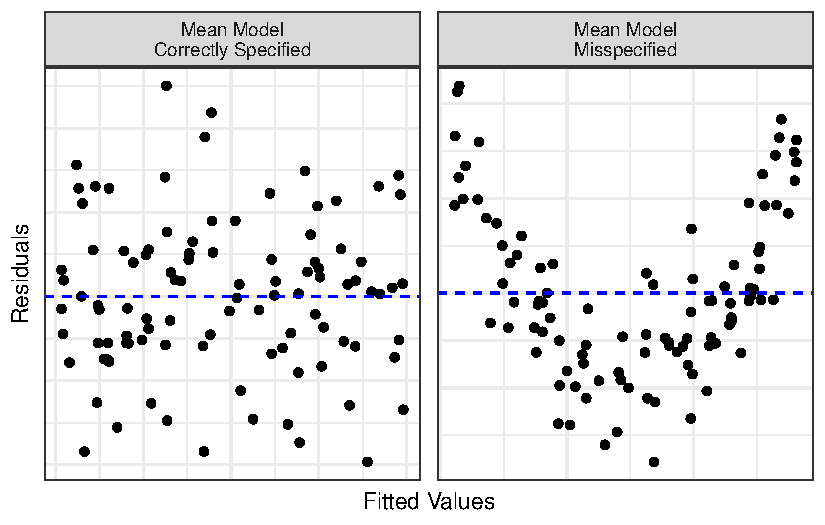
\includegraphics[width=0.8\textwidth,height=\textheight]{./images/fig-residual-plot-1.pdf}

}

\caption{\label{fig-residual-plot}Plot of the residuals against the
fitted values for two hypothetical models. One illustrates what we would
expect under a correctly specified mean model; the second is an example
of a graphic indicating the mean model is misspecified.}

\end{figure}

\begin{tcolorbox}[enhanced jigsaw, leftrule=.75mm, coltitle=black, left=2mm, title=\textcolor{quarto-callout-note-color}{\faInfo}\hspace{0.5em}{Assessing Specification of Mean Response}, breakable, toptitle=1mm, bottomtitle=1mm, colback=white, colbacktitle=quarto-callout-note-color!10!white, titlerule=0mm, opacitybacktitle=0.6, colframe=quarto-callout-note-color-frame, bottomrule=.15mm, arc=.35mm, opacityback=0, rightrule=.15mm, toprule=.15mm]

If the mean response is correctly specified, we would expect the
residuals to balance around 0, regardless of the estimated mean
response. When examining a plot of the residuals against the fitted
values, any trends in the location suggest the functional form of the
mean response has been incorrectly specified.

\end{tcolorbox}

\begin{example}[Rehabilitation Therapy
Continued]\protect\hypertarget{exm-therapy-mean0}{}\label{exm-therapy-mean0}

Example~\ref{exm-therapy} described a study to investigate recovery time
among patients who have undergone a corrective knee surgery. Suppose we
are willing to believe that the mean recovery time is linearly related
to the age of a patient. Combining the model for the likelihood
suggested in Example~\ref{exm-therapy-likelihood} and the advice on
default priors specified in Chapter~\ref{sec-reg-priors}, consider the
following model:

\[
\begin{aligned}
  (\text{Recovery Time})_i &\mid (\text{Age})_i, \boldsymbol{\beta} \stackrel{\text{Ind}}{\sim}Exp\left(\theta_i\right) \\
  \theta_i &= \beta_0 + \beta_1 (\text{Age})_i \\
  \beta_0 &\sim Unif(0, 25) \\
  \beta_1 &\sim Unif(0, 5).
\end{aligned}
\]

This model was fit using an MCMC algorithm with 3 chains; a burn-in of
2000 was applied to each of the chains, and a total of 5000 samples were
generated for each chain (for a total of 9000 variates after the burn-in
period). The posterior mean was used to estimate each of the unknown
parameters. Figure~\ref{fig-mean0} presents the plot of the residuals
against the fitted values for this model. Comment on the assumption that
the mean response is properly specified.

\end{example}

\begin{figure}

{\centering 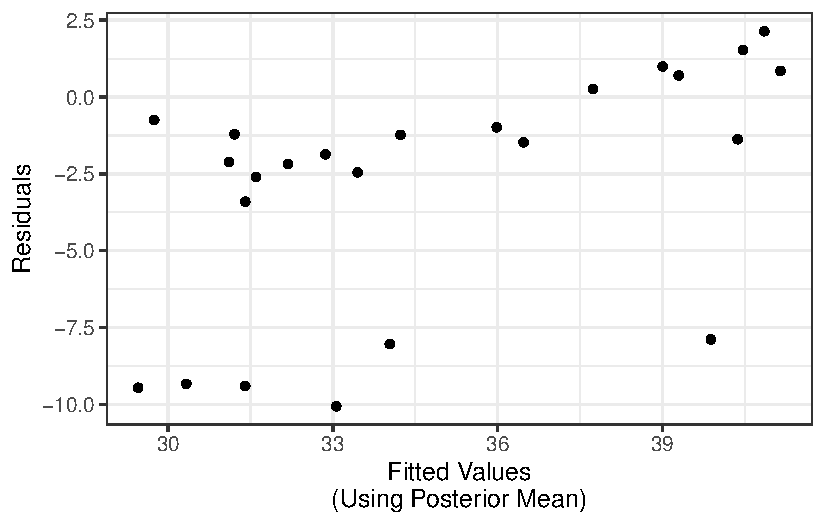
\includegraphics[width=0.8\textwidth,height=\textheight]{./images/fig-mean0-1.pdf}

}

\caption{\label{fig-mean0}Assessment of the mean response model for the
Therapy example.}

\end{figure}

\begin{solution}

If the mean response model is correctly specified, we would expect the
residuals to balance around 0 for all fitted values. Notice that the
residuals are centered below for the majority of the graphic, and only
balance around 0 for large fitted values. This trend in the location of
the residuals suggests the mean response model was not correct
specified.

In particular, this slight upward trend suggests that perhaps we were
incorrect in forcing the intercept to be positive (remember, our prior
distribution forced the support for the intercept to be positive). We
had done this because the mean response for an exponential distribution
must always be positive. However, because of extrapolation, forcing this
to be the case at an age of 0 seems to be problematic. There are two
approaches we could consider in addressing this:

\begin{itemize}
\tightlist
\item
  We could consider a different prior that allows the intercept to be
  negative, accepting that it is nonsensical and that the model will not
  predict well for small values of age.
\item
  We could center the age variable (by subtracting the average observed
  age from each observation). Center the age variable does not impact
  the slope, but it changes the interpretation of the intercept. In
  particular, the intercept would represent the average recovery time
  for a patient of average age. This avoids the problem of extrapolation
  when interpreting the intercept and might address the problems we are
  seeing above.
\end{itemize}

\end{solution}

The other primary assumption that we make when fitting a regression
model is that the conditional distribution of the response is
appropriate. In Example~\ref{exm-therapy-mean0}, for example, we are
assuming that the Exponential distribution for the response (conditional
on the age) is appropriate, as opposed to a Normal distribution, for
example. One technique for assessing whether this distributional
assumption is appropriate is to compare the posterior predictive
distribution with the observed distribution. As we have seen, the
posterior predictive distribution
(Definition~\ref{def-posterior-predictive-distribution}) can be
challenging to derive; fortunately, it is easily simulated using a
sample from the posterior distribution. With the general model of
Equation~\ref{eq-reg-meanmodel} in mind, we can generate the posterior
predictive distribution as follows:

\begin{itemize}
\tightlist
\item
  Obtain a sample of size \(M\) from the posterior distribution of each
  unknown parameter:
  \(\boldsymbol{\beta}^{(1)}, \boldsymbol{\beta}^{(2)}, \dotsc, \boldsymbol{\beta}^{(M)}\)
  and
  \(\boldsymbol{\theta}^{(1)}, \boldsymbol{\theta}^{(2)}, \dotsc, \boldsymbol{\theta}^{(M)}\).
\item
  For each sample from the posterior, generate a new \emph{sample} of
  \(n\) responses according to
  \((\text{Predicted Response})_i^{(m)} \sim f\left(\mu_i^{(m)}, \boldsymbol{\theta}^{(m)}\right)\)
  for \(m = 1, 2, \dotsc, M\). If we are conditioning on the predictors,
  they are taken to be those from the original sample.
\end{itemize}

The above two steps produces \(M\) new samples; each generated sample
will produce a unique distribution of the responses across the \(n\)
observations. We can summarize each of these \(M\) distributions using a
density plot, overlaid on the same graphic. Then, we can overlay the
density from the observed response to get a sense of how they compare.
Figure~\ref{fig-posterior-predictive-check} gives an example of what
this plot might look like.

\begin{tcolorbox}[enhanced jigsaw, leftrule=.75mm, coltitle=black, left=2mm, title=\textcolor{quarto-callout-note-color}{\faInfo}\hspace{0.5em}{Note}, breakable, toptitle=1mm, bottomtitle=1mm, colback=white, colbacktitle=quarto-callout-note-color!10!white, titlerule=0mm, opacitybacktitle=0.6, colframe=quarto-callout-note-color-frame, bottomrule=.15mm, arc=.35mm, opacityback=0, rightrule=.15mm, toprule=.15mm]

Due to the computational intensity of this graphic, it is common to do
this for a random sample of variates instead of all \(M\) variates
generated by the MCMC algorithm.

\end{tcolorbox}

\begin{tcolorbox}[enhanced jigsaw, leftrule=.75mm, coltitle=black, left=2mm, title=\textcolor{quarto-callout-warning-color}{\faExclamationTriangle}\hspace{0.5em}{Warning}, breakable, toptitle=1mm, bottomtitle=1mm, colback=white, colbacktitle=quarto-callout-warning-color!10!white, titlerule=0mm, opacitybacktitle=0.6, colframe=quarto-callout-warning-color-frame, bottomrule=.15mm, arc=.35mm, opacityback=0, rightrule=.15mm, toprule=.15mm]

It is important to remember that comparing the posterior predictive
distribution to that of the observed distribution is combining multiple
conditions/assumptions together: the complete form of the distribution
as well as how the individual observations vary compared to how the
aggregate dataset varies. While our modeling is conditioned, the density
of the observed response marginalizes across the predictors. Care must
be taken not to over-interpret this graphic as proving we have the
correct model.

\end{tcolorbox}

\begin{figure}

{\centering 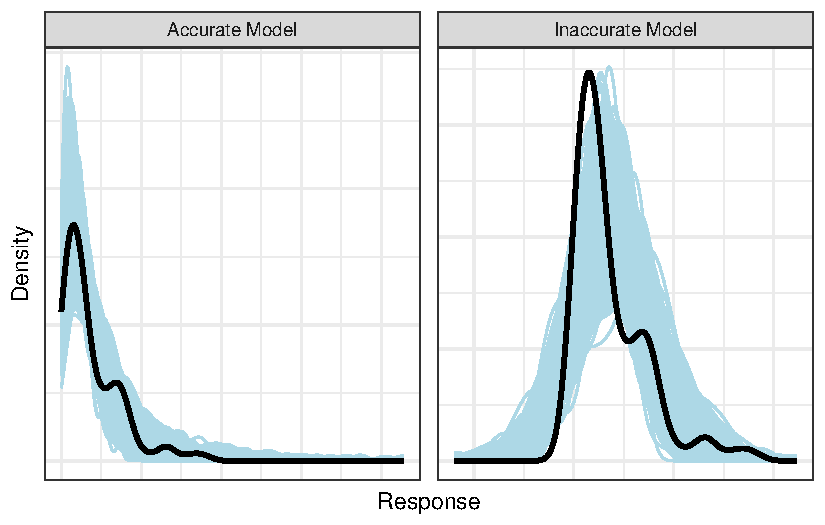
\includegraphics[width=0.8\textwidth,height=\textheight]{./images/fig-posterior-predictive-check-1.pdf}

}

\caption{\label{fig-posterior-predictive-check}Two plots of the
posterior predictive distributions from a regression model with the
observed distribution. One illustrates what we would expect when the
distribution accurately captures the process; the second is an example
of a graphic indicating the distributional assumptions are incorrect.}

\end{figure}

\begin{tcolorbox}[enhanced jigsaw, leftrule=.75mm, coltitle=black, left=2mm, title=\textcolor{quarto-callout-note-color}{\faInfo}\hspace{0.5em}{Assessing the Likelihood}, breakable, toptitle=1mm, bottomtitle=1mm, colback=white, colbacktitle=quarto-callout-note-color!10!white, titlerule=0mm, opacitybacktitle=0.6, colframe=quarto-callout-note-color-frame, bottomrule=.15mm, arc=.35mm, opacityback=0, rightrule=.15mm, toprule=.15mm]

If the model for the likelihood is correctly specified, then the
marginal distribution of the observed response should be similar to the
posterior predictive distribution given the observed data. For a
regression model, this is done by generating several \emph{samples} of
the same size given the posterior variates; if the distributional model
is appropriate, a density plot of the observed response should line up
with the density plots of those samples generated from the posterior
variates. Any major differences in these shapes would suggest
\emph{some} aspect of the model (including the distributional form) is
incorrect.

\end{tcolorbox}

\begin{example}[Rehabilitation Therapy
Continued]\protect\hypertarget{exm-therapy-postpred}{}\label{exm-therapy-postpred}

Example~\ref{exm-therapy-mean0} presented a model for the study
described in Example~\ref{exm-therapy}. Figure~\ref{fig-postpredcond} is
a plot of the posterior predicted distribution of the responses (using
250 randomly selected posterior variates) against the observed
distribution of the response. Comment on the assumption that the
distributional model specified is appropriate.

\end{example}

\begin{figure}

{\centering 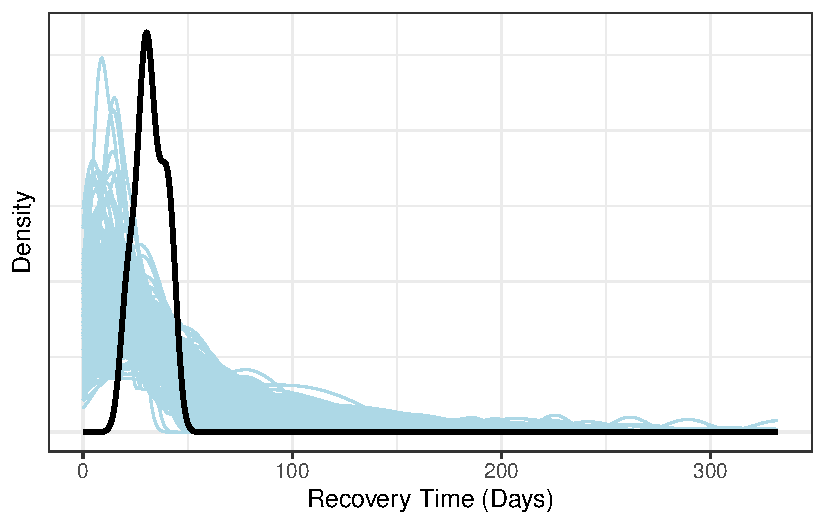
\includegraphics[width=0.8\textwidth,height=\textheight]{./images/fig-postpredcond-1.pdf}

}

\caption{\label{fig-postpredcond}Assessment of the distributional
assumptions for the Therapy example.}

\end{figure}

\begin{solution}

The observed marginal distribution of the response is very different
than the predicted distributions. While this could be due in part to the
misspecification of the mean response model (as noted in
Example~\ref{exm-therapy-mean0}), the level of departure here suggests
the distributional assumption on the likelihood is also incorrect. If we
wanted to be sure, we should refit the model using a different mean
response function first, and then repeat this process.

\end{solution}

\hypertarget{sec-discrete-responses}{%
\chapter{Regression Models for Categorical
Responses}\label{sec-discrete-responses}}

\providecommand{\norm}[1]{\lVert#1\rVert}
\providecommand{\abs}[1]{\lvert#1\rvert}
\providecommand{\iid}{\stackrel{\text{IID}}{\sim}}
\providecommand{\ind}{\stackrel{\text{Ind}}{\sim}}

\providecommand{\bm}[1]{\mathbf{#1}}
\providecommand{\bs}[1]{\boldsymbol{#1}}
\providecommand{\bbeta}{\bs{\beta}}

\providecommand{\Ell}{\mathcal{L}}
\providecommand{\indep}{\perp\negthickspace\negmedspace\perp}

On the one hand, modeling a categorical response (where the response
follows a discrete distribution) is no different than modeling a
quantitative response (where the response follows a continuous
distribution). In both cases, we specify a distribution, and we allow
one or more parameters to vary across individuals based on their
predictors through some pre-specified function. On the other hand, the
modeling is quite different as there are often more pitfalls to be aware
of. In particular, we are no longer in a position to think of the model
as

\[(\text{Response})_i = (\text{Signal})_i + (\text{Noise})_i.\]

As an example, if the response is binary, what type of noise could be
added to ``jitter'' the response? A binary response must always take the
value 0 or 1, which implies that thinking of the response as a
``jittered'' signal seems somehow inauthentic. The key to extending the
regression model to categorical response variables is to view regression
as an extension as a more complex specification of the conditional
response.

\hypertarget{considerations-for-a-binary-response}{%
\section{Considerations for a Binary
Response}\label{considerations-for-a-binary-response}}

Suppose our response is binary, taking the value 1 when an event of
interest occurs (a ``success'') and taking the value 0 when the event
does not occur (a ``failure''). A starting point for this model is

\[(\text{Response})_i \stackrel{\text{Ind}}{\sim}Ber\left(\theta_i\right),\]

where we are allowing the probability of success \(\theta_i\) to
potentially vary from one observation to the next. This model continues
to assume the response from one individual is independent of the
response from any other individual. Our initial attempt at generalizing
to a regression setting may be to borrow the linear model structure of
the previous chapters and consider

\[\theta_i = \beta_0 + \sum_{j=1}^{p} \beta_j (\text{Predictor } j)_i.\]

Unfortunately, this can be a poor strategy. Notice that there is nothing
ensuring that this linear function produces values of \(\theta_i\) which
are consistent with its support (this is the same problem we encountered
in Example~\ref{exm-therapy-likelihood}). That is, we know that since
\(\theta_i\) is a probability, its support is the interval \((0, 1)\).
The linear function, however, could quite easily produce values which
are negative or exceed 1; instead, we desire a function that is always
bounded between 0 and 1, similar to that represented in
Figure~\ref{fig-logistic-regression}.

\begin{figure}

{\centering 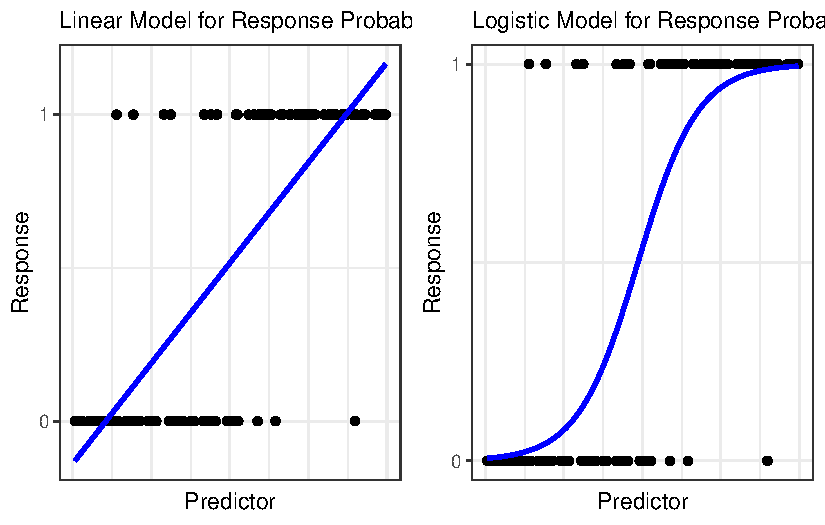
\includegraphics[width=0.8\textwidth,height=\textheight]{./images/fig-logistic-regression-1.pdf}

}

\caption{\label{fig-logistic-regression}Comparison of two functional
forms of a single predictor for the success probability in a regression
for a binary response. The first indicates the problems with a linear
functional form, while the second illustrates a function that is bounded
on the correct support.}

\end{figure}

One of the most common choices for the functional form is the
\emph{logistic function}.

\begin{definition}[Logistic
Regression]\protect\hypertarget{def-logistic-regression}{}\label{def-logistic-regression}

Given a binary response; logistic regression assumes that

\[
\begin{aligned}
  (\text{Response})_i &\mid (\text{Predictors})_i, \boldsymbol{\beta} \stackrel{\text{Ind}}{\sim}Ber\left(\theta_i\right) \\
  \theta_i &= \frac{e^{\beta_0 + \sum_{j=1}^{p} \beta_j (\text{Predictor } j)_i}}{1 + e^{\beta_0 + \sum_{j=1}^{p} \beta_j (\text{Predictor } j)_i}}.
\end{aligned}
\]

\end{definition}

This is known as logistic regression because the functional form of the
probability matches that of the CDF of the Standard Logistic
Distribution:

\[\frac{e^x}{1+e^{x}}.\]

\begin{tcolorbox}[enhanced jigsaw, leftrule=.75mm, coltitle=black, left=2mm, title=\textcolor{quarto-callout-note-color}{\faInfo}\hspace{0.5em}{Note}, breakable, toptitle=1mm, bottomtitle=1mm, colback=white, colbacktitle=quarto-callout-note-color!10!white, titlerule=0mm, opacitybacktitle=0.6, colframe=quarto-callout-note-color-frame, bottomrule=.15mm, arc=.35mm, opacityback=0, rightrule=.15mm, toprule=.15mm]

When performing regression with a binary response, any CDF could be used
for the functional form relating the predictors to the success
probability; however, the Standard Logistic (``logistic regression'')
and Standard Normal (``probit regression'') distributions are most
common.

\end{tcolorbox}

Using a CDF for the functional form ensures that for any choice of
\(\boldsymbol{\beta}\) and the predictors, the function will always take
a value between 0 and 1. Notice that our choice of \(\theta_i\) is
\emph{nonlinear} in the parameters \(\boldsymbol{\beta}\); however, it
still has that feel of a linear model because of the \emph{linear
predictor}

\[\beta_0 + \sum_{j=1}^{p} \beta_j (\text{Predictor } j)_i.\]

Nothing prohibits us from considering a nonlinear function instead of
the linear predictor; it is just common practice to use the linear
predictor, as we have already seen it is flexible enough to accommodate
categorical predictors and curvature.

For a logistic regression, the \(j\)-th coefficient \(\beta_j\) is the
log odds ratio of the response occurring when the \(j\)-th predictor is
increased by one unit compared to its current value, holding all other
predictors fixed. For probit regression, the \(j\)-th coefficient
\(\beta_j\) has no intuitive interpretation (hence the popularity of
logistic regression).

\hypertarget{considerations-for-count-data}{%
\section{Considerations for Count
Data}\label{considerations-for-count-data}}

As in the binary response setting, we take care to ensure that the
functional form relating the predictors to key parameters in the
conditional distribution of the response enforces constraints on the
support.

Consider a response which counts the number of successes out of a fixed
number of trials. We might consider a model of the form

\[
\begin{aligned}
  (\text{Response})_i &\mid (\text{Predictors})_i, \boldsymbol{\beta} \stackrel{\text{Ind}}{\sim}Bin\left(m_i, \theta_i\right) \\
\log\left(\frac{\theta_i}{1-\theta_i}\right) &= \beta_0 + \sum_{j=1}^{p} \beta_j (\text{Predictor } j)_i.
\end{aligned}
\]

While we have written this in a slightly different form, we are using
the same functional form for linking the response probability to the
predictors; here, we have written it in terms of the \emph{link
function}.

\begin{definition}[Link
Function]\protect\hypertarget{def-link-function}{}\label{def-link-function}

The functional form ``linking'' the linear predictor

\[\beta_0 + \sum_{j=1}^{p} \beta_j (\text{Predictor } j)_i\]

to the mean response of the model in a regression model. In particular,
it is the function \(g\) such that

\[g\left(\theta_i\right) = \beta_0 + \sum_{j=1}^{p} \beta_j (\text{Predictor } j)_i.\]

Common link functions include:

\begin{itemize}
\tightlist
\item
  Identity link: \(g\left(\theta_i\right) = \theta_i\)
\item
  Logit link:
  \(g\left(\theta_i\right) = \log\left(\frac{\theta_i}{1 - \theta_i}\right)\)
\item
  Log link: \(g\left(\theta_i\right) = \log\left(\theta_i\right)\)
\item
  Inverse link: \(g\left(\theta_i\right) = \frac{1}{\theta_i}\)
\item
  Negative inverse link:
  \(g\left(\theta_i\right) = -\frac{1}{\theta_i}\)
\item
  Inverse squared link:
  \(g\left(\theta_i\right) = \frac{1}{\theta_i^2}\)
\end{itemize}

\end{definition}

The logistic distribution function is chosen since \(\theta_i\) should
be constrained to the interval \((0, 1)\). Notice that using the logit
link for the success probability in the Binomial distribution on the
response does not specify the mean response directly; instead, it is
simply used to link the predictors to the mean response such that

\[E\left[(\text{Response}) \mid (\text{Predictors}), \boldsymbol{\beta}\right] = m  \frac{e^{\beta_0 + \sum_{j=1}^{p} \beta_j (\text{Predictor } j)}}{1 + e^{\beta_0 + \sum_{j=1}^{p} \beta_j (\text{Predictor } j)}},\]

where \(m\) is the number of trials.

\begin{tcolorbox}[enhanced jigsaw, leftrule=.75mm, coltitle=black, left=2mm, title=\textcolor{quarto-callout-note-color}{\faInfo}\hspace{0.5em}{Note}, breakable, toptitle=1mm, bottomtitle=1mm, colback=white, colbacktitle=quarto-callout-note-color!10!white, titlerule=0mm, opacitybacktitle=0.6, colframe=quarto-callout-note-color-frame, bottomrule=.15mm, arc=.35mm, opacityback=0, rightrule=.15mm, toprule=.15mm]

Any distribution for which the mean response is defined through the
``success'' probability (Bernoulli, Binomial, Geometric) could
potentially make use of the logit link.

\end{tcolorbox}

The Poisson distribution is common for modeling the number of rare
events in a large population, or for arbitrary counts that have no upper
bound. Extending this into a regression model generally takes the form

\[
\begin{aligned}
  (\text{Response})_i &\mid (\text{Predictors})_i, \boldsymbol{\beta} \stackrel{\text{Ind}}{\sim}Poisson\left(\lambda_i\right) \\
  \log\left(\lambda_i\right) &= \beta_0 + \sum_{j=1}^{p} \beta_j (\text{Predictor } j)_i.
\end{aligned}
\]

The log link function is chosen to ensure that \(\lambda > 0\) for all
possible choices of the parameter vector \(\boldsymbol{\beta}\) and
predictors.

In each of the cases considered in this chapter, the model specifies the
mean response; however, it also specifies the variability in the
response. For example, the mean of a Poisson distribution is
\(\lambda_i\), and the variance is also given by \(\lambda_i\). These
distributional models are unique in that knowing the mean response
uniquely determines the variability in the response. Occasionally, we
come across data for which the response behaves \emph{nearly} like one
of these distributions; however, additional variability is present.
There are ways of generalizing these models to account for this
additional dispersion.

\bookmarksetup{startatroot}

\hypertarget{references}{%
\chapter*{References}\label{references}}
\addcontentsline{toc}{chapter}{References}

\markboth{References}{References}

\hypertarget{refs}{}
\begin{CSLReferences}{1}{0}
\leavevmode\vadjust pre{\hypertarget{ref-Doyle1890}{}}%
Doyle, Sir Arthur Conan. 1890. \emph{The Sign of the Four}. Spencer
Blackett.

\leavevmode\vadjust pre{\hypertarget{ref-Dudeck1981}{}}%
Dudeck, A E, and C H Peeacock. 1981. {``Effects of Several Overseeded
Ryegrasses on Turf Quality, Traffic Tolerance and Ball Roll.''} In
\emph{Proceedings of the Fourth International Turfgrass Research
Conference}, edited by R W Sheard, 75--81.

\leavevmode\vadjust pre{\hypertarget{ref-Goldstein2011}{}}%
Goldstein, Bernard D, Howard J Osofsky, and Maureen Y Lichtveld. 2011.
{``The Gulf Oil Spill.''} \emph{The New England Journal of Medicine}
364: 1334--48. \url{https://doi.org/10.1056/NEJMra1007197}.

\leavevmode\vadjust pre{\hypertarget{ref-Johnson2003}{}}%
Johnson, Eric J, and Daniel Goldstein. 2003. {``Do Defaults Save
Lives?''} \emph{Science} 302: 1338--39.

\leavevmode\vadjust pre{\hypertarget{ref-Kruschke2015}{}}%
Kruschke, John K. 2015. \emph{Doing Bayesian Data Analysis: A Tutorial
with r, JAGS, and Stan}. 2nd ed. Elsevier.

\leavevmode\vadjust pre{\hypertarget{ref-Lee1992}{}}%
Lee, J. 1992. {``Relationships Between Properties of Pulp-Fibre and
Paper.''}

\leavevmode\vadjust pre{\hypertarget{ref-Tintle2015}{}}%
Tintle, Nathan, Beth L Chance, A J Rossman, S Roy, T Swanson, and J
VanderStoep. 2015. \emph{Introduction to Statistical Investigations}.
Wiley.

\end{CSLReferences}

\cleardoublepage
\phantomsection
\addcontentsline{toc}{part}{Appendices}
\appendix

\hypertarget{glossary}{%
\chapter{Glossary}\label{glossary}}

\providecommand{\norm}[1]{\lVert#1\rVert}
\providecommand{\abs}[1]{\lvert#1\rvert}
\providecommand{\iid}{\stackrel{\text{IID}}{\sim}}
\providecommand{\ind}{\stackrel{\text{Ind}}{\sim}}

\providecommand{\bm}[1]{\mathbf{#1}}
\providecommand{\bs}[1]{\boldsymbol{#1}}
\providecommand{\bbeta}{\bs{\beta}}

\providecommand{\Ell}{\mathcal{L}}
\providecommand{\indep}{\perp\negthickspace\negmedspace\perp}

The following key terms were defined in the text; each term is presented
with a link to where the term was first encountered in the text.

\begin{description}
\tightlist
\item[Alternative Hypothesis
(Definition~\ref{def-alternative-hypothesis})]
The statement (or theory) about the parameter capturing what we would
like to provide evidence \emph{for}; this is the opposite of the null
hypothesis. This is denoted \(H_1\) or \(H_a\), read ``H-one'' and
``H-A'' respectively.
\item[Average (Definition~\ref{def-average})]
Also known as the ``mean,'' this measure of location represents the
balance point for the distribution. If \(x_i\) represents the \(i\)-th
value of the variable \(x\) in the sample, the sample mean is typically
denoted by \(\bar{x}\).
\end{description}

For a sample of size \(n\), it is computed by
\[\bar{x} = \frac{1}{n}\sum_{i=1}^{n} x_i.\]

When referencing the average for a population, the mean is also called
the ``Expected Value,'' and is often denoted by \(\mu\).

\begin{description}
\tightlist
\item[Axioms of Probability (Definition~\ref{def-axioms})]
Let \(\mathcal{S}\) be the sample space of a random process. Suppose
that to each event \(A\) within \(\mathcal{S}\), a number denoted by
\(Pr(A)\) is associated with \(A\). If the map \(Pr(\cdot)\) satisfies
the following three axioms, then it is called a \textbf{probability}:
\end{description}

\begin{enumerate}
\def\labelenumi{\arabic{enumi}.}
\tightlist
\item
  \(Pr(A) \geq 0\)
\item
  \(Pr(\mathcal{S}) = 1\)
\item
  If \(\left\{A_1, A_2, \dotsc\right\}\) is a sequence of mutually
  exclusive events in \(\mathcal{S}\), then
\end{enumerate}

\[Pr\left(\bigcup_{i = 1}^{\infty} A_i\right) = \sum_{i = 1}^{\infty} Pr\left(A_i\right).\]

\(Pr(A)\) is said to be the ``probability of \(A\)'' or the
``probability \(A\) occurs.''

\begin{description}
\tightlist
\item[Bayes Factor (Definition~\ref{def-bayes-factor})]
A measure of how the observed data \emph{alters} your prior beliefs
about a hypothesis. Let \(H_j\) denote the hypothesis that
\(\theta \in \Theta_j\) for some region \(\Theta_j\). The Bayes Factor
\emph{in favor of} \(H_j\) is the ratio of the posterior odds in favor
of \(H_j\) to the prior odds in favor of \(H_j\):
\end{description}

\[BF_j = \left(\frac{Pr\left(\theta \in \Theta_j \mid \mathbf{y}\right)}{Pr\left(\theta \notin \Theta_j \mid \mathbf{y}\right)}\right)\left(\frac{Pr\left(\theta \notin \Theta_j\right)}{Pr\left(\theta \in \Theta_j\right)}\right).\]

\begin{description}
\tightlist
\item[Bayes Factor for Model Comparison
(Definition~\ref{def-bayes-factor-models})]
The Bayes Factor, in favor of Model 1, is
\end{description}

\[
\begin{aligned}
  BF_{1} &= \left(\frac{Pr(\mathcal{M}_1 \mid \mathbf{y})}{Pr(\mathcal{M}_0 \mid \mathbf{y})}\right)\left(\frac{Pr(\mathcal{M}_0)}{Pr(\mathcal{M}_1)}\right) \\
    &= \left(\frac{f_1(\mathbf{y} \mid \mathcal{M}_1) Pr(\mathcal{M}_1)}{f_0(\mathbf{y} \mid \mathcal{M}_0) Pr(\mathcal{M}_0)}\right)\left(\frac{Pr(\mathcal{M}_0)}{Pr(\mathcal{M}_1)}\right) \\
    &= \frac{f_1(\mathbf{y} \mid \mathcal{M}_1)}{f_0(\mathbf{y} \mid \mathcal{M}_0)}.
\end{aligned}
\]

That is, the Bayes Factor is a ratio of the evidence for each model.

\begin{description}
\tightlist
\item[Bias (Definition~\ref{def-bias})]
A set of measurements is said to be biased if they are
\emph{consistently} too high (or too low). Similarly, an estimate of a
parameter is said to be biased if it is \emph{consistently} too high (or
too low).
\item[Blocking (Definition~\ref{def-blocking})]
Blocking is a way of minimizing the variability contributed by an
inherent characteristic that results in dependent observations. In some
cases, the blocks are the unit of observation which is sampled from a
larger population, and multiple observations are taken on each unit. In
other cases, the blocks are formed by grouping the units of observations
according to an inherent characteristic; in these cases that shared
characteristic can be thought of having a value that was sampled from a
larger population.
\end{description}

In both cases, the observed blocks can be thought of as a random sample;
within each block, we have multiple observations, and the observations
from the same block are more similar than observations from different
blocks.

\begin{description}
\tightlist
\item[Bridge Sampling (Definition~\ref{def-bridge-sampling})]
The bridge sampling estimator of the marginal likelihood
\(m(\mathbf{y})\) is given by
\end{description}

\[
\begin{aligned}
  m(\mathbf{y}) 
    &= \int f(\mathbf{y} \mid \boldsymbol{\theta}) \pi(\boldsymbol{\theta}) d\boldsymbol{\theta} \\
    &= \frac{E_g\left[h(\boldsymbol{\theta}) f(\mathbf{y} \mid \boldsymbol{\theta}) \pi(\boldsymbol{\theta})\right]}{E_{\pi}\left[h(\boldsymbol{\theta}) g(\boldsymbol{\theta}) \right]} \\
    &\approx \frac{m^{-1}\sum_{j=1}^{m} h\left(\tilde{\boldsymbol{\theta}}_j\right) f\left(\mathbf{y} \mid \tilde{\boldsymbol{\theta}}_j\right) \pi\left(\tilde{\boldsymbol{\theta}}_j\right)}{m^{-1}\sum_{i=1}^{m} h\left(\boldsymbol{\theta}^*_j\right) g\left(\boldsymbol{\theta}^*_j\right)}
\end{aligned}
\]

where \(h(\boldsymbol{\theta})\) is called the bridge function and
\(g(\boldsymbol{\theta})\) is the proposal distribution. Here,
\(\tilde{\boldsymbol{\theta}}\) denotes a random variate from the
proposal distribution and \(\boldsymbol{\theta}^*\) a random variate
from the posterior; \(E_g\) denotes taking an expectation with respect
to the proposal distribution and \(E_\pi\) denotes taking an expectation
with respect to the posterior distribution.

\begin{description}
\tightlist
\item[Categorical Variable (Definition~\ref{def-categorical})]
Also called a ``qualitative variable,'' a measurement on a subject which
denotes a grouping or categorization.
\item[Codebook (Definition~\ref{def-codebook})]
Also called a ``data dictionary,'' these provide complete information
regarding the variables contained within a dataset.
\item[Conditional Density (Definition~\ref{def-conditional-density})]
Let \(X\) and \(Y\) be two random variables; the conditional density of
\(X\) given \(Y\) is
\end{description}

\[f_{X \mid Y}(y \mid x) = \frac{f_{X, Y}(x, y)}{f_Y(y)}\]

\begin{description}
\tightlist
\item[Conditional Density (Definition~\ref{def-conditional-density})]
Let \(\mathbf{X}\) be a random vector; without loss of generality,
partition \(\mathbf{X}\) such that
\end{description}

\[\mathbf{X} = \begin{pmatrix} \mathbf{X}_1 \\ \mathbf{X}_2 \end{pmatrix}\]

where \(\mathbf{X}_1\) represents the first \(k\) components and
\(\mathbf{X}_2\) represents the remaining \(n-k\) components. Then, the
conditional density of \(\mathbf{X}_1\) given \(\mathbf{X}_2\) is

\[f_{\mathbf{X}_1 \mid \mathbf{X}_2}(\mathbf{x}_1 \mid \mathbf{x}_2) = \frac{f_{\mathbf{X}}(\mathbf{x})}{f_{\mathbf{X}_2}(\mathbf{x}_2)}.\]

\begin{description}
\tightlist
\item[Conditional Independence
(Definition~\ref{def-conditional-independence})]
Two random variables \(X\) and \(Y\) are said to be independent,
conditional on (or ``given'') \(Z\) if, and only if,
\end{description}

\[f_{(X,Y) \mid Z} (x, y \mid z) = f_{X \mid Z}(x \mid z) f_{Y \mid Z}(y \mid z).\]

\begin{description}
\tightlist
\item[Confounding (Definition~\ref{def-confounding})]
When the effect of a variable on the response is mis-represented due to
the presence of a third, potentially unobserved, variable known as a
confounder.
\item[Conjugate Prior (Definition~\ref{def-conjugate-prior})]
A prior distribution chosen such that the posterior distribution belongs
to the same family as the prior distribution, with the (hyper)parameters
that govern the family updated based on the observed data.
\item[Continuous and Discrete Random Variable
(Definition~\ref{def-rvtypes})]
The random variable \(X\) is said to be a discrete random variable if
its corresponding support is countable. The random variable \(X\) is
said to be a continuous random variable if the corresponding support is
uncountable (such as an interval or a union of intervals on the real
line).
\item[Controlled Experiment
(Definition~\ref{def-controlled-experiment})]
A study in which each subject is \emph{randomly} assigned to one of the
groups being compared in the study.
\item[Credible Interval (Definition~\ref{def-credible-interval})]
A \(100c\)\% credible interval is an interval \((a, b)\) such that
\end{description}

\[Pr(a \leq \theta \leq b \mid \mathbf{y}) = \int_{a}^{b} \pi(\theta \mid \mathbf{y})d\theta = c.\]

\begin{description}
\tightlist
\item[Cumulative Distribution Function (CDF) (Definition~\ref{def-cdf})]
Let \(X\) be a random variable; the cumulative distribution function
(CDF) is defined as
\end{description}

\[F(u) = Pr(X \leq u).\]

For a continuous random variable, we have that

\[F(u) = \int_{-\infty}^{u} f(x) dx\]

implying that the density function is the derivative of the CDF. For a
discrete random variable

\[F(u) = \sum_{x \leq u} f(x).\]

\begin{description}
\tightlist
\item[Density Function (Definition~\ref{def-density-function})]
A density function \(f\) relates the values in the support of a random
variable with the probability of observing those values.
\end{description}

Let \(X\) be a continuous random variable, then its density function
\(f\) is the function such that

\[Pr(a \leq X \leq b) = \int_a^b f(x) dx\]

for any real numbers \(a\) and \(b\) in the support.

Let \(X\) be a discrete random variable, then its density function \(f\)
is the function such that

\[Pr(X = u) = f(u)\]

for any real number \(u\) in the support.

\begin{description}
\tightlist
\item[Dirac Delta Function (Definition~\ref{def-dirac-delta})]
The Dirac delta function is the function (not in a rigorous sense)
\(\delta\) such that
\end{description}

\[\int_{-\infty}^{\infty} \delta(x) dx = 1\]

and

\[\int_{-\infty}^{\infty} f(x) \delta(x) dx = f(0)\]

for any real-valued function \(f\).

The Dirac delta function allows us to describe a discrete distribution,
which places mass at a single point, as a continuous function on the
real line.

\begin{description}
\tightlist
\item[Distribution (Definition~\ref{def-distribution})]
The pattern of variability corresponding to a set of values.
\item[Distribution of the Population
(Definition~\ref{def-distribution-population})]
The pattern of variability in values of a variable at the population
level. Generally, this is impossible to know, but we might model it.
\item[Distribution of the Sample
(Definition~\ref{def-distribution-sample})]
The pattern of variability in the observed values of a variable.
\item[Effective Sample Size (Definition~\ref{def-ess})]
The effective sample size (ESS) is given by
\end{description}

\[ESS = \frac{N}{1 + 2\sum_{k=1}^{\infty} ACF(k)}\]

where ACF is the auto-correlation function of degree \(k\).

\begin{description}
\tightlist
\item[Equal-Tailed Credible Interval
(Definition~\ref{def-equal-tail-interval})]
The equal-tailed credible interval, which is probably the most commonly
used in practice, chooses endpoints such that
\end{description}

\[Pr(\theta < a \mid \mathbf{y}) = \frac{1-c}{2} = Pr(\theta > b \mid \mathbf{y}).\]

\begin{description}
\tightlist
\item[Estimation (Definition~\ref{def-estimation})]
Using the sample to approximate the value of a parameter from the
underlying population.
\item[Event (Definition~\ref{def-event})]
A subset of the sample space that is of particular interest.
\item[Evidence for a Model (Definition~\ref{def-evidence})]
Under the Model Comparison framework defined above, the evidence for
model \(\mathcal{M}_j\) is defined as
\end{description}

\[f_j(\mathbf{y} \mid \mathcal{M}_j) = \int f_j(\mathbf{y} \mid \theta_j, \mathcal{M}_j) \pi_j(\theta_j \mid \mathcal{M}_j) d\theta_j.\]

\begin{description}
\tightlist
\item[Expectation of a Function (Definition~\ref{def-expectation})]
Let \(X\) be a random variable with density function \(f\) over the
support \(\mathcal{S}\), and let \(g\) be a real-valued function. Then,
\end{description}

\[E\left[g(X)\right] = \int_{\mathcal{S}} g(x) f(x) dx\]

for continuous random variables and

\[E\left[g(X)\right] = \sum_{\mathcal{S}} g(x) f(x)\]

for discrete random variables.

\begin{description}
\tightlist
\item[Expected Value (Mean) (Definition~\ref{def-mean})]
Let \(X\) be a random variable with density function \(f\) defined over
the support \(\mathcal{S}\). The expected value of a random variable,
also called the mean and denoted \(E(X)\), is given by
\end{description}

\[E(X) = \int_{\mathcal{S}} x f(x) dx\]

for continuous random variables and

\[E(X) = \sum_{\mathcal{S}} x f(x)\]

for discrete random variables.

\begin{description}
\tightlist
\item[Extrapolation (Definition~\ref{def-extrapolation})]
Extrapolation occurs when we use a model to predict outside of the
region for which data is available.
\item[Frequency (Definition~\ref{def-frequency})]
The number of observations in a sample falling into a particular group
(level) defined by a categorical variable.
\item[Frequentist Interpretation of Probability
(Definition~\ref{def-frequentist-interpretation})]
In this perspective, the probability of \(A\) describes the long-run
behavior of the event. Specifically, consider repeating the random
process \(m\) times, and let \(f(A)\) represent the number of times the
event \(A\) occurs out of those \(m\) replications. Then,
\end{description}

\[Pr(A) = \lim_{m \rightarrow \infty} \frac{f(A)}{m}.\]

\begin{description}
\tightlist
\item[General Mixture Distribution
(Definition~\ref{def-general-mixture-distribution})]
Let \(\theta\) be a parameter with support \(\Theta\), and let
\(\pi_k(\theta)\) be a valid distribution on the support, for
\(k = 1, 2, \dotsc, K\). Then,
\end{description}

\[\pi(\theta) = \sum_{k=1}^{K} w_k \pi_k(\theta)\]

is a valid prior distribution provided \(\sum_{k=1}^{K} w_k = 1\).

\begin{description}
\tightlist
\item[Highest Density Interval (Definition~\ref{def-hdi})]
The highest density interval, often called an HDI or HPD (for highest
posterior density), chooses the endpoints such that the interval is as
short as possible.
\end{description}

When the density is unimodal, this can be accomplished by choosing the
endpoints \(a\) and \(b\) such that

\[\pi(\theta \mid \mathbf{y}) \mid_{\theta = a} = \pi(\theta \mid \mathbf{y}) \mid_{\theta = b}\]

and

\[\int_{a}^{b} \pi(\theta \mid \mathbf{y} d\theta = c.\]

\begin{description}
\tightlist
\item[Histogram Approach to Constructing a Prior
(Definition~\ref{def-histogram-prior})]
Using expert information, attach probability to various intervals for
the parameter. Specifically,
\end{description}

\begin{itemize}
\tightlist
\item
  Define \(m\) intervals \(\left(\theta_{j-1}, \theta_j\right)\) for
  \(j = 1, 2, \dotsc, m\) that partition the parameter space; define
  \(\theta_0\) as the lower bound of the support for the parameter, and
  define \(\theta_m\) as the upper bound of the support for the
  parameter.
\item
  Eliciting expert opinions, assign probability \(\pi_j\) to each
  interval: \(\pi_j = Pr\left(\theta_{j-1} < \theta < \theta_j\right)\)
  for each \(j = 1, 2, \dotsc, m\).
\item
  Set the prior \(\pi(\theta)\) to be the piecewise distribution over
  this interval where \(\sum_{j=1}^{m} \pi_j = 1\).
\end{itemize}

\begin{description}
\tightlist
\item[Hyperparameter (Definition~\ref{def-hyperparameter})]
A constant term of a prior distribution that characterizes the family we
are considering.
\item[Hypothesis Testing (Definition~\ref{def-hypothesis-testing})]
Using a sample to determine if the data is consistent with a working
theory or if there is evidence to suggest the data is not consistent
with the theory.
\item[Identically Distributed
(Definition~\ref{def-identically-distributed})]
We say that random variables \(X\) and \(Y\) are identically distributed
if \(F_X(u) = F_Y(u)\) for all \(u\). This is equivalent to saying the
two random variables have the same density function \(f\).
\item[Independence (Definition~\ref{def-independence})]
Random variables \(X_1, X_2, \dotsc, X_n\) are said to be mutually
independent (or just ``independent'') if and only if
\end{description}

\[Pr\left(X_1 \in A_1, X_2 \in A_2, \dotsb, X_n \in A_n\right) = \prod_{i=1}^{n} Pr\left(X_i \in A_i\right),\]

where \(A_1, A_2, \dotsc, A_n\) are arbitrary sets. Perhaps more
helpful, \(X_1, X_2, \dotsc, X_n\) are said to be mutually independent
if and only if

\[f_{\mathbf{X}}(\mathbf{x}) = \prod_{i=1}^{n} f_{X_i}\left(x_i\right).\]

\begin{description}
\tightlist
\item[Indicator Variable (Definition~\ref{def-indicator-variable})]
An indicator variable is a binary variable (takes on the value 0 or 1),
taking the value 1 when a specific event occurs. A collection of \(k-1\)
indicator variables can be used to capture a categorical variable with
\(k\) levels in a regression model.
\end{description}

\begin{itemize}
\tightlist
\item
  The ``reference group'' (or reference level) is the group (level)
  defined by setting all indicator variables in a regression model to 0.
\end{itemize}

\begin{description}
\tightlist
\item[Interquartile Range (Definition~\ref{def-interquartile-range})]
Often abbreviated as IQR, this is the distance between the first and
third quartiles. This measure of spread indicates the range over which
the middle 50\% of the data is spread.
\item[Interval Estimation (Definition~\ref{def-interval-estimation})]
Interval estimation is the process of estimating a parameter with a
range of values. This is like trying to capture a target with a ring.
\item[Joint Density (Definition~\ref{def-joint-density})]
For a random vector \(\mathbf{X}\), the function
\(f_{\mathbf{X}}(\mathbf{x})\) such that for any set
\(A \in \mathbb{R}^n\), we have
\end{description}

\[Pr(\mathbf{X} \in A) = \int \dotsi \int_{A} f_{\mathbf{X}}(\mathbf{x}) dx_1 \dotsb dx_n\]

is called the joint density function; this is also referred to as the
\emph{likelihood}. Integrals are replaced by sums when appropriate.

\begin{description}
\tightlist
\item[Kernel of a Distribution (Definition~\ref{def-kernel})]
Let \(k(x)\) be a non-negative function of \(x\) over some region
\(\mathcal{S}_X\). Then, a valid density function \(f\) over the support
\(\mathcal{S}_X\) can be constructed by taking
\end{description}

\[f(x) = a k(x)\]

where \(a > 0\) is a suitably chosen scaling constant to ensure the
density integrates (or sums) to 1 over the support. The function \(k\)
is known as the kernel of the distribution, and it can be used to
identify the distributional family for a random variable.

\begin{description}
\tightlist
\item[Laplace Prior (Definition~\ref{def-laplace-prior})]
The Laplace prior, also known as a ``flat'' prior, considers the form
\end{description}

\[\pi(\theta) = 1 \qquad \forall \theta \in \Theta.\]

\begin{description}
\tightlist
\item[Link Function (Definition~\ref{def-link-function})]
The functional form ``linking'' the linear predictor
\end{description}

\[\beta_0 + \sum_{j=1}^{p} \beta_j (\text{Predictor } j)_i\]

to the mean response of the model in a regression model. In particular,
it is the function \(g\) such that

\[g\left(\theta_i\right) = \beta_0 + \sum_{j=1}^{p} \beta_j (\text{Predictor } j)_i.\]

Common link functions include:

\begin{itemize}
\tightlist
\item
  Identity link: \(g\left(\theta_i\right) = \theta_i\)
\item
  Logit link:
  \(g\left(\theta_i\right) = \log\left(\frac{\theta_i}{1 - \theta_i}\right)\)
\item
  Log link: \(g\left(\theta_i\right) = \log\left(\theta_i\right)\)
\item
  Inverse link: \(g\left(\theta_i\right) = \frac{1}{\theta_i}\)
\item
  Negative inverse link:
  \(g\left(\theta_i\right) = -\frac{1}{\theta_i}\)
\item
  Inverse squared link:
  \(g\left(\theta_i\right) = \frac{1}{\theta_i^2}\)
\end{itemize}

\begin{description}
\tightlist
\item[Logistic Regression (Definition~\ref{def-logistic-regression})]
Given a binary response; logistic regression assumes that
\end{description}

\[
\begin{aligned}
  (\text{Response})_i &\mid (\text{Predictors})_i, \boldsymbol{\beta} \stackrel{\text{Ind}}{\sim}Ber\left(\theta_i\right) \\
  \theta_i &= \frac{e^{\beta_0 + \sum_{j=1}^{p} \beta_j (\text{Predictor } j)_i}}{1 + e^{\beta_0 + \sum_{j=1}^{p} \beta_j (\text{Predictor } j)_i}}.
\end{aligned}
\]

\begin{description}
\tightlist
\item[Marginal Density (Definition~\ref{def-marginal-density})]
For a random vector \(\mathbf{X}\), the marginal density of the first
component \(X_1\) (without loss of generality) is
\end{description}

\[f_{X_1}(u) = \int \dotsi \int f_{\mathbf{X}}(\mathbf{x}) dx_2 \dotsb dx_n.\]

\begin{description}
\tightlist
\item[Markov Chain (Definition~\ref{def-markov-chain})]
A sequence of random vectors
\(\theta^{(0)}, \theta^{(1)}, \theta^{(2)}, \dotsc, \theta^{(n)}\) is a
Markov Chain with stationary transition probabilities if for any set
\(A\) and any \(k \leq n\)
\end{description}

\[
\begin{aligned}
  Pr\left(\theta^{(k)} \in A \mid \theta^{(1)}, \theta^{(2)}, \dotsc, \theta^{(k-1)}\right)
    &= Pr\left(\theta^{(k)} \in A \mid \theta^{(k-1)}\right) \\
    &= \int_{A} q\left(\theta^{(k)} \mid \theta^{(k-1)}\right) d\theta^{(k)}
\end{aligned}
\]

where \(q\) is called the transition kernel.

\begin{description}
\tightlist
\item[Method of Distribution Functions
(Definition~\ref{def-method-of-distribution-functions})]
Let \(X\) be a continuous random variable with density \(f\) and
cumulative distribution function \(F\). Consider \(Y = h(X)\). The
following process provides the density function \(g\) of \(Y\) by first
finding its cumulative distribution function \(G\).
\end{description}

\begin{enumerate}
\def\labelenumi{\arabic{enumi}.}
\tightlist
\item
  Find the set \(A\) for which \(h(X) \leq t\) if and only if
  \(X \in A\).
\item
  Recognize that
  \(G(y) = Pr(Y \leq y) = Pr\left(h(X) \leq y\right) = Pr(X \in A)\).
\item
  If interested in \(g(y)\), note that
  \(g(y) = \frac{\partial}{\partial y} G(y)\).
\end{enumerate}

\begin{description}
\tightlist
\item[Metropolis Algorithm (Definition~\ref{def-metropolis-algorithm})]
Suppose we want to generate random variates from the density
\(\pi(\theta \mid \mathbf{y})\). We perform the following steps:
\end{description}

\begin{enumerate}
\def\labelenumi{\arabic{enumi}.}
\tightlist
\item
  Generate an initial value \(\theta^{(0)}\).\\
\item
  At the \(k\)-th step, generate \(\theta^*\) (a candidate) according to
  a symmetric proposal density
  \(q\left(\theta \mid \theta^{(k-1)}\right)\).\\
\item
  Compute \(A\left(\theta^*, \theta^{(k-1)}\right)\) where
  \[A\left(\theta^*, \theta^{(k-1)}\right) = \frac{\pi\left(\theta^* \mid \mathbf{y}\right)}{\pi\left(\theta^{(k-1)} \mid \mathbf{y}\right)} = \frac{f\left(\mathbf{y} \mid \theta^*\right) \pi\left(\theta^*\right)}{f\left(\mathbf{y} \mid \theta^{(k-1)}\right) \pi\left(\theta^{(k-1)}\right)}.\]
\item
  Generate \(U \sim Unif(0,1)\). If
  \(U \leq A\left(\theta^*, \theta^{(k-1)}\right)\), then set
  \(\theta^{(k)} = \theta^*\); else, set
  \(\theta^{(k)} = \theta^{(k-1)}\).
\item
  Repeat Steps 2-4 \(m\) times, for some large \(m\).
\end{enumerate}

When generating an initial value, \(\theta^{(0)}\), we could choose
\(\theta^{(0)} \sim \pi(\theta)\) if the prior is easy to generate from.
While it is common to choose \(q(\cdot)\) to be a Normal distribution
with mean \(\theta^{(k-1)}\), it is not a requirement to do so; when a
Normal distribution is used, it can be difficult to determine a
reasonable variance (too large, and you drift too far away; too small,
and you do not move at all).

\begin{description}
\tightlist
\item[Mixture Distribution (Definition~\ref{def-mixture-distribution})]
Let \(X\) be a random variable and \(f(x)\) and \(g(x)\) be valid
density functions defined on a common support. Then,
\end{description}

\[h(x) = wf(x) + (1 - w) g(x),\]

where \(0 < w < 1\), is known as a mixture distribution.

\begin{description}
\tightlist
\item[Monte Carlo Error (Definition~\ref{def-mc-error})]
Also called the standard error for an approximation of the form
\(m^{-1} \sum\limits_{k=1}^{m} g\left(X_k\right)\), the MC error is
given by
\end{description}

\[\sqrt{\frac{1}{m(m-1)} \sum_{k=1}^{m} \left[g\left(X_k\right) - \frac{1}{m} \sum_{j=1}^{m} g\left(X_j\right)\right]^2}\]

which is the sample standard deviation of the generated variates divided
by the square root of the number of replications.

\begin{description}
\tightlist
\item[Monte Carlo Integration (Definition~\ref{def-mc-integration})]
Consider an integral of the form
\end{description}

\[\int_{\mathcal{S}} g(x) f(x) dx\]

where \(f(x)\) is a valid density function for a random variable \(X\)
with support \(\mathcal{S}\). Then, the following algorithm, known as
Monte Carlo (or MC) Integration, gives a numerical approximation to the
integral:

\begin{enumerate}
\def\labelenumi{\arabic{enumi}.}
\tightlist
\item
  Take a random sample \(X_1, X_2, \dotsc, X_m\) such that
  \(X_i \sim f(x)\) for all \(i\), where \(m\) is large.
\item
  Compute \(m^{-1} \sum_{i=1}^{m} g\left(X_i\right)\).
\end{enumerate}

By the Law of Large Numbers,

\[\frac{1}{m} \sum_{i=1}^{m} g\left(X_i\right) \approx \int_{\mathcal{S}} g(x) f(x) dx.\]

\begin{description}
\tightlist
\item[Noninformative Prior (Definition~\ref{def-noninformative-prior})]
A prior distribution which is derived solely based on the form of the
likelihood.
\item[Null Hypothesis (Definition~\ref{def-null-hypothesis})]
The statement (or theory) about the parameter that we would like to
\emph{disprove}. This is denoted \(H_0\), read ``H-naught'' or
``H-zero''.
\item[Null Value (Definition~\ref{def-null-value})]
The value associated with the equality component of the null hypothesis;
it forms the threshold or boundary between the hypotheses. Note: not all
questions of interest require a null value be specified.
\item[Numeric Variable (Definition~\ref{def-numeric})]
Also called a ``quantitative variable,'' a measurement on a subject
which takes on a numeric value \emph{and} for which ordinary arithmetic
makes sense.
\item[Observational Study (Definition~\ref{def-observational-study})]
A study in which each subject ``self-selects'' into one of groups being
compared in the study. The phrase ``self-selects'' is used very loosely
here and can include studies for which the groups are defined by an
inherent characteristic or are chosen haphazardly.
\item[Outlier (Definition~\ref{def-outlier})]
An individual observation which is so extreme, relative to the rest of
the observations in the sample, that it does not appear to conform to
the same distribution.
\item[Parameter (Definition~\ref{def-parameter})]
Numeric quantity which summarizes the distribution of a variable within
the \emph{population} of interest. Generally denoted by Greek letters in
statistical formulas.
\item[Percentile (Definition~\ref{def-percentile})]
The \(k\)-th percentile is the value \(q\) such that \(k\)\% of the
values in the distribution are less than or equal to \(q\). For example,
\end{description}

\begin{itemize}
\tightlist
\item
  25\% of values in a distribution are less than or equal to the 25-th
  percentile (known as the ``first quartile'' and denoted \(Q_1\)).
\item
  50\% of values in a distribution are less than or equal to the 50-th
  percentile (known as the ``median'').
\item
  75\% of values in a distribution are less than or equal to the 75-th
  percentile (known as the ``third quartile'' and denoted \(Q_3\)).
\end{itemize}

\begin{description}
\tightlist
\item[Percentile for a Random Variable
(Definition~\ref{def-population-percentile})]
Let \(X\) be a random variable with density function \(f\). The \(100k\)
percentile is the value \(q\) such that
\end{description}

\[Pr(X \leq q) = k.\]

\begin{description}
\tightlist
\item[Point Estimation (Definition~\ref{def-point-estimation})]
Point estimation is the process of estimating a parameter with a single
statistic. This is like trying to hit an infinitesimally small target
with a dart.
\item[Population (Definition~\ref{def-population})]
The collection of subjects we would like to say something about.
\item[Posterior Distribution
(Definition~\ref{def-posterior-distribution})]
A distribution quantifying our beliefs about the uncertainty in the
parameter(s) of the underlying sampling distribution \emph{after}
observing data. This is often denoted by
\(\pi(\boldsymbol{\theta} \mid \mathbf{y})\) where
\(\boldsymbol{\theta}\) is the parameter vector and \(\mathbf{y}\) the
observe data.
\end{description}

Given the likelihood \(f(\mathbf{y} \mid \boldsymbol{\theta})\) and a
prior distribution on the parameters \(\pi(\boldsymbol{\theta})\), the
posterior distribution is computed using Bayes Theorem:

\[\pi(\boldsymbol{\theta} \mid \mathbf{y}) = \frac{f(\mathbf{y} \mid \boldsymbol{\theta}) \pi(\theta)}{\int f(\mathbf{y} \mid \boldsymbol{\theta}) \pi(\boldsymbol{\theta}) d\boldsymbol{\theta}}.\]

\begin{description}
\tightlist
\item[Posterior Mean (Definition~\ref{def-posterior-mean})]
The posterior mean is the average value of the parameter, given the
data:
\end{description}

\[E\left[\boldsymbol{\theta} \mid \mathbf{y}\right] = \int \boldsymbol{\theta} \pi(\theta \mid \mathbf{y}) d\boldsymbol{\theta}.\]

\begin{description}
\tightlist
\item[Posterior Median (Definition~\ref{def-posterior-median})]
We are 50\% sure, given the data, the parameter falls below the
posterior median. Formally, the posterior median is the value \(q\) such
that
\end{description}

\[0.5 = \int_{-\infty}^{q} \pi(\theta \mid \mathbf{y}) d\theta.\]

\begin{description}
\tightlist
\item[Posterior Mode (Definition~\ref{def-posterior-mode})]
We think of the posterior mode as the most likely value of the
parameter, given the data. If the posterior distribution is continuous,
the posterior mode is the value of the parameter that maximizes the
posterior distribution. Formally, the posterior mode is given by
\end{description}

\[\arg \max_{\theta} \pi(\theta \mid \mathbf{y}).\]

\begin{description}
\tightlist
\item[Posterior Odds (Definition~\ref{def-posterior-odds})]
Let \(H_j\) denote the hypothesis that \(\theta \in \Theta_j\) for some
region \(\Theta_j\). Then, the posterior odds \emph{in favor of} \(H_j\)
is given by
\end{description}

\[\frac{Pr\left(\theta \in \Theta_j \mid \mathbf{y}\right)}{Pr\left(\theta \notin \Theta_j \mid \mathbf{y}\right)}.\]

\begin{description}
\tightlist
\item[Posterior Predictive Distribution
(Definition~\ref{def-posterior-predictive-distribution})]
Let \(\mathbf{Y}^*\) represent a collection of \(m\) \emph{future}
observations. The distribution of these future observations given the
observed data \(\mathbf{Y}\) (of length \(n\)), called the posterior
predictive distribution, is given by
\end{description}

\[\pi\left(\mathbf{y}^* \mid \mathbf{y}\right) = \int f\left(\mathbf{y}^* \mid \theta\right) \pi(\theta \mid \mathbf{y}) d\theta.\]

\begin{description}
\tightlist
\item[Potential (Definition~\ref{def-potential})]
The potential of a value \(\theta\) is the negative logarithm of the
posterior evaluated at \(\theta\). In practice, we need only know the
potential up to a constant. That is, it suffices to define the potential
as
\end{description}

\[\text{Potential}(\theta) = -\log\left[f(\mathbf{y} \mid \theta) \pi(\theta)\right].\]

\begin{description}
\tightlist
\item[Prior Distribution (Definition~\ref{def-prior-distribution})]
A distribution quantifying our beliefs about uncertainty in the
\emph{parameter(s)} of the underlying sampling distribution \emph{prior
to} observing any data. This is often denoted by
\(\pi(\boldsymbol{\theta})\) where \(\boldsymbol{\theta}\) is the
parameter vector.
\end{description}

\begin{itemize}
\tightlist
\item
  This relies on a \emph{subjective} view of probability.
\item
  As prior beliefs are subjective, there is no ``one'' prior, but each
  individual may have a unique prior.
\end{itemize}

\begin{description}
\tightlist
\item[Prior Predictive Distribution
(Definition~\ref{def-prior-predictive-distribution})]
The prior predictive distribution is the marginal distribution of the
response(s) prior to observing any data:
\end{description}

\[m(\mathbf{y}) = \int f(\mathbf{y} \mid \theta) \pi(\theta) d\theta.\]

The distribution marginalizes the parameter out of the likelihood using
the beliefs from the prior distribution.

\begin{description}
\tightlist
\item[Random Sample (Definition~\ref{def-random-sample})]
A random sample of size \(n\) refers to a collection of \(n\) random
variables \(X_1, X_2, \dotsc, X_n\) such that the random variables are
mutually independent, and the distribution of each random variable is
identical.
\item[Random Variable (Definition~\ref{def-random-variable})]
Let \(\mathcal{S}\) be the sample space corresponding to a random
process; a random variable \(X\) is a function mapping elements of the
sample space to the real line.
\end{description}

Random variables represent a measurement that will be collected during
the course of a study. Random variables are typically represented by a
capital letter.

\begin{description}
\tightlist
\item[Random Vector (Definition~\ref{def-random-vector})]
Let \(X_1, X_2, \dots, X_n\) be \(n\) random variables. Then, the vector
\(\mathbf{X} = \left(X_1, X_2, \dots, X_n\right)^\top\) is a random
vector of length \(n\).
\item[Randomization (Definition~\ref{def-randomization})]
Randomization can refer to random \emph{selection} or random
\emph{allocation}. Random selection refers to the use of a random
mechanism (e.g., a simple random sample,
Definition~\ref{def-simple-random-sample}, or a stratified random
sample, Definition~\ref{def-stratified-random-sample}) to select units
from the population. Random selection minimizes bias.
\end{description}

Random allocation refers to the use of a random mechanism when assigning
units to a specific treatment group in a controlled experiment
(Definition~\ref{def-controlled-experiment}). Random allocation
eliminates confounding and permits causal interpretations.

\begin{description}
\tightlist
\item[Reduction of Noise (Definition~\ref{def-noise-reduction})]
Reducing extraneous sources of variability can be accomplished by fixing
extraneous variables or blocking (Definition~\ref{def-blocking}). These
actions reduce the number of differences between the units under study.
\item[Regression (Definition~\ref{def-regression})]
A regression model is one for which the parameter(s) governing the data
generating process depends on one or more predictors. ``Parametric''
regression models do this through specifying a functional form for the
dependence of the parameter(s) on the predictor(s).
\item[Relative Frequency (Definition~\ref{def-relative-frequency})]
Also called the ``proportion,'' the fraction of observations falling
into a particular group (level) of a categorical variable.
\item[Replication (Definition~\ref{def-replication})]
Replication results from taking measurements on different units (or
subjects), for which you expect the results to be similar. That is, any
variability across the units is due to natural variability within the
population.
\item[Residual (Definition~\ref{def-residual})]
A residual is the difference between an observed response and the
predicted mean response for that same individual:
\end{description}

\[(\text{Residual})_i = (\text{Response})_i - (\text{Fitted Value})_i,\]

where

\[(\text{Fitted Value})_i = \widehat{\beta}_0 + \sum_{j=1}^{p} \widehat{\beta}_j (\text{Predictor} j)_i.\]

\begin{description}
\tightlist
\item[Response (Definition~\ref{def-response})]
The primary variable of interest within a study. This is the variable
you would either like to explain or estimate.
\item[Sample (Definition~\ref{def-sample})]
The collection of subjects for which we actually obtain measurements
(data).
\item[Sample Space (Definition~\ref{def-sample-space})]
The sample space for a random process is the collection of all possible
results that we might observe.
\item[Simple Random Sample (Definition~\ref{def-simple-random-sample})]
Often abbreviated SRS, this is a sample of size \(n\) such that
\emph{every} collection of size \(n\) is equally likely to be the
resulting sample. This is equivalent to a lottery.
\item[Standard Deviation (Definition~\ref{def-standard-deviation})]
A measure of spread, this is the square root of the variance.
\item[Stationary Distribution
(Definition~\ref{def-stationary-distribution})]
Let \(\theta^{(0)}, \theta^{(1)}, \theta^{(2)}, \dotsc, \theta^{(n)}\)
be a Markov Chain. The stationary distribution of the Markov Chain is
the distribution \(p(\theta)\) such that
\end{description}

\[Pr\left(\theta^{(k)} \in A\right) = \int_{A} p(\theta) d\theta.\]

\begin{description}
\tightlist
\item[Statistic (Definition~\ref{def-statistic})]
Numeric quantity which summarizes the distribution of a variable within
a \emph{sample}.
\item[Statistical Inference (Definition~\ref{def-inference})]
The process of using a sample to characterize some aspect of the
underlying population.
\item[Stratified Random Sample
(Definition~\ref{def-stratified-random-sample})]
A sample in which the population is first divided into groups, or
strata, based on a characteristic of interest; a simple random sample is
then taken within each group.
\item[Subjective Interpretation of Probability
(Definition~\ref{def-subjective-interpretation})]
In this perspective, the probability of \(A\) describes the individual's
uncertainty about event \(A\).
\item[Support (Definition~\ref{def-support})]
The support of a random variable is the set of all possible values the
random variable can take.
\item[Variability (Definition~\ref{def-variability})]
The notion that measurements differ from one observation to another.
\item[Variable (Definition~\ref{def-variable})]
A measurement, or category, describing some aspect of the subject.
\item[Variance (Definition~\ref{def-variance})]
Let \(X\) be a random variable with density function \(f\) defined over
the support \(\mathcal{S}\). The variance of a random variable, denoted
\(Var(X)\), is given by
\end{description}

\[Var(X) = E\left[X - E(X)\right]^2 = E\left(X^2\right) - E^2(X).\]

If we let \(\mu = E(X)\), then this is equivalent to

\[\int_{\mathcal{S}} (x - \mu)^2 f(x) dx\]

for continuous random variables and

\[\sum_{\mathcal{S}} (x - \mu)^2 f(x)\]

for discrete random variables.

\begin{description}
\tightlist
\item[Variance (Definition~\ref{def-variance})]
A measure of spread, this roughly captures the average distance values
in the distribution are from the mean.
\end{description}

For a sample of size \(n\), it is computed by
\[s^2 = \frac{1}{n-1}\sum_{i=1}^{n} \left(x_i - \bar{x}\right)^2\]

where \(\bar{x}\) is the sample mean and \(x_i\) is the \(i\)-th value
in the sample. The division by \(n-1\) instead of \(n\) removes bias in
the statistic.

The symbol \(\sigma^2\) is often used to denote the variance in the
population.



\end{document}
